% Created 2018-04-27 Fri 18:07
\documentclass[11pt]{article}
\usepackage[utf8]{inputenc}
\usepackage[T1]{fontenc}
\usepackage{fixltx2e}
\usepackage{graphicx}
\usepackage{longtable}
\usepackage{float}
\usepackage{wrapfig}
\usepackage{soul}
\usepackage{textcomp}
\usepackage{marvosym}
\usepackage{wasysym}
\usepackage{latexsym}
\usepackage{amssymb}
\usepackage{hyperref}
\tolerance=1000
\providecommand{\alert}[1]{\textbf{#1}}

\title{Materials and Methods for the JFRE Atlantis model}
\author{Javier Porobic}
\date{\today}
\hypersetup{
  pdfkeywords={Juan Fernandez Ridge ecosystem, Atlantis, Ecosystem-based fisheries management},
  pdfsubject={This document Contain all the steps that I took to build the Atlantis Model for the Juan Fernandez Ridge Ecosystem},
  pdfcreator={Emacs Org-mode version 7.9.3f}}

\begin{document}

\maketitle

\section*{Installation of Atlantis}
\label{sec-1}
\subsection*{The basic program an libraries to run Atlantis}
\label{sec-1-1}
\subsubsection*{Check if is installed}
\label{sec-1-1-1}

dpkg -l | grep build-essential   \# Esscential packages to build debian
dpkg -l | grep autoconf          \# Automatic configure script builder
dpkg -l | grep subversion        \# Version Control System (like GITHUB)
dpkg -l | grep gawk              \# GNU version de Awk
dpkg -l | grep proj              \# Program Proj.4 Cartographic projection
dpkg -l | grep libxml2-dev       \# Library for XML lenguaje
dpkg -l | grep libnetcdf-dev     \# Library of development kit for NetCDF
dpkg -l | grep flip              \# convert text file line endings between Unix and DOS
\subsubsection*{Install and installation check of libraries [7/7]}
\label{sec-1-1-2}

\begin{itemize}
\item $\boxtimes$ sudo apt-get install build-essential
\item $\boxtimes$ sudo apt-get install autoconf
\item $\boxtimes$ sudo apt-get install subversion
\item $\boxtimes$ sudo apt-get install libxml2-dev
\item $\boxtimes$ sudo apt-get install libnetcdf-dev
\item $\boxtimes$ sudo apt-get install gawk
\item $\boxtimes$ install proj.4
    wget \href{http://download.osgeo.org/proj/proj-4.9.1.tar.gz}{http://download.osgeo.org/proj/proj-4.9.1.tar.gz}
    mkdir \~{}/proj
    mv Download/proj-4.9.1.tar.gz \~{}/proj/
    tar -zxvf proj-4.9.1.tar.gz
    cd proj-4.9.1
    sudo ./configure
    sudo make
    sudo make install
\end{itemize}
\subsection*{Installation of Atlantis}
\label{sec-1-2}
\subsubsection*{Checkout [3/3]}
\label{sec-1-2-1}

\begin{itemize}
\item $\boxtimes$ cd  /home/demiurgo/Documents/2015/Atlantis$_{\mathrm{Model}}$
\item $\boxtimes$ Checkout Atlantis
  svn co  \href{https://svnserv.csiro.au/svn/atlantis/Atlantis/trunk/}{https://svnserv.csiro.au/svn/atlantis/Atlantis/trunk/}
\item $\boxtimes$ Checkout SETas
  svn co  \href{https://svnserv.csiro.au/svn/atlantis/runFiles/trunk/SETas_model_New_Trunk/}{https://svnserv.csiro.au/svn/atlantis/runFiles/trunk/SETas\_model\_New\_Trunk/}
\end{itemize}
\subsubsection*{Update [2/2]}
\label{sec-1-2-2}

\begin{itemize}
\item $\boxtimes$ Update
    svn update SETas$_{\mathrm{model}}$$_{\mathrm{New}}$
    svn update trunk
\item $\boxtimes$ If I udate I need to build atlantis again
\end{itemize}
\subsubsection*{Build Atlantis [9/9]}
\label{sec-1-2-3}

\begin{itemize}
\item $\boxtimes$ cd  /home/demiurgo/Documents/PhD/Atlantis$_{\mathrm{Model}}$/trunk/atlantis
\item $\boxtimes$ aclocal
\item $\boxtimes$ autoconf
\item $\boxtimes$ automake -a               \# I have some problems with this section
\item $\boxtimes$ autoreconf  -fvi          \# you can use this instead of the other ones
\item $\boxtimes$ sudo chmod +x configure   \# Change the permissions to the configure script
\item $\boxtimes$ ./configure
\item $\boxtimes$ make
\item $\boxtimes$ sudo make install
\end{itemize}
\subsubsection*{Chanche between DOS-mode to UNIX-mode [2/2]}
\label{sec-1-2-4}

\begin{itemize}
\item It is necesary to change the mode of the codification of the text files of the setas folder
\item $\boxtimes$ cd \emph{home/demiurgo/Documents/2015/Atlantis$_{\mathrm{Model}}$/SETas$_{\mathrm{model}}$$_{\mathrm{New}}$}
\item $\boxtimes$ flip -uvt \textbf{.}
\end{itemize}
\hrule
ORG-LIST-END-MARKER
\section*{Runing Atlantis}
\label{sec-2}
\subsection*{Nescesary files}
\label{sec-2-1}

\begin{itemize}
\item $\Box$ atlantisMerged
\item $\Box$ init$_{\mathrm{vmpa}}$$_{\mathrm{setas}}$$_{\mathrm{25032013}}$.nc
\item $\Box$ outputSETAS.nc
\item $\Box$ VMPA$_{\mathrm{setas}}$$_{\mathrm{run}}$$_{\mathrm{fishing}}$$_F$$_{\mathrm{Dem}}$.prm
\item $\Box$ VMPA$_{\mathrm{setas}}$$_{\mathrm{force}}$$_{\mathrm{fish}}$$_{\mathrm{Dem}}$.prm
\item $\Box$ VMPA$_{\mathrm{setas}}$$_{\mathrm{physics}}$.prm
\item $\Box$ VMPA$_{\mathrm{setas}}$$_{\mathrm{biol}}$$_{\mathrm{fishing}}$$_{\mathrm{Dem}}$.prm
\item $\Box$ VMPA$_{\mathrm{setas}}$$_{\mathrm{harvest}}$$_F$$_{\mathrm{New}}$.prm
\item $\Box$ SETasGroupsDem$_{\mathrm{NoCep}}$.csv
\item $\Box$ SETasFisheries.csv
\item $\Box$ outputFolderTrunk
\end{itemize}
\subsection*{Run the model called the SETas (Unix != DOS)}
\label{sec-2-2}

\begin{itemize}
\item atlantisMerged -i init$_{\mathrm{vmpa}}$$_{\mathrm{setas}}$$_{\mathrm{25032013}}$.nc 0 -o outputSETAS.nc -r VMPA$_{\mathrm{setas}}$$_{\mathrm{run}}$$_{\mathrm{fishing}}$$_F$$_{\mathrm{Dem}}$.prm -f VMPA$_{\mathrm{setas}}$$_{\mathrm{force}}$$_{\mathrm{fish}}$$_{\mathrm{Dem}}$.prm -p VMPA$_{\mathrm{setas}}$$_{\mathrm{physics}}$.prm -b VMPA$_{\mathrm{setas}}$$_{\mathrm{biol}}$$_{\mathrm{fishing}}$$_{\mathrm{Dem}}$.prm -h VMPA$_{\mathrm{setas}}$$_{\mathrm{harvest}}$$_F$$_{\mathrm{New}}$.prm -s SETasGroupsDem$_{\mathrm{NoCep}}$.csv -q SETasFisheries.csv -d outputFolderTrunk
\end{itemize}

\hrule
ORG-LIST-END-MARKER
\section*{Zones}
\label{sec-3}
\subsection*{using Qgis for the definition of the polygos}
\label{sec-3-1}
\subsection*{The polygons are defined by species distribution, managemet areas and Oceanography}
\label{sec-3-2}
\subsubsection*{The polygons need to have}
\label{sec-3-2-1}

\begin{enumerate}
\item Each box must have a ``box$_{\mathrm{id}}$'' integer attribute, which must be consecutively numbered, starting from 0.  The absence of this attribute, or any gaps in the numbering, cause the transformation to abort.
\item Each box must have a ``boundary'' integer attribute.  This should be set to 1 for every boundary box, and 0 otherwise.  The absence of this attribute will cause the transformation to abort.  It will also abort if box 0 is not marked as a boundary box, or if box 1 is marked as a boundary box.  Note: the tool does not at the moment attempt to verify that a boundary box is in fact on the boundary.
\item Each box must have a botz float attribute, which will be used in the bathymetry.  It may be either negative or positive, but will always be converted to negative.  It will also accept ``depth'' if botz is not found.
\item Each box can (read: ``should'') have a ``vertmix'' numeric attribute. If it is not present NaN will be used and you will have to add it correct it manually later.
\item Each box can (read: ``should'') have a ``horizmix'' numeric attribute. If it is not present NaN will be used and you will have to add it correct it manually later.
\item Islands should be represented as boxes with a depth of 0, not as empty regions. The conversion will abort if islands are detected.
\item File need to looks like
\end{enumerate}

\begin{center}
\begin{tabular}{rrlrrr}
 box_id  &  Bounday  &  botz    &  horizmix  &      vermix  &      area  \\
\hline
      0  &        1  &  - 4500  &         1  &  0.00000001  &   7945687  \\
      1  &        0  &  - 3600  &         1  &  0.00000001  &  45389345  \\
      2  &        1  &  - 4500  &         1  &  0.00000001  &    987728  \\
\end{tabular}
\end{center}
\subsection*{I generate a Shape file with the poligons. I need to know:}
\label{sec-3-3}

\begin{itemize}
\item Shape file from QGIS
\item UTM projection - For Juan Fernandez is UTM 17H South
\item check the shp file
   v.in.ogr ``dsn=/home/demiurgo/Documents/2015/Polygonos/qgis-project/JFR.shp'' output=JFR0p001 snap=0.0001 min$_{\mathrm{area}}$=0.0001 -o
\item Using the Java lybrarie I need to run the follow code
\end{itemize}
rm JFRE$_{\mathrm{ll}}$.bgm
java -jar bgmeriser-stripped.jar -as ``+proj=longlat +ellps=WGS84 +datum=WGS84 +no$_{\mathrm{defs}}$'' JFRE$_{\mathrm{v3}}$.shp JFRE$_{\mathrm{ll}}$.bgm

rm JFRE$_{\mathrm{xy}}$.bgm
java -jar bgmeriser-stripped.jar -from ``+proj=longlat +ellps=WGS84 +datum=WGS84 +no$_{\mathrm{defs}}$''  -to ``+proj=utm +zone=19 +south +ellps=GRS80 +towgs84=0,0,0,0,0,0,0 +units=m +no$_{\mathrm{defs}}$'' JFRE$_{\mathrm{v3}}$.shp JFRE$_{\mathrm{xy}}$.bgm

\hrule
\section*{Oceanography}
\label{sec-4}
\subsection*{I will use the Roms model}
\label{sec-4-1}
\subsection*{The variables that I plan tu use are:}
\label{sec-4-2}

\begin{itemize}
\item CHLA
\item temperature
\item NO3
\item w
\item Salinity
\end{itemize}
\subsection*{Getting the physics}
\label{sec-4-3}
\subsubsection*{Getting the code}
\label{sec-4-3-1}

\begin{itemize}
\item svn co \href{https://svnserv.csiro.au/svn/atlantis/Matlab/hydro/trunk/Public}{https://svnserv.csiro.au/svn/atlantis/Matlab/hydro/trunk/Public}
\item I need to use my CSIRO account
\end{itemize}
\subsubsection*{Running the code}
\label{sec-4-3-2}
\paragraph*{The layer that I create are based on the biology of the species and in the structure of the BMG file}
\label{sec-4-3-2-1}

\begin{itemize}
\item the max depth in the model need to be less than the max depth usen in the BMG file
\end{itemize}
\paragraph*{Two steps to get the Oceanography, I'm using one file called roms2atlantis.m who is devided in three part:}
\label{sec-4-3-2-2}
\begin{itemize}

\item Folders
\label{sec-4-3-2-2-1}%
\begin{itemize}
\item codes : `/home/demiurgo/Documents/2015/Atlantis$_{\mathrm{Model}}$/tools/physics/Codes'
\item ROMS  : `/media/demiurgo/TOSHIBA EXT/Data$_{\mathrm{fisica}}$$_{\mathrm{AJF}}$/ROMS/avg/**YEAR**'/Parent files
\item outputs:
\begin{itemize}
\item .mat files : `/home/demiurgo/Documents/2015/Oceanography/physics/output/**YEAR**'/'   - .nc files  : `/home/demiurgo/Documents/2015/Oceanography/physics/output/Netcdf$_{\mathrm{out}}$/'
\end{itemize}
\end{itemize}

\item Getting the polygos
\label{sec-4-3-2-2-2}%
\begin{itemize}
\item It is necesary to call the BMG file to obtatin the information of the polygons, to do this I use the function `read.boxes'
\item To calculate the transpors its necesary to know the faces of the polygos, for that I use the read$_{\mathrm{faces2}}$ function
\item Its  Necesary to define the layer depth, in my case and based on Biology and Oceanography I select 8 levels
\end{itemize}
\begin{itemize}

\item Code In matlab\\
\label{sec-4-3-2-2-2-1}%
\begin{verbatim}
BGM_JFR_ll = '/home/demiurgo/Documents/2015/Oceanography/physics/BMG_files/JFRE_ll.bgm';
[nbox,nface,bid,cent,b_area,verts,iface, botz] = read_boxes(BGM_JFR_ll);
[nulr,nupt1,nupt2] = read_faces2(nbox, nface, bid,verts, iface, BGM_JFR_ll);


iface      = iface;  %% Id of the faces
lr         = nulr;   %% Neightbourn Layers
pt1        = nupt1;  %% Face 1
pt2        = nupt2;  %% Face 2
irealfaces = find(~isnan(nupt1(:,1)));  % (ie those ref'd in box definitions)
fcid       = (irealfaces-1);
rimn       = 10;     % default 3 is probably too few
dinc       = 1;      %% 0.1;   % default 10km is probably ok, esp for large boxes
                      % May want to reduce the face integration step 'dinc' for models with
                      % small or narrow boxes.
dlev = [0 20 50 150  250 400 650 1000 4300]; %% This structure is related with
                                             % the biology and with the
                                             % maximum deph in the BMG model
\end{verbatim}


\item Functions
\label{sec-4-3-2-2-2-2}%
\begin{itemize}
\item read$_{\mathrm{boxes}}$()
\item read$_{\mathrm{faces2}}$()
\item transport$_{\mathrm{JFRE}}$()
\begin{itemize}
\item netcdf()      \# NETCDF library
\item sigma2zeta()  \# Depth at sigma layer based in the maximum depth
\item cart2pol()    \# cartesian to polar (cilindrical) coordinates
\item cosd()        \# cosine in degree
\item av2()         \# grid average
\item rot2d()       \# Rotate vectors by geometrics angle
\item Generic functions from matlab
\end{itemize}
\item write$_{\mathrm{trans}}$$_{\mathrm{file}}$()
\item box$_{\mathrm{av}}$$_{\mathrm{JFRE}}$
\begin{itemize}
\item netcdf()
\item sigma2zeta()
\end{itemize}
\item write$_{\mathrm{av}}$$_{\mathrm{var}}$()
\end{itemize}
\end{itemize} % ends low level

\item Getting the transport
\label{sec-4-3-2-2-3}%
\begin{itemize}
\item I transform the transport in sigma layers to the depth layer in the JFRE polygons
\item I devided the transport by years
\item The function transport$_{\mathrm{JFRE}}$ it a bit hardcoded
\item The output ist a netcd file
\end{itemize}
\begin{itemize}

\item Code\\
\label{sec-4-3-2-2-3-1}%
\begin{verbatim}
%% Running the model - saving by years %%
%% Transport between layers
for year = 2000 : 2008
    direc = (['/media/demiurgo/TOSHIBA EXT/Data_fisica_AJF/ROMS/avg/', num2str(year), '/']);
    files = dir([direc, 'nest_avg_parent.*']);
    guard = (['/home/demiurgo/Documents/2015/Oceanography/physics/output/Netcdf_out/JFRE_Transport', num2str(year), '.nc']);
    cd (['/home/demiurgo/Documents/2015/Oceanography/physics/output/', num2str(year),'/']);
    for nfile = 1 : length(files)
        fnm         = [direc, files(nfile).name];
        [T, nctime] = transport_JFRE(verts, pt1, pt2, dlev, dinc, rimn, nfile, year, fnm);
    end
    t_files = dir('*third_Step.mat');
    for f = 1 : length(t_files)
        load(t_files(f).name)
        if f == 1
            Tfinal = T;
            nctime = tims;
        else
            Tfinal = cat(2, Tfinal, T);
            nctime = cat(1, nctime, tims);
        end
    end
    save('Tfinal.mat', 'Tfinal', 'nctime');
    % writing the NETCDF file
    write_trans_file(pt1, pt2, lr, nctime, Tfinal, fcid, guard)
end

#+end_#+begin_src language
\end{verbatim}

\end{itemize} % ends low level

\item Getting variables
\label{sec-4-3-2-2-4}%
\begin{itemize}
\item To variables stracted are the mean by layer and by polygons
\item the variables were saved by year
\item The output ist a netcd file
\end{itemize}
\begin{itemize}

\item Code
\label{sec-4-3-2-2-4-1}%
\begin{itemize}
\item Base code
\end{itemize}


\begin{verbatim}
varn = {'temp';  'salt';  'w';  'CHLA';   'NO3'}
for v  =  1 : length(varn)
    for year = 2000 : 2008
        avname  = char(varn(v));
        direc = (['/media/demiurgo/TOSHIBA EXT/Data_fisica_AJF/ROMS/avg/', num2str(year), '/']);
        files = dir([direc, 'nest_avg_parent.*']);
        guard = (['/home/demiurgo/Documents/2015/Oceanography/physics/output/Netcdf_out/JFRE_', num2str(year), avname, '.nc'])
        cd (['/home/demiurgo/Documents/2015/Oceanography/physics/output/', num2str(year),'/'])
        for nfile = 1 : length(files)
            fnm   = [direc, files(nfile).name];
            box_av_JFRE(verts, avname, dlev, nfile, year,  fnm)
        end
        t_files = dir(['*', avname, '_JFRE.mat']);
        for f = 1 : length(t_files)
            load(t_files(f).name)
            if f == 1
                Av_final = Var_avg;
                nctime   = tims;
            else
                Av_final = cat(2, Av_final, Var_avg);
                nctime   = cat(1, nctime, tims);
            end
        end
        file.save = ([num2str(year), '_Av_', avname, '.mat'])
        save(file.save, 'Av_final', 'nctime')
        % writing the NETCDF file
        write_av_var(nctime, bid, avname, Av_final, guard)
    end
end
#+end_#+begin_src language
\end{verbatim}

\end{itemize} % ends low level
\end{itemize} % ends low level
\subsection*{Using Hydrocontruct}
\label{sec-4-4}
\subsubsection*{Getting the code}
\label{sec-4-4-1}

\begin{itemize}
\item svn co \href{https://svnserv.csiro.au/svn/atlantis/HydroConstruct}{https://svnserv.csiro.au/svn/atlantis/HydroConstruct}
\end{itemize}
\paragraph*{Installing Hydro under ubuntu}
\label{sec-4-4-1-1}

\begin{itemize}
\item nescesary dev files for ubuntu
\begin{itemize}
\item sudo apt-get install libcunit1-dev
\end{itemize}
\item autotools for build and compile
\begin{itemize}
\item aclocal
\item autoheader
\item autoconf
\item automake -a
\item ./configure
\item make
\item sudo make install
\end{itemize}
\end{itemize}
\paragraph*{running hydrocontruct}
\label{sec-4-4-1-2}
\begin{itemize}

\item Setting hydrocontruct
\label{sec-4-4-1-2-1}%
\begin{itemize}
\item For this you need to use the .prm, this file contain all the settings
\item be careful to use the layer thikness and not the comulative depth
\end{itemize}

\begin{verbatim}
# Message level setting: 0 = no messages, 1 = step-by-step
# reporting on program progress
verbose 0
# read back exchanges per box
verbose_exchange 0
verbose_box 0
# read back dates used to pad out the timeseries
verbose_pad 0
## General characteristics for flows
# use unidirectional flows (so negative flow from A to B recast as positive flow from B to A)
# either setting ok if flows reporting as net flow across faces, but if have gross flows set to 0
unidirectional_flow 0
# rewind file between reading lines (0=no which is faster, 1=yes which is safer)
rewind 1
# Generic code used (1) or hardwired read in (0)
generic 1
# Geometry file being used by boxmodel
geofile JFRE_xy.bgm
# File with lat-long coordinates of the faces in it - only really needed if using netcdf input data
llgeofile JFRE_ll.bgm
# Recycle flows through time
recycle_flow 0
# Slow diffusion (0 flows replaced by 0.0000001 flows) allowed (0=no, 1=yes)
slow_diffusion 0
# Assumed vertical diffusion allowed (0=no, 1=yes)
vert_diffusion 0
# Assumed (minimal) back diffusion allowed (0=no, 1=yes)
back_diffusion 0
# Reference year - exchanges etc are referenced from 07-01-2000 (MM-DD HH:MM:SS) of this year
reference_year 2000
# Start time of output file (days) starts on the 07-Jan-2000 11:48:16
tstart 0
# End time of output file (days) ends on the 30-Dec-2008 12:22:24
tstop 656
# Time step of the output file (seconds) <=> 5 days
dt 432000
# Reset time so start at time zero rather than t = .... in file
reset_time 1
# Total (maxiumum) number of water column layers
wcnz 8
# Default water column layer thickness
default_layer_dz 8
20 30 100 100 150 250 350 3300
# Number of water column layers per box
numlayers 51
8 8 8 8 8 8 8 8 8 8 8 8 8 8 8 8 8 8 8 8 8 8 8 8 8 8 8 8 6 6 6 6 6 6 6 4 4 4 4 8 8 4 4 4 4 0 6 6 0 6 5
# Boundary flag and boundary type (0 = non-boundary, 1 = normal boundary, 2 = absorptive, 3 = reflective)
boundaries 51
1 0 1 1 1 0 0 0 0 0 0 0 0 0 0 0 0 0 0 0 0 0 0 0 0 0 0 0 0 0 0 0 0 0 0 0 0 0 0 0 0 0 0 0 0 1 0 0 1 0 0
# In addition to any scaling below, flows are area corrected to try and avoid hyperdiffusion (0 = no, 1 = yes, 2 = yes, with respect to the shape of the box)
area_correct_flow 1
area_correct_vflow 0
# Scaling of flow per box (e.g. -1.0 to reverse flows)
box_scaling 51
1 1 1 1 1 1 1 1 1 1 1 1 1 1 1 1 1 1 1 1 1 1 1 1 1 1 1 1 1 1 1 1 1 1 1 1 1 1 1 1 1 1 1 1 1 1 1 1 1 1 1
## Horizontal flow information
# Number of destination cells
ndest 204
# Missing data value (flows < than -(this value) will be ignored)
missing_data -9999999999
# Number of data entries per line
n_inline 1
# Data type (0 = Al Herman NOAA format, 1 = CSIRO flat format, 2 = CSIRO netcdf format)
input_type 2
# Units for flow data (0 = Sverdrups, 1 = m3/s)
unit_type 1
# Number output files
numoutfile 1
## Hydrodynamic files
nhdfiles 1
trans0.name JFRE_Transport.nc
# Number of faces representing estuaries where need to "by hand" specify flows
num_estuaries 0
# Estuarine face ids (face numbers in geofile that define estuary mouth) - must have as many entries as specified by num_estuaries
# or at least 1 entry, which ever is smaller
river_ids 1
0
# Estuarine fluxes - must have as many entries as specified by num_estuaries
# or at least 1 entry, which ever is smaller. Rates must be in the same units as in the raw data files
river_influxes 1
0
river_outfluxes 1
0
## Vertical exchange files
nvhdfiles 0
vtrans0.name JFRE_2000v.nc
## Temperature and Salinity file information
# Temperature missing data values (temperatures < than -(this value) will be ignored)
temp_missing_data 1
# Salinity missing data values (salinities < than -(this value) will be ignored)
salt_missing_data 1
# Flag indicating whether absolute values or fluxes of temperature and salinity used
# (0 = absolute values, 1 = fluxes added to init values, 2 = fluxes summed)
tsflagflux 0
# Temperature and salinity profile files
ntsfiles 1
tempsalt0.name JFRE_Variables.nc
pad_time 0
ph_missing_data 0
\end{verbatim}

\item running hydrocontruc\\
\label{sec-4-4-1-2-2}%
\begin{verbatim}
#!/bin/bash
sudo make install -C /home/demiurgo/Documents/2015/Oceanography/physics/Codes/Contruct/HydroConstruct/trunk/
if [ $? -eq 0 ] ; then
    #valgrind --leak-check=full --log-file=Valgrind.%p --show-reachable=yes
    #gdb --args
    HydroConstruct -f flowout.cdf -t tempout.cdf -s saltout.cdf -r parameters.prm

    mkdir Salida_Atlantis
    mv saltout.cdf  Salida_Atlantis
    mv tempout.cdf  Salida_Atlantis
    mv flowout.cdf  Salida_Atlantis/flowout.cdf
    mv volume1.cdf  Salida_Atlantis/volume.cdf

    cd  Salida_Atlantis
    ncgen -o JFRE_temp.nc tempout.cdf
    ncgen -o JFRE_salt.nc saltout.cdf
    ncgen -o JFRE_hydro.nc flowout.cdf

    cd ..


else
    echo 'Failed to compile hydro construct'

fi
\end{verbatim}


\item nw------
\label{sec-4-5-1}%
\end{itemize} % ends low level
\subsection*{physics parameter file}
\label{sec-4-5}

\begin{itemize}
\item Settings of the Oceanography file
\begin{table}[htb]
\caption{Parameters used in Atlantis}
\begin{center}
\begin{tabular}{lllll}
 Parameter         &  Original Value    &  Atlatnis value         &  Reference     &  Comment                                                                                    \\
\hline
 All for SEdiment  &  Atlantis default  &  Atlantids defaul       &  Beth          &  I kept the same values. I will calibrate the ecology first                                 \\
 eddy seasons      &  1                 &  Use calculated values  &  oceano.tools  &  It important to check the same result than andrade, for the spring increase of cholrofila  \\
 eddy vertmix      &  0                 &  0                      &  Beth          &  It is necesary to change to 1 to represnet the effect of the eddies                        \\
 other parameter   &  No-variation      &  Same than atlantis     &                &                                                                                             \\
\end{tabular}
\end{center}
\end{table}

\end{itemize}
\section*{Setting Atlantis}
\label{sec-5}
\subsection*{CSV files}
\label{sec-5-1}
\subsubsection*{SETasfishery}
\label{sec-5-1-1}
\paragraph*{Bycatch}
\label{sec-5-1-1-1}

\begin{itemize}
\item It is necesary put the bycatch species in the model as a fisheries?
\item The Dynamic can be compelte different if we dont take into account this factor
\end{itemize}
\paragraph*{Fisheries}
\label{sec-5-1-1-2}

\begin{itemize}
\item Configuration of the Fisheries parameter files
\begin{table}[htb]
\caption{Parameter used in the configuration of the fisheries parameter files}
\begin{center}
\begin{tabular}{lrlrr}
 Code                                          &  Index  &  Name                             &  IsRec  &  NumSubFleets  \\
\hline
 trapSPL                                       &      1  &  trap spiny lobster               &      0  &             0  \\
 trapGCR                                       &      2  &  trap golden crab                 &      0  &             0  \\
 llBRC                                         &      3  &  long line breca                  &      0  &             0  \\
 trawORO                                       &      4  &  trwal orange roughy              &      0  &             0  \\
 trawALF                                       &      5  &  trawl alfonsino                  &      0  &             0  \\
 llLPF                                         &      6  &  long line large pelagic fish     &      0  &             0  \\
 hlineLPF                                      &      7  &  hand line Large pelagic fish     &      0  &             0  \\
 recVID\footnote{DEFINITION NOT FOUND: fn:1 }  &      8  &  recreational Vidriola            &      1  &             0  \\
 recLPF\footnotemark[1]                        &      8  &  recreational large pelagic fish  &      1  &             0  \\
 hlineSPF                                      &      9  &  hand line small pelagic fish     &      0  &             0  \\
 llSBF                                         &     10  &  long line small benthic fish     &      0  &             0  \\
 trapLBF                                       &     11  &  Trap large benthic fish          &      0  &             0  \\
 llLBF                                         &     12  &  Trap large benthic fish          &      0  &             0  \\
\end{tabular}
\end{center}
\end{table}

       \footnotemark[1] Recreational fisheries with spears only in summer
\end{itemize}
\subsubsection*{SETasGroups}
\label{sec-5-1-2}
\paragraph*{Functional groups}
\label{sec-5-1-2-1}


\begin{center}
\begin{tabular}{lllll}
 Code          &  Functional Groups   &  Common name        &  Sc. Name                                    &     \\
\hline
 \textbf{SPL}  &  Langosta            &  Langosta de J.F.   &  \emph{Jasus frontalis}                      &     \\
\hline
 \textbf{GCR}  &  Cangrejo Dorado     &  Cangrejo Dorado    &  \emph{Chaceon chilensis}                    &     \\
\hline
 \textbf{BRC}  &  Breca               &  Breca              &  \emph{Nemadactylus gayi}                    &     \\
\hline
 \textbf{ANG}  &  Anguila             &  Anguila            &  \emph{Gymnothorax porphyreus}               &     \\
\hline
 \textbf{VID}  &  Vidriola            &  Vidriola           &  \emph{Seriola lalandi}                      &     \\
\hline
 \textbf{ALF}  &  Alfonsino           &  Alfonsino          &  \emph{Beryx splendens}                      &     \\
\hline
 \textbf{ORO}  &  Orange Roughy       &  Orange Roughy      &  \emph{Hoplostethus atlanticus}              &     \\
\hline
 \textbf{OCT}  &  Pulpo               &  Pulpo de  J.F.     &  \emph{Octopus crusoe}                       &     \\
\hline
 \textbf{CHO}  &  Chondricties        &  Tollo              &  \emph{Squalus mitsukuri}                    &     \\
\hline
 \textbf{OTA}  &  Otaridee            &  Lobo de J.F.       &  \emph{Actocephalus phillippi}               &     \\
\hline
 \textbf{SPF}  &  Small Pelagic Fish  &  Pampanito          &  \emph{Scorpis chilensis}                    &     \\
               &                      &  Graniento          &  \emph{Caprodon longimanus}                  &     \\
\hline
 \textbf{LPF}  &  Large Pelagic Fish  &  Corvina de J.F.    &  \emph{Umbrina reedi}                        &     \\
               &                      &  Jurel de J.F.      &  \emph{Pseudocaranx chilensis}               &     \\
               &                      &  Sierra             &  \emph{Thyrsites atun}                       &     \\
\hline
 \textbf{SBF}  &  Small Benthic Fish  &  Colorado           &  \emph{Plectranthias exsul}                  &     \\
               &                      &  Cabrilla           &  \emph{Chironemus delfini}                   &     \\
               &                      &  Chancharro         &  \emph{Helicolenus lengerichi}               &     \\
               &                      &  Pez Mariposa       &  \emph{Pterygotrigla picta}                  &     \\
               &                      &  Jerguilla de J.F.  &  \emph{Girella albostriata}                  &     \\
\hline
 \textbf{LBF}  &  Large Benthic Fish  &  Bacalado de J.F.   &  \emph{Polyprion oxigeneios fernandezianus}  &     \\
               &                      &  Lenguado           &  \emph{Paralichthys fernandezianus}          &     \\
               &                      &  Congrio            &  \emph{Lotella fernandeziana}                &     \\
\hline
 \textbf{MOL}  &  Mollusca            &  Caracol blanco     &  \emph{Fusitritron magellanicum}             &     \\
               &                      &  Ostra              &  \emph{Nucula fernandeziana}                 &     \\
               &                      &  Loco               &  \emph{Concholepas sp}                       &     \\
\hline
 \textbf{SCR}  &  Small Crustacean    &  Centolla de J.F.   &  \emph{Paraloma rathbuni}                    &     \\
               &                      &  Jaiva              &  \emph{Talifrus dentatus}                    &     \\
\hline
 \textbf{SUR}  &  Sea Urchin          &  Erizo              &  \emph{Centrostephanus rodgersii}            &     \\
               &                      &  Estrella de mar    &  \emph{Patiriella calcarata}                 &     \\
\end{tabular}
\end{center}
\paragraph*{JFRE$_{\mathrm{biol}}$.csv file configuration}
\label{sec-5-1-2-2}

\begin{table}[htb]
\caption{Configuration file with all the functional groups}
\begin{center}
\begin{tabular}{lrrllrrrrrrrrrrrlrrrrrrrr}
 Code  &  Index  &  IsTurnedOn  &  Name                  &  Long Name             &  NumCohorts  &  NumGeneTypes  &  NumStages  &  NumSpawns  &  NumAgeClassSize  &  NumStocks  &  MovesVertically  &  MovesHorizontally  &  isFished  &  IsImpacted  &  isTAC  &  GroupType     &  isPredator  &  IsCover  &  isSiliconDep  &  isAssessed  &  IsCatchGrazer  &  isOverWinter  &  isCultured  &  isHabDepend  \\
\hline
 SPL   &      0  &           1  &  Spiny_lobster         &  Spiny lobster         &          10  &             1  &          2  &          1  &                4  &          2  &                0  &                  1  &         1  &           1  &      0  &  FISH_INVERT   &           1  &        0  &             0  &           1  &              0  &             0  &           0  &            0  \\
 GCR   &      1  &           1  &  Golden_Crab           &  Golden Crab           &          10  &             1  &          2  &          1  &                4  &          2  &                0  &                  1  &         1  &           1  &      0  &  FISH_INVERT   &           1  &        0  &             0  &           1  &              0  &             0  &           0  &            0  \\
 BRC   &      2  &           1  &  Breca                 &  Breca                 &          10  &             1  &          2  &          1  &                2  &          2  &                1  &                  1  &         1  &           1  &      0  &  FISH          &           1  &        0  &             0  &           0  &              0  &             0  &           0  &            0  \\
 VID   &      3  &           1  &  Vidriola              &  Vidriola              &           3  &             1  &          2  &          1  &                2  &          1  &                1  &                  1  &         1  &           1  &      0  &  FISH          &           1  &        0  &             0  &           0  &              0  &             0  &           0  &            0  \\
 ORO   &      4  &           1  &  Orange_Roughy         &  Orange Roughy         &          10  &             1  &          2  &          1  &               15  &          1  &                1  &                  1  &         1  &           1  &      1  &  FISH          &           1  &        0  &             0  &           1  &              0  &             0  &           0  &            0  \\
 ALF   &      5  &           1  &  Alfonsino             &  Alfonsino             &          10  &             1  &          2  &          1  &                2  &          1  &                1  &                  1  &         1  &           1  &      1  &  FISH          &           1  &        0  &             0  &           1  &              0  &             0  &           0  &            0  \\
 ANG   &      6  &           1  &  Anguila               &  Anguila               &          10  &             1  &          2  &          1  &                4  &          1  &                1  &                  1  &         1  &           1  &      0  &  FISH          &           1  &        0  &             0  &           0  &              0  &             0  &           0  &            0  \\
 CHO   &      7  &           1  &  Chondrichtyans        &  Chondrichtyans        &           1  &             1  &          2  &          1  &                1  &          1  &                1  &                  1  &         0  &           1  &      0  &  SHARK         &           1  &        0  &             0  &           0  &              0  &             0  &           0  &            0  \\
 OTA   &      8  &           1  &  Otariid               &  Otariid               &          10  &             1  &          2  &          1  &                3  &          2  &                1  &                  1  &         0  &           1  &      0  &  MAMMAL        &           1  &        0  &             0  &           1  &              0  &             0  &           0  &            0  \\
 DOL   &      9  &           1  &  Dophins               &  Dophins               &           1  &             1  &          2  &          1  &                1  &          1  &                1  &                  1  &         0  &           0  &      0  &  MAMMAL        &           1  &        0  &             0  &           0  &              0  &             0  &           0  &            0  \\
 CET   &     10  &           1  &  Whales                &  Whales                &           1  &             1  &          2  &          1  &                1  &          1  &                1  &                  1  &         0  &           0  &      0  &  MAMMAL        &           1  &        0  &             0  &           0  &              0  &             0  &           0  &            0  \\
 BIR   &     11  &           1  &  Birds                 &  Birds                 &           1  &             1  &          1  &          1  &                1  &          1  &                1  &                  1  &         0  &           0  &      0  &  BIRD          &           1  &        0  &             0  &           1  &              0  &             0  &           0  &            0  \\
 OCT   &     12  &           1  &  Octupus               &  Octupus               &           1  &             1  &          1  &          1  &                1  &          1  &                1  &                  1  &         0  &           1  &      0  &  CEP           &           1  &        0  &             0  &           0  &              1  &             0  &           0  &            0  \\
 LPF   &     13  &           1  &  Pelagic_L_fish        &  Large pelagic fish    &          10  &             1  &          2  &          1  &                4  &          1  &                1  &                  1  &         1  &           1  &      0  &  FISH          &           1  &        0  &             0  &           0  &              0  &             0  &           0  &            0  \\
 SPF   &     14  &           1  &  Pelagic_S_fish        &  Small pelagic fish    &          10  &             1  &          2  &          1  &                1  &          1  &                1  &                  1  &         1  &           1  &      0  &  FISH          &           1  &        0  &             0  &           0  &              0  &             0  &           0  &            0  \\
 SBF   &     15  &           1  &  Benthic_S_fish        &  Small benthic fish    &          10  &             1  &          2  &          1  &                2  &          1  &                1  &                  1  &         1  &           1  &      0  &  FISH          &           1  &        0  &             0  &           0  &              0  &             0  &           0  &            0  \\
 LBF   &     16  &           1  &  Benthic_L_fish        &  Large benthic fish    &          10  &             1  &          2  &          1  &                3  &          1  &                1  &                  1  &         1  &           1  &      0  &  FISH          &           1  &        0  &             0  &           0  &              0  &             0  &           0  &            0  \\
 SZO   &     17  &           1  &  Small_zooplankton     &  Small Zooplankton     &           1  &             1  &          1  &          1  &                1  &          1  &                1  &                  1  &         0  &           0  &      0  &  MED_ZOO       &           1  &        0  &             0  &           0  &              0  &             0  &           0  &            0  \\
 MZO   &     18  &           1  &  Med_zooplankton       &  Medium Zooplankton    &           1  &             1  &          1  &          1  &                1  &          1  &                1  &                  1  &         0  &           0  &      0  &  MED_ZOO       &           1  &        0  &             0  &           0  &              0  &             0  &           0  &            0  \\
 LZO   &     19  &           1  &  Large_zooplankton     &  Large Zooplankton     &           1  &             1  &          1  &          1  &                1  &          1  &                1  &                  1  &         0  &           0  &      0  &  LG_ZOO        &           1  &        0  &             0  &           0  &              0  &             0  &           0  &            0  \\
 SCR   &     20  &           1  &  Small_crus            &  Small crustaceans     &           1  &             1  &          1  &          1  &                1  &          1  &                0  &                  0  &         0  &           1  &      0  &  MOB_EP_OTHER  &           1  &        0  &             0  &           0  &              0  &             0  &           0  &            0  \\
 BFF   &     21  &           1  &  Deposit_feeders       &  Deposit feeders       &           1  &             1  &          1  &          1  &                1  &          1  &                0  &                  0  &         0  &           1  &      0  &  LG_INF        &           1  &        0  &             0  &           0  &              0  &             0  &           0  &            0  \\
 LPH   &     22  &           1  &  Large_phyto           &  Large phytoplankton   &           1  &             1  &          1  &          1  &                1  &          1  &                0  &                  0  &         0  &           0  &      0  &  LG_PHY        &           0  &        0  &             0  &           0  &              0  &             0  &           0  &            0  \\
 SPH   &     23  &           1  &  Small_phyto           &  Small phytoplankton   &           1  &             1  &          1  &          1  &                1  &          1  &                0  &                  0  &         0  &           0  &      0  &  SM_PHY        &           0  &        0  &             0  &           0  &              0  &             0  &           0  &            0  \\
 SUR   &     24  &           1  &  Sea_urchins           &  Sea urchins           &           1  &             1  &          1  &          1  &                1  &          1  &                0  &                  0  &         0  &           0  &      0  &  SED_EP_FF     &           1  &        0  &             0  &           0  &              0  &             0  &           0  &            0  \\
 MOL   &     25  &           1  &  Mollusca              &  Mollusca              &           1  &             1  &          1  &          1  &                1  &          1  &                0  &                  0  &         0  &           0  &      0  &  SED_EP_FF     &           1  &        0  &             0  &           0  &              0  &             0  &           0  &            0  \\
 NO    &     26  &           1  &  Nitrate               &  Nitrate               &           1  &             1  &          1  &          1  &                1  &          1  &                0  &                  0  &         0  &           0  &      0  &  NIT           &           0  &        0  &             0  &           0  &              0  &             0  &           0  &            0  \\
 MA    &     27  &           1  &  Macroalgae            &  Macroalgae            &           1  &             1  &          1  &          1  &                1  &          1  &                0  &                  0  &         0  &           0  &      0  &  PHYTOBEN      &           0  &        1  &             0  &           0  &              0  &             0  &           0  &            0  \\
 PB    &     28  &           1  &  Pelag_Bact            &  Pelagic Bacteria      &           1  &             1  &          1  &          1  &                1  &          1  &                0  &                  0  &         0  &           0  &      0  &  PL_BACT       &           0  &        0  &             0  &           0  &              0  &             0  &           0  &            0  \\
 BB    &     29  &           1  &  Sed_Bact              &  Sediment Bacteria     &           1  &             1  &          1  &          1  &                1  &          1  &                0  &                  0  &         0  &           0  &      0  &  SED_BACT      &           0  &        0  &             0  &           0  &              0  &             0  &           0  &            0  \\
 DL    &     30  &           1  &  Labile_detritus       &  Labile detritus       &           1  &             1  &          1  &          1  &                1  &          1  &                0  &                  0  &         0  &           0  &      0  &  LAB_DET       &           0  &        0  &             0  &           0  &              0  &             0  &           0  &            0  \\
 DR    &     31  &           1  &  Refractory_detritrus  &  Refractory detritrus  &           1  &             1  &          1  &          1  &                1  &          1  &                0  &                  0  &         0  &           0  &      0  &  REF_DET       &           0  &        0  &             0  &           0  &              0  &             0  &           0  &            0  \\
 DC    &     32  &           1  &  Carrion               &  Carrion               &           1  &             1  &          1  &          1  &                1  &          1  &                0  &                  0  &         0  &           0  &      0  &  CARRION       &           0  &        0  &             0  &           0  &              0  &             0  &           0  &            0  \\
\end{tabular}
\end{center}
\end{table}
\paragraph*{Information functional groups}
\label{sec-5-1-2-3}
\begin{itemize}

\item lifespans
\label{sec-5-1-2-3-1}%
\begin{itemize}
\item Whit this I set the number of cohorts and the number of Ageclass

\begin{center}
\begin{tabular}{lrrrrl}
 FG   &  Maximum Age (years)  &  Mat (years)  &  Cohort  &  AgeClasses  &  Ref                  \\
\hline
 SPL  &                40-50  &            8  &      10  &           4  &  Simulation model     \\
 GCR  &                   40  &            8  &      10  &           4  &  Other species        \\
 BCR  &                   30  &            5  &      10  &           3  &  Estimation           \\
 VID  &                   12  &            2  &       3  &           2  &  fishbase             \\
 ORO  &                  149  &           33  &      10  &          15  &  Fishbase             \\
 ALF  &                   23  &            5  &      10  &           2  &  Fishbase             \\
 ANG  &                   38  &            7  &      10  &           4  &  Fishbase             \\
 OTA  &                   30  &            3  &      10  &           3  &  ANNALISA BERTA 1989  \\
 LPF  &                   40  &            4  &      10  &           4  &  Fishbase             \\
 SPF  &                   10  &            3  &      10  &           1  &  Fishbase             \\
 SBF  &                   24  &            4  &      10  &           2  &  Fishbase             \\
 LBF  &                   30  &            3  &      10  &           3  &  Fishbase             \\
\end{tabular}
\end{center}


\end{itemize}


\item Growth and Age
\label{sec-5-1-2-3-2}%
\begin{itemize}
\item \textbf{Orange Roughy}
\begin{itemize}
\item \textbf{Male}


\begin{center}
\begin{tabular}{lrllrrr}
 Source       &  N-sample  &  Age Range  &  length type  &   Linf  &       K  &      to  \\
\hline
 FIP 2000-12  &      1516  &             &  Fork         &  47.86  &  0.0374  &  -1.414  \\
              &      1516  &             &  Standar      &  43.68  &  0.0372  &  -1.639  \\
\end{tabular}
\end{center}


\item \textbf{Female}


\begin{center}
\begin{tabular}{lrllrrr}
 Source       &  N-sample  &  Age Range  &  length type  &  Linf  &       K  &      to  \\
\hline
 FIP 2000-12  &      1554  &             &  Fork         &  53.8  &  0.0304  &  -1.691  \\
              &      1554  &             &  Standar      &    49  &  0.0303  &  -1.973  \\
\end{tabular}
\end{center}


\item \textbf{Both sex}


\begin{center}
\begin{tabular}{lrllrrr}
 Source       &  N-sample  &  Age Range  &  length type  &   Linf  &       K  &      to  \\
\hline
 FIP 2000-12  &      1890  &             &  Fork         &  52.13  &  0.0313  &  -1.716  \\
              &      1890  &             &  Standar      &  47.51  &  0.0303  &      -2  \\
\end{tabular}
\end{center}


\item \textbf{Re-contruction of grwoth curves}

\begin{verbatim}
## ~~~~~~~~~~~~~~~~~~~~~~~~~~~~~~~~~~~~~~~~~~~~~~~~~~~~~~~~~~~~~~ ##
## ~                von Bertalanffy growth equation             ~ ##
## ~~~~~~~~~~~~~~~~~~~~~~~~~~~~~~~~~~~~~~~~~~~~~~~~~~~~~~~~~~~~~~ ##
library(ascii)
options(asciiType="org")
## function
vb <- function(linf, k, to, age){
    l <- linf * (1 - exp(-k * (age - to)))
    return(l)
}
## the configuration for Orange roughy is 10 cohort of 10 age class
## estimation based on paramter from Edwin report
Age  <- seq(from = 1, to = 149, length = 10)
l    <-  vb(linf = 52.13,  k    = 0.0313,
            to   = -1.716, age  = Age)
out <- data.frame(Age = round(Age, 0), Fork.Length = l)

b   <- ascii(out, header = T, include.rownames = FALSE, include.colnames = T)
print(b)
\end{verbatim}
\begin{table}[htb]
\caption{Age growth relationship}
\begin{center}
\begin{tabular}{rr}
    Age  &  Fork.Length  \\
\hline
   1.00  &         4.25  \\
  17.00  &        23.51  \\
  34.00  &        35.03  \\
  50.00  &        41.91  \\
  67.00  &        46.02  \\
  83.00  &        48.48  \\
 100.00  &        49.95  \\
 116.00  &        50.83  \\
 133.00  &        51.35  \\
 149.00  &        51.66  \\
\end{tabular}
\end{center}
\end{table}

\end{itemize}
\item \textbf{Alfosino}
\begin{itemize}
\item \textbf{Male}

\begin{center}
\begin{tabular}{lrrlrrr}
 Source       &  N-sample  &  Age Range  &  length type  &   Linf  &      K  &      to  \\
\hline
 FIP 2000-12  &       671  &       1-15  &  Fork         &  58.54  &  0.106  &  -2.393  \\
\end{tabular}
\end{center}


\end{itemize}
\end{itemize}


\begin{itemize}
\item \textbf{Female}

\begin{center}
\begin{tabular}{lrrlrrr}
 Source       &  N-sample  &  Age Range  &  length type  &   Linf  &      K  &      to  \\
\hline
 FIP 2000-12  &       706  &       1-19  &  Fork         &  63.59  &  0.095  &  -2.458  \\
\end{tabular}
\end{center}


\end{itemize}


\begin{itemize}
\item \textbf{Both sex}


\begin{center}
\begin{tabular}{lrrlrrr}
 Source       &  N-sample  &  Age Range  &  length type  &   Linf  &       K  &      to  \\
\hline
 FIP 2000-12  &      1377  &       1-19  &  Fork         &  63.39  &  0.0928  &  -2.567  \\
\end{tabular}
\end{center}


\item \textbf{Re-contruction of grwoth curves}

\begin{verbatim}
## ~~~~~~~~~~~~~~~~~~~~~~~~~~~~~~~~~~~~~~~~~~~~~~~~~~~~~~~~~~~~~~ ##
## ~                von Bertalanffy growth equation             ~ ##
## ~~~~~~~~~~~~~~~~~~~~~~~~~~~~~~~~~~~~~~~~~~~~~~~~~~~~~~~~~~~~~~ ##
library(ascii)
options(asciiType="org")
## function
vb <- function(linf, k, to, age){
    l <- linf * (1 - exp(-k * (age - to)))
    return(l)
}
## the configuration for Alfonsino is 10 cohort
## estimation based on paramter from Edwin report
Age  <- seq(from = 1, to = 19, length = 10)
l    <-  vb(linf = 63.39,  k    = 0.0928,
            to   = -2.567, age  = Age)
out <- data.frame(Age = round(Age, 0), Fork.Length = l)

b   <- ascii(out, header = T, include.rownames = FALSE, include.colnames = T)
print(b)
\end{verbatim}
\end{itemize}
\begin{table}[htb]
\caption{Growth Alfonsino}
\begin{center}
\begin{tabular}{rr}
   Age  &  Fork.Length  \\
\hline
  1.00  &        17.86  \\
  3.00  &        25.58  \\
  5.00  &        31.98  \\
  7.00  &        37.30  \\
  9.00  &        41.72  \\
 11.00  &        45.39  \\
 13.00  &        48.44  \\
 15.00  &        50.97  \\
 17.00  &        53.08  \\
 19.00  &        54.82  \\
\end{tabular}
\end{center}
\end{table}

ORG-LIST-END-MARKER


\item Growth-Weight
\label{sec-5-1-2-3-3}%
\begin{itemize}
\item \textbf{Orange Roughy}
\begin{itemize}
\item \textbf{Male}

\begin{center}
\begin{tabular}{lrrrr}
 Source       &  N-sample  &    Winf  &       K  &     to  \\
\hline
 FIP 2000-12  &      1516  &  3180.6  &  0.0130  &  1.745  \\
\end{tabular}
\end{center}


\item \textbf{Female}

\begin{center}
\begin{tabular}{lrrrr}
 Source       &  N-sample  &    Winf  &       K  &     to  \\
\hline
 FIP 2000-12  &      1554  &  4989.9  &  0.0091  &  1.925  \\
\end{tabular}
\end{center}


\item \textbf{Both sex}

\begin{center}
\begin{tabular}{lrrrr}
 Source       &  N-sample  &    Linf  &      K  &     to  \\
\hline
 FIP 2000-12  &      1890  &  4956.9  &  0.008  &  2.064  \\
\end{tabular}
\end{center}


\end{itemize}
\end{itemize}


\item Natural mortality (M)
\label{sec-5-1-2-3-4}%
\begin{itemize}
\item \textbf{Orange Roughy}

\begin{center}
\begin{tabular}{llr}
 Source       &  Sex     &  Value  \\
\hline
 FIP 2000-12  &  Male    &  0.053  \\
              &  Female  &  0.047  \\
\end{tabular}
\end{center}


\item \textbf{Alfonsino}

\begin{center}
\begin{tabular}{llr}
 Source       &  Sex     &  Value  \\
\hline
 FIP 2000-12  &  Male    &  0.162  \\
              &  Female  &  0.152  \\
\end{tabular}
\end{center}


\end{itemize}

\end{itemize} % ends low level
\subsection*{PRM files}
\label{sec-5-2}
\subsubsection*{Biology input file}
\label{sec-5-2-1}
\paragraph*{Initial abundance}
\label{sec-5-2-1-1}
\begin{itemize}

\item OTA
\label{sec-5-2-1-1-1}%
\begin{itemize}
\item I used the values form aguayo 1971 for the starting values (750).
\item But for the final calibration I will use the values from OSMAN in 2007 31633 lobos en total
\end{itemize}
\begin{table}[htb]
\caption{Abundance of furseals for the Juan Fernandez Archipalgo,  values are presented by island and for the entired archipelago. The values (*) These values were estimated using the proportion of abundance between island.}
\begin{center}
\begin{tabular}{rrrrrl}
 Year  &  Robinson  &  Santa Clara  &  Selkirk  &  Archipelago  &  Source                       \\
\hline
 1965  &      *121  &           *2  &      200  &          323  &  Aguayo 1971                  \\
 1969  &       192  &           *3  &      267  &          462  &  Aguayo 1971                  \\
 1970  &       246  &            4  &      500  &          750  &  Aguayo 1971                  \\
 1978  &       512  &           84  &     1820  &         2416  &  Torres 1987a; 1987b          \\
 1982  &      *953  &         *156  &     3480  &         4589  &  Torres 1987a; 1987b          \\
 1983  &      1544  &          497  &     4318  &         6359  &  Torres 1987a; 1987b          \\
 1984  &      1206  &          368  &    *3330  &         4904  &  CONAF                        \\
 1987  &     *1375  &         *488  &     4510  &         6373  &  Torres 2006 Fide Osman 2007  \\
 1998  &      5837  &         2898  &   *18480  &        27215  &  CONAF                        \\
 1999  &      7142  &         2595  &   *20600  &        30337  &  CONAF                        \\
 2000  &      8503  &         2890  &   *14350  &        25743  &  CONAF                        \\
 2001  &      8729  &         4114  &   *16176  &        29019  &  CONAF                        \\
 2003  &      8080  &         5113  &    13941  &        27134  &  Osman 2007                   \\
 2004  &      9165  &        *5155  &   *18036  &        32356  &  Osman 2007                   \\
 2005  &      7253  &         5110  &    19270  &        31633  &  Osman 2007                   \\
 2013  &     40060  &        20124  &   *75803  &       135987  &  CONAF 2013                   \\
\end{tabular}
\end{center}
\end{table}


\begin{table}[htb]
\caption{Proportion of abundace between islands. RC-SC,  is the abundance of the island Robinson Crusoe and Santa Clara combined.}
\begin{center}
\begin{tabular}{lrrrr}
 Years               &     1960-1969  &     1970-1979  &     1980-1999  &     2000-2013  \\
\hline
 Robinson/Sta.Clara  &          61.5  &  6.0952380952  &  2.8184783545  &  1.7780241337  \\
 RC-SC/Selkirk       &  0.6151685393  &  0.3274725275  &  0.4726725336  &  0.7939562576  \\
\end{tabular}
\end{center}
\end{table}



\begin{itemize}

\item Estimation of abundance of OTA
\label{sec-5-2-1-1-1-1}%
\begin{itemize}
\item I calculate de values of abudnace of the Juan fernandez furseal to have an idea how
  the real abundance  of the population throug time.
\end{itemize}

\begin{verbatim}
## ~~~~~~~~~~~~~~~~~~~~~~~~~~~~~~~~~~~~~~~~~~~~~~~~~~~~~~~~~~~~~~~~~~~~~~~~ ##
## ~                   CAlculate abundace of Otarids for JF                 ~ ##
## ~~~~~~~~~~~~~~~~~~~~~~~~~~~~~~~~~~~~~~~~~~~~~~~~~~~~~~~~~~~~~~~~~~~~~~~~ ##
##
source('/home/demiurgo/Documents/PhD/Atlantis_Model/tools/General_tools/Atlantis_tools.R')
## reading data
ota <- read.csv('/home/demiurgo/Documents/PhD/Functional_groups/Abundance/OTA/Ota.csv')
n   <- nrow(ota)
attach(ota)
## fit Exponential model
exp.Rob = nls(Robinson ~ mod.exp(Year, No, r), start = c( No = 200, r = 0.2))
exp.Sel = nls(Selkirk ~ mod.exp(Year, No, r), start = c( No = 200, r = 0.2))
exp.SC  = nls(Santa.Clara ~ mod.exp(Year, No, r), start = c( No = 200, r = 0.2))
exp.Ar  = nls(Archipelago ~ mod.exp(Year, No, r), start = c( No = 200, r = 0.2))
## Results
pred.exp.Rob <- mod.exp(Year, coef(exp.Rob)[1], coef(exp.Rob)[2])
pred.exp.Sel <- mod.exp(Year, coef(exp.Sel)[1], coef(exp.Sel)[2])
pred.exp.SC  <- mod.exp(Year, coef(exp.SC)[1], coef(exp.SC)[2])
pred.exp.Ar  <- mod.exp(Year, coef(exp.Ar)[1], coef(exp.Ar)[2])
### Ajuste del modelo
denso.Rob <- nls(Robinson ~ mod.denso(Year, No, r, K), start = c(No = 200, r = 0.3, K = 8000))
## denso.Sel <- nls(Selkirk2 ~ mod.denso(Year, No, r, K), start = c(No = 700, r = 0.07, K = 20000), trace = T, control = nls.control(maxiter = 1000, tol = 1e-04, minFactor = 1e-20,
##                                                                                                                                  printEval = FALSE, warnOnly = FALSE))
denso.SC  <- nls(Santa.Clara ~ mod.denso(Year, No, r, K), start = c(No = 700, r = 0.2, K = 4000))
denso.Ar  <- nls(Archipelago ~ mod.denso(Year, No, r, K), start = c(No = 700, r = 0.2, K = 4000))
pred.denso.Rob <- mod.denso(Year, coef(denso.Rob)[1], coef(denso.Rob)[2], coef(denso.Rob)[3])
pred.denso.Sel <- mod.denso(Year, 7.076367e+02, 8.392129e-02, 6.532698e+10)
pred.denso.SC  <- mod.denso(Year, coef(denso.SC)[1], coef(denso.SC)[2], coef(denso.SC)[3])
pred.denso.Ar  <- mod.denso(Year, coef(denso.Ar)[1], coef(denso.Ar)[2], coef(denso.Ar)[3])
## PLOT data
png('img/N_otarid.png', width = 900, height = 900)
par(mfrow = c(2, 2))
plot(Year, Robinson, pch = 21, bg = 'grey', col = 1, bty = 'n', xlim = c(1965, 2008), main = 'Robinson Crusoe',
     ylab = 'Number of furseals', xlab = 'Years')
lines(Year, pred.exp.Rob, type = "l", col = "royalblue", lwd = 2)
lines(Year, pred.denso.Rob, type = "l", col = "firebrick", lwd = 2)
points(Year, Robinson2, pch = 21, col = 1, bg = 'goldenrod')
legend('topleft', legend = c('Observed values', 'Estimated by proportion', 'exponential model', 'logistic model'),
       lty = c(NA, NA, 1, 1), pch = c(19, 19, NA, NA), col = c('grey', 'goldenrod', 'royalblue', 'firebrick'), bty = 'n')
## Santa clara
plot(Year, Santa.Clara, pch = 21, bg = 'grey', col = 1, bty = 'n', xlim = c(1965, 2008), main = 'Santa Clara',
     ylab = 'Number of furseals', xlab = 'Years')
lines(Year, pred.exp.SC, type = "l", col = "royalblue", lwd = 2)
lines(Year, pred.denso.SC, type = "l", col = "firebrick", lwd = 2)
points(Year, Robinson2, pch = 21, col = 1, bg = 'goldenrod')
legend('topleft', legend = c('Observed values', 'Estimated by proportion', 'exponential model', 'logistic model'),
       lty = c(NA, NA, 1, 1), pch = c(19, 19, NA, NA), col = c('grey', 'goldenrod', 'royalblue', 'firebrick'), bty = 'n')
## Selkirk
plot(Year, Selkirk, pch = 21, bg = 'grey', col = 1, bty = 'n', xlim = c(1965, 2008), main = 'Alejandro Selkirk',
     ylab = 'Number of furseals', xlab = 'Years')
lines(Year, pred.exp.Sel, type = "l", col = "royalblue", lwd = 2)
lines(Year, pred.denso.Sel, type = "l", col = "firebrick", lwd = 2)
points(Year, Robinson2, pch = 21, col = 1, bg = 'goldenrod')
legend('topleft', legend = c('Observed values', 'Estimated by proportion', 'exponential model', 'logistic model'),
       lty = c(NA, NA, 1, 1), pch = c(19, 19, NA, NA), col = c('grey', 'goldenrod', 'royalblue', 'firebrick'), bty = 'n')
plot(Year, Archipelago, pch = 21, bg = 'grey', col = 1, bty = 'n', xlim = c(1965, 2008), main = 'Archipelago',
     ylab = 'Number of furseals', xlab = 'Years')
lines(Year, pred.exp.Ar, type = "l", col = "royalblue", lwd = 2)
lines(Year, pred.denso.Ar, type = "l", col = "firebrick", lwd = 2)
legend('topleft', legend = c('Observed values', 'exponential model', 'logistic model'),
       lty = c(NA, 1, 1), pch = c(19, NA, NA), col = c('grey', 'royalblue', 'firebrick'), bty = 'n')
dev.off()
\end{verbatim}
       /home/demiurgo/Documents/PhD/Atlantis$_{\mathrm{Model}}$/model$_{\mathrm{JFR}}$/MandM/img/N$_{\mathrm{otarid}}$.png]]
\end{itemize} % ends low level
\end{itemize} % ends low level
\paragraph*{Habitat dependence}
\label{sec-5-2-1-2}

\begin{itemize}
\item The species that are cover are Coral and Macroalgae. Those are been reported that act as cover for juvenile lobster and juvenile bonny fishes.
\end{itemize}
\begin{table}[htb]
\caption{Horizontal distribution of Breca divided by ontogenetic stage (Juvenile and Adult) and by seasons}
\begin{center}
\begin{tabular}{llrrr}
 FG   &  Stage  &  Kcov  &  Bcov  &  Acov  \\
\hline
 SPL  &  Both   &     3  &   0.6  &     1  \\
 GCR  &  Both   &     3  &   0.6  &     1  \\
 BRC  &  Juv    &     3  &   0.6  &     1  \\
 LPF  &  Juv    &     3  &   0.6  &     1  \\
 SPF  &  Both   &     3  &   0.6  &     1  \\
 SBF  &  Both   &     3  &   0.6  &     1  \\
 LBF  &  Juv    &     3  &   0.6  &     1  \\
\end{tabular}
\end{center}
\end{table}
\paragraph*{Acidification (Turnned off for calibration)}
\label{sec-5-2-1-3}

\begin{itemize}
\item Effect of ph in crustacean and other species.
\item Acidification at the moment is settle to 1 (line 770)
\begin{itemize}
\item There is effect on behavior in other species of crustacean


\begin{center}
\begin{tabular}{lrrrr}
 FG   &  Temp  &  Ph  &  fecund  &  Predation  \\
\hline
 SPL  &     1  &   1  &       1  &          1  \\
 GCR  &     1  &   1  &       1  &          1  \\
 COR  &     1  &   1  &          &             \\
 SCR  &     1  &   1  &       1  &          1  \\
 MOL  &     1  &   1  &          &             \\
 SZO  &     1  &      &       1  &             \\
 MZO  &     1  &      &       1  &             \\
 LZO  &     1  &      &       1  &             \\
\end{tabular}
\end{center}


\end{itemize}
\end{itemize}
\paragraph*{Diets}
\label{sec-5-2-1-4}


\begin{center}
\begin{tabular}{lll}
 FG   &  Species                     &  Reference                                                                       \\
\hline
 SPL  &  Jasus lalandii              &  van Zyl et al. 1998                                                             \\
      &  Jasus lalandii              &  Haley et al. 2011                                                               \\
      &  Jasus edwearsii             &  Connell et al. 2014                                                             \\
      &  Jasus edwardsii             &  Thesis Stewart gave me                                                          \\
      &  Jasus edwardsii             &  O'Rorke et al. 2014                                                             \\
\hline
 GCR  &  Chaceon notialis            &  Fishbase                                                                        \\
      &  Chaceon quinquedens         &  Fishbase                                                                        \\
      &  Chaceon ramosae             &  Fishbase                                                                        \\
\hline
 BRC  &  Nemadactilys gayi           &  Ramirez et al. 2013                                                             \\
      &  Nemadactilys gayi           &  Ernst 2015                                                                      \\
\hline
 VID  &  Seriola lalandi             &  Vergani et al,  2008                                                            \\
      &  Seriola lalandi             &  \href{http://fishesofaustralia.net.au/home/species/1662/}{fishes of australia}  \\
\hline
 ORO  &  Hoplostethus atlanticus     &  Niklitschek 2009                                                                \\
      &  Hoplostethus atlanticus     &  Labe and Arana 2001                                                             \\
      &  Hoplostethus atlanticus     &  Fishbase                                                                        \\
      &  Hoplostethus atlanticus     &  Bulman and Kislow 1992                                                          \\
      &  Hoplostethus atlanticus     &  Dunn and Forman 2011                                                            \\
\hline
 ALF  &  Beryx splendens             &  Horn et al. 2010                                                                \\
      &  Beryx splendens             &  Fishbase                                                                        \\
      &  Beryx splendens             &  Durn and Gonzalez 2002                                                          \\
\hline
 ANG  &  Lycodontis porphyreus       &  Pizarro and Tiffou 1974                                                         \\
      &  Gymnothorax vicinus         &  Young and Winn,  2003                                                           \\
\hline
 CHO  &  Deep sea Squalus            &  Dunn and Ferman 2011                                                            \\
      &  Squalus fernandinus         &  Arana 1974                                                                      \\
      &  Squalus mitsukurii          &  Fishbase                                                                        \\
      &  Squalus mitsukurii          &  Cortes, 1999                                                                    \\
\hline
 OTA  &  Arctocephalus philippii     &  Osman 2008                                                                      \\
      &  Arctocephalus philippii     &  Ecuña and Francis 1995                                                          \\
      &  Arctocephalus philippii     &  Diaz 2007                                                                       \\
\hline
 DOL  &  Delphinus delphis           &  Pusineri et al. 2007                                                            \\
      &  Delphinus delphis           &  Fishbase                                                                        \\
      &  Tursiops truncatus          &  Fishbase                                                                        \\
      &  Globicephala macrorhynchus  &  Fishbase                                                                        \\
      &  Delphinus delphis           &  Brophy et al. 2006                                                              \\
\hline
 CET  &  Orcinus Orca                &  Ford et al 2016                                                                 \\
      &  Orcinus orca                &  Ford et al. 1998                                                                \\
      &  Kogia breviceps             &  West et al. 2009                                                                \\
      &  Kogia breviceps             &  Beatson 2007                                                                    \\
      &  Balaenoptera physalus       &  Landy et al 1991                                                                \\
      &  Balaenoptera physalus       &  Fishbase                                                                        \\
      &  Balaenoptera musculus       &  Fishbase                                                                        \\
\hline
 BIR  &  Puffinus cretopus           &  Azocar et al. 2013                                                              \\
\hline
 SQD  &  Dosidicus gigas             &  Fishbase                                                                        \\
      &  vampyroteuthis infernalis   &  Fishbase                                                                        \\
\hline
 OCT  &  Octopus crusoe              &  Petit et al 2015                                                                \\
      &  Octopus mimus               &  Fishbase                                                                        \\
      &  Enteroctopus megalocyathus  &  Ibanez and Chong 2008                                                           \\
      &  Octopus vulgaris            &  Smith 2003                                                                      \\
\hline
 LPF  &  Psudocaranx chilensis       &  Ramirez et al 2013                                                              \\
      &  Psudocaranx chilensis       &  Fishbase                                                                        \\
\hline
 SPF  &  Malapterus reticulatus      &  Petit, 2014                                                                     \\
      &  Scorpix chilensis           &  Ramirez et al 2013                                                              \\
      &  Malapterus reticulatus      &  Ramirez et al 2013                                                              \\
      &  Scartichthys variolatus     &  Diaz and Munoz 2010                                                             \\
      &  Thyrsites atun              &  Fishbase                                                                        \\
      &  Callanthias sp.             &  Fishbase                                                                        \\
\hline
 SBF  &  Hipoplectrodes semicinctum  &  Ramirez et al 2013                                                              \\
      &  Plectranthias sp            &  Fishbase                                                                        \\
      &  Aseraggodes sp.             &  Fishbase                                                                        \\
      &  Girella albostriata         &  Fishbase                                                                        \\
      &  Myctophidae                 &  Fishbase                                                                        \\
\hline
 LBF  &  Polyprion oxygeneios        &  Pizarro and Tiffou 1974                                                         \\
      &  Aserragodes macleayanus     &  Sumpton et al. 1990                                                             \\
      &  Polyprion oxygeneios        &  Fishbase                                                                        \\
      &  Paralabrax sp.              &  Fishbase                                                                        \\
      &  Paralichthys sp.            &  Fishbase                                                                        \\
\hline
 SZO  &  microzooplankton            &  Calbet et al. 2008                                                              \\
      &  Microzooplankton            &  Burian et al. 2013                                                              \\
\hline
 MZO  &  Mesozooplankton             &  Baten et al. 2001                                                               \\
      &  Mesozooplankton             &  Bode et al. 2004                                                                \\
      &  Mesozooplankton             &  Wu et al. 2010                                                                  \\
      &  Mesozooplankton             &  Motwani et al. 2013                                                             \\
\hline
 LZO  &  Euphausiid                  &  Antezana, 2010                                                                  \\
\hline
 SCR  &  Projasus bahamondei         &  Arana, 2014                                                                     \\
      &  Paromola cuviieri           &  Fishbase                                                                        \\
      &  Chaceon quinquedens         &  Steimle et al. 2001                                                             \\
      &  Ovalipes trimaculatus       &  Fishbase                                                                        \\
\hline
 BFF  &  Polychaete                  &  Jumars et al. 2015                                                              \\
\hline
 MOL  &  Acanthopleura               &  Camus et al. 2012                                                               \\
      &  Concholepas concholepas     &  Stotz et al. 2003                                                               \\
      &  Arca sp.                    &  Fishbase                                                                        \\
      &  Aplysia sp.                 &  Fishbase                                                                        \\
\hline
 BCA  &  Sea Urchin                  &  Fishbase                                                                        \\
      &  Actinidae                   &  Fishbase                                                                        \\
\hline
 COR  &  Deep waters coral           &  Kiriakoulakis 2005                                                              \\
\hline
\end{tabular}
\end{center}
\paragraph*{Whater-Column parameters}
\label{sec-5-2-1-5}

\begin{itemize}
\item Light penetration through the water column
\begin{itemize}
\item \textbf{Ask Caly abouyt this}
\end{itemize}
\end{itemize}
\paragraph*{Spatial Distribution}
\label{sec-5-2-1-6}
\begin{itemize}

\item Horizontal distribution
\label{sec-5-2-1-6-1}%
\begin{itemize}
\item Spatial distribution juvenile and adult (case of jurelilo-jurel)
\begin{itemize}
\item For crustacean I used as division the maturity
\begin{table}[htb]
\caption{Size at maturity for some functional groups}
\begin{center}
\begin{tabular}{lrl}
 FG   &  Size at maturity (mm)  &  Reference                       \\
\hline
 SPL  &                   73.2  &  Average (Rob + Selk) Data Base  \\
 GCR  &                  106.2  &  Ernst 2013 report               \\
 BCR  &                    282  &  Thesis Ribara 2012              \\
\end{tabular}
\end{center}
\end{table}

\item To use the information by weight I use the mean weight in the catches
\begin{table}[htb]
\caption{Mean catch wight for some functional groups}
\begin{center}
\begin{tabular}{lrl}
 Functional Group  &  Mean weight (g)  &  Reference       \\
\hline
 Octopus           &              723  &  Arancibia 2005  \\
 Breca             &              746  &  Database        \\
 Anguila           &             1013  &  Database        \\
\end{tabular}
\end{center}
\end{table}

\end{itemize}
\item \textbf{Distribution by zone}
\begin{itemize}
\item \textbf{Orange Roughy}
\begin{table}[htb]
\caption{Distribution of Orange Roughy based on Nicklitschek 2007 (evaluacion hidroacustica alfonsino y orange)}
\begin{center}
\begin{tabular}{lrrrrrr}
 Zone   &   2003  &   2004  &   2005  &  2006  &  Average  &  Zones Atlantis  \\
\hline
 JF1    &   2196  &   2019  &   9590  &  3749  &     4388  &     31,32,33,34  \\
 JF2    &   7246  &   6062  &   2847  &  2201  &     4589  &              30  \\
 JF3    &   4536  &   1905  &   1531  &  1565  &     2384  &              29  \\
 JF4    &   2981  &   1572  &   1586  &   492  &     1657  &              28  \\
 BO1    &         &    927  &   1813  &        &     1370  &              50  \\
 BO2    &         &    654  &    536  &        &      595  &              49  \\
\hline
 Total  &  16959  &  13139  &  17903  &  8007  &           &                  \\
\hline
\end{tabular}
\end{center}
\end{table}

\item \textbf{Alfonsino}
\begin{table}[htb]
\caption{Distribution of Orange Roughy based on Nicklitschek 2007 (evaluacion hidroacustica alfonsino y orange). And proportion of Juvenile in the Catches}
\begin{center}
\begin{tabular}{lrrrrrrrr}
 Zone   &   2005  &   2006  &          S1  &          S2  &          S3  &          S4  &  Average  &  Zones atlantis  \\
\hline
 JF1    &   7608  &  11258  &   0.2196886  &   0.1952695  &   0.3574357  &   0.6673667  &     9433  &     31,32,33,34  \\
 JF2    &  10646  &   3112  &  0.05960596  &  0.05575558  &  0.42050872  &  0.96729673  &     6879  &              30  \\
 JF4    &    181  &    203  &   0.1396473  &   0.4303930  &   0.3107811  &    0.570357  &      192  &              28  \\
 JF6    &         &   3352  &   0.1396473  &   0.2271394  &  0.19006901  &  0.07640764  &     3352  &              47  \\
\hline
 Total  &  18435  &  17925  &              &              &              &              &           &                  \\
\hline
\end{tabular}
\end{center}
\end{table}

\item \textbf{Chondricties}
\begin{table}[htb]
\caption{Distribution of Chondricties base on Andrade 2007 and 2008 biodiversity of seamount}
\begin{center}
\begin{tabular}{llll}
 Zone      &  N/Presence  &  Zones        &  Reference           \\
\hline
 JF1       &  10          &  31,32,33,34  &  Yañez et al         \\
 JF2       &  1           &  30           &                      \\
 JF3       &  Presence    &  29           &  Andrade et al 2008  \\
 JF4       &  Presence    &  28           &  Andrade et al 2008  \\
 Robinson  &  Presence    &  35,36,37,38  &  Arana  2000         \\
 Selkirk   &  Presence    &  41,42,43,44  &  Arana 2000          \\
\end{tabular}
\end{center}
\end{table}

\item \textbf{Cetaceus}
\begin{itemize}
\item Information from Aguayo et al 1998. I use the map provided in the manuscript as a proxi for the spatial location
\end{itemize}
\item Estimation General

\begin{verbatim}
##-----------------------------------------#
##  obtener los limites de las capturas    #
##-----------------------------------------#
source('/home/demiurgo/Documents/PhD/Atlantis_Model/tools/General_tools/Atlantis_tools.R')
poly  <- read.poly('/home/demiurgo/Documents/PhD/Polygonos/Map/Polygons_20170510.csv')
## Reading data
lc        <- read.csv('/home/demiurgo/Documents/PhD/Functional_groups/location/Total/Distribution.csv')
centroids <- read.csv('/home/demiurgo/Documents/PhD/Functional_groups/location/Cover/centroids.csv')
lc[which(lc[, 6] == 0), 6]   <- 1                              # Replace zeros by ones
lc[which(is.na(lc[, 6])), 6] <- 1                              # Replace zeros by ones
lc[, 6]                      <- ceiling(lc[, 6])               # Rounding
lc                           <- lc[- which(lc[, 5] < 30), ]     # Removing Desventuradas
lc                           <- lc[- which(is.na(lc[, 4])), ]  # Removing Lat and lon
##~ FUNCTIONAL GROUPS
lc <- FG(data = lc, column = 2)
##~ Weight to number
lc <- WtoN(lc, 6, 9, 7)
##-------------------------------
##  Divide by functional group
##   And by seasonal station
##-------------------------------
## By season
lc$season.vat <- with(lc, ifelse(Month %in% c(1,2,3),   1,
                          ifelse(Month %in% c(4, 5, 6), 2,
                          ifelse(Month %in% c(7,8,9),   3, 4))))
## Relocate the point inside the island to the closest polygons
lon    <- as.matrix(poly$coor[, c(seq(from = 1, to = dim(poly$coor)[2], by = 2))])
lat    <- as.matrix(poly$coor[, c(seq(from = 2, to = dim(poly$coor)[2], by = 2))])
points <- cbind(-lc$Lon, -lc$Lat)
for(island in c(49, 46)){
    is.poly <- na.omit(cbind(lon[order(poly$attrib$box_id), ][island,], lat[order(poly$attrib$box_id), ][island,]))
    points  <- move.point(points, centroids, is.poly)
}
lc$Lon <- -points[, 1]
lc$Lat <- -points[, 2]
## Split by FG
lc.FG         <- split(lc, lc$FG)
## Distribution by polygon
lon  <- as.matrix(poly$coor[, c(seq(from = 1, to = dim(poly$coor)[2], by = 2))])
lat  <- as.matrix(poly$coor[, c(seq(from = 2, to = dim(poly$coor)[2], by = 2))])
poly <- by.pol(poly, lc.FG, la = 5, lo = 4, sea = 11, mult = 10)
## Clean data
## distribution by seasons
## estimation of spatial distribution
nomb   <- colnames(poly[[1]]$attrib)[7 : ncol(poly[[1]]$attrib)]
cir.se <- c(4, 1 : 4, 1)
for(fg in nomb){
    dbs  <- cbind(poly[[1]]$attrib[, fg], poly[[2]]$attrib[, fg],
                  poly[[3]]$attrib[, fg], poly[[4]]$attrib[, fg])
    rsea <- apply(dbs, 2, function(x) all(is.na(x)))
    if(sum(rsea) > 2){ ## At least 3 seasons need to have data
        mean.s <- apply(dbs, 1, function(x) sum(x, na.rm = TRUE))
        for(sea in 1 : 4){
            poly[[sea]]$attrib[, fg] <- mean.s
        }
    } else if(sum(rsea)  == 1){
        na.s                      <- which(rsea)
        poly[[na.s]]$attrib[, fg] <- rowMeans(dbs[, cir.se[c(na.s, na.s + 2)]], na.rm = TRUE)
    }
    ## reading again the fixed distribution
    dbs  <- cbind(poly[[1]]$attrib[, fg], poly[[2]]$attrib[, fg],
                  poly[[3]]$attrib[, fg], poly[[4]]$attrib[, fg])
    for(box in 1 : nrow(dbs)){
        if(all(is.na(dbs[box, ]))) next()
        na.box <- which(is.na(dbs[box, ]))
        if(length(na.box) == 1){
            dbs[box, na.box] <- mean(dbs[box, cir.se[c(na.box, na.box + 2)]], na.rm = TRUE)
        } else {
            dbs[box, ] <- mean(dbs[box, ], na.rm = TRUE)
        }
    }
    for(sea in 1 : 4){
        poly[[sea]]$attrib[, fg] <- dbs[, sea]
    }
}
## selected few groups for plotting
season  <- c('Summer', 'Autumm','Winter','Spring')
fgroups <- names(poly[[1]]$attrib)[c(8, 17 : 18, 21, 24, 25, 26, 27)]
for(i in 1 : 4){
    png(paste0('img/Horiz_distr_season_0', i, '.png'), width = 900, height = 900)
    par(mfrow = c(4, 2), mar=c(3,2,3,2), oma = c(3, 3, 3, 2))
    for(fg in fgroups){
        plot.map(poly[[i]], leg.color = fg, specie = TRUE, leg = -81.33, save = FALSE, name = fg, PAR = FALSE)
    }
    mtext(season[i],  line =  -1, outer = TRUE,  cex = 2.5)
    dev.off()
}
library(ascii)
options(asciiType = "org")
## table
## by functional group
data.f  <- data.frame(Box = poly[[1]]$attrib$box_id)
ord <- order(data.f)
fgroups <- colnames(poly[[1]]$attrib)[8 : ncol(poly[[1]]$attrib) ]
name.f  <- 'Box'
fg <- fgroups[1]
for(fg in fgroups){
    dbs  <- cbind(poly[[1]]$attrib[, fg], poly[[2]]$attrib[, fg],
                  poly[[3]]$attrib[, fg], poly[[4]]$attrib[, fg])
    if(all(dbs[, 1] %in% dbs[, 2], na.rm = TRUE)){
        ## all the seasons the same distribution
        data.f <- cbind(data.f, (dbs[, 1] / sum(dbs[, 1], na.rm = TRUE)))
        name.f <- c(name.f, paste0(fg, '_all_seasons'))
    } else {
        for(s in 1 : 4){
            data.f <- cbind(data.f, (dbs[, s] / sum(dbs[, s], na.rm = TRUE)))
            name.f <- c(name.f,  paste(fg, season[s], sep = '_'))
        }
    }
}
colnames(data.f) <- name.f
data.f           <- t(data.f[ord, ])
cap              <- 'Proportion of FG by Box'
b                <- ascii(data.f, header = T,  include.rownames = TRUE, include.colnames = FALSE, caption=cap, digits=3)
print(b)
write.table(data.f, file = '/home/demiurgo/Documents/PhD/Functional_groups/location/Total/dist.final.csv', col.names = FALSE)
\end{verbatim}

\begin{center}
\begin{tabular}{lrrrrrrrrrrrrrrrrrrrrrrrrrrrrrrrrrrrrrrrrrrrrrrrrrrrrrrrrrrr}
 Box              &  0.000  &  1.000  &  2.000  &  3.000  &  4.000  &  5.000  &  6.000  &  7.000  &  8.000  &  9.000  &  10.000  &  11.000  &  12.000  &  13.000  &  14.000  &  15.000  &  16.000  &  17.000  &  18.000  &  19.000  &  20.000  &  21.000  &  22.000  &  23.000  &  24.000  &  25.000  &  26.000  &  27.000  &  28.000  &  29.000  &  30.000  &  31.000  &  32.000  &  33.000  &  34.000  &  35.000  &  36.000  &  37.000  &  38.000  &  39.000  &  40.000  &  41.000  &  42.000  &  43.000  &  44.000  &  45.000  &  46.000  &  47.000  &  48.000  &  49.000  &  50.000  &  51.000  &  52.000  &  53.000  &  54.000  &  55.000  &  56.000  &  57.000  &  58.000  \\
\hline
 ANG_Summer       &         &         &         &         &         &         &         &         &         &         &          &          &          &          &          &          &          &          &          &          &          &          &          &   0.036  &          &   0.009  &   0.038  &          &          &          &          &          &          &          &          &   0.020  &   0.021  &   0.023  &          &          &          &   0.075  &          &   0.166  &   0.005  &          &          &          &          &          &          &   0.073  &   0.031  &   0.045  &   0.026  &   0.101  &   0.120  &   0.126  &   0.085  \\
 ANG_Autumm       &         &         &         &         &         &         &         &         &         &         &          &          &          &          &          &          &          &          &          &          &          &          &          &   0.020  &          &   0.010  &   0.041  &          &          &          &          &          &          &          &          &   0.022  &   0.028  &   0.025  &          &          &          &   0.082  &          &   0.180  &   0.006  &          &          &          &          &          &          &   0.080  &   0.034  &   0.049  &   0.028  &   0.132  &   0.082  &   0.093  &   0.089  \\
 ANG_Winter       &         &         &         &         &         &         &         &         &         &         &          &          &          &          &          &          &          &          &          &          &          &          &          &   0.019  &          &   0.010  &   0.042  &          &          &          &          &          &          &          &          &   0.023  &   0.017  &   0.026  &          &          &          &   0.085  &          &   0.187  &   0.006  &          &          &          &          &          &          &   0.083  &   0.035  &   0.050  &   0.029  &   0.114  &   0.092  &   0.094  &   0.086  \\
 ANG_Spring       &         &         &         &         &         &         &         &         &         &         &          &          &          &          &          &          &          &          &          &          &          &          &          &   0.018  &          &   0.011  &   0.044  &          &          &          &          &          &          &          &          &   0.024  &   0.006  &   0.027  &          &          &          &   0.088  &          &   0.195  &   0.006  &          &          &          &          &          &          &   0.086  &   0.037  &   0.052  &   0.030  &   0.095  &   0.103  &   0.095  &   0.083  \\
 BCA_Summer       &         &         &         &         &         &         &         &         &         &         &          &          &          &          &          &          &          &          &          &          &          &          &          &          &          &          &   0.063  &          &          &          &          &          &          &          &   0.063  &   0.063  &   0.063  &   0.063  &          &          &          &          &          &   0.063  &          &          &          &          &          &          &          &   0.080  &   0.091  &   0.064  &   0.063  &   0.079  &   0.095  &   0.063  &   0.087  \\
 BCA_Autumm       &         &         &         &         &         &         &         &         &         &         &          &          &          &          &          &          &          &          &          &          &          &          &          &          &          &          &   0.058  &          &          &          &          &          &          &          &   0.058  &   0.058  &   0.058  &   0.058  &          &          &          &          &          &   0.058  &          &          &          &          &          &          &          &   0.074  &   0.058  &   0.058  &   0.058  &   0.117  &   0.117  &   0.088  &   0.080  \\
 BCA_Winter       &         &         &         &         &         &         &         &         &         &         &          &          &          &          &          &          &          &          &          &          &          &          &          &          &          &          &   0.055  &          &          &          &          &          &          &          &   0.055  &   0.055  &   0.055  &   0.055  &          &          &          &          &          &   0.055  &          &          &          &          &          &          &          &   0.070  &   0.078  &   0.075  &   0.058  &   0.116  &   0.125  &   0.069  &   0.076  \\
 BCA_Spring       &         &         &         &         &         &         &         &         &         &         &          &          &          &          &          &          &          &          &          &          &          &          &          &          &          &          &   0.053  &          &          &          &          &          &          &          &   0.053  &   0.053  &   0.053  &   0.053  &          &          &          &          &          &   0.053  &          &          &          &          &          &          &          &   0.067  &   0.095  &   0.091  &   0.059  &   0.116  &   0.132  &   0.053  &   0.072  \\
 BFF_Summer       &         &         &         &         &         &         &         &         &         &         &          &          &          &          &          &          &          &          &          &          &          &          &          &          &          &          &          &          &          &          &          &          &          &          &          &          &          &          &          &          &          &          &          &          &          &          &          &          &          &          &          &   0.114  &   0.114  &   0.114  &   0.114  &   0.257  &          &   0.114  &   0.171  \\
 BFF_Autumm       &         &         &         &         &         &         &         &         &         &         &          &          &          &          &          &          &          &          &          &          &          &          &          &          &          &          &          &          &          &          &          &          &          &          &          &          &          &          &          &          &          &          &          &          &          &          &          &          &          &          &          &   0.133  &   0.133  &   0.133  &   0.133  &   0.133  &          &   0.133  &   0.200  \\
 BFF_Winter       &         &         &         &         &         &         &         &         &         &         &          &          &          &          &          &          &          &          &          &          &          &          &          &          &          &          &          &          &          &          &          &          &          &          &          &          &          &          &          &          &          &          &          &          &          &          &          &          &          &          &          &   0.114  &   0.114  &   0.114  &   0.114  &   0.257  &          &   0.114  &   0.171  \\
 BFF_Spring       &         &         &         &         &         &         &         &         &         &         &          &          &          &          &          &          &          &          &          &          &          &          &          &          &          &          &          &          &          &          &          &          &          &          &          &          &          &          &          &          &          &          &          &          &          &          &          &          &          &          &          &   0.100  &   0.100  &   0.100  &   0.100  &   0.350  &          &   0.100  &   0.150  \\
 BRC_Summer       &         &         &         &         &         &         &  0.016  &         &         &         &          &          &          &          &          &          &          &          &   0.014  &          &          &          &   0.042  &   0.008  &          &   0.026  &   0.082  &          &          &          &          &          &   0.021  &   0.043  &   0.008  &   0.086  &   0.060  &   0.063  &   0.036  &   0.031  &          &   0.039  &   0.031  &   0.040  &   0.024  &          &          &   0.012  &          &          &          &   0.041  &   0.033  &   0.049  &   0.034  &   0.039  &   0.042  &   0.045  &   0.034  \\
 BRC_Autumm       &         &         &         &         &         &         &  0.015  &         &         &         &          &          &          &          &          &          &          &          &   0.013  &          &          &          &   0.039  &   0.022  &          &   0.024  &   0.007  &          &          &          &          &          &   0.020  &   0.040  &   0.007  &   0.067  &   0.056  &   0.059  &   0.033  &   0.029  &          &   0.037  &   0.077  &   0.062  &   0.110  &          &          &   0.011  &          &          &          &   0.038  &   0.031  &   0.046  &   0.032  &   0.020  &   0.028  &   0.044  &   0.034  \\
 BRC_Winter       &         &         &         &         &         &         &  0.015  &         &         &         &          &          &          &          &          &          &          &          &   0.014  &          &          &          &   0.041  &   0.026  &          &   0.025  &   0.026  &          &          &          &          &          &   0.021  &   0.042  &   0.008  &   0.056  &   0.059  &   0.062  &   0.035  &   0.031  &          &   0.039  &   0.065  &   0.050  &   0.079  &          &          &   0.012  &          &          &          &   0.040  &   0.033  &   0.049  &   0.033  &   0.029  &   0.034  &   0.042  &   0.034  \\
 BRC_Spring       &         &         &         &         &         &         &  0.016  &         &         &         &          &          &          &          &          &          &          &          &   0.015  &          &          &          &   0.044  &   0.031  &          &   0.027  &   0.048  &          &          &          &          &          &   0.022  &   0.045  &   0.008  &   0.031  &   0.063  &   0.066  &   0.038  &   0.033  &          &   0.041  &   0.052  &   0.038  &   0.046  &          &          &   0.012  &          &          &          &   0.043  &   0.035  &   0.052  &   0.036  &   0.040  &   0.040  &   0.041  &   0.035  \\
 CET_all_seasons  &  0.000  &  0.062  &  0.000  &  0.000  &  0.000  &  0.093  &  0.000  &  0.000  &  0.000  &  0.000  &   0.093  &   0.000  &   0.000  &   0.000  &   0.000  &   0.000  &   0.093  &   0.000  &   0.209  &   0.031  &   0.000  &   0.000  &   0.093  &   0.000  &   0.062  &   0.031  &   0.031  &   0.078  &   0.000  &   0.000  &   0.000  &   0.093  &   0.000  &   0.000  &   0.031  &   0.000  &   0.000  &   0.000  &   0.000  &   0.000  &   0.000  &   0.000  &   0.000  &   0.000  &   0.000  &   0.000  &   0.000  &   0.000  &   0.000  &   0.000  &   0.000  &   0.000  &   0.000  &   0.000  &   0.000  &   0.000  &   0.000  &   0.000  &   0.000  \\
 CHO_all_seasons  &         &         &         &         &         &         &         &         &         &         &          &          &          &          &          &          &          &          &          &          &          &          &          &          &          &          &          &          &          &          &          &          &          &          &          &          &   0.053  &   0.053  &   0.214  &          &          &          &   0.080  &          &   0.053  &          &          &          &          &          &          &   0.134  &   0.077  &   0.080  &   0.053  &   0.053  &   0.067  &          &   0.080  \\
 COR_all_seasons  &         &         &         &         &         &         &         &         &         &         &          &          &          &          &          &          &          &          &          &          &          &          &          &          &          &          &   0.010  &          &          &          &          &          &          &          &          &          &          &          &          &          &          &          &          &          &          &          &          &          &          &          &          &   0.009  &   0.005  &   0.006  &   0.009  &   0.527  &   0.434  &          &          \\
 DOL_all_seasons  &  0.000  &  0.000  &  0.000  &  0.000  &  0.000  &  0.026  &  0.000  &  0.000  &  0.000  &  0.000  &   0.000  &   0.000  &   0.000  &   0.000  &   0.000  &   0.000  &   0.000  &   0.000  &   0.291  &   0.000  &   0.000  &   0.000  &   0.000  &   0.291  &   0.000  &   0.050  &   0.002  &   0.050  &   0.000  &   0.000  &   0.000  &   0.000  &   0.000  &   0.000  &   0.000  &   0.000  &   0.291  &   0.000  &   0.000  &   0.000  &   0.000  &   0.000  &   0.000  &   0.000  &   0.000  &   0.000  &   0.000  &   0.000  &   0.000  &   0.000  &   0.000  &   0.000  &   0.000  &   0.000  &   0.000  &   0.000  &   0.000  &   0.000  &   0.000  \\
 GCR_all_seasons  &         &         &         &         &         &         &         &         &         &         &          &          &          &          &          &          &          &          &          &          &          &          &          &          &          &          &          &          &          &          &          &          &          &          &          &   0.111  &          &          &          &          &          &   0.444  &          &          &          &          &          &          &          &          &          &   0.111  &          &          &   0.111  &   0.111  &          &          &   0.111  \\
 LBF_Summer       &         &         &         &         &         &         &         &         &         &         &          &          &          &          &          &          &          &          &          &          &          &          &          &          &          &          &          &          &          &          &          &          &          &   0.041  &          &   0.021  &   0.021  &          &   0.021  &   0.021  &          &   0.422  &   0.021  &   0.046  &          &          &          &          &          &          &          &   0.055  &   0.101  &   0.039  &   0.040  &   0.024  &   0.044  &   0.023  &   0.062  \\
 LBF_Autumm       &         &         &         &         &         &         &         &         &         &         &          &          &          &          &          &          &          &          &          &          &          &          &          &          &          &          &          &          &          &          &          &          &          &   0.042  &          &   0.021  &   0.021  &          &   0.021  &   0.021  &          &   0.428  &   0.021  &   0.047  &          &          &          &          &          &          &          &   0.056  &   0.102  &   0.040  &   0.041  &   0.031  &   0.024  &   0.021  &   0.063  \\
 LBF_Winter       &         &         &         &         &         &         &         &         &         &         &          &          &          &          &          &          &          &          &          &          &          &          &          &          &          &          &          &          &          &          &          &          &          &   0.042  &          &   0.021  &   0.021  &          &   0.021  &   0.021  &          &   0.428  &   0.021  &   0.047  &          &          &          &          &          &          &          &   0.056  &   0.102  &   0.040  &   0.041  &   0.028  &   0.026  &   0.024  &   0.063  \\
 LBF_Spring       &         &         &         &         &         &         &         &         &         &         &          &          &          &          &          &          &          &          &          &          &          &          &          &          &          &          &          &          &          &          &          &          &          &   0.042  &          &   0.021  &   0.021  &          &   0.021  &   0.021  &          &   0.427  &   0.021  &   0.047  &          &          &          &          &          &          &          &   0.056  &   0.102  &   0.040  &   0.041  &   0.024  &   0.028  &   0.027  &   0.063  \\
 LPF_Summer       &         &         &         &         &         &         &         &         &         &         &          &          &          &          &          &          &          &          &          &   0.146  &          &          &          &   0.025  &          &   0.061  &   0.111  &          &          &          &          &          &          &          &          &   0.035  &   0.010  &   0.037  &   0.079  &          &          &          &   0.033  &   0.007  &   0.005  &          &          &          &          &          &          &   0.036  &   0.068  &   0.060  &   0.048  &   0.040  &   0.077  &   0.064  &   0.058  \\
 LPF_Autumm       &         &         &         &         &         &         &         &         &         &         &          &          &          &          &          &          &          &          &          &   0.148  &          &          &          &   0.035  &          &   0.062  &   0.112  &          &          &          &          &          &          &          &          &   0.036  &   0.010  &   0.037  &   0.080  &          &          &          &   0.034  &   0.007  &   0.005  &          &          &          &          &          &          &   0.037  &   0.068  &   0.060  &   0.049  &   0.026  &   0.066  &   0.068  &   0.059  \\
 LPF_Winter       &         &         &         &         &         &         &         &         &         &         &          &          &          &          &          &          &          &          &          &   0.153  &          &          &          &   0.028  &          &   0.064  &   0.116  &          &          &          &          &          &          &          &          &   0.037  &   0.010  &   0.039  &   0.083  &          &          &          &   0.035  &   0.007  &   0.005  &          &          &          &          &          &          &   0.038  &   0.071  &   0.062  &   0.051  &   0.030  &   0.055  &   0.054  &   0.061  \\
 LPF_Spring       &         &         &         &         &         &         &         &         &         &         &          &          &          &          &          &          &          &          &          &   0.159  &          &          &          &   0.019  &          &   0.066  &   0.121  &          &          &          &          &          &          &          &          &   0.038  &   0.010  &   0.040  &   0.086  &          &          &          &   0.036  &   0.008  &   0.005  &          &          &          &          &          &          &   0.040  &   0.074  &   0.065  &   0.053  &   0.035  &   0.043  &   0.039  &   0.063  \\
 MA_all_seasons   &  0.000  &  0.000  &  0.000  &  0.000  &  0.000  &  0.000  &  0.000  &  0.000  &  0.000  &  0.000  &   0.000  &   0.000  &   0.000  &   0.000  &   0.000  &   0.000  &   0.000  &   0.000  &   0.000  &   0.000  &   0.000  &   0.000  &   0.000  &   0.000  &   0.000  &   0.000  &   0.000  &   0.000  &   0.000  &   0.000  &   0.000  &   0.000  &   0.000  &   0.000  &   0.000  &   0.000  &   0.000  &   0.000  &   0.000  &   0.000  &   0.000  &   0.000  &   0.000  &   0.000  &   0.000  &   0.000  &   0.000  &   0.000  &   0.000  &   0.000  &   0.000  &   0.250  &   0.250  &   0.250  &   0.250  &   0.000  &   0.000  &   0.000  &   0.000  \\
 MOL_Summer       &         &         &         &         &         &         &         &         &         &         &          &          &          &          &          &          &          &          &          &          &          &          &          &          &          &          &   0.241  &          &          &          &          &          &          &          &          &   0.124  &   0.236  &   0.096  &          &          &          &          &          &          &          &          &          &          &          &          &          &   0.048  &   0.048  &   0.060  &   0.050  &   0.048  &          &          &   0.048  \\
 MOL_Autumm       &         &         &         &         &         &         &         &         &         &         &          &          &          &          &          &          &          &          &          &          &          &          &          &          &          &          &   0.232  &          &          &          &          &          &          &          &          &   0.101  &   0.248  &   0.101  &          &          &          &          &          &          &          &          &          &          &          &          &          &   0.051  &   0.051  &   0.063  &   0.052  &   0.051  &          &          &   0.051  \\
 MOL_Winter       &         &         &         &         &         &         &         &         &         &         &          &          &          &          &          &          &          &          &          &          &          &          &          &          &          &          &   0.104  &          &          &          &          &          &          &          &          &   0.570  &   0.122  &   0.050  &          &          &          &          &          &          &          &          &          &          &          &          &          &   0.025  &   0.025  &   0.031  &   0.026  &   0.025  &          &          &   0.025  \\
 MOL_Spring       &         &         &         &         &         &         &         &         &         &         &          &          &          &          &          &          &          &          &          &          &          &          &          &          &          &          &   0.300  &          &          &          &          &          &          &          &          &   0.136  &   0.210  &   0.086  &          &          &          &          &          &          &          &          &          &          &          &          &          &   0.043  &   0.043  &   0.054  &   0.044  &   0.043  &          &          &   0.043  \\
 OCT_Summer       &         &         &         &         &         &         &         &         &         &         &          &          &          &          &          &          &          &          &          &   0.038  &          &          &          &   0.038  &          &          &   0.113  &          &          &          &          &          &          &          &          &          &          &   0.038  &   0.226  &          &          &          &   0.056  &          &          &          &          &          &          &          &          &   0.048  &   0.064  &   0.143  &   0.060  &   0.050  &   0.045  &   0.044  &   0.038  \\
 OCT_Autumm       &         &         &         &         &         &         &         &         &         &         &          &          &          &          &          &          &          &          &          &   0.035  &          &          &          &   0.035  &          &          &   0.104  &          &          &          &          &          &          &          &          &          &          &   0.035  &   0.208  &          &          &          &   0.052  &          &          &          &          &          &          &          &          &   0.059  &   0.059  &   0.132  &   0.052  &   0.056  &   0.058  &   0.064  &   0.052  \\
 OCT_Winter       &         &         &         &         &         &         &         &         &         &         &          &          &          &          &          &          &          &          &          &   0.036  &          &          &          &   0.036  &          &          &   0.109  &          &          &          &          &          &          &          &          &          &          &   0.036  &   0.218  &          &          &          &   0.054  &          &          &          &          &          &          &          &          &   0.063  &   0.061  &   0.138  &   0.046  &   0.048  &   0.057  &   0.051  &   0.045  \\
 OCT_Spring       &         &         &         &         &         &         &         &         &         &         &          &          &          &          &          &          &          &          &          &   0.038  &          &          &          &   0.038  &          &          &   0.114  &          &          &          &          &          &          &          &          &          &          &   0.038  &   0.228  &          &          &          &   0.057  &          &          &          &          &          &          &          &          &   0.067  &   0.064  &   0.145  &   0.040  &   0.038  &   0.055  &   0.038  &   0.038  \\
 ROC_all_seasons  &  0.000  &  0.000  &  0.000  &  0.000  &  0.000  &  0.000  &  0.000  &  0.000  &  0.000  &  0.000  &   0.000  &   0.000  &   0.000  &   0.000  &   0.000  &   0.000  &   0.000  &   0.000  &   0.000  &   0.000  &   0.000  &   0.000  &   0.000  &   0.000  &   0.000  &   0.000  &   0.000  &   0.000  &   0.000  &   0.000  &   0.000  &   0.000  &   0.000  &   0.000  &   0.000  &   0.000  &   0.000  &   0.000  &   0.000  &   0.000  &   0.000  &   0.000  &   0.000  &   0.000  &   0.000  &   0.000  &   0.000  &   0.000  &   0.000  &   0.000  &   0.000  &   0.250  &   0.250  &   0.250  &   0.250  &   0.000  &   0.000  &   0.000  &   0.000  \\
 SAN_all_seasons  &  0.000  &  0.000  &  0.000  &  0.000  &  0.000  &  0.000  &  0.000  &  0.000  &  0.000  &  0.000  &   0.000  &   0.000  &   0.000  &   0.000  &   0.000  &   0.000  &   0.000  &   0.000  &   0.000  &   0.000  &   0.000  &   0.000  &   0.000  &   0.000  &   0.000  &   0.000  &   0.000  &   0.000  &   0.000  &   0.000  &   0.000  &   0.000  &   0.000  &   0.000  &   0.000  &   0.000  &   0.000  &   0.000  &   0.000  &   0.000  &   0.000  &   0.000  &   0.000  &   0.000  &   0.000  &   0.000  &   0.000  &   0.000  &   0.000  &   0.000  &   0.000  &   0.250  &   0.250  &   0.250  &   0.250  &   0.000  &   0.000  &   0.000  &   0.000  \\
 SBF_Summer       &         &         &         &         &         &         &         &         &         &         &          &          &          &          &          &          &          &          &          &          &          &          &          &   0.059  &          &          &          &          &          &          &          &          &          &   0.030  &          &          &   0.093  &   0.040  &   0.074  &          &          &   0.044  &   0.030  &   0.037  &          &          &          &          &          &          &          &   0.064  &   0.080  &   0.061  &   0.069  &   0.082  &   0.113  &   0.065  &   0.059  \\
 SBF_Autumm       &         &         &         &         &         &         &         &         &         &         &          &          &          &          &          &          &          &          &          &          &          &          &          &   0.061  &          &          &          &          &          &          &          &          &          &   0.031  &          &          &   0.095  &   0.074  &   0.076  &          &          &   0.046  &   0.031  &   0.038  &          &          &          &          &          &          &          &   0.065  &   0.083  &   0.063  &   0.070  &   0.050  &   0.116  &   0.056  &   0.046  \\
 SBF_Winter       &         &         &         &         &         &         &         &         &         &         &          &          &          &          &          &          &          &          &          &          &          &          &          &   0.058  &          &          &          &          &          &          &          &          &          &   0.029  &          &          &   0.091  &   0.102  &   0.073  &          &          &   0.044  &   0.029  &   0.036  &          &          &          &          &          &          &          &   0.062  &   0.079  &   0.060  &   0.068  &   0.040  &   0.111  &   0.046  &   0.073  \\
 SBF_Spring       &         &         &         &         &         &         &         &         &         &         &          &          &          &          &          &          &          &          &          &          &          &          &          &   0.062  &          &          &          &          &          &          &          &          &          &   0.031  &          &          &   0.096  &   0.031  &   0.077  &          &          &   0.046  &   0.031  &   0.039  &          &          &          &          &          &          &          &   0.066  &   0.083  &   0.064  &   0.074  &   0.035  &   0.117  &   0.041  &   0.108  \\
 SCR_Summer       &         &         &         &         &         &         &         &         &         &         &          &          &          &          &          &          &          &          &   0.030  &          &          &          &          &          &          &          &          &   0.074  &          &          &          &          &          &          &          &   0.049  &   0.044  &   0.034  &   0.030  &          &          &          &   0.015  &   0.015  &          &          &          &          &          &          &          &   0.042  &   0.109  &   0.033  &   0.031  &   0.124  &   0.230  &   0.087  &   0.056  \\
 SCR_Autumm       &         &         &         &         &         &         &         &         &         &         &          &          &          &          &          &          &          &          &   0.034  &          &          &          &          &          &          &          &          &   0.086  &          &          &          &          &          &          &          &   0.057  &   0.028  &   0.039  &   0.034  &          &          &          &   0.017  &   0.026  &          &          &          &          &          &          &          &   0.036  &   0.127  &   0.038  &   0.022  &   0.138  &   0.059  &   0.142  &   0.117  \\
 SCR_Winter       &         &         &         &         &         &         &         &         &         &         &          &          &          &          &          &          &          &          &   0.030  &          &          &          &          &          &          &          &          &   0.076  &          &          &          &          &          &          &          &   0.050  &   0.055  &   0.035  &   0.030  &          &          &          &   0.015  &   0.065  &          &          &          &          &          &          &          &   0.036  &   0.112  &   0.035  &   0.026  &   0.092  &   0.102  &   0.116  &   0.124  \\
 SCR_Spring       &         &         &         &         &         &         &         &         &         &         &          &          &          &          &          &          &          &          &   0.027  &          &          &          &          &          &          &          &          &   0.068  &          &          &          &          &          &          &          &   0.045  &   0.077  &   0.031  &   0.027  &          &          &          &   0.014  &   0.096  &          &          &          &          &          &          &          &   0.035  &   0.101  &   0.032  &   0.029  &   0.056  &   0.136  &   0.096  &   0.128  \\
 SPF_Summer       &         &         &         &         &         &         &         &         &         &         &          &          &          &          &          &          &          &          &   0.017  &          &          &          &          &          &          &          &          &          &          &          &          &          &          &   0.025  &   0.017  &   0.136  &          &   0.238  &          &          &          &   0.025  &   0.034  &   0.034  &          &          &          &          &          &          &          &   0.085  &   0.075  &   0.047  &   0.073  &   0.076  &   0.029  &   0.070  &   0.017  \\
 SPF_Autumm       &         &         &         &         &         &         &         &         &         &         &          &          &          &          &          &          &          &          &   0.019  &          &          &          &          &          &          &          &          &          &          &          &          &          &          &   0.028  &   0.019  &   0.151  &          &   0.019  &          &          &          &   0.028  &   0.038  &   0.038  &          &          &          &          &          &          &          &   0.190  &   0.084  &   0.047  &   0.118  &   0.084  &   0.063  &   0.044  &   0.031  \\
 SPF_Winter       &         &         &         &         &         &         &         &         &         &         &          &          &          &          &          &          &          &          &   0.021  &          &          &          &          &          &          &          &          &          &          &          &          &          &          &   0.031  &   0.021  &   0.164  &          &   0.031  &          &          &          &   0.031  &   0.041  &   0.041  &          &          &          &          &          &          &          &   0.116  &   0.091  &   0.039  &   0.080  &   0.091  &   0.054  &   0.121  &   0.027  \\
 SPF_Spring       &         &         &         &         &         &         &         &         &         &         &          &          &          &          &          &          &          &          &   0.023  &          &          &          &          &          &          &          &          &          &          &          &          &          &          &   0.034  &   0.023  &   0.180  &          &   0.045  &          &          &          &   0.034  &   0.045  &   0.045  &          &          &          &          &          &          &          &   0.028  &   0.100  &   0.030  &   0.034  &   0.100  &   0.043  &   0.214  &   0.023  \\
 SPL_all_seasons  &  0.000  &  0.000  &  0.000  &  0.000  &  0.000  &  0.000  &  0.000  &  0.000  &  0.000  &  0.000  &   0.000  &   0.000  &   0.000  &   0.000  &   0.000  &   0.000  &   0.000  &   0.000  &   0.000  &   0.000  &   0.000  &   0.000  &   0.000  &   0.000  &   0.000  &   0.000  &   0.000  &   0.000  &   0.000  &   0.000  &   0.000  &   0.000  &   0.000  &   0.000  &   0.000  &   0.000  &   0.000  &   0.000  &   0.000  &   0.000  &   0.000  &   0.000  &   0.000  &   0.000  &   0.000  &   0.000  &   0.000  &   0.000  &   0.000  &   0.000  &   0.000  &   0.250  &   0.250  &   0.250  &   0.250  &   0.000  &   0.000  &   0.000  &   0.000  \\
 VID_Summer       &         &         &         &         &         &         &         &         &         &         &          &          &          &          &          &          &          &          &          &          &          &          &          &          &          &   0.023  &          &          &          &          &          &          &          &          &          &   0.117  &   0.365  &          &          &          &          &          &          &   0.023  &          &          &          &          &          &          &          &   0.035  &   0.090  &   0.043  &   0.109  &   0.066  &   0.082  &   0.023  &   0.023  \\
 VID_Autumm       &         &         &         &         &         &         &         &         &         &         &          &          &          &          &          &          &          &          &          &          &          &          &          &          &          &   0.019  &          &          &          &          &          &          &          &          &          &   0.094  &   0.293  &          &          &          &          &          &          &   0.019  &          &          &          &          &          &          &          &   0.028  &   0.072  &   0.034  &   0.196  &   0.053  &   0.093  &   0.081  &   0.019  \\
 VID_Winter       &         &         &         &         &         &         &         &         &         &         &          &          &          &          &          &          &          &          &          &          &          &          &          &          &          &   0.024  &          &          &          &          &          &          &          &          &          &   0.120  &   0.375  &          &          &          &          &          &          &   0.024  &          &          &          &          &          &          &          &   0.036  &   0.092  &   0.044  &   0.043  &   0.067  &   0.078  &   0.072  &   0.024  \\
 VID_Spring       &         &         &         &         &         &         &         &         &         &         &          &          &          &          &          &          &          &          &          &          &          &          &          &          &          &   0.025  &          &          &          &          &          &          &          &          &          &   0.125  &   0.390  &          &          &          &          &          &          &   0.025  &          &          &          &          &          &          &          &   0.038  &   0.096  &   0.046  &   0.081  &   0.070  &   0.039  &   0.040  &   0.025  \\
\end{tabular}
\end{center}


\item Estimacion Breca

\begin{verbatim}
##-----------------------------------------#
##  obtener los limites de las capturas    #
##-----------------------------------------#
source('/home/demiurgo/Documents/PhD/Atlantis_Model/tools/General_tools/Atlantis_tools.R')
library(ascii)
options(asciiType = "org")
poly  <- read.poly('/home/demiurgo/Documents/PhD/Polygonos/Map/Polygons_20170510.csv')
centroids <- read.csv('/home/demiurgo/Documents/PhD/Functional_groups/location/Cover/centroids.csv')
## Reading data
lc  <- read.csv('/home/demiurgo/Documents/PhD/Functional_groups/location/juvenils/Breca/Breca_spatial_size.csv')
lc  <- lc[complete.cases(lc), ]
lc2 <- FG(lc, 1)
## By season
lc2$season.vat <- with(lc2,  ifelse(Month %in% c(1,2,3), 1,
                             ifelse(Month %in% c(4, 5, 6),2,
                             ifelse(Month %in% c(7,8,9), 3, 4))))
## Relocate the point inside the island to the closest polygons
lon    <- as.matrix(poly$coor[, c(seq(from = 1, to = dim(poly$coor)[2], by = 2))])
lat    <- as.matrix(poly$coor[, c(seq(from = 2, to = dim(poly$coor)[2], by = 2))])
points <- cbind(-lc$Lon, -lc$Lat)
for(island in c(49, 46)){
    is.poly <- na.omit(cbind(lon[order(poly$attrib$box_id), ][island, ], lat[order(poly$attrib$box_id), ][island, ]))
    points  <- move.point(points, centroids, is.poly)
}
lc2$Lon <- -points[, 1]
lc2$Lat <- -points[, 2]
lc.island <- split(lc2, lc2$FG)  # Split by functional Group
## Breca
##---------------------------
## I use age of maturity reported by Rivara 2012
breca      <- lc.island[[1]]
breca$Age  <- with(breca, ifelse(Fork_length > 289, 'Adult', 'Juvenil'))
breca$Mult <- 1 ## each row has the value of one specie
breca      <- split(breca, breca$Age)
poly       <- by.pol(poly, breca, la = 4, lo = 3, mult = 9, sea = 7, is.Crus=TRUE)
nomb       <- colnames(poly[[1]]$attrib)[7 : 8]
poly       <- clean(poly, nomb)
season     <- c('Summer', 'Autumm','Winter','Spring')
png('img/Breca_Distr.png', width = 900, height = 900)
par(mfrow = c(4, 2), mar=c(3 ,2, 3, 2), oma = c(3, 3, 3, 2))
titl <- c(0,-23.5,-46,-68)
for(i in 1 : 4){
    for(fg in nomb){
        plot.map(poly[[i]], leg.color = fg, specie = TRUE, leg = -81.33, save = FALSE, name = fg, PAR = FALSE)
    }
    mtext(season[i],  line = titl[i] , outer = TRUE,  cex = 2.3)
}
dev.off()
## table
## by functional group
data.f  <- data.frame(Box = poly[[1]]$attrib$box_id)
ord     <- order(data.f)
name.f  <- 'Box'
for(fg in nomb){
    dbs  <- cbind(poly[[1]]$attrib[, fg], poly[[2]]$attrib[, fg],
                  poly[[3]]$attrib[, fg], poly[[4]]$attrib[, fg])
    if(all(dbs[, 1] %in% dbs[, 2], na.rm = TRUE)){
        ## all the seasons the same distribution
        data.f <- cbind(data.f, (dbs[, 1] / sum(dbs[, 1], na.rm = TRUE)))
        name.f <- c(name.f, paste0(fg, '_all_seasons'))
    } else {
        for(s in 1 : 4){
            data.f <- cbind(data.f, (dbs[, s] / sum(dbs[, s], na.rm = TRUE)))
            name.f <- c(name.f,  paste(fg, season[s], sep = '_'))
        }
    }
}
colnames(data.f) <- name.f
data.f           <- t(data.f[ord, ])
cap              <- 'Proportion of FG by Box'
b                <- ascii(data.f, header = T,  include.rownames = TRUE, include.colnames = FALSE, caption=cap, digits=3)
print(b)
write.table(data.f, file = '/home/demiurgo/Documents/PhD/Functional_groups/location/juvenils/Breca/Breca_dist_fin.csv', col.names = FALSE)
\end{verbatim}

\begin{center}
\begin{tabular}{lrrrrrrrrrrrrrrrrrrrrrrrrrrrrrrrrrrrrrrrrrrrrrrrrrrrrrrrrrrr}
 Box             &  0.000  &  1.000  &  2.000  &  3.000  &  4.000  &  5.000  &  6.000  &  7.000  &  8.000  &  9.000  &  10.000  &  11.000  &  12.000  &  13.000  &  14.000  &  15.000  &  16.000  &  17.000  &  18.000  &  19.000  &  20.000  &  21.000  &  22.000  &  23.000  &  24.000  &  25.000  &  26.000  &  27.000  &  28.000  &  29.000  &  30.000  &  31.000  &  32.000  &  33.000  &  34.000  &  35.000  &  36.000  &  37.000  &  38.000  &  39.000  &  40.000  &  41.000  &  42.000  &  43.000  &  44.000  &  45.000  &  46.000  &  47.000  &  48.000  &  49.000  &  50.000  &  51.000  &  52.000  &  53.000  &  54.000  &  55.000  &  56.000  &  57.000  &  58.000  \\
\hline
 Adult_Summer    &         &         &         &         &         &         &  0.024  &         &         &         &          &          &          &          &          &          &          &          &   0.038  &          &          &          &          &          &          &   0.022  &   0.023  &          &          &          &          &          &   0.024  &          &   0.029  &   0.014  &   0.121  &   0.163  &   0.084  &   0.024  &          &          &          &   0.024  &   0.005  &          &          &   0.024  &          &          &          &   0.113  &   0.051  &   0.096  &   0.086  &   0.024  &          &   0.012  &          \\
 Adult_Autumm    &         &         &         &         &         &         &  0.022  &         &         &         &          &          &          &          &          &          &          &          &   0.035  &          &          &          &          &          &          &   0.020  &   0.021  &          &          &          &          &          &   0.022  &          &   0.026  &   0.050  &   0.111  &   0.149  &   0.127  &   0.022  &          &          &          &   0.022  &   0.004  &          &          &   0.022  &          &          &          &   0.104  &   0.046  &   0.088  &   0.078  &   0.022  &          &   0.011  &          \\
 Adult_Winter    &         &         &         &         &         &         &  0.020  &         &         &         &          &          &          &          &          &          &          &          &   0.032  &          &          &          &          &          &          &   0.018  &   0.019  &          &          &          &          &          &   0.020  &          &   0.024  &   0.080  &   0.102  &   0.137  &   0.163  &   0.020  &          &          &          &   0.020  &   0.004  &          &          &   0.020  &          &          &          &   0.095  &   0.042  &   0.080  &   0.072  &   0.020  &          &   0.010  &          \\
 Adult_Spring    &         &         &         &         &         &         &  0.025  &         &         &         &          &          &          &          &          &          &          &          &   0.040  &          &          &          &          &          &          &   0.022  &   0.024  &          &          &          &          &          &   0.025  &          &   0.030  &   0.041  &   0.126  &   0.169  &   0.024  &   0.025  &          &          &          &   0.025  &   0.005  &          &          &   0.025  &          &          &          &   0.118  &   0.052  &   0.099  &   0.089  &   0.025  &          &   0.012  &          \\
 Juvenil_Summer  &         &         &         &         &         &         &         &         &         &         &          &          &          &          &          &          &          &          &          &          &          &          &          &          &          &          &   0.083  &          &          &          &          &          &          &          &          &   0.028  &   0.115  &   0.084  &   0.055  &          &          &          &          &          &          &          &          &          &          &          &          &   0.248  &   0.156  &   0.114  &   0.081  &          &          &   0.037  &          \\
 Juvenil_Autumm  &         &         &         &         &         &         &         &         &         &         &          &          &          &          &          &          &          &          &          &          &          &          &          &          &          &          &   0.082  &          &          &          &          &          &          &          &          &   0.027  &   0.113  &   0.082  &   0.045  &          &          &          &          &          &          &          &          &          &          &          &          &   0.243  &   0.153  &   0.139  &   0.079  &          &          &   0.036  &          \\
 Juvenil_Winter  &         &         &         &         &         &         &         &         &         &         &          &          &          &          &          &          &          &          &          &          &          &          &          &          &          &          &   0.080  &          &          &          &          &          &          &          &          &   0.027  &   0.111  &   0.081  &   0.034  &          &          &          &          &          &          &          &          &          &          &          &          &   0.239  &   0.150  &   0.164  &   0.078  &          &          &   0.036  &          \\
 Juvenil_Spring  &         &         &         &         &         &         &         &         &         &         &          &          &          &          &          &          &          &          &          &          &          &          &          &          &          &          &   0.083  &          &          &          &          &          &          &          &          &   0.083  &   0.115  &   0.084  &   0.028  &          &          &          &          &          &          &          &          &          &          &          &          &   0.247  &   0.156  &   0.087  &   0.080  &          &          &   0.037  &          \\
\end{tabular}
\end{center}


        \begin{figure}[htb]
        \centering
        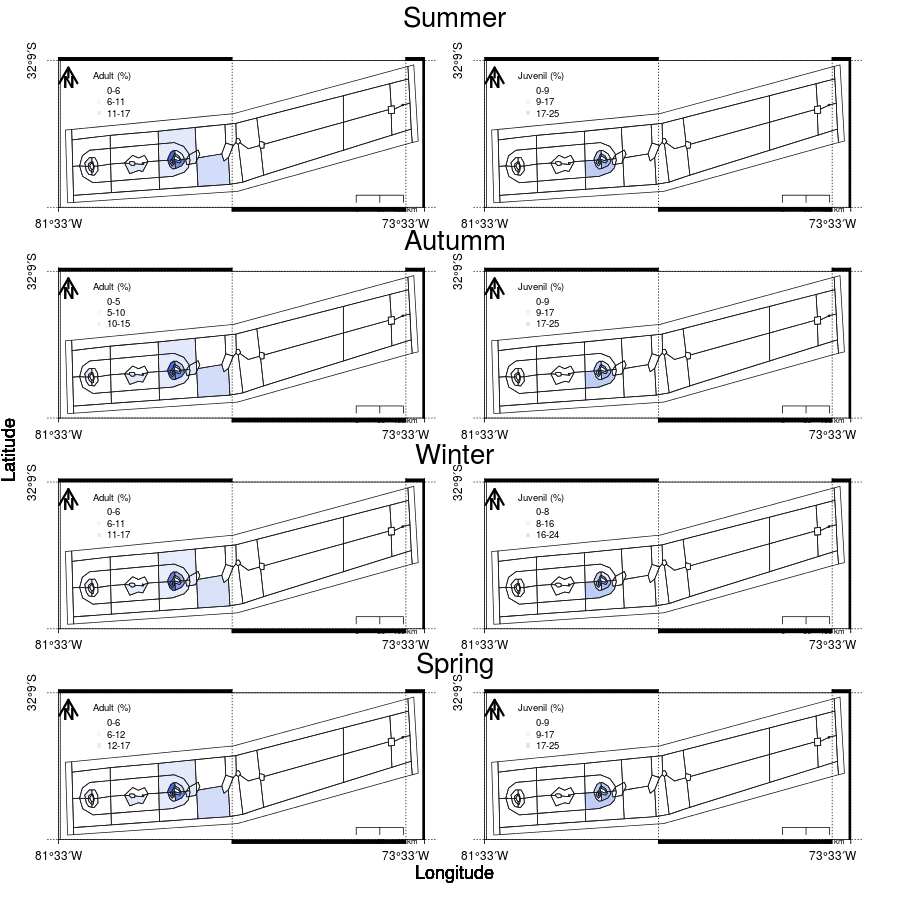
\includegraphics[width=.9\linewidth]{/home/demiurgo/Documents/PhD/Atlantis_Model/model_JFR/MandM/img/Breca_Distr.png}
        \caption{Horizontal distribution of Breca divided by ontogenetic stage (Juvenile and Adult) and by seasons}
        \end{figure}
\item Golden Crab spatial distribution

\begin{verbatim}
##-----------------------------------------#
##  obtener los limites de las capturas    #
##-----------------------------------------#
source('/home/demiurgo/Documents/PhD/Atlantis_Model/tools/General_tools/Atlantis_tools.R')
library(ascii)
options(asciiType = "org")
poly      <- read.poly('/home/demiurgo/Documents/PhD/Polygonos/Map/Polygons_20170510.csv')
centroids <- read.csv('/home/demiurgo/Documents/PhD/Functional_groups/location/Cover/centroids.csv')
## Reading data
lc  <- read.csv('/home/demiurgo/Documents/PhD/Functional_groups/location/juvenils/crustacean/spatial_size_crustaceans.csv')
lc2 <- FG(lc, 5)
lc2 <- lc2[complete.cases(lc2), ]
## By season
lc2$season.vat <- with(lc2,  ifelse(Month %in% c(1,2,3), 1,
                             ifelse(Month %in% c(4, 5, 6),2,
                             ifelse(Month %in% c(7,8,9), 3, 4))))
## Relocate the point inside the island to the closest polygons
lon    <- as.matrix(poly$coor[, c(seq(from = 1, to = dim(poly$coor)[2], by = 2))])
lat    <- as.matrix(poly$coor[, c(seq(from = 2, to = dim(poly$coor)[2], by = 2))])
points <- cbind(-lc2$Lon, -lc2$Lat)
for(island in c(49, 46)){
    is.poly <- na.omit(cbind(lon[order(poly$attrib$box_id), ][island,], lat[order(poly$attrib$box_id), ][island,]))
    points  <- move.point(points, centroids, is.poly)
}
lc2$Lon   <- -points[, 1]
lc2$Lat   <- -points[, 2]
lc.island <- split(lc2, lc2$FG)  # Split by functional Group
## Custacean
##---------------------------
## I use age of maturity reported based on the data base analysis
data.end <- NULL
for(cr in 1: length(lc.island)){
    crus           <- lc.island[[cr]]
    if(cr == 1){
        crus$Age   <- with(crus, ifelse(Cephalothorax_length > 106.62, 'Adult', 'Juvenil'))
    } else {
        crus$Age   <- with(crus, ifelse(Cephalothorax_length > 73.5,'Adult','Juvenil'))
    }
    crus$Mult  <- 1 ## each row has the value of one specie
    crus       <- split(crus, crus$Age)
    poly.dis   <- by.pol(poly, crus, la = 3, lo = 2, mult = 9, sea = 7, is.Crus = TRUE)
    nomb       <- colnames(poly.dis[[1]]$attrib)[7 : 8]
    poly.dis   <- clean(poly.dis, nomb)
    season     <- c('Summer', 'Autumm','Winter','Spring')
    png(paste0('img/',ifelse(cr == 1,'GCR','SPL'), '_Distr.png'), width = 900, height = 900)
    par(mfrow = c(4, 2), mar=c(3 ,2, 3, 2), oma = c(3, 3, 3, 2))
    titl <- c(0,-23.5,-46,-68)
    for(i in 1 : 4){
        for(fg in nomb){
            plot.map(poly.dis[[i]], leg.color = fg, specie = TRUE, leg = -81.33, save = FALSE, name = fg, PAR = FALSE)
        }
        mtext(season[i],  line = titl[i] , outer = TRUE,  cex = 2.3)
    }
    dev.off()
    ## table
    ## by functional group
    data.f  <- data.frame(Box = poly.dis[[1]]$attrib$box_id)
    ord     <- order(data.f)
    name.f  <- 'Box'
    for(fg in nomb){
        dbs  <- cbind(poly.dis[[1]]$attrib[, fg], poly.dis[[2]]$attrib[, fg],
                      poly.dis[[3]]$attrib[, fg], poly.dis[[4]]$attrib[, fg])
        if(all(dbs[, 1] %in% dbs[, 2], na.rm = TRUE)){
            ## all the seasons the same distribution
            data.f <- cbind(data.f, (dbs[, 1] / sum(dbs[, 1], na.rm = TRUE)))
            name.f <- c(name.f, paste0(ifelse(cr == 1,'GCR','SPL'),fg, 'all_seasons',sep = '_'))
        } else {
            for(s in 1 : 4){
                data.f <- cbind(data.f, (dbs[, s] / sum(dbs[, s], na.rm = TRUE)))
                name.f <- c(name.f,  paste(ifelse(cr == 1,'GCR','SPL'), fg, season[s], sep = '_'))
            }
        }
    }
    colnames(data.f) <- name.f
    data.f           <- t(data.f[ord, ])
    data.end         <- rbind(data.end, data.f)
}
cap              <- 'Proportion of FG by Box'
b                <- ascii(data.end, header = T,  include.rownames = TRUE, include.colnames = FALSE, caption=cap, digits=3)
print(b)
write.table(data.end, file = '/home/demiurgo/Documents/PhD/Functional_groups/location/juvenils/crustacean/Crus_dist_fin.csv', col.names = FALSE)
\end{verbatim}

\begin{center}
\begin{tabular}{lrrrrrrrrrrrrrrrrrrrrrrrrrrrrrrrrrrrrrrrrrrrrrrrrrrrrrrrrrrr}
 Box                 &  0.000  &  1.000  &  2.000  &  3.000  &  4.000  &  5.000  &  6.000  &  7.000  &  8.000  &  9.000  &  10.000  &  11.000  &  12.000  &  13.000  &  14.000  &  15.000  &  16.000  &  17.000  &  18.000  &  19.000  &  20.000  &  21.000  &  22.000  &  23.000  &  24.000  &  25.000  &  26.000  &  27.000  &  28.000  &  29.000  &  30.000  &  31.000  &  32.000  &  33.000  &  34.000  &  35.000  &  36.000  &  37.000  &  38.000  &  39.000  &  40.000  &  41.000  &  42.000  &  43.000  &  44.000  &  45.000  &  46.000  &  47.000  &  48.000  &  49.000  &  50.000  &  51.000  &  52.000  &  53.000  &  54.000  &  55.000  &  56.000  &  57.000  &  58.000  \\
\hline
 GCR_Adult_Summer    &         &         &         &         &         &         &  0.005  &         &         &         &          &          &          &          &          &          &          &          &          &          &          &          &          &          &          &   0.005  &   0.220  &          &          &          &          &          &   0.011  &   0.028  &   0.010  &   0.183  &   0.270  &   0.145  &   0.010  &          &          &          &          &          &          &          &          &          &          &          &          &   0.011  &   0.064  &   0.002  &   0.036  &          &          &          &          \\
 GCR_Adult_Autumm    &         &         &         &         &         &         &  0.006  &         &         &         &          &          &          &          &          &          &          &          &          &          &          &          &          &          &          &   0.005  &   0.221  &          &          &          &          &          &   0.005  &   0.028  &   0.010  &   0.184  &   0.272  &   0.146  &   0.010  &          &          &          &          &          &          &          &          &          &          &          &          &   0.011  &   0.064  &   0.002  &   0.036  &          &          &          &          \\
 GCR_Adult_Winter    &         &         &         &         &         &         &  0.006  &         &         &         &          &          &          &          &          &          &          &          &          &          &          &          &          &          &          &   0.005  &   0.222  &          &          &          &          &          &   0.003  &   0.029  &   0.011  &   0.184  &   0.273  &   0.146  &   0.010  &          &          &          &          &          &          &          &          &          &          &          &          &   0.011  &   0.065  &   0.002  &   0.036  &          &          &          &          \\
 GCR_Adult_Spring    &         &         &         &         &         &         &  0.006  &         &         &         &          &          &          &          &          &          &          &          &          &          &          &          &          &          &          &   0.005  &   0.221  &          &          &          &          &          &   0.007  &   0.028  &   0.010  &   0.183  &   0.271  &   0.145  &   0.010  &          &          &          &          &          &          &          &          &          &          &          &          &   0.011  &   0.064  &   0.002  &   0.036  &          &          &          &          \\
 GCR_Juvenil_Summer  &         &         &         &         &         &         &  0.005  &         &         &         &          &          &          &          &          &          &          &          &          &          &          &          &          &          &          &   0.002  &   0.015  &          &          &          &          &          &   0.005  &   0.002  &          &   0.613  &   0.055  &   0.054  &          &          &          &          &          &          &          &          &          &          &          &          &          &   0.046  &   0.160  &          &   0.045  &          &          &          &          \\
 GCR_Juvenil_Autumm  &         &         &         &         &         &         &  0.004  &         &         &         &          &          &          &          &          &          &          &          &          &          &          &          &          &          &          &   0.001  &   0.031  &          &          &          &          &          &   0.004  &   0.001  &          &   0.549  &   0.049  &   0.048  &          &          &          &          &          &          &          &          &          &          &          &          &          &   0.041  &   0.229  &          &   0.040  &          &          &          &          \\
 GCR_Juvenil_Winter  &         &         &         &         &         &         &  0.005  &         &         &         &          &          &          &          &          &          &          &          &          &          &          &          &          &          &          &   0.002  &   0.056  &          &          &          &          &          &   0.005  &   0.002  &          &   0.629  &   0.056  &   0.056  &          &          &          &          &          &          &          &          &          &          &          &          &          &   0.047  &   0.097  &          &   0.046  &          &          &          &          \\
 GCR_Juvenil_Spring  &         &         &         &         &         &         &  0.005  &         &         &         &          &          &          &          &          &          &          &          &          &          &          &          &          &          &          &   0.002  &   0.018  &          &          &          &          &          &   0.005  &   0.002  &          &   0.677  &   0.060  &   0.060  &          &          &          &          &          &          &          &          &          &          &          &          &          &   0.051  &   0.069  &          &   0.049  &          &          &          &          \\
 SPL_Adult_Summer    &         &         &         &         &         &         &  0.000  &         &         &         &          &          &          &          &          &          &          &          &          &   0.000  &          &          &   0.001  &   0.006  &          &   0.001  &   0.001  &          &          &          &          &          &   0.000  &          &   0.000  &   0.001  &   0.001  &   0.004  &   0.002  &          &          &   0.002  &   0.001  &   0.004  &   0.002  &          &          &          &          &          &          &   0.128  &   0.060  &   0.120  &   0.132  &   0.201  &   0.066  &   0.133  &   0.134  \\
 SPL_Adult_Autumm    &         &         &         &         &         &         &  0.000  &         &         &         &          &          &          &          &          &          &          &          &          &   0.000  &          &          &   0.001  &   0.000  &          &   0.001  &   0.001  &          &          &          &          &          &   0.000  &          &   0.000  &   0.002  &   0.001  &   0.004  &   0.002  &          &          &   0.002  &   0.001  &   0.004  &   0.002  &          &          &          &          &          &          &   0.129  &   0.060  &   0.121  &   0.133  &   0.202  &   0.066  &   0.134  &   0.134  \\
 SPL_Adult_Winter    &         &         &         &         &         &         &  0.000  &         &         &         &          &          &          &          &          &          &          &          &          &   0.000  &          &          &   0.001  &   0.006  &          &   0.001  &   0.001  &          &          &          &          &          &   0.000  &          &   0.000  &   0.002  &   0.001  &   0.004  &   0.002  &          &          &   0.002  &   0.001  &   0.004  &   0.002  &          &          &          &          &          &          &   0.128  &   0.060  &   0.120  &   0.132  &   0.201  &   0.066  &   0.133  &   0.133  \\
 SPL_Adult_Spring    &         &         &         &         &         &         &  0.000  &         &         &         &          &          &          &          &          &          &          &          &          &   0.000  &          &          &   0.001  &   0.013  &          &   0.001  &   0.001  &          &          &          &          &          &   0.000  &          &   0.000  &   0.002  &   0.001  &   0.004  &   0.002  &          &          &   0.002  &   0.001  &   0.004  &   0.002  &          &          &          &          &          &          &   0.127  &   0.059  &   0.119  &   0.131  &   0.200  &   0.065  &   0.132  &   0.133  \\
 SPL_Juvenil_Summer  &         &         &         &         &         &         &         &         &         &         &          &          &          &          &          &          &          &          &          &          &          &          &   0.010  &   0.010  &          &          &          &          &          &          &          &          &          &          &          &          &          &   0.010  &   0.010  &          &          &   0.010  &          &          &          &          &          &          &          &          &          &   0.297  &   0.104  &   0.228  &   0.038  &   0.069  &   0.025  &   0.080  &   0.109  \\
 SPL_Juvenil_Autumm  &         &         &         &         &         &         &         &         &         &         &          &          &          &          &          &          &          &          &          &          &          &          &   0.010  &   0.010  &          &          &          &          &          &          &          &          &          &          &          &          &          &   0.010  &   0.010  &          &          &   0.010  &          &          &          &          &          &          &          &          &          &   0.294  &   0.107  &   0.157  &   0.039  &   0.071  &   0.025  &   0.082  &   0.173  \\
 SPL_Juvenil_Winter  &         &         &         &         &         &         &         &         &         &         &          &          &          &          &          &          &          &          &          &          &          &          &   0.010  &   0.010  &          &          &          &          &          &          &          &          &          &          &          &          &          &   0.010  &   0.010  &          &          &   0.010  &          &          &          &          &          &          &          &          &          &   0.292  &   0.109  &   0.083  &   0.040  &   0.073  &   0.026  &   0.085  &   0.240  \\
 SPL_Juvenil_Spring  &         &         &         &         &         &         &         &         &         &         &          &          &          &          &          &          &          &          &          &          &          &          &   0.010  &   0.010  &          &          &          &          &          &          &          &          &          &          &          &          &          &   0.010  &   0.010  &          &          &   0.010  &          &          &          &          &          &          &          &          &          &   0.292  &   0.109  &   0.083  &   0.040  &   0.073  &   0.026  &   0.085  &   0.240  \\
\end{tabular}
\end{center}


\begin{itemize}
\item Some considerations
\begin{itemize}
\item For lobster in winter distribution I use the mean between spring and autumm
\item For Large pelagic fish, Mollusca, Octupus, Small bentic fish and small crustacean, I used the average distribution for all the seasons.
\end{itemize}
\end{itemize}
\end{itemize}
\end{itemize}

\item Vertical distribution
\label{sec-5-2-1-6-2}%
\begin{itemize}
\item \textbf{Deph Distribution}

\begin{center}
\begin{tabular}{lrrl}
 Functional Groups  &  Min  &   Max  &  Author                                                               \\
\hline
 SPL                &    2  &   250  &  Retamal \& Arana 2000  - Descripcion y distribucion de 5 decapodos   \\
 GCR                &  100  &  1000  &  Arana et al 2000  -  Pesca exploratoria                              \\
 BRC                &   20  &   300  &  Arana \& Vega 2000  -  Pesca exploratoria espinel and billy DB       \\
 ORO                &  500  &  1000  &  Niklitschek 2007 evaluacion hidroacustica alfonsino y otange roughy  \\
 ALF                &  200  &   600  &  Niklitschek 2007 evaluacion hidroacustica alfonsino y otange roughy  \\
 LPF                &    0  &   200  &  Billy data base                                                      \\
 SPF                &    0  &   250  &  Billy data base                                                      \\
 SBF                &    0  &   250  &  Billy data base                                                      \\
 LBF                &    0  &   250  &  Billy data base                                                      \\
 VID                &    3  &   150  &  IUCN and fish-base                                                   \\
 ANG                &    0  &   300  &  Arana 2000 - PEsca exploratoria con trampa                           \\
 CHO                &   20  &   600  &  Fishbase                                                             \\
 COR                &   50  &  1000  &  Data base \&   Niklitschek 2010                                      \\
 MPF                &    0  &  5000  &  Fish base                                                            \\
\end{tabular}
\end{center}


\begin{itemize}
\item \textbf{NOTE} For SBF and LBF it was necesary increase the maximum depth using the distriburion observed by Yañes et al. (2008; Seamount biodiversity report)
\end{itemize}
\item \textbf{Day-nigth distribution}
\begin{itemize}
\item Vertebrates

\begin{verbatim}
#-----------------------------------------#
#  obtener los limites de las capturas    #
#-----------------------------------------#
rm(list = ls())
## Data~~~~~~~~~~~~~~~~~~~~~~~~~~~~~~~~~~~~~~~~
library(ascii)
options(asciiType = "org")
source('/home/demiurgo/Documents/PhD/Atlantis_Model/tools/General_tools/Atlantis_tools.R')
lc <- read.csv('/home/demiurgo/Documents/PhD/Functional_groups/Depth/Species_depth.csv')
layer.depths      <- c(20, 50, 150, 250, 400, 650, 1000, 4300)
avgph             <- mean(lc$Captain_fathom,  na.rm = TRUE)
lc$Captain_fathom <- ifelse(is.na(lc$Captain_fathom), avgph, lc$Captain_fathom)
lc$Depth          <- ifelse(is.na(lc$Depth), lc$Captain_fathom * lc$Braz, lc$Depth)
lc$Total_unit[is.na(lc$Total_unit)]      <- 0    # Removing the NA
lc$Total_unit[which(lc$Total_unit == 0)] <- 1    # Removing the 0
#~~~~~~~~~~~~~~~~~~~~~~~~~~~~~~~~~~~~~~~~~~~~~~~~~~~~~~~~~~~~~~~~~~~~~~~~~~~~~~~~
##Divdiden by layer
lc$layer <- ifelse(lc$Depth <= layer.depths[1], 1,
            ifelse(lc$Depth <= layer.depths[2], 2,
            ifelse(lc$Depth <= layer.depths[3], 3,
            ifelse(lc$Depth <= layer.depths[4], 4,
            ifelse(lc$Depth <= layer.depths[5], 5,
            ifelse(lc$Depth <= layer.depths[6], 6,
            ifelse(lc$Depth <= layer.depths[7], 7, 8)))))))
## Expand rows based on the values on the column
lc <- dup.row(lc, 2)
## Grupos funcionales
lc <- FG(lc, 1)

#lc.fg$SPF[which(lc.fg$SPF$layer==3),]
##-----------
##  Divide by functional group
##---------------
lc.fg      <- split(lc, lc$FG)           # split by functional group
lc.fg      <- lc.fg[ - c(3, 8)]          # Remove the BCA and octopus
lc.fg[[3]] <- stage(lc.fg[[3]], 6, 282)  # Based on Ribara thesis
##  Distribution by layers
depth <- data.frame(specie = names(lc.fg),
                    min    = rep(0, length(lc.fg)),
                    max    = rep(8, length(lc.fg)))
##++++++++++++++++++++
## Real depth location
##++++++++++++++++++++
out <- hist.deph(lc.fg, col.val = 8, dep.lim = depth, n.file = 'img/Functional_groups')
out <- t(out)
colnames(out) <- paste('layer', rep(8 : 1))
cap           <- 'Proportion of FG by layer'
b             <- ascii(out, header = T,  include.rownames = TRUE, include.colnames = TRUE, caption=cap, digits=3)
print(b)
\end{verbatim}
\begin{table}[htb]
\caption{Proportion of FG by layer}
\begin{center}
\begin{tabular}{lrrrrrrrr}
              &  layer 8  &  layer 7  &  layer 6  &  layer 5  &  layer 4  &  layer 3  &  layer 2  &  layer 1  \\
\hline
 ALF          &    0.000  &    0.051  &    0.268  &    0.580  &    0.046  &    0.055  &    0.000  &    0.000  \\
 ANG          &    0.000  &    0.000  &    0.000  &    0.000  &    0.000  &    0.146  &    0.491  &    0.363  \\
 BRC-Adult    &    0.000  &    0.000  &    0.000  &    0.085  &    0.120  &    0.668  &    0.071  &    0.056  \\
 BRC-Juvenil  &    0.000  &    0.000  &    0.000  &    0.013  &    0.095  &    0.729  &    0.106  &    0.058  \\
 CHO          &    0.000  &    0.144  &    0.317  &    0.183  &    0.224  &    0.131  &    0.001  &    0.001  \\
 LBF          &    0.000  &    0.122  &    0.269  &    0.491  &    0.040  &    0.054  &    0.020  &    0.003  \\
 LPF          &    0.000  &    0.000  &    0.000  &    0.000  &    0.003  &    0.030  &    0.125  &    0.842  \\
 ORO          &    0.000  &    0.649  &    0.347  &    0.004  &    0.000  &    0.000  &    0.000  &    0.000  \\
 SBF          &    0.000  &    0.122  &    0.268  &    0.489  &    0.041  &    0.075  &    0.002  &    0.002  \\
 SCR          &    0.000  &    0.000  &    0.000  &    0.000  &    0.000  &    0.000  &    1.000  &    0.000  \\
 SPF          &    0.000  &    0.000  &    0.000  &    0.000  &    0.069  &    0.435  &    0.165  &    0.330  \\
 VID          &    0.000  &    0.000  &    0.000  &    0.000  &    0.005  &    0.269  &    0.585  &    0.140  \\
\end{tabular}
\end{center}
\end{table}

    \begin{figure}[htb]
    \centering
    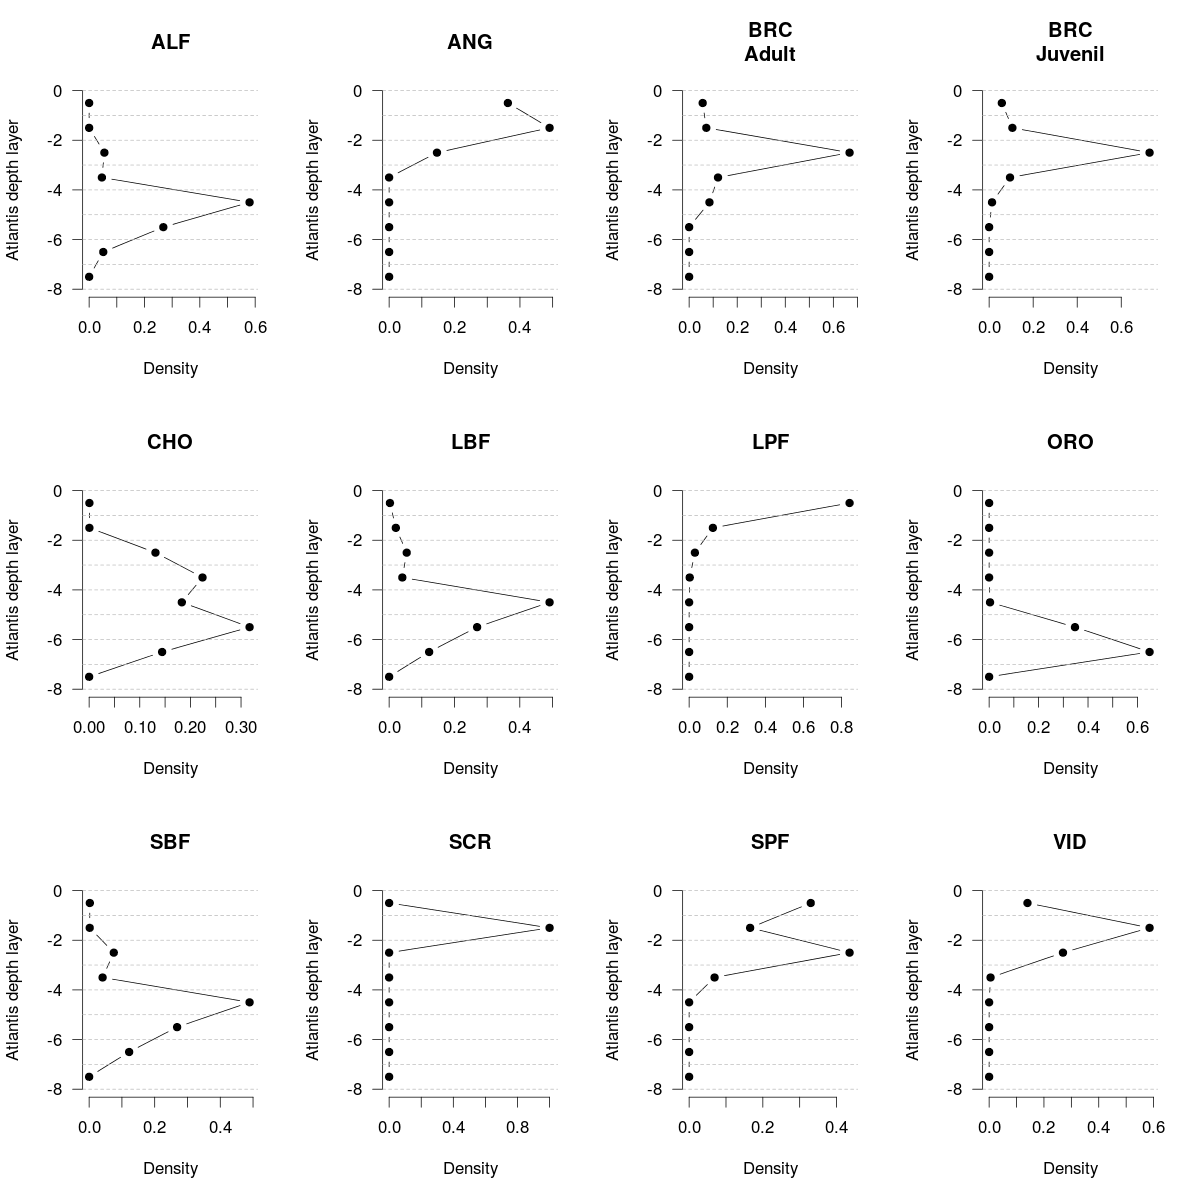
\includegraphics[width=.9\linewidth]{/home/demiurgo/Documents/PhD/Atlantis_Model/model_JFR/MandM/img/Functional_groups.png}
    \caption{Vertical distribution of the vertebrate FG}
    \end{figure}
\item Invertebrates

\begin{verbatim}
rm(list = ls())
library(ascii)
options(asciiType = "org")
source('/home/demiurgo/Documents/PhD/Atlantis_Model/tools/General_tools/Atlantis_tools.R')
zoo <- read.csv('/home/demiurgo/Documents/PhD/Functional_groups/Depth/COP-EUF/Zooplancton.csv')
##Divdiden by layer
layer.depths <- c(20, 50, 150, 250, 400, 650, 1000, 4300)
zoo$layer    <- ifelse(zoo$Depth <= layer.depths[1], 1,
                ifelse(zoo$Depth <= layer.depths[2], 2,
                ifelse(zoo$Depth <= layer.depths[3], 3,
                ifelse(zoo$Depth <= layer.depths[4], 4,
                ifelse(zoo$Depth <= layer.depths[5], 5,
                ifelse(zoo$Depth <= layer.depths[6], 6,
                ifelse(zoo$Depth <= layer.depths[7], 7, 8)))))))
## Expand rows based on the values on the column
zoo$FG <- paste(zoo$FG, zoo$time, sep = '_')
zoo.dup     <- dup.row(zoo, 3)
## Grupos funcionales
zoo.ly      <- split(zoo.dup, zoo.dup$FG)
depth <- data.frame(specie = names(zoo.ly),
                    min    = rep(0, length(zoo.ly)),
                    max    = rep(8, length(zoo.ly)))
##++++++++++++++++++++
## Real depth location
##++++++++++++++++++++
out <- hist.deph(zoo.ly, col.val = 5, dep.lim = depth, n.file = 'img/Zooplankton')
out <- t(out)
colnames(out) <- paste('layer', rep(8 : 1))
cap           <- 'Proportion of zooplankton by layer'
b             <- ascii(out, header = T,  include.rownames = TRUE, include.colnames = TRUE, caption=cap, digits=3)
print(b)
\end{verbatim}

\begin{center}
\begin{tabular}{lrrrrrrrr}
            &  layer 8  &  layer 7  &  layer 6  &  layer 5  &  layer 4  &  layer 3  &  layer 2  &  layer 1  \\
\hline
 LZO_Day    &    0.000  &    0.000  &    0.000  &    0.050  &    0.269  &    0.516  &    0.053  &    0.112  \\
 LZO_Nigth  &    0.000  &    0.000  &    0.000  &    0.000  &    0.000  &    0.362  &    0.024  &    0.615  \\
 MZO_Day    &    0.000  &    0.000  &    0.000  &    0.007  &    0.077  &    0.669  &    0.244  &    0.003  \\
 MZO_Night  &    0.000  &    0.000  &    0.000  &    0.179  &    0.174  &    0.025  &    0.531  &    0.092  \\
\end{tabular}
\end{center}


\begin{itemize}
\item Lobster and Golden Crab Vertical distribution

\begin{verbatim}
rm(list = ls())
library(ascii)
options(asciiType = "org")
source('/home/demiurgo/Documents/PhD/Atlantis_Model/tools/General_tools/Atlantis_tools.R')
crus <- read.csv('/home/demiurgo/Documents/PhD/Functional_groups/Depth/depth_crustaceans.csv')
##Divdiden by layer
layer.depths <- c(20, 50, 150, 250, 400, 650, 1000, 4300)
crus$layer    <- ifelse(crus$depth <= layer.depths[1], 1,
                ifelse(crus$depth <= layer.depths[2], 2,
                ifelse(crus$depth <= layer.depths[3], 3,
                ifelse(crus$depth <= layer.depths[4], 4,
                ifelse(crus$depth <= layer.depths[5], 5,
                ifelse(crus$depth <= layer.depths[6], 6,
                ifelse(crus$depth <= layer.depths[7], 7, 8)))))))
## By functional group
crus_FG <- FG(crus, 2)
## Expand rows based on the values on the column
crus_FG <- crus_FG[-which(crus_FG$total == 0), ]
crus.dup     <- dup.row(crus_FG, 4)
## Functinal groups
crus.ly      <- split(crus.dup, crus.dup$FG)
depth <- data.frame(specie = names(crus.ly),
                    min    = rep(0, length(crus.ly)),
                    max    = rep(8, length(crus.ly)))
##++++++++++++++++++++
## Real depth location
##++++++++++++++++++++
out <- hist.deph(crus.ly, col.val = 7, dep.lim = depth, n.file = 'img/crustacean.prn')
out <- t(out)
colnames(out) <- paste('layer', rep(8 : 1))
cap           <- 'Vertical distribution of crustacean by layer'
b             <- ascii(out, header = T,  include.rownames = TRUE, include.colnames = TRUE, caption=cap, digits=3)
print(b)
\end{verbatim}

\begin{center}
\begin{tabular}{lrrrrrrrr}
      &  layer 8  &  layer 7  &  layer 6  &  layer 5  &  layer 4  &  layer 3  &  layer 2  &  layer 1  \\
\hline
 GCR  &        0  &    0.000  &    0.615  &    0.318  &    0.067  &        0  &        0  &        0  \\
 SPL  &    0.000  &    0.000  &   0.1799  &   0.1795  &   0.5421  &    0.278  &        0  &        0  \\
\end{tabular}
\end{center}



\begin{table}[htb]
\caption{Proportion by layer of other invertebrates}
\begin{center}
\begin{tabular}{llrrrrrrrrl}
 FG   &  Light  &  Deepest layer  &     &     &         &         &        &        &  Surface  &  Source          \\
\hline
 OCT  &         &              0  &  0  &  0  &  0.017  &  0.183  &  0.33  &  0.31  &     0.16  &                  \\
 SUR  &  D      &              1  &  0  &  0  &      0  &      0  &     0  &     0  &        0  &  Billy Database  \\
 SUR  &  N      &              1  &  0  &  0  &      0  &      0  &     0  &     0  &        0  &  Billy Database  \\
 MOL  &  D      &              1  &  0  &  0  &      0  &      0  &     0  &     0  &        0  &  Billy Database  \\
 MOL  &  N      &              1  &  0  &  0  &      0  &      0  &     0  &     0  &        0  &  Billy Database  \\
\end{tabular}
\end{center}
\end{table}

\end{itemize}
\begin{figure}[htb]
    \centering
    \includegraphics[width=.9\linewidth]{/home/demiurgo/Documents/PhD/Functional_groups/Depth/COP-EUF/copeuf.png}
    \caption{Relative vertical Distribution of Medium (Copepods) and Large (Eufausiid) zooplancton according to their maximimum and minimum depth}
    \end{figure}
\item MPF

\begin{center}
\begin{tabular}{lrrrrrrrr}
 Layer  &     1  &     2  &     3  &    4  &     5  &     6  &     7  &     8  \\
\hline
 Nigth  &  0.15  &  0.24  &  0.26  &  0.2  &  0.12  &  0.03  &     0  &     0  \\
 Day    &     0  &     0  &     0  &    0  &  0.15  &  0.35  &  0.39  &  0.11  \\
\end{tabular}
\end{center}


\end{itemize}
\begin{figure}[htb]
  \centering
  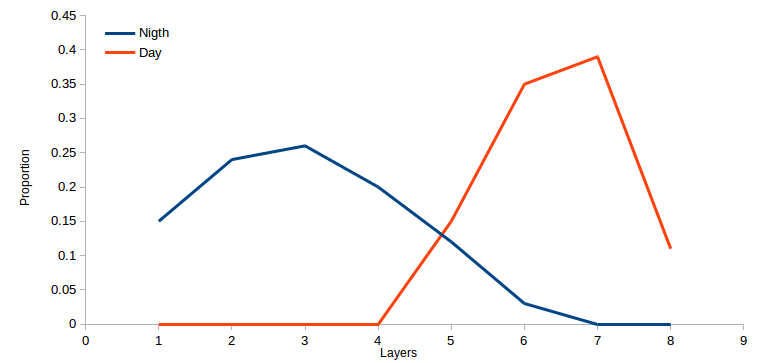
\includegraphics[width=.9\linewidth]{/home/demiurgo/Documents/PhD/Atlantis_Model/model_JFR/MandM/img/mpf_vert.png}
  \caption{Relative vertical Distribution of Mesopelagic fish}
  \end{figure}
\end{itemize}

\item Speed movement\\
\label{sec-5-2-1-6-3}%
\begin{center}
\begin{tabular}{lrlll}
 Functional group  &  Speed m.hr-1  &  Specie or group  &  Real speed reported  &  Source                                   \\
\hline
 SPL               &          1260  &  Lobster          &  35 cm*sec-1          &  Childress and Jury. Chapter 3-behaviour  \\
 GCR               &           450  &  Gost crab        &  0.45 K*h             &  Tully and andrus 2011                    \\
 BRC               &          2228  &  Acanthuridae     &  61.9cm*s             &  Fulton et al. 2005                       \\
 ORO               &          1440  &  Trachinidae      &  0.4 m*s              &  Fishbase                                 \\
\end{tabular}
\end{center}



\begin{itemize}
\item Look for the depth distribution of the functional groups
  For this, I use the information in SETas model and references
\end{itemize}

\item Migration
\label{sec-5-2-1-6-4}%
\begin{itemize}
\item \textbf{Day of migration}

\begin{center}
\begin{tabular}{lll}
 Species   &  Month                &  Reference        \\
\hline
 Vidriola  &  Spring-Summer        &  Arana 2000b      \\
 Whales    &  Leave during winter  &  Whales in Chile  \\
 Birds     &  Srping and summer    &  OIKONOS          \\
\end{tabular}
\end{center}


\begin{itemize}
\item \textbf{Vidriola}
\begin{itemize}
\item catch analisys to Estimate the months when the vidriola is leaving the JFRE

\begin{verbatim}
##libraries
library(ggplot2)
rblue   <- rgb(t(col2rgb("royalblue")), alpha = 100, maxColorValue = 255)
#setwd("/home/demiurgo/Documents/PhD/Functional_groups/Migration/Vidriola/")
vid.io            <- read.table('/home/demiurgo/Documents/PhD/Functional_groups/Migration/Vidriola/Vid_month.txt', sep = ' ', header = TRUE)
s                 <- qplot(as.factor(Month), Weight, data = vid.io, geom=c("boxplot"), xlab = 'Month', ylab = 'Biomass (kg)')
mean.month        <- with(vid.io, aggregate(Weight~as.factor(Month), FUN = mean))
mean.month$Weight <- mean.month$Weight / sum(mean.month$Weight)
png('img/migration_Vid.png', width = 1000, height = 1000)
par(mar=c(5,4,4,5)+.1, cex = 1.4)
boxplot(Weight ~ as.factor(Month), data = vid.io, col = 'royalblue', bty = 'n', outline = FALSE, xlab = 'Months', ylab = 'Catch (Number)', border = rblue,las = 1,
        main = 'Vidriola Migration')
par(new = TRUE)
plot(as.numeric(mean.month[, 1]), mean.month[, 2], type = 'b', pch = 20, col = 2, axes = F, xlab = '', ylab = '', bty = 'n')
axis(4, col = 2, las = 1)
mtext("Proportion", side=4, line=3)
dev.off()
\end{verbatim}
\end{itemize}
\end{itemize}
\end{itemize}
       \begin{figure}[htb]
       \centering
       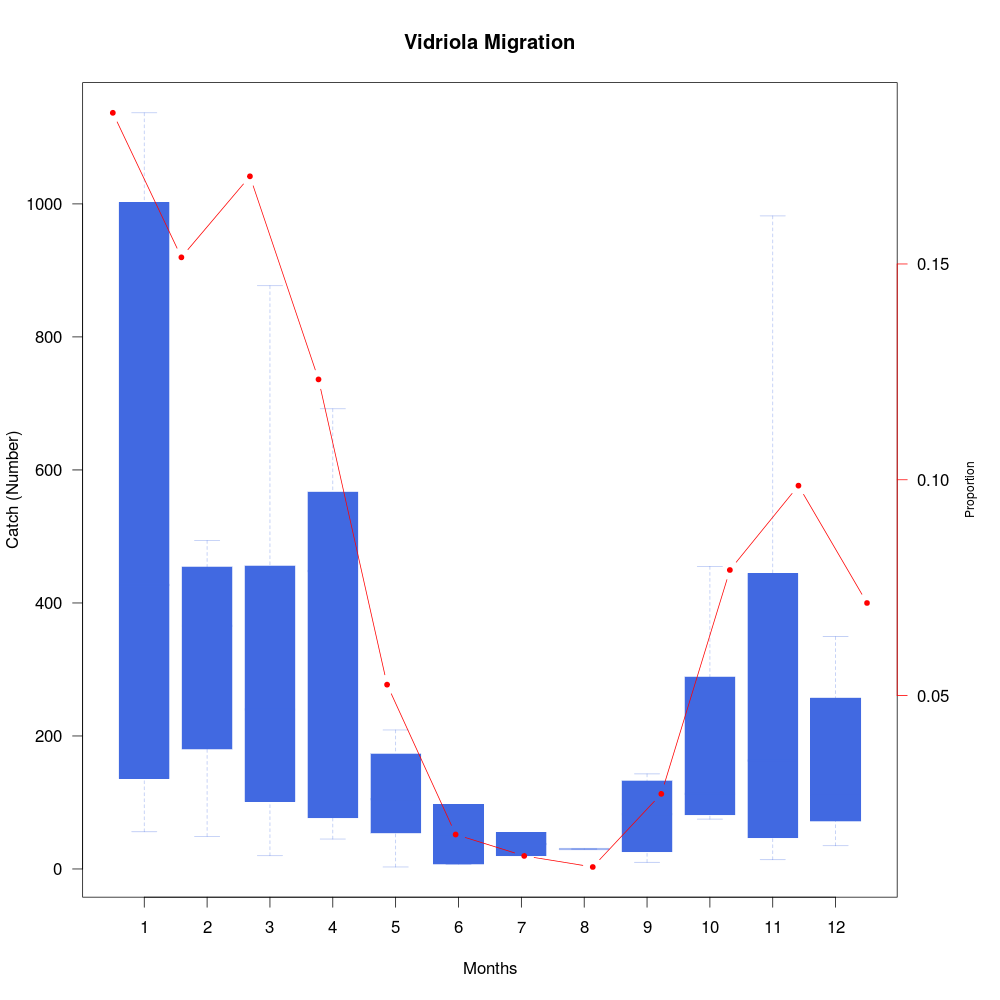
\includegraphics[width=.9\linewidth]{/home/demiurgo/Documents/PhD/Atlantis_Model/model_JFR/MandM/img/migration_Vid.png}
       \caption{Catch and abundance of vidriola during the months}
       \end{figure}


\begin{itemize}
\item \textbf{Initial condition (Abundance) for migrating species}
\begin{itemize}
\item \underline{Vidriola}
         I use the length converted catch curve to estimate Z.

\begin{verbatim}
library(ascii)
options(asciiType="org")
##-------------------------------------#
## Estimation of abundance using APV   #
##------------------------------------ #
vid.io            <- read.table('/home/demiurgo/Documents/PhD/Functional_groups/Migration/Vidriola/Vid_month.txt', sep = ' ', header = TRUE)
lfd               <- read.csv('/home/demiurgo/Documents/PhD/Functional_groups/Migration/Vidriola/VID.csv')
sum.season        <- with(vid.io, aggregate(Weight~as.factor(Season), FUN = sum))
dist              <- lfd$count/sum(lfd$count)
mean.month        <- with(vid.io, aggregate(Weight~as.factor(Month), FUN = mean))
mean.month$Weight <- mean.month$Weight / sum(mean.month$Weight)
vec               <- c(t(outer(sum.season[8:10,2],mean.month[,2])))
total             <- t(outer(vec, dist))
dates             <- format(seq(as.Date('2013-01-30'), by='months',length.out=36), '%d/%m/%Y')
colnames(total)   <- as.character(dates)
total             <- cbind(id=lfd[,2],total)
## write.table(total, 'Vid_lccc.txt',row.names=FALSE,sep=',')
##~~~~~~~~~~~~~~~~~~~~~~~~~~~~~~~~~~~~~~~~~~~~~~~~~~~~#
##  Using length converted catch curve to estimate z  #
##~~~~~~~~~~~~~~~~~~~~~~~~~~~~~~~~~~~~~~~~~~~~~~~~~~~~#
## source('ElefanI.R')
source('/home/demiurgo/Documents/PhD/Functional_groups/Migration/Vidriola/Lccc.R')
## ElefanI(data, vbplot = TRUE)
data <- '/home/demiurgo/Documents/PhD/Functional_groups/Migration/Vidriola/Vid_lccc.txt'
dat  <- Lccc(data, Linf = 964.95, K = 0.82, auto = TRUE, save = TRUE, quiet = TRUE)
Z    <- dat$Z_Estimate[1]
Z    <- 1.81 ## VAlue estimated using LCCC
M    <- 0.2
## -  -  -  -  -  -  -  -  -  -  -  -  -  - #
## Last abundance  Using Baranov equation    #
## -  -  -  -  -  -   -  -  -  -  -  -  - - #
abun.l <- data.frame(Season = c(2011 : 2015), Abundance = sum.season[6:10, 2] * Z) / ((Z - M) * (1 - exp( -  Z)))
cap    <- "Reconstruction of the abundance by using the Baranov equation"
b      <- ascii(abun.l, header = T, include.rownames = FALSE, include.colnames = T, caption=cap)
print(b)
\end{verbatim}
\end{itemize}
\end{itemize}
\begin{table}[htb]
\caption{Reconstruction of the abundance by using the Baranov equation}
\begin{center}
\begin{tabular}{rr}
  Season  &  Abundance  \\
\hline
 1493.48  &    1477.29  \\
 1494.23  &    2234.08  \\
 1494.97  &    7038.28  \\
 1495.71  &    6276.84  \\
 1496.45  &    8334.10  \\
\end{tabular}
\end{center}
\end{table}


          \begin{figure}[htb]
          \centering
          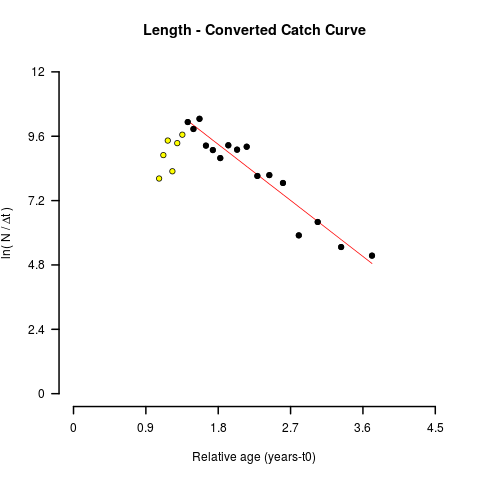
\includegraphics[width=.9\linewidth]{/home/demiurgo/Documents/PhD/Atlantis_Model/model_JFR/MandM/img/lccc.png}
          \caption{Estimation of Z using the length converted catch curve aproximation}
          \end{figure}

\begin{itemize}
\item \underline{Whales}
\begin{itemize}
\item Relative Abundance
\end{itemize}

\begin{center}
\begin{tabular}{lrl}
 Year          &  Abundance index  &  Reference                                \\
\hline
 1997-1998     &             0.15  &  Huke and Gaete 1998 (sensu Aguayo 1998)  \\
 1958          &            14.35  &  Clarrke (1962)                           \\
 1964          &             1.25  &  Clarke (1998)                            \\
 1994 - May    &             1.14  &  Aguayo-lobo 1998                         \\
 1995-sep      &            50.63  &  Aguayo-lobo 1998                         \\
 1995-Jun,jul  &             1.89  &  Aguayo-lobo 1998                         \\
 1997          &             2.71  &  Aguayo lobo 1998                         \\
 1982          &                1  &  Gallardo y Pastene                       \\
 1994-May      &             0.13  &  Aguallo-lobo 1998                        \\
 1994-sept     &             0.25  &  Aguallo-Lobo 1998                        \\
 1995-sept     &             0.63  &  Aguallo-Lobo 1998                        \\
\end{tabular}
\end{center}


          - Abundance (N) - Information from the IWC (2016)

\begin{center}
\begin{tabular}{lrrrrr}
 hemisphere  &  Sperm-whale  &  Humpback Whale  &  Blue Whale  &  Right Whale  &  Total  \\
\hline
 South       &         1905  &              76  &          60  &           87  &   2128  \\
\end{tabular}
\end{center}



           - Value using the maximun available number
            19105
\item \underline{Dolphins}
         I use the double of whales
\item \underline{Birds}
         The main seabird in the JFRE is the fardela
          \textbf{Oikonos tag information}   :  8601 individuals
\item Estimation of Reserve weight and structural weight
\begin{itemize}
\item The convertion from normal weight need to be done in following steps (remember that the ratios can change,  this is a rule of thum)
\item Frist  : The weight need to be in mg (miligrams)
\item Second : pass from wet to dry weight
\begin{itemize}
\item \( Weight(mg)_{dry}  = Weigth(mg)_{wet} / 20 \)
\end{itemize}
\item Third  : From dry weight to Nitrogen
\begin{itemize}
\item \(N(mg) = Weight(mg)_{dry} / 5.7\)
\end{itemize}
\item Forth  : Conversion to Structural weight and Reserve weight
\end{itemize}
\end{itemize}
      The ratio between structural weigth and reserve weight is 1:2.65
\begin{itemize}
\item \underline{Vidriola}

\begin{verbatim}
library(ascii)
options(asciiType="org")
##-----------------------------------------------#
##     Estimation of Wl for Vidriola             #
##-----------------------------------------------#

wl <- read.csv('/home/demiurgo/Documents/PhD/Functional_groups/Migration/Vidriola/Vid_WL.prn')
## ~~~~~~~~~~~~~~~~~~~~~~~~~~~~~~~~~~~~~~~~~~~~~~~~~~~~~~~~~~~~~~~~~~~~~~~~~~~~~~~~ ##
## ~                     Estimation of length weight relationship                 ~ ##
## ~~~~~~~~~~~~~~~~~~~~~~~~~~~~~~~~~~~~~~~~~~~~~~~~~~~~~~~~~~~~~~~~~~~~~~~~~~~~~~~~ ##
WL.relationship <- function(alfa, beta, len){
    weight <- alfa * len ^ beta
    return(weight)
}
len.obs <- wl$Fork_len
wei.obs <- wl$Weight
res     <- nls(wei.obs ~ WL.relationship(alfa, beta, len.obs), start = c(alfa = 0.02, beta = 1.7))
param   <- coefficients(res)
av.size <- c(580.2, 667.4, 776.4)
t.wei   <- WL.relationship(param[1],param[2], av.size)
png('img/wl.vid.png', height=1000, width=1000)
par(cex = 1.4)
plot(len.obs, wei.obs,pch = 19, col = 'grey', bty = 'n', xlab = 'fork length (mm)', ylab = 'weight (g)')
lines(len.obs,WL.relationship(param[1], param[2],len.obs),col = 2)
points(av.size, t.wei, pch = 19)
 invisible(dev.off())

## Wet to dry conversion
t.wei <- (t.wei / 20) * 1000 ## conversion from g to mg

## From dry weight to nitrogen
t.wei <- t.wei / 5.7

##--------------------------------------------------------------------------
## Generaly the ratio between structural weight and reserve weight is 1:2.65
##  -  -  -  -  -  -  -  -  -  -  -  -  -  -  -  -  -  -  -  -  -  -  -  -  -  -
factor  <- t.wei / 3.65
out     <- data.frame(structural = factor, reserve = factor * 2.65)

cap <- "Structural and reserve weight for Vidriola"
b   <- ascii(out, header = T, include.rownames = FALSE, include.colnames = T, caption=cap)
print(b)
\end{verbatim}
\end{itemize}
\begin{table}[htb]
\caption{Structural and reserve weight for Vidriola}
\begin{center}
\begin{tabular}{rr}
 structural  &   reserve  \\
\hline
    5640.62  &  14947.64  \\
    8513.40  &  22560.50  \\
   13281.82  &  35196.83  \\
\end{tabular}
\end{center}
\end{table}

       \begin{figure}[htb]
       \centering
       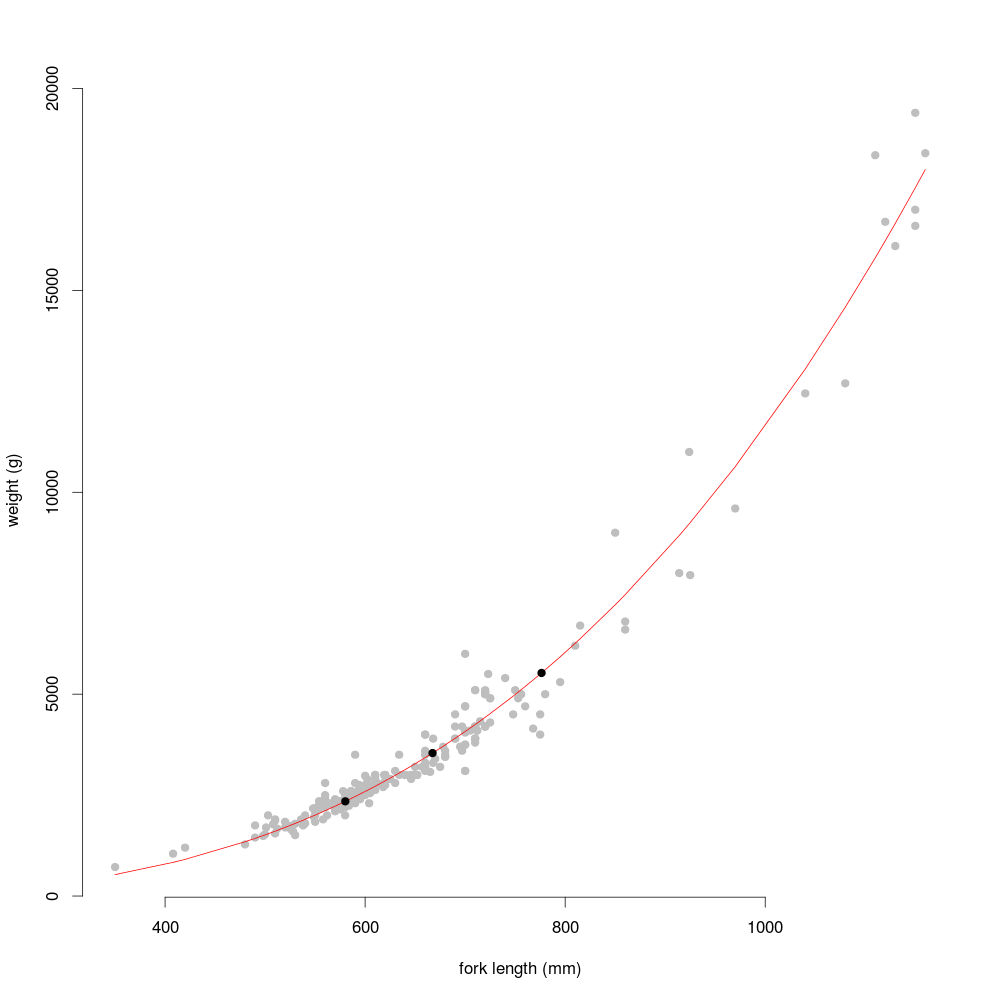
\includegraphics[width=.9\linewidth]{/home/demiurgo/Documents/PhD/Atlantis_Model/model_JFR/MandM/img/wl.vid.png}
       \caption{allometric relationship Vidriola}
       \end{figure}


\begin{itemize}
\item \underline{Whales}

\begin{center}
\begin{tabular}{lrlll}
 Average weight  &  Average (gr)  &  Specie                      &  Common name  &  Source  \\
\hline
 1000 - 3000 kg  &       2000000  &  Globicephala macrorhynchus  &  Pilot Whale  &  NOAA    \\
 13607 - 40823   &      27215000  &  Physeter macrocephalus      &  Sperm Whale  &  NOAA    \\
\hline
 Total Average   &      29215000  &                              &               &          \\
\end{tabular}
\end{center}


\begin{itemize}
\item Reserve weight and structural weight (1 : 2.65)

\begin{verbatim}
library(ascii)
options(asciiType="org")
t.wei <- 29215000
t.wei <- (t.wei / 20) * 1000 ## conversion from g to mg

## From dry weight to nitrogen
t.wei <- t.wei / 5.7

##--------------------------------------------------------------------------
## Generaly the ratio between structural weight and reserve weight is 1:2.65
##  -  -  -  -  -  -  -  -  -  -  -  -  -  -  -  -  -  -  -  -  -  -  -  -  -  -
factor  <- t.wei / 3.65
out     <- data.frame(structural = factor, reserve = factor * 2.65)
cap     <- 'Structural and reserve weight for Whales'
b       <- ascii(out,header=T,  include.rownames = FALSE, include.colnames = T, caption=cap)
print(b)
\end{verbatim}
\end{itemize}
\end{itemize}
=\#+CAPTION: Structural and reserve weight for Whales

\begin{center}
\begin{tabular}{rr}
  structural  &       reserve  \\
\hline
 70211487.62  &  186060442.20  \\
\end{tabular}
\end{center}


=          \#+CAPTION: Structural and reserve weight for Whales

\begin{center}
\begin{tabular}{rr}
  structural  &       reserve  \\
\hline
 70211487.62  &  186060442.20  \\
\end{tabular}
\end{center}



\begin{itemize}
\item \underline{Dophin}

\begin{center}
\begin{tabular}{lrlll}
 Average weight  &  Average (gr)  &  Specie              &  Common name         &  Source  \\
\hline
 300 - 635 kg    &        467500  &  Tursiops truncatus  &  Bottlenose Dolphin  &  NOAA    \\
\end{tabular}
\end{center}



\begin{verbatim}
library(ascii)
options(asciiType="org")
t.wei <- 467500
t.wei <- (t.wei / 20) * 1000 ## conversion from g to mg

## From dry weight to nitrogen
t.wei <- t.wei / 5.7

##--------------------------------------------------------------------------
## Generaly the ratio between structural weight and reserve weight is 1:2.65
##  -  -  -  -  -  -  -  -  -  -  -  -  -  -  -  -  -  -  -  -  -  -  -  -  -  -
factor  <- t.wei / 3.65
out     <- data.frame(structural = factor, reserve = factor * 2.65)
cap     <- 'Structural and reserve weight for Whales'
b       <- ascii(out,header=T,  include.rownames = FALSE, include.colnames = T, caption=cap)
print(b)
\end{verbatim}
\end{itemize}
\begin{table}[htb]
\caption{Structural and reserve weight for Whales}
\begin{center}
\begin{tabular}{rr}
 structural  &     reserve  \\
\hline
 1123528.00  &  2977349.19  \\
\end{tabular}
\end{center}
\end{table}


\begin{itemize}
\item \underline{Birds}

\begin{center}
\begin{tabular}{rrrrl}
  Weight  &  Avera weight (gr)  &  Structural  &  Reserve  &  reference                                                                                                                            \\
\hline
 580-900  &                740  &      202.74  &   537.26  &  \href{http://www.oiseaux-birds.com/card-pink-footed-shearwater.html}{http://www.oiseaux-birds.com/card-pink-footed-shearwater.html}  \\
\end{tabular}
\end{center}




\begin{verbatim}
library(ascii)
options(asciiType="org")
t.wei <- 740
t.wei <- (t.wei / 20) * 1000 ## conversion from g to mg

## From dry weight to nitrogen
t.wei <- t.wei / 5.7

##--------------------------------------------------------------------------
## Generaly the ratio between structural weight and reserve weight is 1:2.65
##  -  -  -  -  -  -  -  -  -  -  -  -  -  -  -  -  -  -  -  -  -  -  -  -  -  -
factor  <- t.wei / 3.65
out     <- data.frame(structural = factor, reserve = factor * 2.65)
cap     <- 'Structural and reserve weight for Birds'
b       <- ascii(out,header=T,  include.rownames = FALSE, include.colnames = T, caption=cap)
print(b)
\end{verbatim}

\begin{center}
\begin{tabular}{rr}
 structural  &  reserve  \\
\hline
    1778.42  &  4712.81  \\
\end{tabular}
\end{center}


\end{itemize}

\end{itemize} % ends low level
\paragraph*{Spatial Cover}
\label{sec-5-2-1-7}

\begin{itemize}
\item For the Cover, I used the data for friedman and also I ude data from Yañez et al.

\begin{verbatim}
## ~~~~~~~~~~~~~~~~~~~~~~~~~~~~~~~~~~~~~~~~~~~~~~~~~~~~~~ ##
## ~              Total Sediment Cover By Box           ~ ##
## ~~~~~~~~~~~~~~~~~~~~~~~~~~~~~~~~~~~~~~~~~~~~~~~~~~~~~~ ##
## Estimation of the total cover by area
source('/home/demiurgo/Documents/PhD/Atlantis_Model/tools/General_tools/Atlantis_tools.R')
library(ascii)
options(asciiType = "org")
# data
lc        <- read.csv('/home/demiurgo/Documents/PhD/Functional_groups/location/Cover/Distribution.csv')
poly      <- read.poly('/home/demiurgo/Documents/PhD/Polygonos/Map/Polygons_20170510.csv')
centroids <- read.csv('/home/demiurgo/Documents/PhD/Functional_groups/location/Cover/centroids.csv')
##~ FUNCTIONAL GROUPS
lc <- FG(data = lc, column = 2)
##~ Weight
lc <- WtoN(lc, 6, 9, 7)
## By season
lc$season.vat <- with(lc,  ifelse(Month %in% c(1, 2, 3), 1,
                           ifelse(Month %in% c(4, 5, 6), 2,
                           ifelse(Month %in% c(7, 8, 9), 3, 4))))
lc <- lc[complete.cases(lc), ] ## removing NaNs
## Relocate the point inside the island to the closest polygons
lon    <- as.matrix(poly$coor[, c(seq(from = 1, to = dim(poly$coor)[2], by = 2))])
lat    <- as.matrix(poly$coor[, c(seq(from = 2, to = dim(poly$coor)[2], by = 2))])
points <- cbind(-lc$Lon, -lc$Lat)
for(island in c(49, 46)){
    is.poly <- na.omit(cbind(lon[order(poly$attrib$box_id), ][island,], lat[order(poly$attrib$box_id), ][island,]))
    points  <- move.point(points, centroids, is.poly)
}
lc$Lon <- -points[, 1]
lc$Lat <- -points[, 2]
## by Groups
lc.FG    <- split(lc, lc$FG)
## poly
poly <- by.pol(poly, lc.FG, la = 5, lo = 4, sea = 11, mult = 10, is.Crus = TRUE)
## Only sumer sampling
loc      <- which(colnames(poly[[1]]$attrib) %in% c("COR", "ROC", "MA", "SAN", "BFF", "BCA"))
sed.type <- poly[[1]]$attrib[, loc]
sed.prop <- sed.type / rowSums(sed.type, na.rm = T)
sed.prop[which(is.na(sed.prop), arr.ind = TRUE)] <- 0
ord      <- order(poly[[1]]$attrib[, 1])
## Save data
out      <- data.frame(box =  poly[[1]]$attrib[ord, 1], sed.prop[ord, ])
write.table(out, '/home/demiurgo/Documents/PhD/Functional_groups/location/Cover/Type.sed.csv', row.names = FALSE)
cap      <- 'Cover by polygon'
b        <- ascii(t(out), header = T,  include.rownames = TRUE, include.colnames = FALSE, caption=cap, digits=3)
print(b)
\end{verbatim}

\begin{center}
\begin{tabular}{lrrrrrrrrrrrrrrrrrrrrrrrrrrrrrrrrrrrrrrrrrrrrrrrrrrrrrrrrrrr}
 box  &  0.000  &  1.000  &  2.000  &  3.000  &  4.000  &  5.000  &  6.000  &  7.000  &  8.000  &  9.000  &  10.000  &  11.000  &  12.000  &  13.000  &  14.000  &  15.000  &  16.000  &  17.000  &  18.000  &  19.000  &  20.000  &  21.000  &  22.000  &  23.000  &  24.000  &  25.000  &  26.000  &  27.000  &  28.000  &  29.000  &  30.000  &  31.000  &  32.000  &  33.000  &  34.000  &  35.000  &  36.000  &  37.000  &  38.000  &  39.000  &  40.000  &  41.000  &  42.000  &  43.000  &  44.000  &  45.000  &  46.000  &  47.000  &  48.000  &  49.000  &  50.000  &  51.000  &  52.000  &  53.000  &  54.000  &  55.000  &  56.000  &  57.000  &  58.000  \\
\hline
 BCA  &  0.000  &  0.000  &  0.000  &  0.000  &  0.000  &  0.000  &  0.000  &  0.000  &  0.000  &  0.000  &   0.000  &   0.000  &   0.000  &   0.000  &   0.000  &   0.000  &   0.000  &   0.000  &   0.000  &   0.000  &   0.000  &   0.000  &   0.000  &   0.000  &   0.000  &   0.000  &   0.333  &   0.000  &   0.000  &   0.000  &   0.000  &   0.000  &   0.000  &   0.000  &   1.000  &   1.000  &   1.000  &   1.000  &   0.000  &   0.000  &   0.000  &   0.000  &   0.000  &   1.000  &   0.000  &   0.000  &   0.000  &   0.000  &   0.000  &   0.000  &   0.000  &   0.031  &   0.031  &   0.037  &   0.041  &   0.016  &   0.043  &   0.474  &   0.419  \\
 BFF  &  0.000  &  0.000  &  0.000  &  0.000  &  0.000  &  0.000  &  0.000  &  0.000  &  0.000  &  0.000  &   0.000  &   0.000  &   0.000  &   0.000  &   0.000  &   0.000  &   0.000  &   0.000  &   0.000  &   0.000  &   0.000  &   0.000  &   0.000  &   0.000  &   0.000  &   0.000  &   0.000  &   0.000  &   0.000  &   0.000  &   0.000  &   0.000  &   0.000  &   0.000  &   0.000  &   0.000  &   0.000  &   0.000  &   0.000  &   0.000  &   0.000  &   0.000  &   0.000  &   0.000  &   0.000  &   0.000  &   0.000  &   0.000  &   0.000  &   0.000  &   0.000  &   0.262  &   0.253  &   0.109  &   0.260  &   0.025  &   0.000  &   0.526  &   0.581  \\
 COR  &  0.000  &  0.000  &  0.000  &  0.000  &  0.000  &  0.000  &  0.000  &  0.000  &  0.000  &  0.000  &   0.000  &   0.000  &   0.000  &   0.000  &   0.000  &   0.000  &   0.000  &   0.000  &   0.000  &   0.000  &   0.000  &   0.000  &   0.000  &   0.000  &   0.000  &   0.000  &   0.667  &   0.000  &   0.000  &   0.000  &   0.000  &   0.000  &   0.000  &   0.000  &   0.000  &   0.000  &   0.000  &   0.000  &   0.000  &   0.000  &   0.000  &   0.000  &   0.000  &   0.000  &   0.000  &   0.000  &   0.000  &   0.000  &   0.000  &   0.000  &   0.000  &   0.059  &   0.060  &   0.085  &   0.055  &   0.958  &   0.957  &   0.000  &   0.000  \\
 MA   &  0.000  &  0.000  &  0.000  &  0.000  &  0.000  &  0.000  &  0.000  &  0.000  &  0.000  &  0.000  &   0.000  &   0.000  &   0.000  &   0.000  &   0.000  &   0.000  &   0.000  &   0.000  &   0.000  &   0.000  &   0.000  &   0.000  &   0.000  &   0.000  &   0.000  &   0.000  &   0.000  &   0.000  &   0.000  &   0.000  &   0.000  &   0.000  &   0.000  &   0.000  &   0.000  &   0.000  &   0.000  &   0.000  &   0.000  &   0.000  &   0.000  &   0.000  &   0.000  &   0.000  &   0.000  &   0.000  &   0.000  &   0.000  &   0.000  &   0.000  &   0.000  &   0.569  &   0.577  &   0.676  &   0.566  &   0.000  &   0.000  &   0.000  &   0.000  \\
 ROC  &  0.000  &  0.000  &  0.000  &  0.000  &  0.000  &  0.000  &  0.000  &  0.000  &  0.000  &  0.000  &   0.000  &   0.000  &   0.000  &   0.000  &   0.000  &   0.000  &   0.000  &   0.000  &   0.000  &   0.000  &   0.000  &   0.000  &   0.000  &   0.000  &   0.000  &   0.000  &   0.000  &   0.000  &   0.000  &   0.000  &   0.000  &   0.000  &   0.000  &   0.000  &   0.000  &   0.000  &   0.000  &   0.000  &   0.000  &   0.000  &   0.000  &   0.000  &   0.000  &   0.000  &   0.000  &   0.000  &   0.000  &   0.000  &   0.000  &   0.000  &   0.000  &   0.059  &   0.060  &   0.070  &   0.059  &   0.000  &   0.000  &   0.000  &   0.000  \\
 SAN  &  0.000  &  0.000  &  0.000  &  0.000  &  0.000  &  0.000  &  0.000  &  0.000  &  0.000  &  0.000  &   0.000  &   0.000  &   0.000  &   0.000  &   0.000  &   0.000  &   0.000  &   0.000  &   0.000  &   0.000  &   0.000  &   0.000  &   0.000  &   0.000  &   0.000  &   0.000  &   0.000  &   0.000  &   0.000  &   0.000  &   0.000  &   0.000  &   0.000  &   0.000  &   0.000  &   0.000  &   0.000  &   0.000  &   0.000  &   0.000  &   0.000  &   0.000  &   0.000  &   0.000  &   0.000  &   0.000  &   0.000  &   0.000  &   0.000  &   0.000  &   0.000  &   0.020  &   0.020  &   0.023  &   0.020  &   0.000  &   0.000  &   0.000  &   0.000  \\
\end{tabular}
\end{center}


\end{itemize}
\paragraph*{Throphic relation}
\label{sec-5-2-1-8}
\begin{itemize}

\item Availability matrix
\label{sec-5-2-1-8-1}%
\begin{itemize}
\item I will leave this one for the last part
\item Gape size
    I will use the normal limits (0.1\% to 40\%)
\item I increase the value of KLP to 1e-06 for whales
\end{itemize}

\item Estimation of structural weight to calculate the biomass for predation\\
\label{sec-5-2-1-8-2}%
\begin{verbatim}
source('/home/demiurgo/Documents/PhD/Atlantis_Model/tools/General_tools/Atlantis_tools.R')
library(ascii)
options(asciiType="org")
data  <- read.csv('/home/demiurgo/Documents/PhD/Functional_groups/Structural_weight/SN.csv')
out   <- with(data, weights(FG, weight, metric = 'g'))
cap   <- 'Structural and reserve weight for all the biomass GF'
b     <- ascii(out,header=T,  include.rownames = FALSE, include.colnames = T, caption=cap)
print(b)
\end{verbatim}

\begin{center}
\begin{tabular}{lrr}
 Functional_Groups  &   structural  &       reserve  \\
\hline
 CHO                &     11103.10  &      29423.22  \\
 OTA                &    225907.23  &     598654.17  \\
 CET                &  70211487.62  &  186060442.20  \\
 BIR                &      1778.42  &       4712.81  \\
 OCT                &      1737.56  &       4604.54  \\
 SCR                &      1485.22  &       3935.83  \\
 BFF                &       240.33  &        636.87  \\
 BCA                &       456.44  &       1209.57  \\
 MOL                &       672.92  &       1783.23  \\
 DOL                &   1123528.00  &    2977349.19  \\
 MPF                &        81.71  &        216.53  \\
\end{tabular}
\end{center}




\item Estimation of Clearance\\
\label{sec-5-2-1-8-3}%
I use the length of the individual and the speed of each one,  there is another aproximation but I need to have the production and the number of preys. In this aproximation,  I asume that the clearence rate is equal to the time and the speed looking for food.

\begin{verbatim}
library(ascii)
library(ggplot2)
source('/home/demiurgo/Documents/PhD/Atlantis_Model/tools/General_tools/Atlantis_tools.R')
options(asciiType = "org")
data <- read.csv('/home/demiurgo/Documents/PhD/Functional_groups/Clearance/c_data.csv')
## swimming speed
## from mm to  meters
data$length <- data$length  / 1000
cap         <- 'Clearance by cohort for some functional groups [m3d-1]'
C.out       <- clearance(fg        = data[, 1],
                         speed     = data[, 3],
                         len       = data[, 2],
                         ratio     = data[, 4],
                         time.l    = data[, 5],
                         max.speed = data[, 6],
                         alfa      = data[, 7],
                         beta      = data[, 8],
                         height    = data[, 9])
p.C <- C.out
p.C   <- na.omit(data.frame(FG= rownames(p.C), Cohort = sort(rep(1 : 10, nrow(p.C))), Clearance = c(p.C)))
png('img/clearance.png', height = 1000, width = 1000)
sp    <- ggplot(data=p.C, aes(Cohort, Clearance))+ geom_line()
sp + facet_wrap(~FG, ncol = 4, scales = 'free_y')
invisible(dev.off())
b     <- ascii(C.out,header=T,  include.rownames = TRUE, include.colnames = TRUE, caption=cap)
print(b)
\end{verbatim}

\begin{center}
\begin{tabular}{lrrrrrrrrrr}
      &       1  &       2  &       3  &       4  &       5  &       6  &       7  &       8  &       9  &      10  \\
\hline
 ALF  &   60.63  &  103.65  &  162.00  &  220.38  &  275.70  &  326.34  &  371.68  &  411.51  &  446.29  &  476.03  \\
 ANG  &    2.35  &    5.40  &   15.31  &   27.69  &   41.03  &   54.57  &   67.63  &   79.87  &   91.07  &   79.94  \\
 BIR  &    0.41  &    2.18  &    5.28  &    9.24  &   13.61  &   18.04  &   22.28  &   26.20  &   29.72  &   32.81  \\
 BRC  &    6.48  &   10.71  &   16.42  &   23.56  &   32.69  &   45.00  &   60.26  &   74.35  &   88.78  &  104.92  \\
 CHO  &    1.46  &    4.65  &    8.43  &   12.19  &   15.63  &   18.64  &   21.19  &   23.31  &   25.05  &   26.46  \\
 DOL  &    8.61  &   28.21  &   52.40  &   77.46  &  101.36  &  123.08  &  142.24  &  158.78  &  172.86  &  184.71  \\
 GCR  &    0.52  &    1.74  &    3.65  &    6.16  &    9.14  &   12.25  &   15.07  &   17.38  &   19.85  &   22.03  \\
 LBF  &   91.93  &  113.55  &  141.53  &  163.87  &  191.05  &  235.31  &  272.21  &  295.86  &  331.94  &  370.96  \\
 LPF  &   14.39  &  101.53  &  172.50  &  213.82  &  235.53  &  246.48  &  251.90  &  254.56  &  255.86  &  256.49  \\
 MPF  &    9.81  &   13.06  &   13.66  &   13.76  &   13.78  &   13.78  &          &          &          &          \\
 ORO  &    3.24  &   20.25  &   39.76  &   56.91  &   68.62  &   76.15  &   80.84  &   83.71  &   85.43  &   86.47  \\
 OTA  &  175.96  &  242.84  &  300.52  &  348.19  &  386.54  &  416.85  &  440.52  &  458.85  &  472.94  &  483.74  \\
 SBF  &   47.94  &   71.63  &  100.05  &  141.74  &  188.87  &  256.62  &  300.12  &  406.55  &  475.32  &  549.46  \\
 SPF  &   10.15  &   46.63  &  100.30  &  149.76  &  190.13  &  221.14  &  244.16  &  260.90  &  272.91  &  281.44  \\
 SPL  &    1.90  &    2.28  &    2.70  &    3.15  &    3.71  &    4.18  &    4.67  &    5.10  &    5.56  &    6.03  \\
 VID  &   67.01  &   88.68  &  120.00  &          &          &          &          &          &          &          \\
\end{tabular}
\end{center}


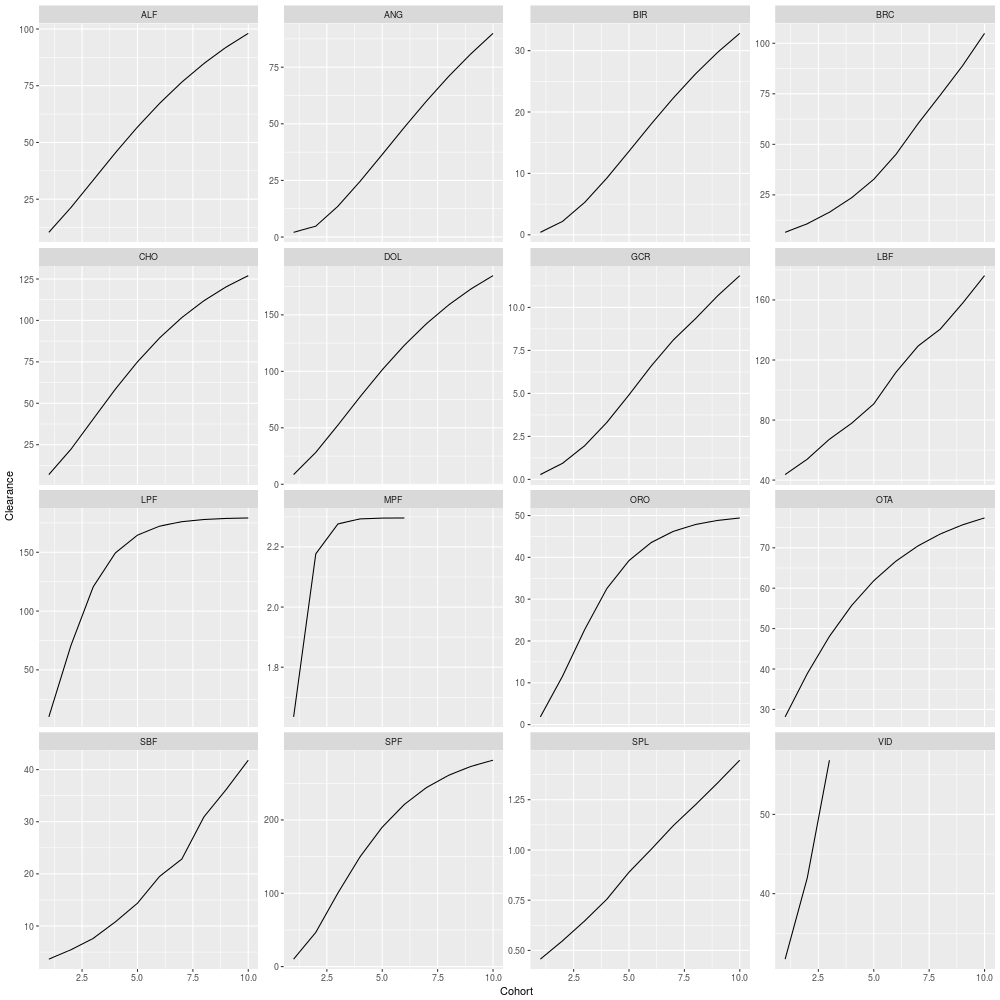
\includegraphics[width=.9\linewidth]{/home/demiurgo/Documents/PhD/Atlantis_Model/model_JFR/MandM/img/clearance.png}


\item Estimation of growth rate
\label{sec-5-2-1-8-4}%
\begin{itemize}
\item First, I estimated the value of the alfa and beta parameters from the allometric relationship

\begin{verbatim}
## ~~~~~~~~~~~~~~~~~~~~~~~~~~~~~~~~~~~~~~~~~~~~~~~~~~~~~~~~~~~~~~~~~~~~~~~~~~ ##
## ~                   estimation length weight relationship                ~ ##
## ~~~~~~~~~~~~~~~~~~~~~~~~~~~~~~~~~~~~~~~~~~~~~~~~~~~~~~~~~~~~~~~~~~~~~~~~~~ ##
library(ascii)
options(asciiType="org")
source('/home/demiurgo/Documents/PhD/Atlantis_Model/tools/General_tools/Atlantis_tools.R')
spgrey <- rgb(t(col2rgb("black")), alpha=30, maxColorValue=255)
## read the data
dat    <- read.csv("/home/demiurgo/Documents/PhD/Functional_groups/length_weight/length_weight_jf.csv")
## Grupos funcionales
lf          <- FG(dat, 2)
## The length is in mm. So it needed to changed to cm
lf[, 3 : 4] <- lf[, 3 : 4] / 10
##-----------
##  Divide by functional group
##---------------
lf.fg       <- split(lf, lf$FG)  # split by functional group
## type of length that I used in the estimation of the cohorts for each functional group
len.ty <- c('total','total', 'total', 'total', 'total', 'fork',
            'total', 'total', 'total','total','total', 'total','fork', 'total', 'total')
alometric <- function(length, alfa, beta){
    weight <- alfa  * length ^ beta
    return(weight)
}
## information from Fishbase The values on the data base are not reliable
cho <- c(alfa=0.00210, beta=3.176)
## Due to the lack of information I will remove some groups
## Removing octopus
lf.fg <- lf.fg[ - 9]
png('img/allometric.png', width = 1200, height = 900)
res <- list()
par(mfrow=c(3, 5), mar = c(4, 2, 1, 2), oma=c(3, 2, 0, 2), cex = 1.2)
    for(i in 1:length(lf.fg)){
    len       <- lf.fg[[i]][, ifelse(len.ty[i] == 'total', 4, 3)]
    weight    <- lf.fg[[i]][, 5]
    ## orden the list,  jut for plotting
    or        <- order(len)
    len       <- len[or]
    weight    <- weight[or]
    res[[i]]  <- nls(weight~alometric(len, alfa, beta), start = c(alfa = 0.5, beta = ifelse(i%in%c(4,1,9), 3, 1.4)),
                     trace = FALSE, control = nls.control(maxiter = 5000, minFactor = 1/100000))
    plot(len, weight, col = spgrey, pch = 20, bty = 'n', xlab = '', ylab = '', main = lf.fg[[i]]$FG[1] )
    lines(len[!is.na(len)], predict(res[[i]]), col = 2)
    if(i == 4) lines(len[!is.na(len)], alometric(len[!is.na(len)], cho[1],cho[2]), col=4)
    if( i == 1){
        parameters <- coef(res[[i]])
    } else if(i == 4){
        parameters <- cbind(parameters, cho)
    } else {
        parameters <- cbind(parameters, coef(res[[i]]))
    }
}
mtext(text="Weight (gr)",side=2,outer=TRUE,font=2,cex=1.5)
mtext(text="Length (cm)",side=1,outer=TRUE,font=2,cex=1.5)
invisible(dev.off())
## table with parameters
cap                  <- 'Values of the paramter alfa and beta in the allometric relationship for each functional group'
colnames(parameters) <- names(lf.fg)
b                    <- ascii(parameters, header=T,  include.rownames = TRUE, include.colnames = T, caption = cap, digit = 8)
print(b)
\end{verbatim}

\begin{center}
\begin{tabular}{lrrrrrrrrrrrrrr}
       &         ALF  &         ANG  &         BRC  &         CET  &           CHO  &         GCR  &         LBF  &         LPF  &         ORO  &         OTA  &         SBF  &         SPF  &         SPL  &         VID  \\
\hline
 alfa  &  0.07147389  &  0.00470168  &  0.00419986  &  0.00210000  &  164.38180473  &  0.53179259  &  0.00023791  &  0.06825499  &  0.06883698  &  3.88353881  &  1.57860495  &  0.00716116  &  0.96225457  &  0.00523585  \\
 beta  &  2.70714831  &  2.83452053  &  3.21196191  &  3.17600000  &    0.78557000  &  2.84013419  &  3.89821853  &  2.50292955  &  2.70895066  &  2.07274350  &  1.77322880  &  3.14316080  &  2.71901358  &  3.10821550  \\
\end{tabular}
\end{center}


    \begin{figure}[htb]
    \centering
    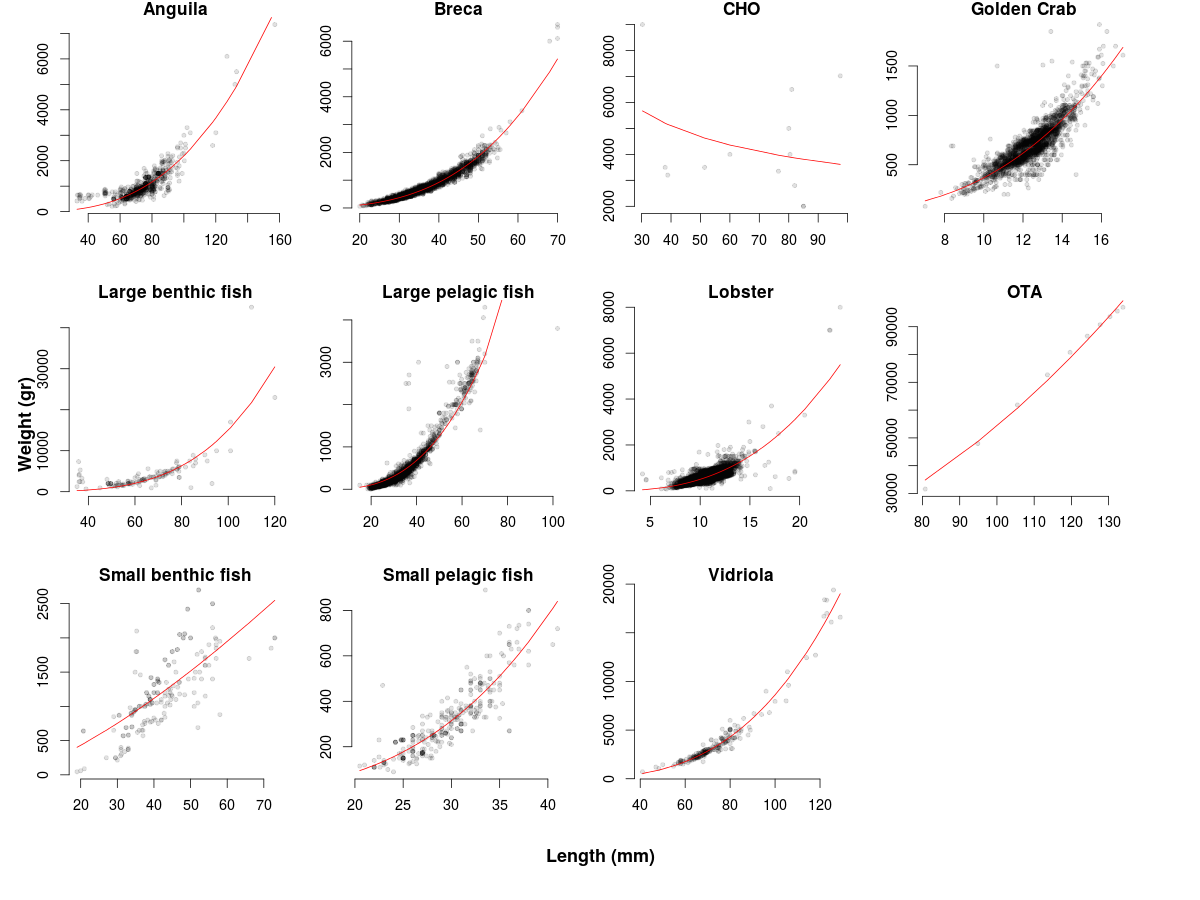
\includegraphics[width=.9\linewidth]{/home/demiurgo/Documents/PhD/Atlantis_Model/model_JFR/MandM/img/allometric.png}
    \caption{Allometric relationship for different functional groups}
    \end{figure}
\item For Seals I use the values from Amano2000
\begin{itemize}
\item \( W = 71.6(1 - 0.323 * exp( - 0.248 * t))^3 \)
\end{itemize}
\item Estimation of Alometric relationship for the length on meters

\begin{verbatim}
## ~~~~~~~~~~~~~~~~~~~~~~~~~~~~~~~~~~~~~~~~~~~~~~~~~~~~~~~~~~~~~~~~~~~~~~~~~~ ##
## ~                   estimation length weight relationship                ~ ##
## ~~~~~~~~~~~~~~~~~~~~~~~~~~~~~~~~~~~~~~~~~~~~~~~~~~~~~~~~~~~~~~~~~~~~~~~~~~ ##
library(ascii)
options(asciiType="org")
source('/home/demiurgo/Documents/PhD/Atlantis_Model/tools/General_tools/Atlantis_tools.R')
spgrey <- rgb(t(col2rgb("black")), alpha=30, maxColorValue=255)
## read the data
dat    <- read.csv("/home/demiurgo/Documents/PhD/Functional_groups/length_weight/length_weight_jf.csv")
## Grupos funcionales
lf          <- FG(dat, 2)
## The length is in mm. So it needed to changed to cm
lf[, 3 : 4] <- lf[, 3 : 4] / 10
##-----------
##  Divide by functional group
##---------------
lf.fg       <- split(lf, lf$FG)  # split by functional group
## type of length that I used in the estimation of the cohorts for each functional group
len.ty <- c('total', 'fork', 'total', 'total', 'fork',
            'total', 'total', 'total', 'total', 'total','fork', 'total', 'total')
alometric <- function(length, alfa, beta){
    weight <- alfa  * length ^ beta
    return(weight)
}
## Removing octopus
lf.fg <- lf.fg[ - 8]
png('img/allometric.png', width = 1200, height = 900)
res <- list()
par(mfrow=c(3, 4), mar = c(4, 2, 1, 2), oma=c(3, 2, 0, 2), cex = 1.2)
for(i in 1:length(lf.fg)){
    len       <- lf.fg[[i]][, ifelse(len.ty[i] == 'total', 4, 3)]
    weight    <- lf.fg[[i]][, 5]
    ## orden the list,  jut for plotting
    or        <- order(len)
    len       <- len[or]
    weight    <- weight[or]
    res[[i]]  <- nls(weight~alometric(len, alfa, beta), start = c(alfa = 0.5, beta = ifelse(i==3, 3, 1.4)),
                     trace = FALSE, control = nls.control(maxiter = 5000, minFactor = 1/100000))
    plot(len, weight, col = spgrey, pch = 20, bty = 'n', xlab = '', ylab = '', main = lf.fg[[i]]$FG[1] )
    lines(len[!is.na(len)], predict(res[[i]]), col = 2)
    if( i == 1){
        parameters <- coef(res[[i]])
    } else {
        parameters <- cbind(parameters, coef(res[[i]]))
    }
}
mtext(text="Weight (gr)",side=2,outer=TRUE,font=2,cex=1.5)
mtext(text="Length (cm)",side=1,outer=TRUE,font=2,cex=1.5)
invisible(dev.off())
## table with parameters
cap                  <- 'Values of the paramter alfa and beta in the allometric relationship for each functional group'
colnames(parameters) <- names(lf.fg)
b                    <- ascii(parameters, header=T,  include.rownames = TRUE, include.colnames = T, caption = cap, digit = 8)
print(b)
\end{verbatim}

\begin{center}
\begin{tabular}{lrrrrrrrrrrrr}
       &         ANG  &         BRC  &         CET  &           CHO  &         GCR  &         LBF  &         LPF  &         OTA  &         SBF  &         SPF  &         SPL  &         VID  \\
\hline
 alfa  &  0.00470168  &  0.00839310  &  0.01787816  &  164.38180473  &  0.53179259  &  0.00023791  &  0.06825499  &  3.88353881  &  1.57860495  &  0.00716116  &  0.96225457  &  0.00523585  \\
 beta  &  2.83452053  &  3.14636532  &  2.92615017  &    0.78557000  &  2.84013419  &  3.89821853  &  2.50292955  &  2.07274350  &  1.77322880  &  3.14316080  &  2.71901358  &  3.10821550  \\
\end{tabular}
\end{center}


    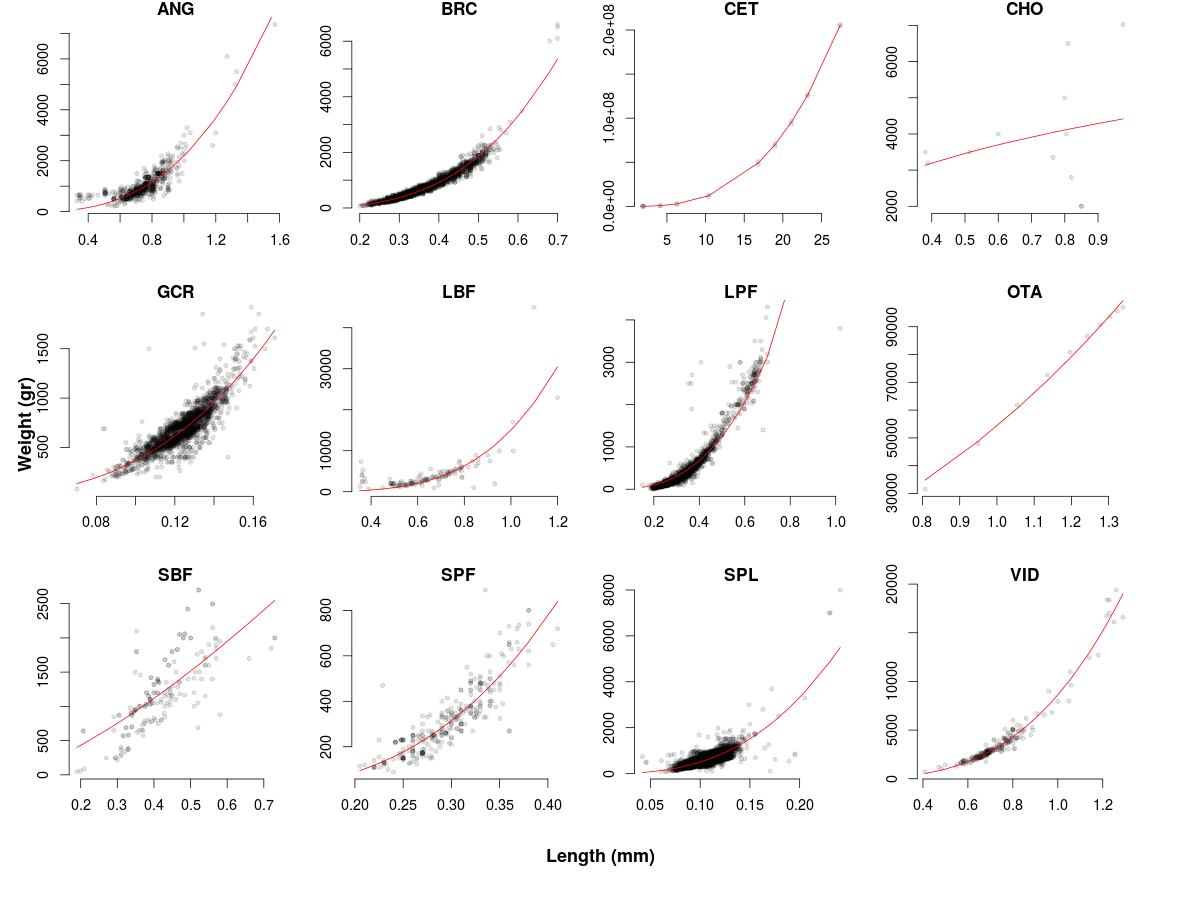
\includegraphics[width=.9\linewidth]{/home/demiurgo/Documents/PhD/Atlantis_Model/model_JFR/MandM/img/allometric_meter.png}
\item Calculation of mum

\begin{verbatim}
## ~~~~~~~~~~~~~~~~~~~~~~~~~~~~~~~~~~ ##
## ~         Estimation of mum      ~ ##
## ~~~~~~~~~~~~~~~~~~~~~~~~~~~~~~~~~~ ##
data  <- read.csv('/home/demiurgo/Documents/PhD/Functional_groups/mum/mum.csv')
library(ascii)
library(ggplot2)
options(asciiType="org")
source('/home/demiurgo/Documents/PhD/Atlantis_Model/tools/General_tools/Atlantis_tools.R')
## estimation of the weight at each age class or cohort
data$Weight <- ifelse(is.na(data$Weight), alometric(data$Length, data$alfa, data$beta), data$Weight)
fg          <- split(data, data$FG)
spw.rate    <- 1.2
res         <- list()
for( i in 1: length(fg)) {
    res[[i]] <- with(fg[[i]], mum.f(length     = Length,   # Length in cm
                                    weight     = Weight,   # Weight
                                    metric     = 'g',      # metric for weight grams
                                    spw.rate   = 1.4,      # I asume that 40% of the reserve weight in going to reproduction
                                    mature     = Mature,   # Age at maturity
                                    AgeClass   = AgeClass))# Number year for earch Age class
}
## Arrangement for the output
m   <- as.vector(table(data[, 1]))
out <- matrix(NA, nrow = max(m), ncol = length(m))
dat <- array()
for(i in 1 : length(res)){
    out[, i] <- c(res[[i]], rep(NA, 10 - length(res[[i]])))
    if(length(res[[i]]) > 1){
        dat <- rbind(dat, cbind(rep(names(fg)[i], length(res[[i]])),res[[i]], seq(1 : length(res[[i]]))))
    }
}
dat           <- data.frame(FG = dat[-1, 1], Mum = as.numeric(dat[-1, 2]), Age = as.numeric(dat[-1, 3]))
out           <- t(out)
rownames(out) <- names(fg)
colnames(out) <- c(1 : (ncol(out)))
sp            <- ggplot(data=dat, aes(Age, Mum))+ geom_line()
png('img/mum.png', height = 1200, width = 1200)
sp + facet_wrap(~FG, ncol=4, scales = 'free_y')
invisible(dev.off())
## table with parameters
cap                  <- 'Values of growth rate (mum) for each functional group [mgN-1d-1]'
b                    <- ascii(out, header=T,  include.rownames = TRUE, include.colnames = T, caption = cap, digits = 3)
cat("#+ATTR_HTML: :style float:left;width:30%;margin:3ex\n")
print(b)
\end{verbatim}
\begin{table}[htb]
\caption{Values of growth rate (mum) for each functional group [mgN-1d-1]}
\begin{center}
\begin{tabular}{lrrrrrrrrrr}
      &      1  &      2  &       3  &       4  &       5  &        6  &       7  &       8  &        9  &       10  \\
\hline
 ALF  &  0.083  &  0.342  &   1.058  &   1.707  &   2.517  &    3.511  &   4.713  &   6.172  &    7.903  &   10.063  \\
 ANG  &  0.001  &  0.013  &   0.081  &   0.181  &   0.319  &    0.494  &   0.710  &   0.970  &    1.282  &    1.652  \\
 BCA  &  0.464  &         &          &          &          &           &          &          &           &           \\
 BFF  &  0.061  &         &          &          &          &           &          &          &           &           \\
 BIR  &  0.023  &  0.211  &   0.539  &   1.008  &   1.619  &    2.386  &   3.332  &   4.491  &    5.905  &    7.629  \\
 BRC  &  0.046  &  0.178  &   0.520  &   0.750  &   1.015  &    1.310  &   1.722  &   2.484  &    3.183  &    3.764  \\
 CHO  &  0.016  &  0.106  &   0.418  &   0.796  &   1.294  &    1.928  &   2.727  &   3.732  &    4.999  &    6.597  \\
 DOL  &  0.079  &  0.676  &   1.678  &   3.077  &   4.883  &    7.143  &   9.938  &  13.376  &   17.602  &   22.797  \\
 GCR  &  0.011  &  0.058  &   0.213  &   0.408  &   0.677  &    1.039  &   1.541  &   2.239  &    2.653  &    3.471  \\
 LBF  &  0.120  &  0.548  &   0.749  &   2.540  &   3.082  &    3.468  &   5.320  &   8.782  &    8.274  &    9.952  \\
 LPF  &  0.021  &  0.189  &   0.508  &   0.981  &   1.839  &    3.542  &   7.010  &  14.120  &   28.721  &   58.714  \\
 MOL  &  0.684  &         &          &          &          &           &          &          &           &           \\
 MPF  &  0.052  &  0.494  &   2.071  &  11.434  &  68.050  &  410.553  &          &          &           &           \\
 OCT  &  0.353  &         &          &          &          &           &          &          &           &           \\
 ORO  &  0.001  &  0.039  &   0.143  &   0.239  &   0.826  &    1.360  &   2.220  &   3.629  &    6.039  &   10.026  \\
 OTA  &  2.276  &  6.748  &  21.073  &  28.824  &  38.571  &   51.143  &  67.582  &  89.225  &  117.806  &  155.600  \\
 SBF  &  0.129  &  0.248  &   0.730  &   0.815  &   1.022  &    1.106  &   1.840  &   1.329  &    2.201  &    2.462  \\
 SCR  &  1.258  &         &          &          &          &           &          &          &           &           \\
 SPF  &  0.014  &  0.126  &   0.581  &   1.233  &   2.113  &    3.295  &   4.911  &   7.163  &   10.342  &   14.860  \\
 SPL  &  0.127  &  0.374  &   1.292  &   1.556  &   1.717  &    2.357  &   2.747  &   3.513  &    3.908  &    4.330  \\
 VID  &  0.239  &  1.847  &   2.435  &          &          &           &          &          &           &           \\
\end{tabular}
\end{center}
\end{table}


    \begin{figure}[htb]
    \centering
    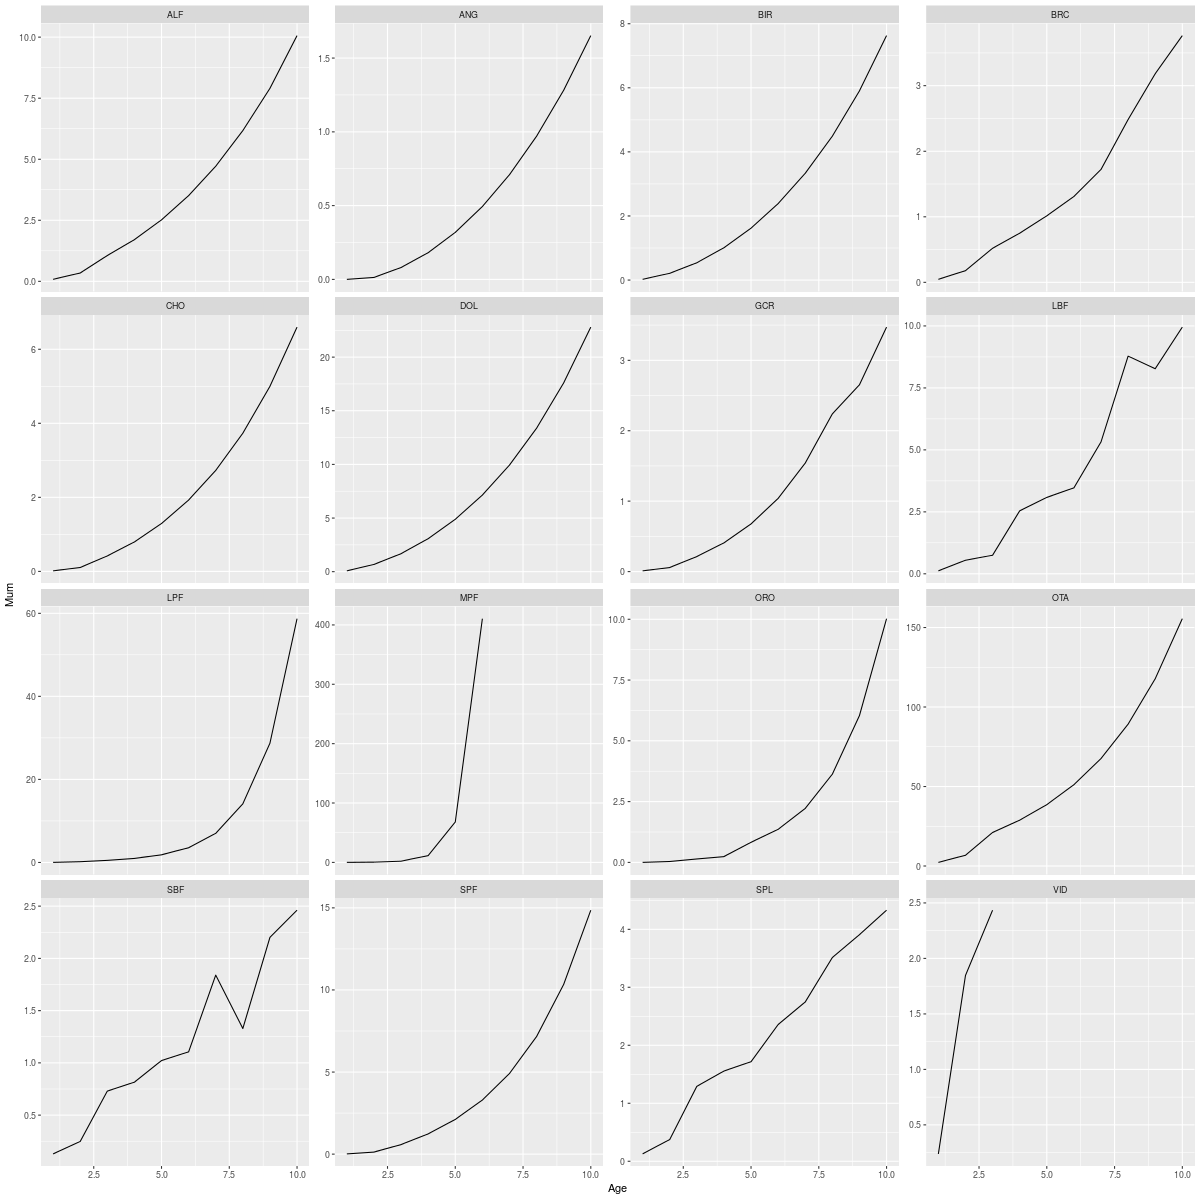
\includegraphics[width=.9\linewidth]{img/mum.png}
    \caption{Values of Growth rate for each Vertebrate Functional Group}
    \end{figure}
\end{itemize}

\item Maturity and Spawning
\label{sec-5-2-1-8-5}%
\begin{table}[htb]
\caption{length (in mm) for the reproductive maturity for vertebraes and mobile bentos (with age classes)}
\begin{center}
\begin{tabular}{lrrll}
 FG   &  Maturity  &  Age (y)  &  Reference                         &  Specie                                             \\
\hline
 SPL  &      73.2  &        6  &  Ernst 2013                        &                                                     \\
 GCR  &     10.62  &        6  &  Ernst 2013 \& Canales 2009        &                                                     \\
 BRC  &      28.9  &        5  &  Rivara 2013  \& Hernandez 2012    &                                                     \\
 VID  &        51  &           &  Fishbase                          &  Seriola lalandi                                    \\
 ORO  &        35  &       33  &  Niklischek 2005                   &                                                     \\
 ALF  &      33.2  &        6  &  Wiff 2013 \                       &                                                     \\
 SPF  &        27  &           &  Fishbase                          &  Neoscorpis lithophilus                             \\
 LBF  &        92  &       12  &  Flores \& Rojas 1985 \& Fishbase  &                                                     \\
 ANG  &      43.7  &        2  &  Fishbase                          &                                                     \\
 CHO  &      77.8  &           &  Fishbase                          &  Squalus mitsukurii                                 \\
 OTA  &       105  &        5  &  Amano2000 and Osman               &                                                     \\
 LPF  &      34.5  &        3  &  Fishbase (average)                &  Pseudocaranx dentex                                \\
 SBF  &        21  &           &  Fishbase  + Munoz                 &  Helicolemus dactylipterus  + Girella tricuspidata  \\
 MPF  &       5.6  &        1  &  Fishbase                          &                                                     \\
\end{tabular}
\end{center}
\end{table}


\begin{table}[htb]
\caption{Age of the behavioral maturity for vertebrates and mobile benthos. The age correspond to the cohort}
\begin{center}
\begin{tabular}{lrll}
 Functional Group  &  Maturity  &  Reference             &  Specie                                             \\
\hline
 SPL               &         3  &  Ernst 2013            &                                                     \\
 GCR               &         2  &  Ernst 2013            &                                                     \\
 BRC               &         3  &  Rivara 2013           &                                                     \\
 VID               &         1  &  Fishbase              &  Seriola lalandi                                    \\
 ORO               &         5  &  Niklischek 2005       &                                                     \\
 ALF               &         3  &  Wiff 2013             &                                                     \\
 SPF               &         3  &  Fishbase              &  Neoscorpis lithophilus                             \\
 LBF               &         4  &  Flores \& Rojas 1985  &                                                     \\
 ANG               &         3  &  Fishbase              &                                                     \\
 OTA               &         3  &  Amano2000 and Osman   &                                                     \\
 LPF               &         2  &  Fishbase (average)    &  Pseudocaranx dentex                                \\
 SBF               &         3  &  Fishbase  + Munoz     &  Helicolemus dactylipterus  + Girella tricuspidata  \\
 MPF               &         1  &  Fishbase              &                                                     \\
\end{tabular}
\end{center}
\end{table}


\begin{itemize}
\item Estimation of KSPA$_{\mathrm{XXX}}$ and FSP$_{\mathrm{XXX}}$
    The approach if dereved from the growth function :
\begin{itemize}
\item \(Nr_{S, R} = p_{r}(W_{S} - cr / pr) - min{0, W(s) - (S + R)}\)
\item \(cr / pr = Nm\) \#\# weight just before the maturity age
\item \(pr = {alfa * Nt}/{(1 + alfa) * Nt - Nm}\)
\item \(cr = Nm*pr\)
\item pr = FSP$_{\mathrm{XXX}}$ \& cr = KASP$_{\mathrm{XXX}}$

\begin{verbatim}
## ~~~~~~~~~~~~~~~~~~~~~~~~~~~~~~~~~~~~~~~~~~~~~~~~~~~~~~~~~~~~~~~~~~ ##
## ~                 Estimation of KSPA_XX and FSP_XXX              ~ ##
## ~~~~~~~~~~~~~~~~~~~~~~~~~~~~~~~~~~~~~~~~~~~~~~~~~~~~~~~~~~~~~~~~~~ ##
library(ascii)
options(asciiType = "org")
source('/home/demiurgo/Documents/PhD/Atlantis_Model/tools/General_tools/Atlantis_tools.R')
##read the data
data             <- read.csv('/home/demiurgo/Documents/PhD/Functional_groups/Mature_Growth/Mgrowth.csv')
## getting the weight before reproduction and the weith in equilibrium for all the FG
data$Weight      <- ifelse(is.na(data$Weight), alometric(data$Length, data$Alfa, data$Beta), data$Weight)
data$Weight_equi <- ifelse(is.na(data$Weight_equi), alometric(data$Length2, data$Alfa, data$Beta), data$Weight_equi)
## The weith in mgN for
##~~~ cr/pr == Nm
data$Nm <- weight2N(weight = data$Weight, metric = 'g')
##~~~ Nt = Wigth at equilibrium
data$Nt <- weight2N(weight = data$Weight_equi, metric = 'g')
## Getting KSPA_XXX and FSP_XXX
rate       <- 0.4  # 20% of increase weight durint reproduction
data$FSP   <- with(data, (rate * Nt)/((1 + rate) * Nt - Nm))
data$KSPA  <- with(data, Nm * FSP)
cap        <- 'Values of KASP and FSP for each functional group'
## table with parameters
cap                  <- 'Values of KSPA_XX and FSP_XXX for each functional group'
b                    <- ascii(data, header=T,  include.rownames = FALSE, include.colnames = T, caption = cap)
print(b)
\end{verbatim}
\end{itemize}
\begin{table}[htb]
\caption{Values of KSPA$_{\mathrm{XX}}$ and FSP$_{\mathrm{XXX}}$ for each functional group}
\begin{center}
\begin{tabular}{lrrrrrrrrrr}
 FG   &  Length  &  Length2  &    Weight  &  Weight_equi  &  Alfa  &  Beta  &         Nm  &         Nt  &   FSP  &      KSPA  \\
\hline
 ALF  &   25.58  &    54.82  &    473.65  &      4117.29  &  0.05  &  2.84  &    3016.50  &   26221.61  &  0.31  &    939.02  \\
 ANG  &   30.37  &   131.18  &     74.86  &      4735.54  &  0.00  &  2.83  &     476.77  &   30159.05  &  0.29  &    137.78  \\
 BRC  &   24.07  &    50.56  &    186.52  &      1926.81  &  0.01  &  3.15  &    1187.86  &   12271.21  &  0.31  &    364.60  \\
 GCR  &    4.15  &    14.75  &     30.27  &      1109.86  &  0.53  &  2.84  &     192.81  &    7068.33  &  0.29  &     56.18  \\
 LBF  &   62.70  &   101.51  &   2275.31  &     15114.86  &  0.00  &  3.93  &   14490.65  &   96261.41  &  0.32  &   4638.99  \\
 LPF  &   16.80  &    70.83  &     63.50  &      3245.49  &  0.03  &  2.73  &     404.38  &   20669.46  &  0.29  &    117.17  \\
 ORO  &   41.91  &    51.66  &   2323.06  &      4267.89  &  0.04  &  2.91  &   14794.76  &   27180.73  &  0.47  &   6915.95  \\
 OTA  &   80.73  &           &  31597.16  &     97011.42  &        &        &  201231.61  &  617832.86  &  0.37  &  74926.06  \\
 SBF  &   22.01  &    60.96  &    208.39  &      1872.61  &  0.27  &  2.16  &    1327.17  &   11926.00  &  0.31  &    411.93  \\
 SPF  &   19.66  &    48.30  &    163.35  &      1133.63  &  0.27  &  2.16  &    1040.29  &    7219.68  &  0.32  &    331.33  \\
 SPL  &    7.96  &    12.94  &    271.18  &      1015.74  &  0.96  &  2.72  &    1727.03  &    6468.90  &  0.35  &    609.71  \\
 VID  &   58.02  &    77.64  &   1586.56  &      3923.89  &  0.01  &  3.11  &   10104.27  &   24989.94  &  0.40  &   4059.30  \\
 CHO  &   64.75  &    95.18  &   1187.73  &      4037.54  &  0.00  &  3.18  &    7564.23  &   25713.72  &  0.36  &   2736.13  \\
 MPF  &    4.00  &     8.00  &      2.72  &        30.31  &  0.02  &  3.48  &      17.35  &     193.02  &  0.31  &      5.30  \\
\end{tabular}
\end{center}
\end{table}

\end{itemize}
\end{itemize} % ends low level
\paragraph*{Spawning}
\label{sec-5-2-1-9}

\begin{table}[htb]
\caption{First day of each month}
\begin{center}
\begin{tabular}{rrrrrrrrrrrr}
 Jun  &  Feb  &  Mar  &  Apr  &  May  &  Jun  &  Jul  &  Aug  &  Sep  &  Oct  &  Nov  &  Dec  \\
\hline
   0  &   30  &   61  &   91  &  122  &  152  &  183  &  213  &  243  &  274  &  304  &  335  \\
\end{tabular}
\end{center}
\end{table}


\begin{table}[htb]
\caption{Reproduction parameters for vertebrates functional groups}
\begin{center}
\begin{tabular}{lrrrrll}
 Functional Groups  &   Spawn date  &  Spawn period  &  Rec. time  &  Rec. Period  &  Comment             &  Referece                                 \\
\hline
 SPL                &          274  &           121  &        365  &           30  &                      &  Data base \& Porobic 2012                \\
 GCR                &          274  &           121  &         91  &           10  &                      &  Data base   \& Shanks 2009               \\
 BRC                &          122  &            61  &        243  &           10  &                      &  Hernandez2012                            \\
 VID*               &          335  &            61  &        122  &           30  &                      &  Moran et al 2007                         \\
 ORO                &          183  &            20  &        150  &           30  &                      &  Paya 2003  \& Mace 1990  \& SETAS model  \\
 ALF                &            1  &            61  &         91  &           30  &                      &  TASCHERI 2004  \& Mundy 1990             \\
 ANG                &  167  \& 304  &            30  &        300  &           61  &  2 spawning periods  &  Lucano-Ramirez 2008  \& Miller 2009      \\
 CHO                &           91  &            10  &        600  &           30  &  Gestation 2 years   &  Fishbase                                 \\
 OTA                &          335  &            13  &        335  &           10  &  Gestation 11 month  &  Osman 2007                               \\
 CET*               &          213  &            30  &        335  &           30  &  Gestation 1 year    &                                           \\
 DOL*               &          213  &            30  &        335  &           30  &  Gestation 1 year    &                                           \\
 BIR                &           20  &            30  &         90  &           30  &                      &  Azocar,  2013                            \\
 OCT                &           91  &            61  &        150  &           30  &                      &  Arancibia 2005 \&  Uriarte 2012          \\
 LPF                &            1  &            61  &         30  &           30  &                      &  Masuda 1999 \& Fishbase                  \\
 SPF                &          213  &            60  &         30  &           30  &                      &  Fishbase                                 \\
 SBF                &          213  &            61  &         30  &           40  &                      &  Fishbase                                 \\
 LBF                &          213  &            61  &         30  &           60  &                      &  Fishbase                                 \\
\end{tabular}
\end{center}
\end{table}
\paragraph*{Recruitment}
\label{sec-5-2-1-10}
\begin{itemize}

\item Connectivity Simulations
\label{sec-5-2-1-10-1}%
\begin{itemize}

\item Setting icthyops
\label{sec-5-2-1-10-1-1}%
\begin{itemize}

\item I need to work on the SBF and LBF\\
\label{sec-5-2-1-10-1-1-1}%
\begin{center}
\begin{tabular}{lrrrll}
 FG   &  Spawning date  &  PLD  &  Settlement_minimum  &  Source  &  Sink  \\
\hline
 SPL  &            274  &  365  &                 183  &          &        \\
 ORO  &            183  &  200  &                 100  &          &        \\
 BRC  &            122  &  365  &                 100  &          &        \\
 ALF  &              1  &  150  &                  60  &          &        \\
 ANG  &            304  &  450  &                 150  &          &        \\
\end{tabular}
\end{center}


\end{itemize} % ends low level

\item Icthyops input files\\
\label{sec-5-2-1-10-1-2}%
\begin{verbatim}
source('/home/demiurgo/Documents/PhD/Atlantis_Model/tools/General_tools/Atlantis_tools.R')
source('/home/demiurgo/Documents/PhD/Atlantis_Model/tools/Connectivity/Cnect.tools.R')
## General Settings
## -  -  -  -  -  -  -
n.poly <- c('Poly_0', 'Poly_1', 'Poly_2', 'Poly_3', 'Poly_4', 'Poly_5', 'Poly_6', 'Poly_7', 'Poly_8', 'Poly_9', 'Poly_10',
            'Poly_11', 'Poly_12', 'Poly_13', 'Poly_14', 'Poly_15', 'Poly_16', 'Poly_17', 'Poly_18', 'Poly_19', 'Poly_20',
            'Poly_21', 'AS_S_out', 'AS_N_out', 'JF5_N_out', 'RCSC_N_out', 'RCSC_S_out', 'JF5_S_out', 'JF4', 'JF3', 'JF2',
            'JF1_E', 'JF1_M', 'JF1_NO', 'JF1_SO', 'RCSC_O_NE', 'RCSC_O_SE', 'RCSC_O_NO', 'RCSC_O_SO', 'JF6_S', 'JF6_N', 'AS_O_NE',
            'AS_O_SE', 'AS_O_NO', 'AS_O_SO', 'RCSC', 'JF5', 'JF6', 'AS', 'BO2', 'BO1', 'RCSC_M_NO', 'RCSC_M_NE', 'RCSC_M_SO',
            'RCSC_M_SE', 'AS_M_NO', 'AS_M_NE', 'AS_M_SE', 'AS_M_SO')
map       <- '/home/demiurgo/Documents/PhD/Polygonos/Map/Polygons_20170510.csv'
polygons  <- read.poly(map)
or.pol    <- order(polygons$attrib$box_id)
lon       <- as.matrix(polygons$coor[, c(seq(from = 1, to = dim(polygons$coor)[2], by = 2))])[or.pol, ]
lat       <- as.matrix(polygons$coor[, c(seq(from = 2, to = dim(polygons$coor)[2], by = 2))])[or.pol, ]
s.folder  <- '/home/demiurgo/Documents/PhD/Recruitment/cfg/'
## SPL
## -  -  -  -  -  -  -  -  -  -
rel.pol     <- c(35, 36, 37, 38, 41, 42, 43, 44, 51 : 58)
rel.depth   <- c(100, 200)
rec.pol     <- c(rel.pol, 22, 23, 25, 26)
rec.depth   <- c(0, 300)
zones.xml(lon = lon, lat = lat, rel.pol = rel.pol, rec.pol = rec.pol,
          rel.depth = rel.depth, pol.names = n.poly, name.file = paste(s.folder, 'SPL', sep = ''))
## GCR
## -  -  -  -  -  -  -  -  -  -
rel.pol     <- c(25, 26, 33, 34, 35, 35, 36, 37, 38, 41, 42, 43, 44)
rel.depth   <- c(200, 600)
rec.pol     <- c(rel.pol, 22, 23)
rec.depth   <- c(0, 1200)
zones.xml(lon = lon, lat = lat, rel.pol = rel.pol, rec.pol = rec.pol,
          rel.depth = rel.depth, pol.names = n.poly,  name.file = paste(s.folder, 'GCR', sep = ''))
## BRC
## -  -  -  -  -  -  -  -  -  -
rel.pol     <- c(25, 26, 33, 34, 35, 36, 37, 38, 41, 42, 43, 44, 22, 23, 51 : 58)
rel.depth   <- c(0, 200)
rec.depth   <- c(0, 300)
zones.xml(lon = lon, lat = lat, rel.pol = rel.pol, rec.depth = rec.depth,
          rel.depth = rel.depth, pol.names = n.poly,  name.file = paste(s.folder, 'BRC', sep = ''))
## ORO
## -  -  -  -  -  -  -  -  -  -
rel.pol     <- c(28, 29, 30, 31, 32, 33, 34, 49, 50)
rel.depth   <- c(500, 1000)
rec.pol     <- c(rel.pol, 22, 23, 39, 40, 47, 46, 25, 26)
rec.depth   <- c(0, 1500)
zones.xml(lon = lon, lat = lat, rel.pol = rel.pol, rec.pol = rec.pol,
          rel.depth = rel.depth, pol.names = n.poly,  name.file = paste(s.folder, 'ORO', sep = ''))
## ALF
## -  -  -  -  -  -  -  -  -  -
rel.pol     <- c(28, 30, 31, 32, 33, 34, 25, 26, 46, 47)
rel.depth   <- c(200, 600)
rec.pol     <- c(rel.pol, 49, 50, 35, 36, 37, 38, 41, 42, 43, 44)
rec.depth   <- c(0, 700)
zones.xml(lon = lon, lat = lat, rel.pol = rel.pol, rec.pol = rec.pol,
          rel.depth = rel.depth, pol.names = n.poly, name.file = paste(s.folder, 'ALF', sep = ''))
## ANG
## -  -  -  -  -  -  -  -  -  -
rel.pol     <- c(23, 25, 26, 35, 36, 37, 38, 41, 42, 43, 44, 51 : 58)
rel.depth   <- c(0, 300)
rec.pol     <- c(rel.pol, 22, 46, 47, 33, 34, 32, 31, 30, 29, 28, 49, 50)
rec.depth   <- c(0, 300)
zones.xml(lon = lon, lat = lat, rel.pol = rel.pol, rec.pol = rec.pol,
          rel.depth = rel.depth, pol.names = n.poly, name.file = paste(s.folder, 'ANG', sep = ''))
## LPF
## -  -  -  -  -  -  -  -  -  -
rel.pol     <- c(22, 23, 25, 26, 35, 36, 37, 38, 41, 42, 43, 44, 51 : 58)
rel.depth   <- c(0, 300)
rec.pol     <- c(rel.pol, 31, 32, 33, 34, 39, 40, 47, 46, 50, 49)
rec.depth   <- c(0, 300)
zones.xml(lon = lon, lat = lat, rel.pol = rel.pol, rec.pol = rec.pol,
          rel.depth = rel.depth, pol.names = n.poly, name.file = paste(s.folder, 'LPF', sep = ''))
## SPF
## -  -  -  -  -  -  -  -  -  -
rel.pol     <- c(35, 36, 37, 38, 41, 42, 43, 44, 51 : 58)
rel.depth   <- c(0, 100)
rec.pol     <- c(rel.pol, 31, 32, 33, 34, 39, 40, 47, 46, 22, 23)
rec.depth   <- c(0, 300)
zones.xml(lon = lon, lat = lat, rel.pol = rel.pol, rec.pol = rec.pol,
          rel.depth = rel.depth, pol.names = n.poly, name.file = paste(s.folder, 'SPF', sep = ''))
## SBF
## -  -  -  -  -  -  -  -  -  -
rel.pol     <- c(33, 34, 35, 36, 37, 38, 41, 42, 43, 44, 51 : 58)
rel.depth   <- c(100, 250)
rec.pol     <- c(rel.pol, 31, 32, 39, 40, 47, 46, 22, 23, 28, 29, 30, 49, 50, 25, 26)
rec.depth   <- c(0, 300)
zones.xml(lon = lon, lat = lat, rel.pol = rel.pol, rec.pol = rec.pol,
          rel.depth = rel.depth, pol.names = n.poly, name.file = paste(s.folder, 'SBF', sep = ''))
## LBF
## -  -  -  -  -  -  -  -  -  -
rel.pol     <- c(33, 34, 35, 36, 37, 38, 41, 42, 43, 44, 51 : 58)
rel.depth   <- c(150, 250)
rec.pol     <- c(rel.pol, 25, 31, 32, 39, 40, 47, 46, 22, 23, 28, 29, 30, 49, 50, 26)
rec.depth   <- c(0, 300)
zones.xml(lon = lon, lat = lat, rel.pol = rel.pol, rec.pol = rec.pol,
          rel.depth = rel.depth, pol.names = n.poly, name.file = paste(s.folder, 'LBF', sep = ''))
\end{verbatim}

\item Output connectivity matrix\\
\label{sec-5-2-1-10-1-3}%
\begin{verbatim}
source('/home/demiurgo/Documents/PhD/Atlantis_Model/tools/Connectivity/Cnect.tools.R')
library(ascii)
options(asciiType="org")
library(ggplot2)
library(abind)
library(forecast)
###------------------------------------------------------##
### Get the connectivity matrix from the Ichtyps output  ##
##-------------------------------------------------------##
global      <- '/home/demiurgo/Documents/PhD/Bowen_server/Bowen_Files_server/work/JFRE_Files/Output/'
directories <- dir(global)
connect.l   <- list()
connect.FG  <- list()
len3d       <- 0
for (fg in 1 : length(directories)){
    ## loop thought the folder of the FGs
    direct <- paste(global, directories[fg], '/', sep = '')
    files  <- dir(direct)
    for (f in 1 : length(files)){
        connect.FG[[f]] <- connect.matrix(filenames = paste0(direct,files[f]))
        len3d           <- len3d + dim(connect.FG[[f]])[3]
    }
    connect.l[[fg]] <- do.call(abind, c(connect.FG, along=3))
}
## ~~~~~~~~~~~~~~~~~~~~~~~~~~~~ ##
## ~        Missing Values    ~ ##
## ~~~~~~~~~~~~~~~~~~~~~~~~~~~~ ##
## To have the same ammount of years of simulation for all the species
## I will do an arima to estimate the missing years [61 is the maximum number of years]
for(ar in 1 : length (connect.l)){
    d <- dim(connect.l[[ar]])
    if(d[3] != 66){
        hdif  <- (66 - d[3])
        n.mat <- array(0, c(d[1], d[2], hdif))
        for(rel in 1 : d[1]){
            for(rec in 1 : d[2]){
                new.c             <- (connect.l[[ar]][rel, rec, ])
                ## I used this option to better explore the parametric space
                ## this approach takes longer
                fit               <- auto.arima(new.c, stepwise = FALSE, approximation = FALSE)
                n.mat[rel, rec, ] <- as.vector(forecast(fit, h = hdif)$mean)
            }
        }
        connect.l[[ar]] <- abind(connect.l[[ar]], n.mat, along=3)
    }
}
## -  -  -  -  -  -  -  -  -  -  -  -  -  -  -  -  -  - ##
## Generating the files NC files for the connectivity   ##
##-  -  -  -  -  -  -  -  -  -  -  -  -  - -  -  -   - - #
create.netcdf(connect.l, directories)
## ~~~~~~~~~~~~~~~~~~~~~~~~~~~~~~~~~~~~~~~~~~~~~~~~~~~~~~~~~~~~~~~~~~~~~~ ##
## ~                  Average connectivity by year and FG               ~ ##
## ~~~~~~~~~~~~~~~~~~~~~~~~~~~~~~~~~~~~~~~~~~~~~~~~~~~~~~~~~~~~~~~~~~~~~~ ##
connect <- matrix(0, nrow =  length(directories), ncol = 66)
for( fg in 1: length(directories)){
    tot <- dim(connect.l[[fg]])[3]
    for(sim in 1 : tot) {
        connect[fg, sim] <- mean(rowSums(connect.l[[fg]][, , sim]))
    }
}
##~ Output
rownames(connect) <- directories
colnames(connect) <- 1950:2015
cap   <- 'Mean pelagic connectivity by year and functional groups'
b     <- ascii(connect, header = T,  include.rownames = TRUE, include.colnames = T, caption = cap)
print(b)
##~ Plots
connectivity.out  <- data.frame(Year = sort(rep(c(1950 : 2015), length(directories))),
                                FG = rep(directories, 66), Connect = c(connect))
png('img/connectivity.png', height = 1000, width = 1000)
sp    <- ggplot(data=connectivity.out, aes(Year, Connect)) + geom_smooth(method = "lm", color = 'red') +
    geom_line() + facet_wrap(~FG, ncol = 4, scales = 'free_y')
sp
invisible(dev.off())
\end{verbatim}

\begin{center}
\begin{tabular}{lrrrrrrrrrrrrrrrrrrrrrrrrrrrrrrrrrrrrrrrrrrrrrrrrrrrrrrrrrrrrrrrrrr}
      &  1950  &  1951  &  1952  &  1953  &  1954  &  1955  &  1956  &  1957  &  1958  &  1959  &  1960  &  1961  &  1962  &  1963  &  1964  &  1965  &  1966  &  1967  &  1968  &  1969  &  1970  &  1971  &  1972  &  1973  &  1974  &  1975  &  1976  &  1977  &  1978  &  1979  &  1980  &  1981  &  1982  &  1983  &  1984  &  1985  &  1986  &  1987  &  1988  &  1989  &  1990  &  1991  &  1992  &  1993  &  1994  &  1995  &  1996  &  1997  &  1998  &  1999  &  2000  &  2001  &  2002  &  2003  &  2004  &  2005  &  2006  &  2007  &  2008  &  2009  &  2010  &  2011  &  2012  &  2013  &  2014  &  2015  \\
\hline
 ALF  &  0.02  &  0.03  &  0.03  &  0.02  &  0.02  &  0.02  &  0.04  &  0.02  &  0.01  &  0.03  &  0.02  &  0.02  &  0.02  &  0.05  &  0.02  &  0.01  &  0.02  &  0.01  &  0.01  &  0.02  &  0.01  &  0.01  &  0.02  &  0.02  &  0.02  &  0.04  &  0.02  &  0.02  &  0.03  &  0.01  &  0.02  &  0.01  &  0.01  &  0.01  &  0.02  &  0.02  &  0.02  &  0.01  &  0.04  &  0.02  &  0.03  &  0.01  &  0.03  &  0.03  &  0.02  &  0.03  &  0.02  &  0.04  &  0.02  &  0.02  &  0.04  &  0.02  &  0.01  &  0.02  &  0.04  &  0.02  &  0.01  &  0.02  &  0.02  &  0.03  &  0.01  &  0.02  &  0.02  &  0.02  &  0.02  &  0.02  \\
 ANG  &  0.02  &  0.02  &  0.02  &  0.02  &  0.02  &  0.03  &  0.02  &  0.02  &  0.02  &  0.02  &  0.01  &  0.01  &  0.02  &  0.02  &  0.02  &  0.01  &  0.01  &  0.02  &  0.02  &  0.02  &  0.02  &  0.01  &  0.02  &  0.01  &  0.02  &  0.01  &  0.02  &  0.02  &  0.02  &  0.02  &  0.01  &  0.02  &  0.01  &  0.02  &  0.03  &  0.03  &  0.02  &  0.03  &  0.02  &  0.02  &  0.02  &  0.02  &  0.02  &  0.02  &  0.02  &  0.03  &  0.02  &  0.02  &  0.02  &  0.01  &  0.01  &  0.02  &  0.02  &  0.02  &  0.02  &  0.01  &  0.02  &  0.01  &  0.01  &  0.02  &  0.02  &  0.02  &  0.02  &  0.02  &  0.02  &  0.02  \\
 BRC  &  0.02  &  0.02  &  0.02  &  0.02  &  0.02  &  0.02  &  0.02  &  0.02  &  0.01  &  0.02  &  0.02  &  0.02  &  0.02  &  0.02  &  0.01  &  0.01  &  0.02  &  0.02  &  0.01  &  0.02  &  0.01  &  0.02  &  0.02  &  0.01  &  0.01  &  0.02  &  0.02  &  0.01  &  0.01  &  0.02  &  0.01  &  0.02  &  0.01  &  0.01  &  0.02  &  0.02  &  0.01  &  0.02  &  0.02  &  0.02  &  0.02  &  0.02  &  0.01  &  0.02  &  0.02  &  0.03  &  0.01  &  0.02  &  0.02  &  0.02  &  0.02  &  0.02  &  0.02  &  0.02  &  0.02  &  0.02  &  0.01  &  0.02  &  0.01  &  0.01  &  0.02  &  0.02  &  0.02  &  0.02  &  0.02  &  0.02  \\
 GCR  &  0.01  &  0.02  &  0.03  &  0.04  &  0.02  &  0.03  &  0.01  &  0.03  &  0.03  &  0.03  &  0.02  &  0.02  &  0.02  &  0.02  &  0.03  &  0.04  &  0.01  &  0.04  &  0.02  &  0.01  &  0.04  &  0.04  &  0.02  &  0.02  &  0.04  &  0.02  &  0.02  &  0.03  &  0.02  &  0.02  &  0.01  &  0.04  &  0.02  &  0.03  &  0.04  &  0.02  &  0.02  &  0.03  &  0.03  &  0.03  &  0.04  &  0.03  &  0.04  &  0.01  &  0.03  &  0.02  &  0.03  &  0.04  &  0.03  &  0.03  &  0.03  &  0.04  &  0.02  &  0.02  &  0.02  &  0.02  &  0.01  &  0.03  &  0.02  &  0.03  &  0.03  &  0.03  &  0.03  &  0.03  &  0.03  &  0.03  \\
 LBF  &  0.03  &  0.02  &  0.02  &  0.04  &  0.01  &  0.02  &  0.02  &  0.03  &  0.02  &  0.04  &  0.02  &  0.01  &  0.02  &  0.01  &  0.03  &  0.01  &  0.02  &  0.02  &  0.03  &  0.03  &  0.01  &  0.03  &  0.01  &  0.02  &  0.03  &  0.02  &  0.02  &  0.04  &  0.02  &  0.03  &  0.02  &  0.03  &  0.02  &  0.01  &  0.03  &  0.02  &  0.01  &  0.02  &  0.01  &  0.03  &  0.02  &  0.02  &  0.03  &  0.02  &  0.03  &  0.02  &  0.02  &  0.02  &  0.03  &  0.02  &  0.03  &  0.02  &  0.02  &  0.03  &  0.01  &  0.02  &  0.02  &  0.01  &  0.02  &  0.02  &  0.02  &  0.02  &  0.02  &  0.02  &  0.02  &  0.02  \\
 LPF  &  0.03  &  0.04  &  0.03  &  0.04  &  0.04  &  0.04  &  0.04  &  0.03  &  0.03  &  0.03  &  0.03  &  0.03  &  0.03  &  0.04  &  0.04  &  0.03  &  0.03  &  0.03  &  0.03  &  0.03  &  0.03  &  0.04  &  0.04  &  0.03  &  0.03  &  0.04  &  0.03  &  0.04  &  0.04  &  0.03  &  0.03  &  0.03  &  0.02  &  0.03  &  0.03  &  0.03  &  0.04  &  0.03  &  0.03  &  0.03  &  0.03  &  0.03  &  0.04  &  0.03  &  0.03  &  0.04  &  0.03  &  0.04  &  0.03  &  0.03  &  0.04  &  0.03  &  0.02  &  0.03  &  0.04  &  0.03  &  0.02  &  0.04  &  0.03  &  0.02  &  0.03  &  0.03  &  0.03  &  0.03  &  0.03  &  0.03  \\
 ORO  &  0.01  &  0.01  &  0.00  &  0.01  &  0.01  &  0.02  &  0.01  &  0.02  &  0.01  &  0.03  &  0.01  &  0.01  &  0.01  &  0.01  &  0.01  &  0.00  &  0.00  &  0.01  &  0.01  &  0.01  &  0.01  &  0.03  &  0.05  &  0.02  &  0.02  &  0.04  &  0.00  &  0.07  &  0.01  &  0.02  &  0.00  &  0.01  &  0.02  &  0.02  &  0.02  &  0.01  &  0.01  &  0.00  &  0.00  &  0.02  &  0.03  &  0.01  &  0.00  &  0.00  &  0.03  &  0.00  &  0.01  &  0.02  &  0.01  &  0.01  &  0.00  &  0.01  &  0.01  &  0.01  &  0.01  &  0.00  &  0.01  &  0.01  &  0.01  &  0.01  &  0.01  &  0.01  &  0.01  &  0.01  &  0.01  &  0.01  \\
 SBF  &  0.03  &  0.02  &  0.03  &  0.04  &  0.02  &  0.03  &  0.02  &  0.03  &  0.02  &  0.04  &  0.02  &  0.02  &  0.02  &  0.01  &  0.03  &  0.02  &  0.02  &  0.02  &  0.03  &  0.03  &  0.01  &  0.03  &  0.01  &  0.02  &  0.03  &  0.02  &  0.02  &  0.04  &  0.02  &  0.03  &  0.02  &  0.03  &  0.02  &  0.02  &  0.04  &  0.03  &  0.02  &  0.02  &  0.02  &  0.03  &  0.02  &  0.03  &  0.04  &  0.02  &  0.03  &  0.02  &  0.03  &  0.03  &  0.03  &  0.03  &  0.03  &  0.03  &  0.02  &  0.03  &  0.02  &  0.02  &  0.03  &  0.02  &  0.02  &  0.03  &  0.02  &  0.02  &  0.02  &  0.02  &  0.02  &  0.02  \\
 SPF  &  0.04  &  0.04  &  0.05  &  0.05  &  0.03  &  0.04  &  0.04  &  0.05  &  0.04  &  0.04  &  0.03  &  0.04  &  0.04  &  0.03  &  0.04  &  0.04  &  0.04  &  0.04  &  0.05  &  0.05  &  0.03  &  0.04  &  0.03  &  0.04  &  0.05  &  0.03  &  0.04  &  0.04  &  0.04  &  0.05  &  0.04  &  0.05  &  0.03  &  0.03  &  0.05  &  0.05  &  0.03  &  0.04  &  0.04  &  0.04  &  0.04  &  0.04  &  0.05  &  0.04  &  0.05  &  0.04  &  0.05  &  0.05  &  0.04  &  0.04  &  0.04  &  0.04  &  0.04  &  0.05  &  0.03  &  0.05  &  0.04  &  0.04  &  0.03  &  0.03  &  0.04  &  0.04  &  0.04  &  0.04  &  0.04  &  0.04  \\
 SPL  &  0.02  &  0.02  &  0.03  &  0.03  &  0.02  &  0.03  &  0.02  &  0.03  &  0.03  &  0.02  &  0.01  &  0.01  &  0.01  &  0.02  &  0.02  &  0.02  &  0.01  &  0.02  &  0.02  &  0.03  &  0.03  &  0.01  &  0.02  &  0.01  &  0.02  &  0.01  &  0.03  &  0.03  &  0.02  &  0.02  &  0.01  &  0.03  &  0.01  &  0.03  &  0.04  &  0.03  &  0.02  &  0.03  &  0.03  &  0.03  &  0.02  &  0.02  &  0.04  &  0.01  &  0.03  &  0.01  &  0.03  &  0.03  &  0.02  &  0.02  &  0.02  &  0.01  &  0.01  &  0.02  &  0.02  &  0.01  &  0.01  &  0.02  &  0.01  &  0.01  &  0.02  &  0.02  &  0.02  &  0.02  &  0.02  &  0.02  \\
\end{tabular}
\end{center}


\begin{figure}[htb]
\centering
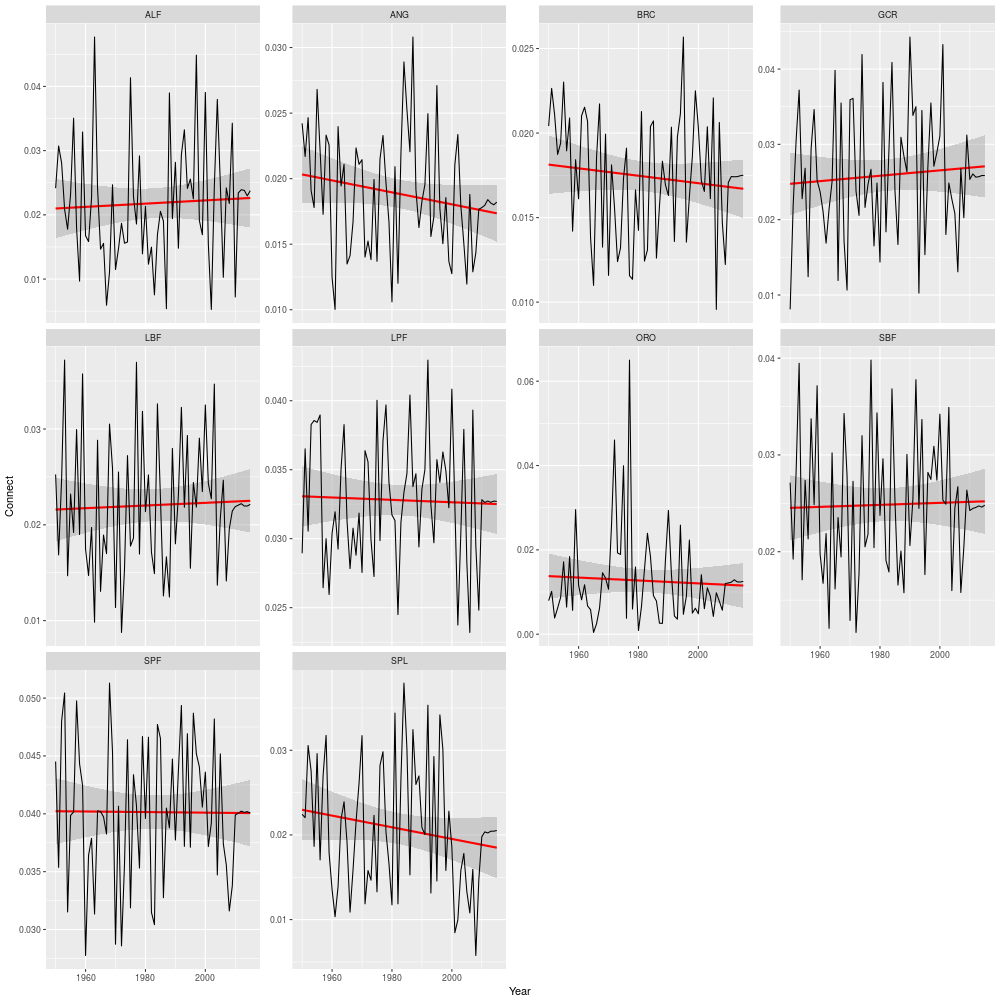
\includegraphics[width=.9\linewidth]{img/connectivity.png}
\caption{Average connectivity by year and FG}
\end{figure}
\end{itemize} % ends low level

\item Recruitment model
\label{sec-5-2-1-10-2}%
\begin{itemize}

\item Estimation of B-H parameter
\label{sec-5-2-1-10-2-1}%
\begin{itemize}
\item The Formula used is the option 3 for atlatnis
  R$_{c}$=(Sp * BHa)/Biomass + BHb
\item Sp = ((Wsp * FSP - KSPA ) - (Wsp - W)) * Nm * FSPB
\item Asumptions
\begin{itemize}
\item Wsp-W = 0; the indivifual are all at optimal reproductive stage (the same wieight)
\item Wsp =  weight * 1.4; the individual use in average 40\% of their weigth in reproduction
\item Nm and Biomass = The biomass calculated is based on the number of individual. I use the allometric relationship (calculated before)
\item The sorvival between one year an the other is based on the Natural mortality and the losses based on the connectivity
\begin{itemize}
\item Biomas$_{\mathrm{t+1}}$ = Biomas(t)*exp(-M) + Rec$_{t}$ * Survive
\end{itemize}
\item FSPB I assume that all of the individual are mature at that age.

\begin{verbatim}
## ~~~~~~~~~~~~~~~~~~~~~~~~~~~~~~~~~~~~~~~~~~~~~~~~~~~~~~~~~~~~~~~~~~~~~~ ##
## ~                  Beverton-holtz parameter estimation               ~ ##
## ~~~~~~~~~~~~~~~~~~~~~~~~~~~~~~~~~~~~~~~~~~~~~~~~~~~~~~~~~~~~~~~~~~~~~~ ##
library(ascii)
options(asciiType = "org")
source('/home/demiurgo/Documents/PhD/Atlantis_Model/tools/General_tools/Atlantis_tools.R')
##~ Read data
data <- read.csv('/home/demiurgo/Documents/PhD/Functional_groups/Spawning/B-H.csv')
##~ Weight at mat
data$w.at.m <- with(data,  weight2N(alometric(l.mat,alf.all,beta.all), metric = 'g'))
##~ Weight at spawning
data$wsp <- data$w.at.m * 1.4
##~ Calculating the amount of Spawn (Sp)
data$Sp  <- with(data, (wsp * FSP - KSPA) * Nm * prop)
data$bio <- with(data, wsp * Nm)

                                        #data$KSPA <- 1

b.h <- function(Sp, biomass, alfa, beta, lag, Surv, M){
    Ro    <- (Sp * exp(alfa)) / (biomass + exp(beta))
    B.lag <- (Ro * Surv) * exp( - M * lag) + biomass * exp( - M * lag)
    return(B.lag)
}


for( i in 1 :  dim(data)[1]){
    ## Estimation of parameters
    Bio     <- data$bio[i]
    Sp      <- data$Sp[i]
    biomass <- data$biomass[i]
    Age.mat <- data$Age.mat[i]
    Survive <- data$Survive[i]
    M       <- 0.2
    ## optim
    MRSS <- function(biom, par){
        (biom -  b.h(Sp, Bio, par[1], par[2], Age.mat, Survive, M)) ^ 2
    }
    ## trying diffetente starting values
    for( t in 1 : 100){
        res <- optim(par = c(log(t), log(t)) , MRSS, biom = Bio, method = 'CG' )
        if(t == 1) res.tmp <- res
        if(res$value < res.tmp$value){
            res.tmp <- res
        }
    }
    data$Alfa.bh[i] <- exp(res.tmp$par[1])
    data$Beta.bh[i] <- exp(res.tmp$par[2])
}

cap   <- 'Estimation of the Beverton-holt parameters'
b     <- ascii(data, header = T,  include.rownames = FALSE, include.colnames = T, caption = cap)
print(b)
\end{verbatim}
\end{itemize}

\begin{center}
\begin{tabular}{lrrrrrrrrrrrrrrr}
 FG   &   FSP  &      KSPA  &       Nm  &  alf.all  &  beta.all  &  Age.mat  &     l.mat  &  Survive  &  prop  &          w.at.m  &             wsp  &                Sp  &                bio  &              Alfa.bh  &  Beta.bh  \\
\hline
 ALF  &  0.31  &    939.02  &  1000.00  &     0.05  &      2.84  &     6.00  &     54.82  &     0.06  &  1.00  &        26221.61  &        36710.26  &       10441160.66  &        36710260.20  &        4761569555.28  &     5.00  \\
 ANG  &  0.29  &    137.78  &  1000.00  &     0.00  &      2.83  &     2.00  &    131.18  &     0.03  &  0.50  &        30160.64  &        42224.89  &        6053719.07  &        42224890.16  &        4501806169.25  &     6.00  \\
 BRC  &  0.31  &    364.60  &  1000.00  &     0.01  &      3.15  &     5.00  &     50.56  &     0.02  &  1.00  &        12267.89  &        17175.05  &        4959666.03  &        17175051.72  &        6017641254.46  &    93.99  \\
 GCR  &  0.29  &     56.18  &  1000.00  &     0.53  &      2.84  &     6.00  &     14.75  &     0.06  &  0.50  &         7068.33  &         9895.66  &        1406780.33  &         9895657.45  &        2878490550.20  &    71.99  \\
 LBF  &  0.32  &   4638.99  &  1000.00  &     0.00  &      3.88  &    12.00  &    101.51  &     0.11  &  0.20  &       101342.45  &       141879.43  &        8152485.34  &       141879427.16  &      233211625935.31  &    24.00  \\
 LPF  &  0.29  &    117.17  &  1000.00  &     0.03  &      2.73  &     3.00  &     70.83  &     0.08  &  0.25  &        20670.09  &        28938.12  &        2068721.35  &        28938122.08  &        4033992076.64  &     9.00  \\
 ORO  &  0.47  &   6915.95  &  1000.00  &     0.04  &      2.91  &    33.00  &     51.66  &     0.04  &  0.67  &        27180.73  &        38053.03  &        7349211.59  &        38053026.66  &     3579941264946.31  &    39.00  \\
 OTA  &  0.37  &  74926.06  &  1000.00  &     3.88  &      2.07  &     5.00  &  31597.16  &     0.80  &  0.33  &  52467703339.25  &  73454784674.95  &  8968804483211.89  &  73454784674952.41  &  1292141376737862.00  &    95.00  \\
 SBF  &  0.31  &    411.93  &  1000.00  &     7.08  &      1.37  &     3.00  &     60.96  &     0.08  &  1.00  &        12674.96  &        17744.94  &        5089000.57  &        17744937.33  &         629201273.76  &    29.00  \\
 SPF  &  0.32  &    331.33  &  1000.00  &     0.01  &      3.14  &     3.00  &     48.30  &     0.06  &  1.00  &         8952.58  &        12533.61  &        3679425.24  &        12533610.14  &         608039026.03  &     5.00  \\
 SPL  &  0.35  &    609.71  &  1000.00  &     0.96  &      2.72  &     6.00  &     12.94  &     0.03  &  0.50  &         6467.00  &         9053.79  &        1279558.82  &         9053793.27  &        4266434446.74  &    27.00  \\
\end{tabular}
\end{center}


\begin{itemize}
\item Estimation recruitment coral
\begin{itemize}
\item These species have low growth rate and low mortality Roger et al

\begin{verbatim}
library(ascii)
options(asciiType = "org")

## Initial values

c.a    <- 8
c.b    <- 7
c.c    <- 20
K      <- 10000 # minimum ammount of recruit
# number of posible colonies
init.B <- 10000000

coral <- function(K, c.a, c.b, c.c, biom){
    K + c.a * max(c(0, (c.b - exp(-c.c * biom))))
}
## hacer un arreglo en matrix para calcular la superficie de verosimilitud para los valores de los parametros

biomass <- vector('numeric',100)
biomass[1] <- init.B

for(i in 2 : 100){
    rec          <- coral(K, c.a, c.b, c.c, biomass[i-1])
    biomass[i]   <- biomass[i - 1] * exp(-0.15) + rec
}
\end{verbatim}
\end{itemize}

\end{itemize}
\end{itemize}


\item EStimation of weight at recruitment\\
\label{sec-5-2-1-10-2-2}%
\begin{verbatim}
library(ascii)
options(asciiType = "org")
source('/home/demiurgo/Documents/PhD/Atlantis_Model/tools/General_tools/Atlantis_tools.R')
##~ Read data
data <- read.csv('/home/demiurgo/Documents/PhD/Functional_groups/Spawning/weight_rec.csv')

data$weight <- with(data, ifelse(is.na(weight),
                                 alometric(size, Alpha, Beta),
                                 weight))
##~ estimation of structural and reserve wight for recruitment
data <- cbind(data, with(data, weights(FG, weight,'g'))[, 2 : 3])

cap <- 'Structural and reserve wight for recruitment'
b     <- ascii(data, header = T,  include.rownames = FALSE, include.colnames = T, caption = cap)
print(b)
\end{verbatim}

\begin{center}
\begin{tabular}{lrrrrlrr}
 FG   &   weight  &   size  &  Alpha  &  Beta  &  Reference       &  structural  &   reserve  \\
\hline
 ALF  &     0.15  &   1.50  &   0.05  &  2.84  &  Mundy1990       &        0.36  &      0.97  \\
 ANG  &     0.69  &   5.80  &   0.00  &  2.83  &  Miller2009      &        1.65  &      4.37  \\
 BRC  &     0.28  &   3.04  &   0.01  &  3.15  &  Bruce2001       &        0.67  &      1.77  \\
 GCR  &     9.61  &   2.77  &   0.53  &  2.84  &  Anger1983       &       23.09  &     61.18  \\
 LBF  &     0.16  &   5.30  &   0.00  &  3.90  &  Mujica          &        0.38  &      1.01  \\
 LPF  &     4.40  &         &   0.07  &  2.50  &  Lopez 2000      &       10.57  &     28.01  \\
 ORO  &     0.01  &   0.53  &   0.04  &  2.91  &  Zeldis          &        0.02  &      0.05  \\
 OTA  &  8600.00  &         &   3.88  &  2.07  &  Osman           &    20668.11  &  54770.49  \\
 SBF  &    11.07  &   3.00  &   1.58  &  1.77  &  Billy Database  &       26.61  &     70.53  \\
 SPF  &     0.06  &   2.00  &   0.01  &  3.14  &  Sawada          &        0.15  &      0.40  \\
 SPL  &     0.96  &   1.00  &   0.96  &  2.72  &  Porobic         &        2.31  &      6.13  \\
 VID  &  1586.96  &  58.02  &   0.01  &  3.11  &  Billy Database  &     3813.90  &  10106.83  \\
\end{tabular}
\end{center}


\end{itemize} % ends low level
\end{itemize} % ends low level
\paragraph*{LFD by cohorts}
\label{sec-5-2-1-11}
\begin{itemize}

\item Age groups non-Crustaceans\\
\label{sec-5-2-1-11-1}%
In this secction I use the data form the Database to get the number of organism by cohort. The cohorts used here matches the cohort on Atlantis

\begin{verbatim}
rm(list = ls())
library(ascii)
options(asciiType = "org")
library(ggplot2)
source('/home/demiurgo/Documents/PhD/Atlantis_Model/tools/General_tools/Atlantis_tools.R')
## data
lf    <- read.csv('/home/demiurgo/Documents/PhD/Functional_groups/cohorts/LF.csv')
p.l   <- read.csv('/home/demiurgo/Documents/PhD/Functional_groups/cohorts/params.csv', row.names=1)
##~ Grupos funcionales
lf    <- FG(lf, 2)
lf.fg <- split(lf, lf$FG)  # split by functional group
for(i in 1 : ncol(p.l)){
    ##~ Looking FG
    t.fg   <- which(names(lf.fg) %in% colnames(p.l)[i])
    len    <- lf.fg[[t.fg]][, 3]
    if(colnames(p.l)[i] %in% c('ANG', 'LBF', 'SBF')) len <- lf.fg[[t.fg]][, 4]
    intv   <- seq(from = p.l[5, i],  by = p.l[5, i], length = (p.l[4, i] / p.l[5, i]) - 1)
    temp.l <- vb(p.l[1, i], p.l[3, i], p.l[2, i], 1 : p.l[4, i])
    t.out  <- hist(len, breaks = c(0, temp.l[intv], max(len, na.rm = T)), plot = FALSE)
    ## reconstruction age aproximation using lineal regretion
    t.out  <- with(t.out, data.frame(Mid = mids, Count = counts))
    max.p  <- which.max(t.out[, 2])
    min.p  <- which.min(t.out[max.p : nrow(t.out), 2])
    reg.o  <- with(t.out, lm(Count ~ Mid, data = t.out[max.p : min.p, ]))
    ## Recalculating the data
    for( j in 1 : (max.p - 1)){
        t.out[j, 2] <- t.out[j, 1]  * reg.o$coef[2] + reg.o$coef[1]
    }
    ## Correction of Zeros
    t.out$Count <- ifelse(t.out$Count == 0, min(t.out$Count[t.out$Count > 0], na.rm = T), t.out$Count)
    t.out$Prop  <- t.out$Count / sum(t.out$Count, na.rm = T)
    age.c       <- c(paste('Cohort 0', 1 : 9, sep = ''),  'Cohort 10')
    t.out       <- cbind(FG = as.factor(colnames(p.l)[i]), Age_group = age.c[1 : nrow(t.out)], t.out)
    if(i == 1){
        output <- t.out
    } else {
        output <- rbind(output, t.out)
    }
}
## Table
cap     <- 'Proportion of Individual by Cohort,  based on the configuration of Atlantis'
tab.out <- xtabs(Prop ~ FG + Age_group, output)
png('img/Cohorts.png', height = 1000, width = 1000)
sp    <- ggplot(data = output, aes(Age_group, Prop, group = 1))+ geom_line()
sp + facet_wrap(~FG, ncol = 4, scales = 'free_y')
invisible(dev.off())
b     <- ascii(tab.out, header = T,  include.rownames = TRUE, include.colnames = TRUE, caption=cap, digits=3)
print(b)
\end{verbatim}

\begin{center}
\begin{tabular}{llrrrrrrrrrr}
              &       &  \textbf{Age_group}  &             &             &             &             &             &             &             &             &             \\
              &       &           Cohort 01  &  Cohort 02  &  Cohort 03  &  Cohort 04  &  Cohort 05  &  Cohort 06  &  Cohort 07  &  Cohort 08  &  Cohort 09  &  Cohort 10  \\
\hline
 \textbf{FG}  &  ANG  &               0.576  &      0.287  &      0.113  &      0.012  &      0.001  &      0.001  &      0.001  &      0.001  &      0.001  &      0.006  \\
              &  BRC  &               0.436  &      0.238  &      0.168  &      0.063  &      0.032  &      0.018  &      0.011  &      0.008  &      0.005  &      0.020  \\
              &  VID  &               0.867  &      0.092  &      0.037  &      0.005  &      0.000  &      0.000  &      0.000  &      0.000  &      0.000  &      0.000  \\
              &  LBF  &               0.551  &      0.244  &      0.137  &      0.019  &      0.008  &      0.004  &      0.004  &      0.004  &      0.004  &      0.027  \\
              &  SBF  &               0.473  &      0.269  &      0.144  &      0.057  &      0.028  &      0.004  &      0.004  &      0.004  &      0.004  &      0.013  \\
              &  LPF  &               0.512  &      0.402  &      0.051  &      0.010  &      0.007  &      0.010  &      0.005  &      0.002  &      0.000  &      0.001  \\
              &  SPF  &               0.201  &      0.185  &      0.177  &      0.171  &      0.166  &      0.077  &      0.015  &      0.002  &      0.002  &      0.005  \\
              &  ALF  &               0.384  &      0.235  &      0.152  &      0.144  &      0.063  &      0.016  &      0.002  &      0.002  &      0.002  &      0.002  \\
              &  ORO  &               0.432  &      0.252  &      0.149  &      0.084  &      0.046  &      0.018  &      0.006  &      0.004  &      0.004  &      0.004  \\
\end{tabular}
\end{center}



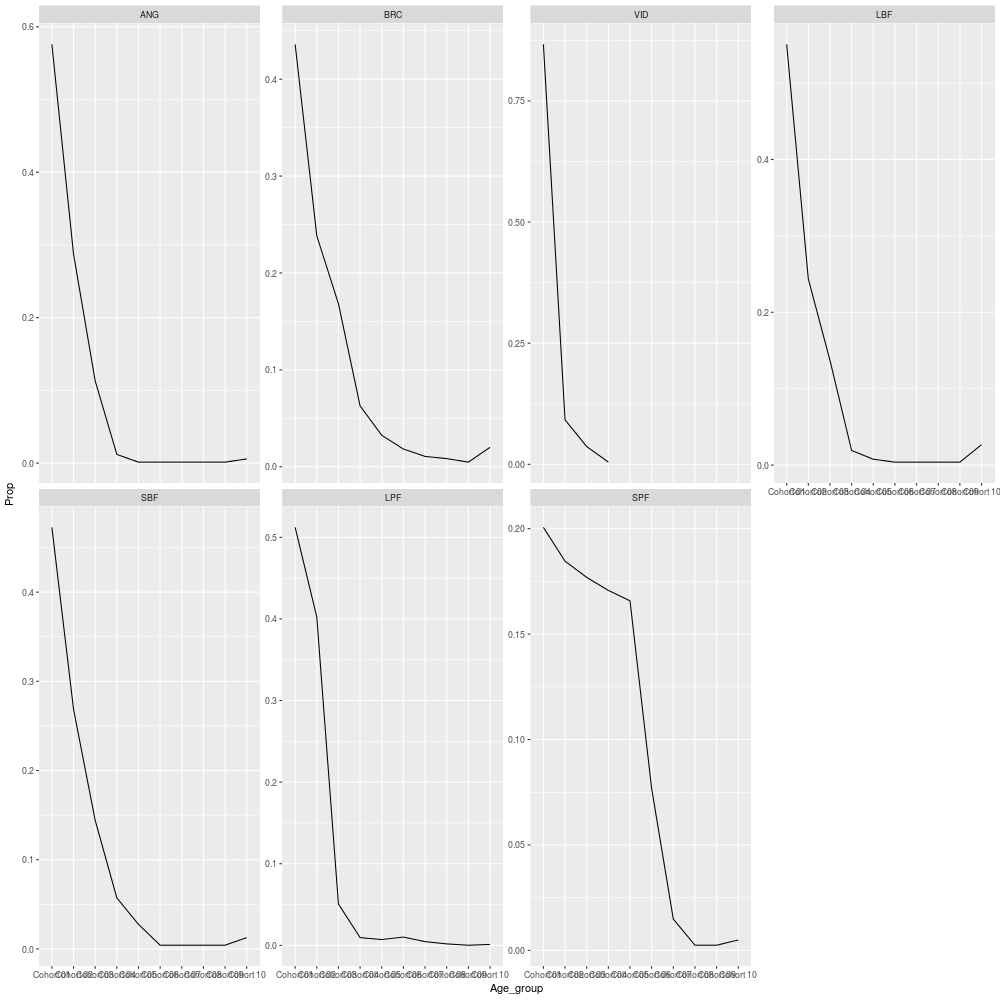
\includegraphics[width=.9\linewidth]{/home/demiurgo/Documents/PhD/Atlantis_Model/model_JFR/MandM/img/Cohorts.png}


\item Crustaceans SPL and GCR
\label{sec-5-2-1-11-2}%
\begin{itemize}
\item To calculate the size at age of each individual I used the following steps:
\begin{itemize}
\item Assume that the average maximum size (Linf) is 314mm (Manriquez,2016)
\item The minimum size at settlement is 10 mm (Porobic pers. comm.)
\item Use the transition matrix values
\end{itemize}
\end{itemize}

\begin{verbatim}
library(ascii)
options(asciiType = "org")
library(ggplot2)
source('/home/demiurgo/Documents/PhD/Atlantis_Model/tools/General_tools/Atlantis_tools.R')
k.g       <- 0.06985
beta.g    <- 1
Lo        <- 10
Linf1      <- 214
Linf2      <- 314
## Testing old linf from Arana
f.size    <- NULL
f.size[1] <- Lo
y         <- 1
while((Linf1-f.size[y]) > 1){
    y <- y + 1
    f.size[y] <- f.size[y-1] + mgrowth(Linf1, f.size[y-1], k.g)
    if((f.size[y] - f.size[y - 1]) > 1) y.delta <- y
}
f.size2    <- NULL
f.size2[1] <- Lo
y         <- 1
while((Linf2-f.size2[y]) > 1){
    y <- y + 1
    f.size2[y] <- f.size2[y-1] + mgrowth(Linf2, f.size2[y-1], k.g)
    if((f.size2[y] - f.size2[y - 1]) > 1) y.delta2 <- y
}
png('img/AgeClass_SPL.png', height = 1000, width = 1000)
par(mfcol = c(2, 1))
plot(f.size, xlab = 'Age [Years]', ylab = 'Length [mm]', pch = 20, col = 'red', bty = 'n', main = 'old Linf = 214')
y.delta   <- round(y.delta / 10, 0) * 10  ## the is the maximum number of age groups
abline(v = seq(from = 1, to = y.delta, by = 4), lty = 2) ## I will use the last age class as a group +
axis(3, at = seq(from = 2, to = y.delta , by = 4), label= paste0('AC-', 1 : 10), las=2)
fin.size  <- seq(from = 1, to = 37, by=4)
plot(f.size2, xlab = 'Age [Years]', ylab = 'Length [mm]', pch = 20, col = 'red', bty = 'n', main = 'New Linf = 314')
## because Atlantis is using round number I will round the maximum value of y.delta to the closest number
y.delta2   <- round(y.delta2 / 10, 0) * 10  ## the is the maximum number of age groups
abline(v = seq(from = 1, to = y.delta2, by = 4), lty = 2) ## I will use the last age class as a group +
axis(3, at = seq(from = 2, to = y.delta2, by = 4), label= paste0('AC-', 1 : 10), las=2)
fin.size2  <- seq(from = 1, to = 37, by=4)
invisible(dev.off())
out       <- data.frame(AgeClass = 1:10, minSize.old= f.size[fin.size], maxSize.old = f.size[fin.size + 4],
                        minSize.new= f.size2[fin.size2], maxSize.new = f.size2[fin.size2 + 4])
cap <- 'Age Classes and size at age for lobster'
b     <- ascii(out, header = T,  include.rownames = FALSE, include.colnames = TRUE, caption=cap, digits=3)
print(b)
\end{verbatim}

\begin{center}
\begin{tabular}{rrrrr}
 AgeClass  &  minSize.old  &  maxSize.old  &  minSize.new  &  maxSize.new  \\
\hline
    1.000  &       10.000  &       59.728  &       10.000  &       84.104  \\
    2.000  &       59.728  &       97.333  &       84.104  &      140.144  \\
    3.000  &       97.333  &      125.772  &      140.144  &      182.524  \\
    4.000  &      125.772  &      147.279  &      182.524  &      214.573  \\
    5.000  &      147.279  &      163.543  &      214.573  &      238.809  \\
    6.000  &      163.543  &      175.843  &      238.809  &      257.138  \\
    7.000  &      175.843  &      185.144  &      257.138  &      270.999  \\
    8.000  &      185.144  &      192.178  &      270.999  &      281.481  \\
    9.000  &      192.178  &      197.497  &      281.481  &      289.408  \\
   10.000  &      197.497  &      201.520  &      289.408  &      295.402  \\
\end{tabular}
\end{center}



\end{itemize} % ends low level
\paragraph*{Estimation of the mean Weight}
\label{sec-5-2-1-12}

\begin{itemize}
\item Based on the catch data and the data at age available I calculated the mean weight for several groups
\end{itemize}

\begin{verbatim}
## Estimation of the mean weight for the FG
rm(list=ls())
library(ascii)
options(asciiType = "org")
source('/home/demiurgo/Documents/PhD/Atlantis_Model/tools/General_tools/Atlantis_tools.R')
datos <- read.csv('/home/demiurgo/Documents/PhD/Functional_groups/length_weight/length_weight_jf.csv')
w.fg  <- FG(datos, 2)
w.fg  <- split(w.fg, w.fg$FG)
## estimation of mean weight
weigth <- vector('numeric')
for( i in 1: length(w.fg)){
weigth[i] <- mean(w.fg[[i]]$weight)
}
## output
cap <- 'Mean weight for Functional Group (FG)'
out <- data.frame(FG = names(w.fg), Mean.Weight = weigth)
b   <- ascii(out, header = T,  include.rownames = FALSE, include.colnames = TRUE, caption=cap)
print(b)
\end{verbatim}
\begin{table}[htb]
\caption{Mean weight for Functional Group (FG)}
\begin{center}
\begin{tabular}{lr}
 FG   &  Mean.Weight  \\
\hline
 ANG  &      1013.75  \\
 BRC  &       745.93  \\
 CHO  &      4298.08  \\
 GCR  &       697.06  \\
 LBF  &      4125.24  \\
 LPF  &       484.88  \\
 OCT  &       640.00  \\
 OTA  &     75857.01  \\
 SBF  &      1203.85  \\
 SPF  &       318.45  \\
 SPL  &       630.62  \\
 VID  &      3755.67  \\
\end{tabular}
\end{center}
\end{table}
\paragraph*{Temperature}
\label{sec-5-2-1-13}
\begin{itemize}

\item Recruitment\\
\label{sec-5-2-1-13-1}%
\begin{center}
\begin{tabular}{lrrll}
 FG   &   Max  &  Min  &  Reference                    &  Specie           \\
\hline
 SPL  &    25  &    8  &  Whale and Fogarty 2007       &  lobsters         \\
      &        &    5  &  Waddy and aiken 1995         &  H. americanus    \\
      &        &  9.8  &                               &  J. edwarsii      \\
 GCR  &    32  &    2  &  Prentice and Schneider 1978  &  Dungeness crab   \\
      &    19  &    4  &  Hardy and Dutil 1994         &  Snow crab        \\
      &        &   10  &  hill 1974                    &  Portunid crab    \\
      &  28.5  &   10  &  Maestre et al 2015           &  Chaceon affinis  \\
\end{tabular}
\end{center}



\item Optimal temperature\\
\label{sec-5-2-1-13-2}%
\begin{center}
\begin{tabular}{lrrlll}
 FG   &    Opt. temp  &  Value Used  &  Reference                   &  Species                     &  Observations                              \\
\hline
 SPL  &           17  &          17  &  Dupre1985                   &  Jasus frontalis             &                                            \\
      &        16-18  &              &  Dubber 2004                 &  Jasus lalandii              &                                            \\
\hline
 GCR  &            5  &           5  &  Ahumada 2009                &  Chaceon chislensis          &                                            \\
\hline
 BRC  &        16-18  &          17  &  Neuheimer 2011              &  Cheilodactylus spectabilis  &                                            \\
\hline
 ORO  &          4-5  &           5  &  Dunn 2011                   &  Orange Roughy               &                                            \\
\hline
 ANG  &           17  &          17  &  EOL                         &  eels moray                  &                                            \\
\hline
 ALF  &        16-19  &          17  &  Lehedoy 1995                &  Alfonsino                   &                                            \\
\hline
 CHO  &         8-17  &          13  &  Fishbase                    &  Squalus mitsukurii          &                                            \\
\hline
 OCT  &        16-21  &        18.5  &  Delgado 2011                &  Octopus vulgaris            &                                            \\
\hline
 SQD  &        15-28  &          10  &  Nigmatullin 2001            &  Dosidicus gigas             &                                            \\
      &         3-10  &              &  Watanabe 2006               &  Squids (vampirotheutis)     &                                            \\
\hline
 COR  &         4-13  &           9  &  Guinote 2005                &  Deep sea corals             &                                            \\
      &         4-15  &              &  Brooke 2013                 &  Lophelia pertusa            &                                            \\
\hline
 LPF  &           20  &          20  &  Fishbase                    &  Pseudocaranx dented         &                                            \\
\hline
 SPF  &        23-29  &              &  Encyclopedia of Life (EOL)  &  Kyphosus cinerascens        &                                            \\
      &           27  &       20.75  &  Fishbase                    &  Kyphosus cinerascens        &                                            \\
      &  16.92-17.02  &              &  EOL                         &  Scartichthys variolatus     &                                            \\
      &  14.66-17.65  &              &                              &  Callanthias allporti        &                                            \\
\hline
 SBF  &        17.07  &              &  EOL                         &  Chironemus bicornis         &                                            \\
      &        13.27  &      13.025  &  EOL                         &  Plectranthias exsul         &                                            \\
      &   8.41-13.35  &              &  EOL                         &  Helicolenus lengerichi      &                                            \\
\hline
 LBF  &   5.44-25.74  &              &  EOL                         &  Polyprion oxygeneios        &  The range is too high so I didn't use it  \\
      &        15-21  &       17.48  &  Khan 2015                   &  Polyprion oxygeneios        &                                            \\
      &  16.92-17.02  &              &  EOL                         &  Lotella fernandeziana       &                                            \\
\hline
 SCR  &   8.46-13.87  &      12.218  &  EOL                         &  Paromola cuvieri            &                                            \\
      &   8.85-17.69  &              &  EOL                         &  Ovalipes trimaculatus       &                                            \\
\hline
 BCA  &        14.04  &              &  EOL                         &  Phymactis clematis          &                                            \\
      &   8.32-20.98  &       17.37  &  EOL                         &  Corynactis                  &                                            \\
      &    15.7-21.3  &              &  Delorme 2013                &  Evechinus chloroticus       &                                            \\
      &        23.88  &              &  EOL                         &  Centrostephanus asteriscus  &                                            \\
\hline
 MOL  &        14-20  &      19.752  &  Rabi and Maravi 1997        &  Concholepas concholepas     &                                            \\
      &  20.69-24.32  &              &  EOL                         &  Thacacera                   &                                            \\
\end{tabular}
\end{center}



\begin{itemize}

\item Temperature tolerance (Griffin model)
\label{sec-5-2-1-13-2-1}%
\end{itemize} % ends low level
\end{itemize} % ends low level
\paragraph*{Oxigen}
\label{sec-5-2-1-14}
\begin{itemize}

\item Oxygen model used for epibenthic invertebrate \textbf{Quadratic limitation} (O2case = 3)
\label{sec-5-2-1-14-1}%
\begin{itemize}
\item Calculates both ambient and depth based limitation and uses the larger of the two values as the oxygen scalar dO2
\item \textbf{Ambient oxygen limitation}: uses ambient oxygen levels O amb , lethal oxygen concentration (KO2\_XXX, mgO2m-3) and limiting oxygen concentration (KO2lim\_XXX, mgO2 m -3 ) parameters. Remember that oxygen solubility in seawater at 5C and 1bar pressure is 10 mg/l or 10000 mg m -3 .

\begin{center}
\begin{tabular}{lrrl}
 FG   &  KO2 (mg / m3)  &  KO2lim  &  reference     \\
\hline
 SPL  &           1320  &    2900  &  Mcleese 1956  \\
 GCR  &           2450  &    3210  &  Vaquer2008    \\
 SCR  &           2450  &    3210  &                \\
 BFF  &            890  &     690  &                \\
 LPH  &              0  &          &                \\
 SPH  &              0  &          &                \\
 SUR  &            890  &    1220  &                \\
 MOL  &            890  &    1990  &                \\
 PB   &              0  &          &                \\
 BB   &              0  &          &                \\
\end{tabular}
\end{center}


\end{itemize}




\begin{verbatim}
## ~~~~~~~~~~~~~~~~~~~~~~~~~~~~~~~~~~~~~~~~~~~~~~~~~~~~~~~~~~~~~~~~~~~~~~~~~~~~~~~~ ##
## ~                     Oxigen mortality and tolerance functions                 ~ ##
## ~~~~~~~~~~~~~~~~~~~~~~~~~~~~~~~~~~~~~~~~~~~~~~~~~~~~~~~~~~~~~~~~~~~~~~~~~~~~~~~~ ##

##
## Oxigen functions
##~~~~~~~~~~~~~~~~~~~~

lim_oxi <- function(Oxi, KO2, KO2lim){
    KO2 = 1320
    KO2lim = 2900
    Oxi = 1:8000
    oxi2 <- ifelse(Oxi >= KO2 & KO2lim >= KO2, ((Oxi - KO2)^2 / ((Oxi - KO2)^2 + (KO2lim - KO2) ^ 2)),
        ifelse(Oxi >= KO2 & KO2lim < KO2, 1, 0))
        return(oxi2)
    }
\end{verbatim}

\end{itemize} % ends low level
\paragraph*{Extra Mortality}
\label{sec-5-2-1-15}

     I'm not including xxplicit fish mortality by season (mS$_{\mathrm{FDXXX}}$) and seabird and mamal induced mortality (mS$_{\mathrm{SBXXX}}$)
\paragraph*{Bibliography that I need}
\label{sec-5-2-1-16}

\begin{itemize}
\item $\Box$ Sepulveda y Pequeño,  Fauna ictica del archipielago de Juan Fernandez. En P. Arana (ed). Investigaciones Marinas en el Archipiélago de Juan Fernández. Esc. Ciencias del Mar, UCV, Valparaíso
\item $\Box$ Meléndez, C.R. y C. Villalba. 1992. Nuevos registros y antecedentes para la ictiofauna del archipiélago de Juan Fernández, Chile. Estud. Oceanol. 11 : 3 - 29
\item $\Box$ TORRES D (1987) Antecedentes sobre el lobo fino de Juan Fernández Arctocephalus philippii y proyecciones para su estudio. In: Castilla JC (ed) Islas oceánicas chilenas: conocimiento científico y necesidades de investigaciones: 287-317. Ediciones Universidad Católica de Chile, Santiago, Chile.
\end{itemize}
\paragraph*{Codes}
\label{sec-5-2-1-17}


\begin{center}
\begin{tabular}{lllll}
 Code  &  Functional Groups     &     &  Simil SETas  &  Other  \\
\hline
 SPL   &  Spiny lobster         &     &               &         \\
 GCR   &  Golden Crab           &     &  BMD          &         \\
 BRC   &  Breca                 &     &  FDS          &  FDM    \\
 VID   &  Vidriola              &     &  FVT          &  FVO    \\
 ORO   &  Orange Roughy         &     &  FDF          &  FDD    \\
 ALF   &  Alfonsino             &     &  FDD          &  FDM    \\
 ANG   &  Anguila               &     &  FVD          &  FVD    \\
 CHO   &  Chondrichtyans        &     &  SHB          &         \\
 OTA   &  Otariid               &     &  PIN          &         \\
 CET   &  Cetaceans             &     &  WHS          &  WHB    \\
 BIR   &  Birds                 &     &  SB           &         \\
 OCT   &  Octupus               &     &  CEP          &         \\
 SUR   &  Sea urchins           &     &  BFS          &  BFF    \\
 MOL   &  Mollusca              &     &  BFS          &  BFF    \\
 SCR   &  Small crustaceans     &     &  BMD          &         \\
 LPF   &  Large pelagic fish    &     &  FVS          &  FDE    \\
 SPF   &  Small pelagic fish    &     &  FVS          &         \\
 SBF   &  Small benthic fish    &     &  FDS          &  FDD    \\
 LBF   &  Large benthic fish    &     &  FVD          &  FDD    \\
 SZO   &  Small Zooplankton     &     &               &         \\
 MZO   &  Medium Zooplankton    &     &               &         \\
 LZO   &  Large Zooplankton     &     &               &         \\
 BFF   &  Deposit feeders       &     &               &         \\
 LPH   &  Large phytoplankton   &     &               &         \\
 SPH   &  Small phytoplankton   &     &               &         \\
 NO    &  Nitrate               &     &               &         \\
 MA    &  Macroalgae            &     &               &         \\
 PB    &  Pelagic Bacteria      &     &               &         \\
 BB    &  Sediment Bacteria     &     &               &         \\
 DL    &  Labile detritus       &     &               &         \\
 DR    &  Refractory detritrus  &     &               &         \\
 DC    &  Carrion               &     &               &         \\
\hline
\end{tabular}
\end{center}
\paragraph*{What is needed}
\label{sec-5-2-1-18}
\begin{itemize}

\item Look for the larval duration of other species
\label{sec-5-2-1-18-1}%

\item Poner el numero de individuos desovando
\label{sec-5-2-1-18-2}%
\end{itemize} % ends low level
\paragraph*{Resume of the configuration file}
\label{sec-5-2-1-19}


\begin{center}
\begin{tabular}{lllllllllllllllllllllllllllll}
\hline
 Recruitment         &       &       &  X    &  X    &  X    &  X    &  X    &  X    &  X    &       &  X    &  X    &  X    &  X    &       &       &       &       &       &       &       &      &      &       &       &      &      &      \\
 Ext reproduction    &  X    &  X    &  X    &  X    &  X    &  X    &  X    &  X    &  X    &  X    &  X    &  X    &  X    &  X    &       &       &       &       &       &       &       &      &      &       &       &      &      &      \\
 Vertebrate rep      &       &       &  X    &  X    &  X    &  X    &  X    &  X    &  X    &       &  X    &  X    &  X    &  X    &       &       &       &       &       &       &       &      &      &       &       &      &      &      \\
 IsPlanktivore       &       &       &  X    &  X    &  X    &  X    &  X    &  X    &       &       &  X    &  X    &  X    &  X    &       &       &       &       &       &       &       &      &      &       &       &      &      &      \\
 Local recruit       &  X    &  X    &  X    &  X    &  X    &  X    &  X    &  X    &       &  X    &  X    &  X    &  X    &  X    &       &       &  X    &       &       &  X    &  X    &      &      &       &       &      &      &      \\
 bears live young    &  X    &  X    &  X    &  X    &  X    &  X    &  X    &  X    &       &  X    &  X    &  X    &  X    &  X    &       &       &  X    &       &       &  X    &  X    &      &      &       &       &      &      &      \\
 Parental care       &  X    &  X    &  X    &  X    &  X    &  X    &  X    &  X    &       &  X    &  X    &  X    &  X    &  X    &       &       &  X    &       &       &  X    &  X    &      &      &       &       &      &      &      \\
 Feed while spawn    &  X    &  X    &  X    &  X    &  X    &  X    &  X    &  X    &       &  X    &  X    &  X    &  X    &  X    &       &       &  X    &       &       &  X    &  X    &      &      &       &       &      &      &      \\
 Temp feed eff       &  X    &  X    &  X    &  X    &  X    &  X    &  X    &  X    &       &  X    &  X    &  X    &  X    &  X    &       &       &  X    &       &       &  X    &  X    &      &      &       &       &      &      &      \\
 Temp sens           &  X    &  X    &  X    &  X    &  X    &  X    &  X    &  X    &       &  X    &  X    &  X    &  X    &  X    &       &       &  X    &       &       &  X    &  X    &      &      &       &       &      &      &      \\
 Hab depend]         &  X    &  X    &  X    &  X    &  X    &  X    &  X    &  X    &       &  X    &  X    &  X    &  X    &  X    &       &       &  X    &       &       &  X    &  X    &      &      &       &       &      &      &      \\
 D_depend            &  X    &  X    &  X    &  X    &  X    &  X    &  X    &  X    &       &  X    &  X    &  X    &  X    &  X    &       &       &  X    &       &       &  X    &  X    &      &      &       &       &      &      &      \\
 seeks Channel       &  X    &  X    &  X    &  X    &  X    &  X    &  X    &  X    &       &  X    &  X    &  X    &  X    &  X    &       &       &  X    &       &       &  X    &  X    &      &      &       &       &      &      &      \\
 Migrate out         &  X    &  X    &  X    &  X    &  X    &  X    &  X    &  X    &  X    &  X    &  X    &  X    &  X    &  X    &       &       &  X    &       &       &  X    &  X    &      &      &       &       &      &      &      \\
 Pred_func           &  X    &  X    &  X    &  X    &  X    &  X    &  X    &  X    &  X    &  X    &  X    &  X    &  X    &  X    &  X    &  X    &  X    &  X    &       &  X    &  X    &      &      &       &       &      &      &      \\
 Bioturvation        &       &       &       &       &       &       &       &       &       &       &       &       &       &       &       &       &       &  X    &       &       &  X    &      &      &       &       &      &      &      \\
 Bioirrigation       &       &       &       &       &       &       &       &       &       &       &       &       &       &       &       &       &  X    &  X    &       &       &  X    &      &      &       &       &      &      &      \\
 G. Griff Temp       &  X    &  X    &  X    &  X    &  X    &  X    &  X    &  X    &  X    &  X    &  X    &  X    &  X    &  X    &  X    &  X    &  X    &  X    &  X    &  X    &  X    &  X   &  X   &  X    &  X    &      &      &      \\
 Q10                 &  X    &  X    &  X    &  X    &  X    &  X    &  X    &  X    &  X    &  X    &  X    &  X    &  X    &  X    &  X    &  X    &  X    &  X    &  X    &  X    &  X    &  X   &  X   &  X    &  X    &      &      &      \\
 Calc Q10            &  X    &  X    &  X    &  X    &  X    &  X    &  X    &  X    &  X    &  X    &  X    &  X    &  X    &  X    &  X    &  X    &  X    &  X    &  X    &  X    &  X    &  X   &  X   &  X    &  X    &      &      &      \\
 Opt. Temp           &  X    &  X    &  X    &  X    &  X    &  X    &  X    &  X    &  X    &  X    &  X    &  X    &  X    &  X    &  X    &  X    &  X    &  X    &  X    &  X    &  X    &  X   &  X   &  X    &  X    &      &      &      \\
 Q10 Corr            &  X    &  X    &  X    &  X    &  X    &  X    &  X    &  X    &  X    &  X    &  X    &  X    &  X    &  X    &  X    &  X    &  X    &  X    &  X    &  X    &  X    &  X   &  X   &  X    &  X    &      &      &      \\
 ph sensitive        &  X    &  X    &  X    &  X    &  X    &  X    &  X    &  X    &  X    &  X    &  X    &  X    &  X    &  X    &  X    &  X    &  X    &  X    &  X    &  X    &  X    &  X   &  X   &  X    &  X    &      &      &      \\
 ph fecund           &  X    &  X    &  X    &  X    &  X    &  X    &  X    &  X    &  X    &  X    &  X    &  X    &  X    &  X    &  X    &  X    &  X    &  X    &  X    &  X    &  X    &  X   &  X   &  X    &  X    &      &      &      \\
 Nutri sens          &  X    &  X    &  X    &  X    &  X    &  X    &  X    &  X    &  X    &  X    &  X    &  X    &  X    &  X    &  X    &  X    &  X    &  X    &  X    &  X    &  X    &  X   &  X   &  X    &  X    &      &      &      \\
 pred availa         &  X    &  X    &  X    &  X    &  X    &  X    &  X    &  X    &  X    &  X    &  X    &  X    &  X    &  X    &  X    &  X    &  X    &  X    &  X    &  X    &  X    &  X   &  X   &  X    &  X    &      &      &      \\
 contract_tol        &  X    &  X    &  X    &  X    &  X    &  X    &  X    &  X    &  X    &  X    &  X    &  X    &  X    &  X    &  X    &  X    &  X    &  X    &  X    &  X    &  X    &  X   &  X   &  X    &  X    &      &      &      \\
 ph model            &  X    &  X    &  X    &  X    &  X    &  X    &  X    &  X    &  X    &  X    &  X    &  X    &  X    &  X    &  X    &  X    &  X    &  X    &  X    &  X    &  X    &  X   &  X   &  X    &  X    &      &      &      \\
 Inflection ph       &  X    &  X    &  X    &  X    &  X    &  X    &  X    &  X    &  X    &  X    &  X    &  X    &  X    &  X    &  X    &  X    &  X    &  X    &  X    &  X    &  X    &  X   &  X   &  X    &  X    &      &      &      \\
 optimal ph          &  X    &  X    &  X    &  X    &  X    &  X    &  X    &  X    &  X    &  X    &  X    &  X    &  X    &  X    &  X    &  X    &  X    &  X    &  X    &  X    &  X    &  X   &  X   &  X    &  X    &      &      &      \\
 ph correction       &  X    &  X    &  X    &  X    &  X    &  X    &  X    &  X    &  X    &  X    &  X    &  X    &  X    &  X    &  X    &  X    &  X    &  X    &  X    &  X    &  X    &  X   &  X   &  X    &  X    &      &      &      \\
 ph constant A       &  X    &  X    &  X    &  X    &  X    &  X    &  X    &  X    &  X    &  X    &  X    &  X    &  X    &  X    &  X    &  X    &  X    &  X    &  X    &  X    &  X    &  X   &  X   &  X    &  X    &      &      &      \\
 ph constant B       &  X    &  X    &  X    &  X    &  X    &  X    &  X    &  X    &  X    &  X    &  X    &  X    &  X    &  X    &  X    &  X    &  X    &  X    &  X    &  X    &  X    &  X   &  X   &  X    &  X    &      &      &      \\
 correction ph sca   &  X    &  X    &  X    &  X    &  X    &  X    &  X    &  X    &  X    &  X    &  X    &  X    &  X    &  X    &  X    &  X    &  X    &  X    &  X    &  X    &  X    &  X   &  X   &  X    &  X    &      &      &      \\
 Salinty sensivity   &  X    &  X    &  X    &  X    &  X    &  X    &  X    &  X    &  X    &  X    &  X    &  X    &  X    &  X    &  X    &  X    &  X    &  X    &  X    &  X    &  X    &  X   &  X   &  X    &  X    &      &      &      \\
 Correction Sainity  &  X    &  X    &  X    &  X    &  X    &  X    &  X    &  X    &  X    &  X    &  X    &  X    &  X    &  X    &  X    &  X    &  X    &  X    &  X    &  X    &  X    &  X   &  X   &  X    &  X    &      &      &      \\
 PP growth           &       &       &       &       &       &       &       &       &       &       &       &       &       &       &       &       &       &       &  X    &       &       &      &  X   &       &       &      &      &      \\
 PP light            &       &       &       &       &       &       &       &       &       &       &       &       &       &       &       &       &       &       &  X    &       &       &      &  X   &       &       &      &      &      \\
 PP nutrients        &       &       &       &       &       &       &       &       &       &       &       &       &       &       &       &       &       &       &  X    &       &       &      &  X   &       &       &      &      &      \\
 Bac nut req         &       &       &       &       &       &       &       &       &       &       &       &       &       &       &       &       &       &       &       &       &       &      &      &  X    &  X    &      &      &      \\
 Bac param pop       &       &       &       &       &       &       &       &       &       &       &       &       &       &       &       &       &       &       &       &       &       &      &      &       &       &      &      &      \\
 Space rectric       &       &       &       &       &       &       &       &       &       &       &       &       &       &       &       &       &       &       &  X    &       &       &      &      &       &       &      &      &      \\
 maxbiomass          &       &       &       &       &       &       &       &       &       &       &       &       &       &       &       &       &  X    &  X    &       &       &  X    &      &      &       &       &      &      &      \\
 Habitat dep         &  X    &  X    &  X    &  X    &  X    &  X    &  X    &  X    &  X    &  X    &  X    &  X    &  X    &  X    &  X    &  X    &  X    &  X    &  X    &  X    &  X    &  X   &  X   &  X    &  X    &      &      &      \\
 Juvenil and adult   &  X    &  X    &  X    &  X    &  X    &       &       &       &       &       &       &       &       &       &       &       &       &       &       &       &       &      &      &       &       &      &      &      \\
 refuge ad-juv       &  X    &  X    &  X    &  X    &  X    &       &       &       &       &       &       &       &       &       &       &       &       &       &       &       &       &      &      &       &       &      &      &      \\
 Max and min deph    &  X    &  X    &  X    &  X    &  X    &  X    &  X    &  X    &  X    &  X    &  X    &  X    &  X    &  X    &  X    &  X    &  X    &  X    &  X    &  X    &  X    &  X   &  X   &  X    &  X    &  X   &  X   &  X   \\
 Home range radius   &  X    &  X    &  X    &  X    &  X    &  X    &  X    &  X    &  X    &  X    &  X    &  X    &  X    &  X    &  X    &  X    &  X    &  X    &  X    &  X    &  X    &  X   &  X   &  X    &  X    &  X   &  X   &  X   \\
 Overlap             &  X    &  X    &  X    &  X    &  X    &  X    &  X    &  X    &  X    &  X    &  X    &  X    &  X    &  X    &  X    &  X    &  X    &  X    &  X    &  X    &  X    &  X   &  X   &  X    &  X    &  X   &  X   &  X   \\
 Function            &  SPL  &  GCR  &  BRC  &  ORO  &  ALF  &  CHO  &  OTA  &  CET  &  BIR  &  OCT  &  LPF  &  SPF  &  SBF  &  LBF  &  EUP  &  COP  &  SCR  &  BFF  &  PHY  &  SUR  &  MOL  &  NO  &  MA  &  BAC  &  BAS  &  DL  &  DR  &  DC  \\
 Spatial dist.       &  X    &  X    &  X    &  X    &  X    &  X    &  X    &  X    &  X    &  X    &  X    &  X    &  X    &  X    &       &       &       &       &       &  X    &  X    &      &      &       &       &      &      &      \\
 Vert. dist. inv.    &  X    &  X    &       &       &       &       &       &       &       &  X    &       &       &       &       &  X    &  X    &  X    &       &       &  X    &  X    &      &      &       &       &      &      &      \\
 Vert. dist. ver.    &       &       &  X    &  X    &  X    &  X    &  X    &  X    &       &       &       &       &       &       &       &       &       &       &       &       &       &      &      &       &       &      &      &      \\
\end{tabular}
\end{center}
\paragraph*{Mortality}
\label{sec-5-2-1-20}


\begin{center}
\begin{tabular}{lrl}
 FG   &  LM (F_\{initial\})  &  Reference     \\
\hline
 SPL  &            0.002507  &  MPA model     \\
 GCR  &        0.0009589041  &  Canales2009   \\
 BRC  &            0.000002  &  Arancibia     \\
 ORO  &        4.986301e-05  &  Wiff2016      \\
 ALF  &        0.0003383014  &  Wiff2016      \\
 SPF  &            0.000001  &  Guestimation  \\
 LPF  &            0.000001  &  Guestimation  \\
 SBF  &           0.0000002  &  Guestimation  \\
 LBF  &           0.0000001  &  Guestimation  \\
 VID  &         0.002739726  &  Using CCL     \\
\end{tabular}
\end{center}
\subsubsection*{Harvest file}
\label{sec-5-2-2}
\paragraph*{General setting}
\label{sec-5-2-2-1}


\begin{center}
\begin{tabular}{llrlrlrr}
 FG   &  fishery    &  Start (year)  &  End           &  Effort model  &  Selectivity  &  Change q  &  Change Eff  \\
\hline
 SPL  &  Trap       &             0  &                &             3  &  Logistic     &         1  &  1 (Chigre)  \\
 GCR  &  Trap       &  18263 (2000)  &                &             3  &  Logistic     &         0  &           0  \\
 ANG  &  Trap       &             0  &                &             3  &  Constant     &         0  &           0  \\
 SPF  &  Bait       &             0  &                &             3  &  Normal       &         0  &           0  \\
 LPF  &  Bait       &             0  &                &             3  &  Logistic     &         0  &           0  \\
 BRC  &  Bait       &             0  &                &             3  &  Logistic     &         0  &           0  \\
 LBF  &  Bait       &             0  &                &             3  &  Logistic     &         0  &           0  \\
 SBF  &  Bait       &             0  &                &             3  &  Logistic     &         0  &           0  \\
 BRC  &  Long line  &             0  &                &             3  &  Logistic     &         0  &           0  \\
 VID  &  Long line  &             0  &                &             3  &  Logistic     &         0  &           0  \\
 ORO  &  Trawl      &   17533(1998)  &  20454 (2006)  &             3  &  Logistic     &         0  &           0  \\
 ALF  &  Trawl      &   17533(1998)  &  22646 (2012)  &             3  &  Logistic     &         0  &           0  \\
 OCT  &  Pot        &             0  &                &             1  &  Logistic     &         0  &           0  \\
\end{tabular}
\end{center}
\paragraph*{TAC}
\label{sec-5-2-2-2}
\begin{itemize}

\item ALF
\label{sec-5-2-2-2-1}%
\begin{itemize}
\item start 2003 - jun - 01 (22446) (wiff 2016)
\begin{itemize}
\item catch 4752 tonns
\end{itemize}
\end{itemize}

\item ORO
\label{sec-5-2-2-2-2}%
\begin{itemize}
\item start 1999 (17897) Paya (2013)
\end{itemize}
\end{itemize} % ends low level
\paragraph*{Selectivity}
\label{sec-5-2-2-3}

\begin{itemize}
\item I used the values length of the catch to estimate the parameter for the selectivity curve
\end{itemize}

\begin{verbatim}
library(ascii)
options(asciiType = "org")
##-----------------------------------------#
##  obtener los limites de las capturas    #
##-----------------------------------------#
rm(list = ls())
source('/home/demiurgo/Documents/PhD/Atlantis_Model/tools/General_tools/Atlantis_tools.R')
## data
lf    <- read.csv('/home/demiurgo/Documents/PhD/Harvest/Selectivity/LF.csv')
## Grupos funcionales
lf    <- FG(lf, 2)
lf.fg <- split(lf, lf$FG)  # split by functional group
lf.fg <- lf.fg[ -c(2, 4, 7)] ## removed CHO OCT and ANG
png('img/Selectivity.png', height=900, width=900)
par(mfrow = c(3, 3), oma = c(3, 3, 1, 1), mar = c(1, 2, 3, 1))
out  <- NULL
for(i in 1 :  length(lf.fg)){
    ## checking the lenght of the vector
    if(sum(!is.na(lf.fg[[i]]$Fork_length)) > sum(!is.na(lf.fg[[i]]$Total_length))){
        col <- 3
    } else{
        col <- 4
    }
    lf.fg[[i]][, col] <- lf.fg[[i]][, col] /10
    ## range for the lengths
    rang    <- range(lf.fg[[i]][, col], na.rm = TRUE)
    h       <- hist(lf.fg[[i]][, col], breaks = seq(from = floor(rang[1]), to = ceiling(rang[2]), length = 10), plot = F)
    sel.obs <- data.frame(size = h$mids, prop = cumsum(h$counts) / sum(h$counts))
    ## estimations (using nls)
    size    <- sel.obs$size
    prop    <- sel.obs$prop
    sel.est <- nls(prop ~ selec(len = size, selb, lsm),
                   start = c(selb = 0.02, lsm = mean(sel.obs$size)))
    ## Generating the table with the parameters
    out <- rbind(out, data.frame(FG   = unique(lf.fg[[i]]$FG),
                                 Selb = coef(sel.est)[1], Lsm =  coef(sel.est)[2]))
    ## Ploting
    val.st <- fitted(sel.est)
    plot(sel.obs, pch = 19, main = unique(lf.fg[[i]]$FG), bty = 'n', xlab = '', ylab = '', las = 1)
    lines(size, val.st, col = 2, lty = 2, lwd = 2)
    if(i == 4) mtext('Selectivity', side = 2, line = 2.5)
    if(i == 8) mtext('Length (cm)', side = 1, line = 2.5)
}
dev.off()
## table with parameters
cap                  <- 'Selectivity parameters'
b                    <- ascii(out, header=T,  include.rownames = FALSE, include.colnames = TRUE, caption = cap, digit = 3)
print(b)
\end{verbatim}
\begin{table}[htb]
\caption{Selectivity parameters}
\begin{center}
\begin{tabular}{lrr}
 FG   &   Selb  &     Lsm  \\
\hline
 ALF  &  0.239  &  30.505  \\
 BRC  &  0.211  &  37.649  \\
 LBF  &  0.095  &  53.677  \\
 LPF  &  0.217  &  27.202  \\
 ORO  &  0.427  &  42.323  \\
 SBF  &  0.182  &  37.818  \\
 SPF  &  0.413  &  28.327  \\
 VID  &  0.159  &  64.993  \\
\end{tabular}
\end{center}
\end{table}


\begin{figure}[htb]
\centering
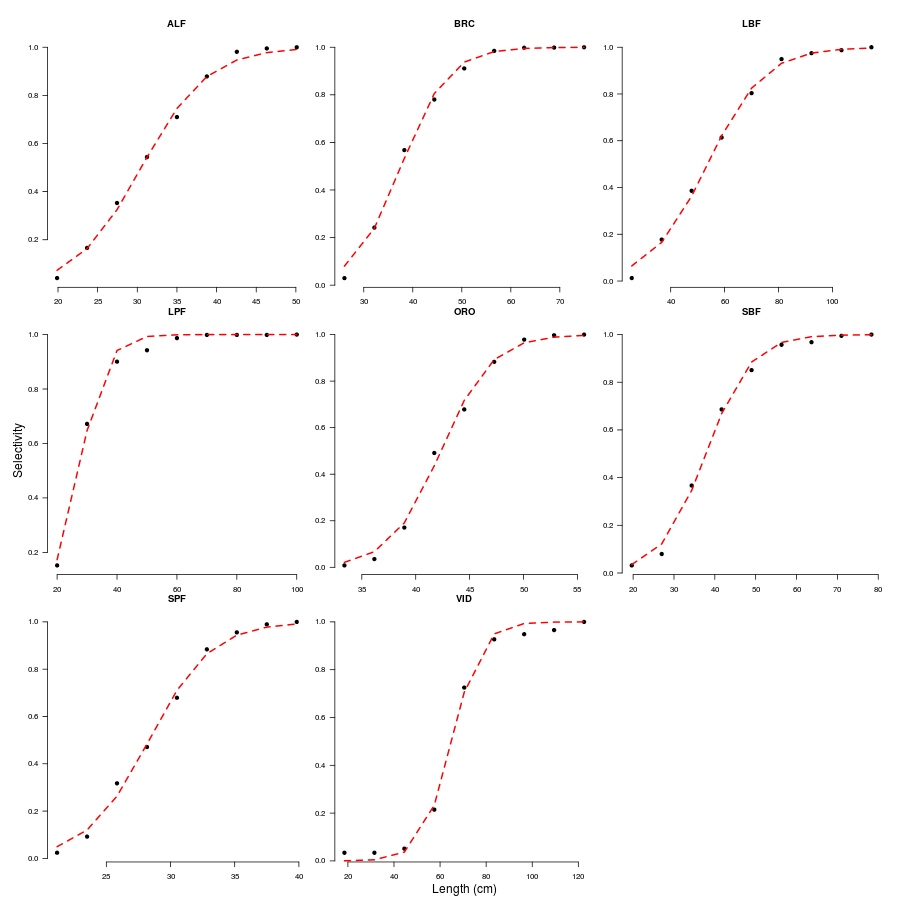
\includegraphics[width=.9\linewidth]{/home/demiurgo/Documents/PhD/Atlantis_Model/model_JFR/MandM/img/Selectivity.png}
\caption{Fishery gear Selectivity}
\end{figure}
\paragraph*{Effort}
\label{sec-5-2-2-4}

\begin{itemize}
\item I changed Catchability of lobster traps
\begin{itemize}
\item 50 to 30\% in Oct 1981
\begin{itemize}
\item 11596 days from the begening
\end{itemize}
\end{itemize}
\item Change in effort lobster fishery because of the chigre
\begin{itemize}
\item increase in a 47\% information based on Historic information
\begin{itemize}
\item 18262 days after begining (1-jun-2000)
\end{itemize}
\end{itemize}
\end{itemize}
\paragraph*{Swept area}
\label{sec-5-2-2-5}

\begin{itemize}
\item GCR and SPL
\begin{itemize}
\item I used the value reported by Ahumada 2009 fir the GCR. The total swep area affected by the trap is 54.4 m3
\end{itemize}
\item SPF
   The Volume of influence is 294 m3. whis is calculated from the distance of action of 5 meters away from the hook
\item LPG BRC and SBF LBF
\item ORO and ALF
\begin{itemize}
\item I using the trawling volumne
\item 40 meter of open
\item 10 meters high
\item 1000 m of trwling
\end{itemize}
\end{itemize}
\paragraph*{mFC}
\label{sec-5-2-2-6}

\begin{itemize}
\item Lobster
\begin{itemize}
\item The modeling day is assuming that the first day of simulation is 1919-01-17 to 1950-01-01 (burning period)
\end{itemize}
\end{itemize}

\begin{center}
\begin{tabular}{lrrrrl}
 Year         &     F(y-1)  &          u (d-1)  &      Total Change  &  Modeling day  &  Comment                   \\
\hline
 1900 - 1929  &   0.082085  &     0.0002248651  &                    &             0  &  First simulated years     \\
 1930 - 1979  &  0.4146949  &     0.0011355052  &      5.0497169644  &          4002  &  Early catch records       \\
 1980 - 1999  &  0.9152795  &     0.0025044736  &     11.1376703175  &         22264  &  Change Traps desig        \\
 2000 - 2009  &  0.8032620  &     0.0021982979  &      9.7760735648  &         29204  &  Use of Chigre             \\
 2010 - 2015  &     0.8434  &  0.0023080173541  &  10.2640076092654  &         33222  &  Increase number of Boats  \\
\end{tabular}
\end{center}



\begin{itemize}
\item The modeling day is assuming that the first day of simulation is 1950-01-01 (NO burning period)
\end{itemize}

\begin{center}
\begin{tabular}{lrrrrl}
 Year         &     F(y-1)  &          u (d-1)  &      Total Change  &  Modeling day  &  Comment                   \\
\hline
 1900 - 1929  &   0.082085  &     0.0002248651  &                    &             0  &  First simulated years     \\
 1930 - 1979  &  0.4146949  &     0.0011355052  &      5.0497169644  &          4002  &  Early catch records       \\
 1980 - 1999  &  0.9152795  &     0.0025044736  &     11.1376703175  &         22264  &  Change Traps desig        \\
 2000 - 2009  &  0.8032620  &     0.0021982979  &      9.7760735648  &         29204  &  Use of Chigre             \\
 2010 - 2015  &     0.8434  &  0.0023080173541  &  10.2640076092654  &         33222  &  Increase number of Boats  \\
\end{tabular}
\end{center}




\begin{itemize}
\item GCR
\end{itemize}

\begin{center}
\begin{tabular}{lrrl}
 Year         &  F(y - 1)  &        u (d - 1)  &  Source                  \\
\hline
 2005 - 2006  &      0.05  &  0.0001369769192  &  Ahumada and Arana 2009  \\
\end{tabular}
\end{center}



\begin{itemize}
\item ORO
\end{itemize}

\begin{center}
\begin{tabular}{rrrrrl}
 Year  &            U  &          1-U  &        U(d-1)  &    Proportion  &  Comment    \\
\hline
 1999  &  0.050855086  &  0.949144914  &  0.0001429865  &             1  &  Paya 2013  \\
 2000  &  0.090519052  &  0.909480948  &  0.0002599148  &  1.8177580257  &             \\
 2001  &  0.166786679  &  0.833213321  &  0.0004997808  &  3.4953013371  &             \\
 2002  &  0.174917492  &  0.825082508  &  0.0005266336  &  3.6831009597  &             \\
 2003  &  0.142364236  &  0.857635764  &  0.0004206671  &  2.9420063262  &             \\
 2004  &  0.189138914  &  0.810861086  &   0.000574242  &  4.0160584055  &             \\
 2005  &  0.118991899  &  0.881008101  &  0.0003470314  &  2.4270230275  &             \\
 2006  &  0.055925593  &  0.944074407  &  0.0001576596  &  1.1026191513  &             \\
 2007  &  0.002040204  &  0.997959796  &    5.595E-006  &  0.0391316352  &             \\
\end{tabular}
\end{center}




\begin{itemize}
\item ALF (Wiff 2012 report)
\end{itemize}

\begin{center}
\begin{tabular}{rrrrl}
 Year  &      F(y-1)  &   u (d-1)  &          Change  &  Comment  \\
\hline
 1998  &  0.00240024  &  0.000007  &               1  &           \\
 1999  &  0.01910191  &  0.000052  &    7.9581512576  &           \\
 2000  &  0.19381938  &  0.000531  &   80.7288296206  &           \\
 2001  &  0.29182918  &  0.000799  &  121.5351410082  &           \\
 2002  &  0.90669067  &  0.002481  &  377.2824515462  &           \\
 2003  &   0.3540354  &  0.000969  &  147.4289733182  &           \\
 2004  &  0.53585359  &  0.001467  &  223.0869420642  &           \\
 2005  &  0.40194019  &  0.001101  &  167.3667144086  &           \\
 2006  &  0.44014401  &  0.001205  &  183.2650834303  &           \\
 2007  &  0.62916292  &  0.001722  &   261.900078148  &           \\
 2008  &  0.27992799  &  0.000767  &  116.5806733744  &           \\
 2009  &  0.08610861  &  0.000236  &   35.8708865686  &           \\
\end{tabular}
\end{center}


\begin{itemize}
\item Other Functional groups
\end{itemize}
These estimation are based on the observed catch and the simulated biomass

\begin{center}
\begin{tabular}{lrrrrrr}
 FG   &  Sim Bio  &         Catch  &             U  &                      F  &              mFC  &     After Burning  \\
\hline
 ANG  &     7000  &          13.3  &        0.9981  &           0.0019018073  &  0.0000052104174  &  0.00000053297649  \\
 BRC  &     4800  &          10.4  &  0.9978333333  &           0.0021690173  &  0.0000059424955  &  0.00000060786116  \\
 BRC  &     4800  &           8.3  &  0.9982708333  &           0.0017306634  &  0.0000047415323  &  0.00000048501398  \\
 LBF  &    10000  &  0.7395930529  &  0.9999260407  &            0.000073962  &  0.0000002026357  &  0.00000002072772  \\
 LPF  &     6450  &          10.2  &  0.9984186047  &           0.0015826471  &  0.0000043360100  &  0.00000044353287  \\
 OCT  &      400  &  9.9921565045  &  0.9750196087  &           0.0252976967  &  0.0000693063562  &  0.00000708938570  \\
 SBF  &    10000  &  0.4992841908  &  0.9999500716  &  4.99296655439205E-005  &  0.0000001367936  &  0.00000001399269  \\
 SPF  &     5200  &  0.7702600404  &  0.9998518731  &           0.0001481379  &  0.0000004058572  &  0.00000004151536  \\
 VID  &     3200  &  1.1453337032  &  0.9996420832  &           0.0003579808  &  0.0000009807690  &  0.00000010032340  \\
 GCR  &           &                &                &                   0.05  &  0.0001369769192  &                    \\
\end{tabular}
\end{center}
\paragraph*{Total Bait Catch}
\label{sec-5-2-2-7}

\begin{itemize}
\item To get the total bait catch I extrapolate the values of catch per trip to the total of trips by season.
\begin{itemize}
\item I used the catch per trip from the Data base
\item The trips per season where obtained from the Marine traphic control logbook.
\end{itemize}
\item I added the information from the Juan Fernandez fisheries report year 2016, the TOtal catch and by catch reported there.
\end{itemize}

\begin{center}
\begin{tabular}{lrrrr}
      &  CPT-SPL  &         &  CPT-GCR  &  Total (tons)  \\
\hline
      &       AS  &  RC-SC  &    RC-SC  &                \\
 ANG  &    26414  &  33199  &     3008  &        62.621  \\
 BRC  &    30038  &  55301  &     1651  &         86.99  \\
 JUR  &    15420  &  74002  &     1752  &        91.174  \\
 VID  &    19912  &  56152  &     3016  &         79.08  \\
\end{tabular}
\end{center}




\begin{verbatim}
rm(list = ls())
library(ascii)
options(asciiType = "org")
library(ggplot2)
source('/home/demiurgo/Documents/PhD/Atlantis_Model/tools/General_tools/Atlantis_tools.R')
## Reading data
#lc     <- read.csv('/home/demiurgo/Documents/PhD/Harvest/catch.sp/Location_catches_fgs.csv')
lc     <- read.csv('/home/demiurgo/Documents/PhD/Harvest/catch.sp/CpT.csv')
lc <- lc[lc$Year>2010,]
tr     <- read.csv('/home/demiurgo/Documents/PhD/Harvest/catch.sp/trips_by_season.csv')
weight <- read.csv('/home/demiurgo/Documents/PhD/Harvest/catch.sp/weight.csv')
##~ FUNCTIONAL GROUPS
lc    <- FG(data = lc, column = 5)
##
##~ By season
lc$Season <- with(lc,  ifelse(Mes %in% c(1, 2, 3), 1, ifelse(Mes %in% c(4, 5, 6), 2,
                                                        ifelse(Mes %in% c(7, 8, 9), 3, 4))))
tr$Season <- with(tr,  ifelse(Month %in% c(1, 2, 3), 1, ifelse(Month %in% c(4, 5, 6), 2,
                                                        ifelse(Month %in% c(7,8,9),   3, 4))))
## Total number of trips by Year (Information from the marine trafic control)
tr        <- na.omit(tr)        #  Remove Empty rows
## Numbre of trips
png('img/Catch_per_trip.png', height = 900, width = 900)
p <- ggplot(tr, aes(x=factor(Month), y=trips, group=as.factor(Year))) + geom_line(aes(color=as.factor(Year)),size=2) + facet_wrap(~Island,ncol=2)
p <- p+scale_color_brewer(palette="Reds")+theme_minimal()+ labs(y = 'Tripts per Month',x='Month',colour = "Years")
p
invisible(dev.off())
## trips
glob.trip <- by(tr$trips, list(tr$Year, tr$Island, tr$Season), sum, na.rm = TRUE)
trip      <- data.frame(Year   = with(tr, rep(unique(Year), length(unique(Island)) * length(unique(Season)))),
                        Season = with(tr, sort(rep(unique(Season), length(unique(Year)) * length(unique(Island))))),
                        Island = with(tr, rep(sort(rep(unique(Island), length(unique(Year)))), length(unique(Season)))),
                        trips  = do.call(rbind,  as.list(glob.trip)))
## Total trips per Season and Island
t.trip <- na.omit(trip)
## Functional groups bait cahtch
lc    <- na.omit(lc)        #  Remove Empty rows
lc.FG <- split(lc, paste(lc$Year, lc$Island))
## list of catch per trip by season and by FG
CpT         <- as.data.frame(do.call(rbind, lapply(lc.FG, sumry)), rownames = FALSE)
CpT$TC.numb <- NA
for(i in 1 : nrow(t.trip)){
    post              <- which(CpT$Year == t.trip$Year[i] & CpT$Season == t.trip$Season[i] & CpT$Island == t.trip$Island[i])
    CpT$TC.numb[post] <- CpT$cperT[post] * t.trip$trips[i] /1000
}
## CpT$TC.weight <- NA
## for( i in 1 : nrow(weight)){
##     post                  <- which(CpT$FG %in%weight$FG[i])
##     CpT$TC.weight[post]   <- CpT$TC.numb[post] * weight$weight[i]  / 1000000 # passing direct to tonnes
## }
## CAtch per season
CpT <- na.omit(CpT)
png('img/Catch_per_Season.png', height = 1000, width = 1000)
sp <- ggplot(data = CpT, aes(Season, TC.numb, group = as.factor(Year))) + geom_line (aes(color=as.factor(Year)), size=2)#geom_point() + geom_smooth(method = "lm", color = 'red')
sp + facet_wrap(~FG + Island, ncol = 4, scales = 'free_y')
#sp
invisible(dev.off())
## Catch per Year and island
tmp   <- lapply(split(CpT, paste(CpT$Year, CpT$Island, CpT$FG)), function(x) sum(x$TC.numb))
cat.w <- data.frame(matrix(unlist(strsplit(names(tmp), ' ')), ncol = 3, byrow = TRUE))
cat.w$Catch.W <- c(unlist(tmp))
colnames(cat.w)[1 : 3] <- c('Year', 'Island', 'FG')
png('img/Catch_per_Year_Island.png', height = 1000, width = 1000)
sp <- ggplot(data = cat.w, aes(Year, Catch.W, group = 1))+ geom_point() + geom_smooth(method = "lm", color = 'red')
sp + facet_wrap(~FG + Island, ncol = 4, scales = 'free_y')
invisible(dev.off())
## Total Catch per year
cat.w <- na.omit(cat.w)
tmp <- lapply(split(cat.w, paste(cat.w$Year, cat.w$FG)), function(x) sum(x$Catch.W))
catch.year <- data.frame(matrix(unlist(strsplit(names(tmp), ' ')), ncol = 2, byrow = TRUE))
catch.year$Total <- c(unlist(tmp))
colnames(catch.year)[1 : 2] <- c('Year', 'FG')
png('img/Total_Catch_per_Year.png', height = 1000, width = 1000)
sp <- ggplot(data = catch.year, aes(Year, Total, group = 1))+ geom_line() #+ geom_smooth(method = "lm", color = 'red')
sp + facet_wrap(~FG , ncol = 4, scales = 'free_y')
invisible(dev.off())
catch.year <- catch.year[order(catch.year$FG, catch.year$Year), ]
tab.out <- xtabs(Total ~ FG + Year, catch.year)
cap1    <- 'Catch of bait by years'
b       <- ascii(tab.out, header=T,  include.rownames = TRUE, include.colnames = T, caption = cap1)
print(b)
write.table(catch.year, '/home/demiurgo/Documents/PhD/Harvest/catch.sp/catch.csv')
\end{verbatim}

\begin{center}
\begin{tabular}{llrrrrrr}
              &       &  \textbf{Year}  &         &         &         &         &         \\
              &       &           2011  &   2012  &   2013  &   2014  &   2015  &   2016  \\
\hline
 \textbf{FG}  &  ANG  &           6.88  &  25.30  &  27.98  &  43.21  &  38.00  &   9.50  \\
              &  BRC  &          10.06  &  35.12  &  47.17  &  53.00  &  56.97  &  21.73  \\
              &  CHO  &           0.10  &   0.17  &   0.07  &   0.70  &   0.03  &   0.00  \\
              &  GCR  &           0.00  &   0.00  &   0.00  &   0.00  &   0.00  &   0.00  \\
              &  LBF  &           0.11  &   0.86  &   0.97  &   2.00  &   0.43  &   0.52  \\
              &  LPF  &           2.52  &  14.93  &  15.76  &  21.97  &  14.21  &  11.63  \\
              &  OCT  &           0.00  &   0.03  &   0.13  &   0.18  &   0.37  &   0.85  \\
              &  SBF  &           0.34  &   0.86  &   0.75  &   0.68  &   2.90  &   0.55  \\
              &  SPF  &           0.11  &   0.74  &   0.96  &   2.25  &   1.40  &   1.70  \\
              &  VID  &           0.36  &   2.56  &   4.22  &   4.50  &   4.40  &   6.51  \\
\end{tabular}
\end{center}


 \begin{figure}[htb]
 \centering
 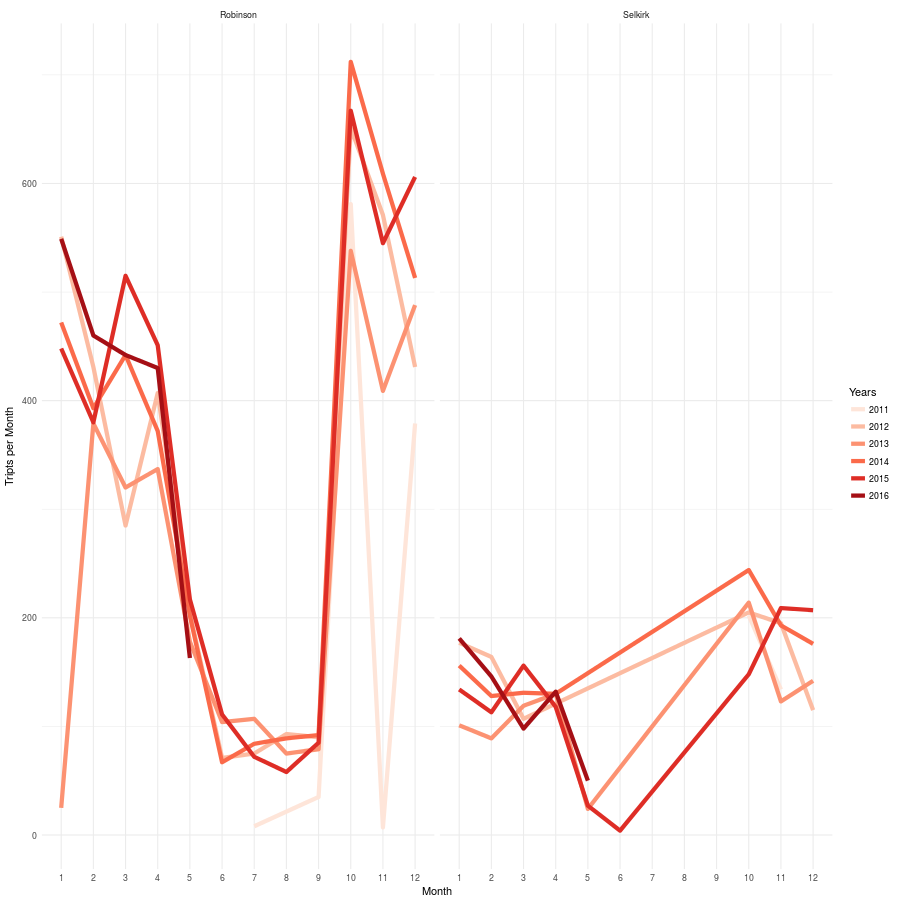
\includegraphics[width=.9\linewidth]{/home/demiurgo/Documents/PhD/Atlantis_Model/model_JFR/MandM/img/Catch_per_trip.png}
 \caption{Trips by Month}
 \end{figure}
 \begin{figure}[htb]
 \centering
 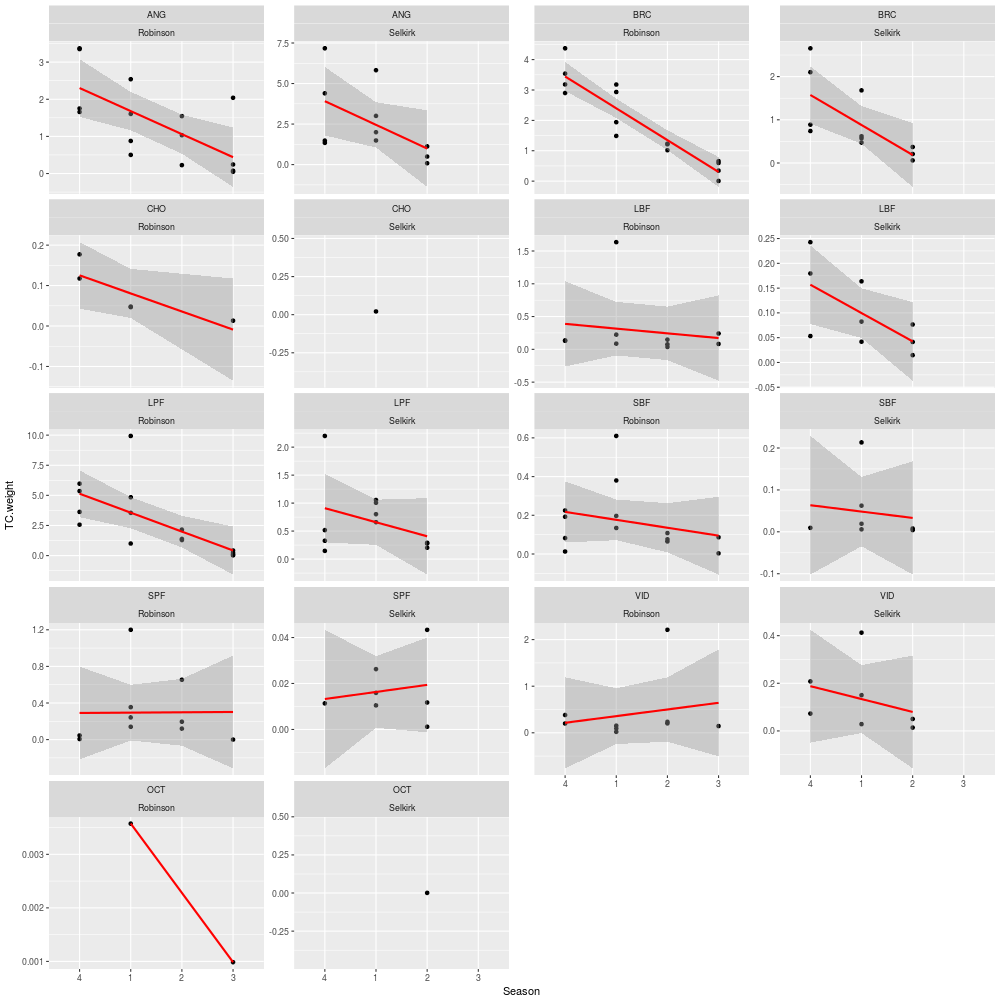
\includegraphics[width=.9\linewidth]{/home/demiurgo/Documents/PhD/Atlantis_Model/model_JFR/MandM/img/Catch_per_Season.png}
 \caption{Bait catch per season}
 \end{figure}
 \begin{figure}[htb]
 \centering
 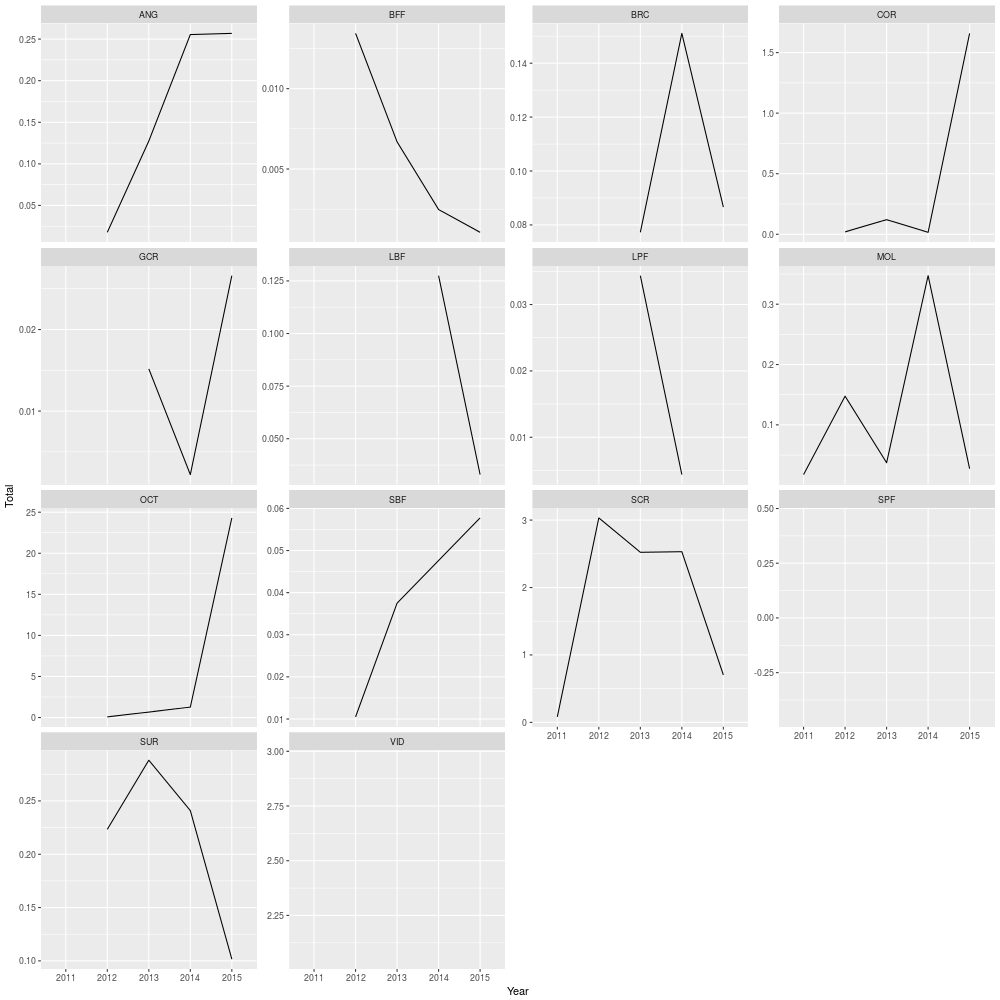
\includegraphics[width=.9\linewidth]{/home/demiurgo/Documents/PhD/Atlantis_Model/model_JFR/MandM/img/Total_Catch_per_Year.png}
 \caption{Bait catch per year and Island}
 \end{figure}
\paragraph*{Bycatch and Discars}
\label{sec-5-2-2-8}
\begin{itemize}

\item Discards
\label{sec-5-2-2-8-1}%
\begin{itemize}

\item Industrial
\label{sec-5-2-2-8-1-1}%
\begin{itemize}
\item Cada tonelada de descarte se tiene una tonelada de peces de desembarcados \cite{yAñes 2008}
\begin{itemize}
\item Has effect on Coral ans sesils epifauna
\end{itemize}
\item The 98.85\% of the catch per tow correspond to Rorange roughy (The rest are fishes)
\begin{itemize}
\item almost the 11 \% of the catch is coral (But decrease with time) \cite{Anderson2003}
\begin{itemize}
\item Other species 1.3 \% (This can be BFF)
\item Species like CHo can be almost the 0.2\% of the catch
\end{itemize}
\end{itemize}
\item The 98.96\% of the catch per tow correspond to alfosnino (The rest are fishes)
\end{itemize}

\item Artisanal
\label{sec-5-2-2-8-1-2}%
\begin{itemize}
\item To stimate te total bycatch I used the same approach that one used for the estimation of bait catch
\item I multiply the number of trips by the bycatch per trips
\item For the YEar 2016 I used the estimation from the report: Fisheries of Juan Fernandez year 2016.
\end{itemize}
\begin{table}[htb]
\caption{Total Bait catch per year in the JFRE}
\begin{center}
\begin{tabular}{lrrrr}
 FG   &        &        &  Indi. Weight  &  Total (Ton)  \\
\hline
 OCT  &  1632  &  3627  &          0.64  &      3.36576  \\
 SCR  &  7445  &  3203  &          0.52  &      5.53696  \\
 COR  &   338  &    35  &             1  &        0.373  \\
\end{tabular}
\end{center}
\end{table}




\begin{verbatim}
rm(list = ls())
library(ascii)
options(asciiType = "org")
library(ggplot2)
source('/home/demiurgo/Documents/PhD/Atlantis_Model/tools/General_tools/Atlantis_tools.R')
## Reading data
lc     <- read.csv('/home/demiurgo/Documents/PhD/Harvest/catch.sp/Bycatch/Bycatch.csv')
tr     <- read.csv('/home/demiurgo/Documents/PhD/Harvest/catch.sp/trips_by_season.csv')
weight <- read.csv('/home/demiurgo/Documents/PhD/Harvest/catch.sp/Bycatch/weight.csv')
##~ FUNCTIONAL GROUPS
lc    <- FG(data = lc, column = 6)
lc    <- na.omit(lc)        #  Remove Empty rows
##
##~ By season
lc$Season <- with(lc,  ifelse(Month %in% c(1, 2, 3), 1, ifelse(Month %in% c(4, 5, 6), 2,
                                                        ifelse(Month %in% c(7, 8, 9), 3, 4))))
tr$Season <- with(tr,  ifelse(Month %in% c(1, 2, 3), 1, ifelse(Month %in% c(4, 5, 6), 2,
                                                        ifelse(Month %in% c(7,8,9),   3, 4))))
## get everything in numbers
w.pos <- which(lc$Units %in% c('p', 'P'))
for( w in w.pos){
    fg.pos       <- which(weight$FG %in% lc$FG[w])
    lc$Volume[w] <- lc$Volume[w] / weight$weight[fg.pos]
    if(is.na(lc$Volume[w])) stop( lc$FG[w])
}
## Total number of trips by Year (Information from the marine trafic control)
tr        <- na.omit(tr)        #  Remove Empty rows
glob.trip <- by(tr$trips, list(tr$Year, tr$Island, tr$Season), sum, na.rm = TRUE)
trip      <- data.frame(Year   = with(tr, rep(unique(Year), length(unique(Island)) * length(unique(Season)))),
                        Season = with(tr, sort(rep(unique(Season), length(unique(Year)) * length(unique(Island))))),
                        Island = with(tr, rep(sort(rep(unique(Island), length(unique(Year)))), length(unique(Season)))),
                        trips  = do.call(rbind,  as.list(glob.trip)))
## Total trips per Season and Island
t.trip <- na.omit(trip)
lc$Total_unit <- lc$Volume
## Functional groups bait cahtch
lc.FG <- split(lc, paste(lc$Year, lc$Island))
## list of catch per trip by season and by FG
CpT         <- as.data.frame(do.call(rbind, lapply(lc.FG, sumry)), rownames = FALSE)
CpT$TC.numb <- NA
for(i in 1 : nrow(t.trip)){
    post              <- which(CpT$Year == t.trip$Year[i] & CpT$Season == t.trip$Season[i] & CpT$Island == as.character(t.trip$Island[i]))
    CpT$TC.numb[post] <- CpT$cperT[post] * t.trip$trips[i]
}
CpT$TC.weight <- NA
for( i in 1 : nrow(weight)){
    post                  <- which(CpT$FG %in% weight$FG[i])
    CpT$TC.weight[post]   <- CpT$TC.numb[post] * weight$weight[i]  / 1000000 # passing direct to tonnes
}
## CAtch per season
CpT <- na.omit(CpT)
png('img/Bycatch_per_Season.png', height = 1000, width = 1000)
sp <- ggplot(data = CpT, aes(Season, TC.weight, group = 1))+ geom_point() + geom_smooth(method = "lm", color = 'red')
sp + facet_wrap(~FG + Island, ncol = 4, scales = 'free_y')
#sp
invisible(dev.off())
## Catch per YEar and island
tmp   <- lapply(split(CpT, paste(CpT$Year, CpT$Island, CpT$FG)), function(x) sum(x$TC.weight))
cat.w <- data.frame(matrix(unlist(strsplit(names(tmp), ' ')), ncol = 3, byrow = TRUE))
cat.w$Catch.W <- c(unlist(tmp))
colnames(cat.w)[1 : 3] <- c('Year', 'Island', 'FG')
png('img/Bycatch_per_Year_Island.png', height = 1000, width = 1000)
sp <- ggplot(data = cat.w, aes(Year, Catch.W, group = 1))+ geom_point() + geom_smooth(method = "lm", color = 'red')
sp + facet_wrap(~FG + Island, ncol = 4, scales = 'free_y')
#sp
invisible(dev.off())
## Total Catch per year
cat.w <- na.omit(cat.w)
tmp <- lapply(split(cat.w, paste(cat.w$Year, cat.w$FG)), function(x) sum(x$Catch.W))
catch.year <- data.frame(matrix(unlist(strsplit(names(tmp), ' ')), ncol = 2, byrow = TRUE))
catch.year$Total <- c(unlist(tmp))
colnames(catch.year)[1 : 2] <- c('Year', 'FG')
png('img/Total_Bycatch_per_Year.png', height = 1000, width = 1000)
sp <- ggplot(data = catch.year, aes(Year, Total, group = 1))+ geom_line() #+ geom_smooth(method = "lm", color = 'red')
sp + facet_wrap(~FG , ncol = 4, scales = 'free_y') + labs(y = 'Total catch [Tons]', x = 'Years')
#sp
invisible(dev.off())
catch.year <- catch.year[order(catch.year$FG, catch.year$Year), ]
tab.out <- xtabs(Total ~ FG + Year, catch.year)
write.table(catch.year, '/home/demiurgo/Documents/PhD/Harvest/catch.sp/Bycatch/Bycatch_out.csv')
cap    <- 'Total Bycatch Tons per Year'
c       <- ascii(tab.out, header=T,  include.rownames = TRUE, include.colnames = T, caption = cap)
print(c)
\end{verbatim}

\begin{center}
\begin{tabular}{llrrrrr}
              &       &  \textbf{Year}  &        &        &        &        \\
              &       &           2011  &  2012  &  2013  &  2014  &  2015  \\
\hline
 \textbf{FG}  &  BFF  &           0.00  &  0.01  &  0.01  &  0.00  &  0.00  \\
              &  COR  &           0.00  &  0.02  &  0.12  &  0.02  &  0.59  \\
              &  MOL  &           0.02  &  0.15  &  0.04  &  0.26  &  0.03  \\
              &  OCT  &           0.00  &  0.08  &  0.69  &  1.34  &  1.54  \\
              &  SCR  &           0.08  &  3.05  &  2.71  &  2.71  &  0.82  \\
              &  SUR  &           0.00  &  0.23  &  0.31  &  0.26  &  0.12  \\
\end{tabular}
\end{center}



 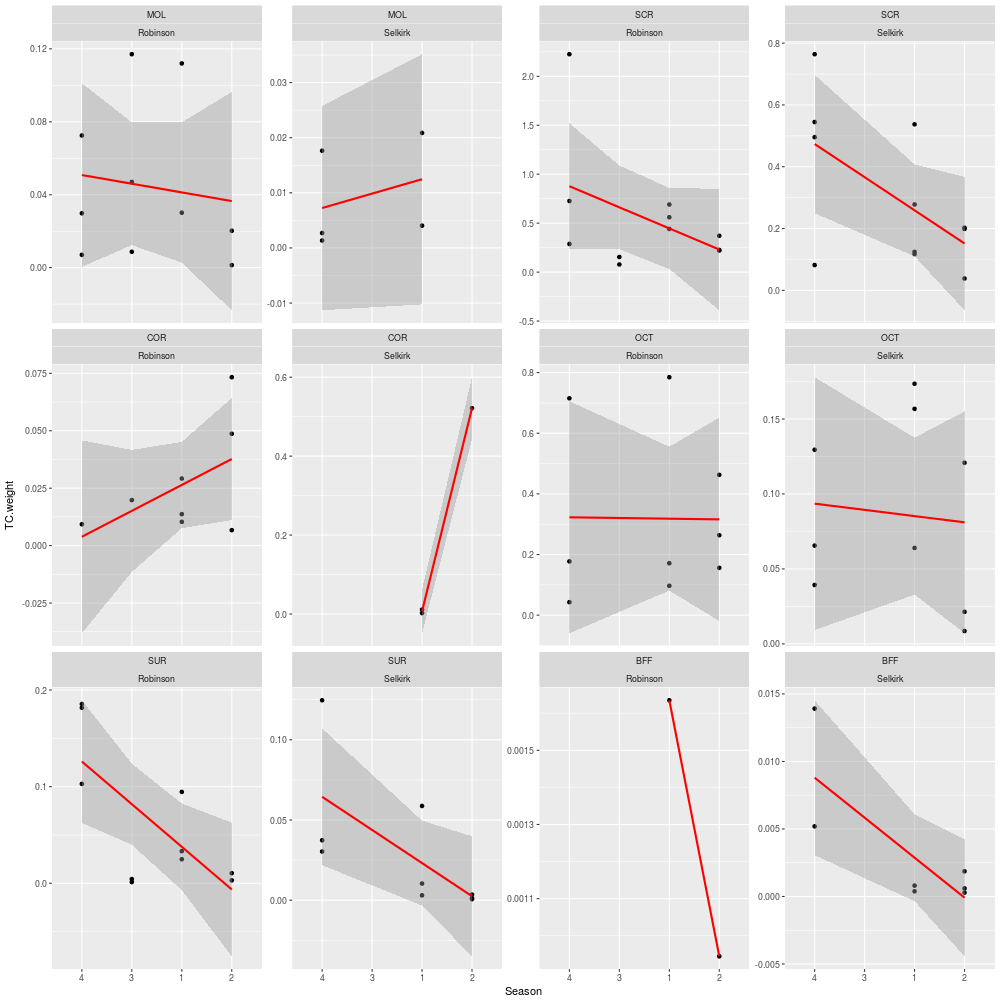
\includegraphics[width=.9\linewidth]{/home/demiurgo/Documents/PhD/Atlantis_Model/model_JFR/MandM/img/Bycatch_per_Season.png}
 \begin{figure}[htb]
 \centering
 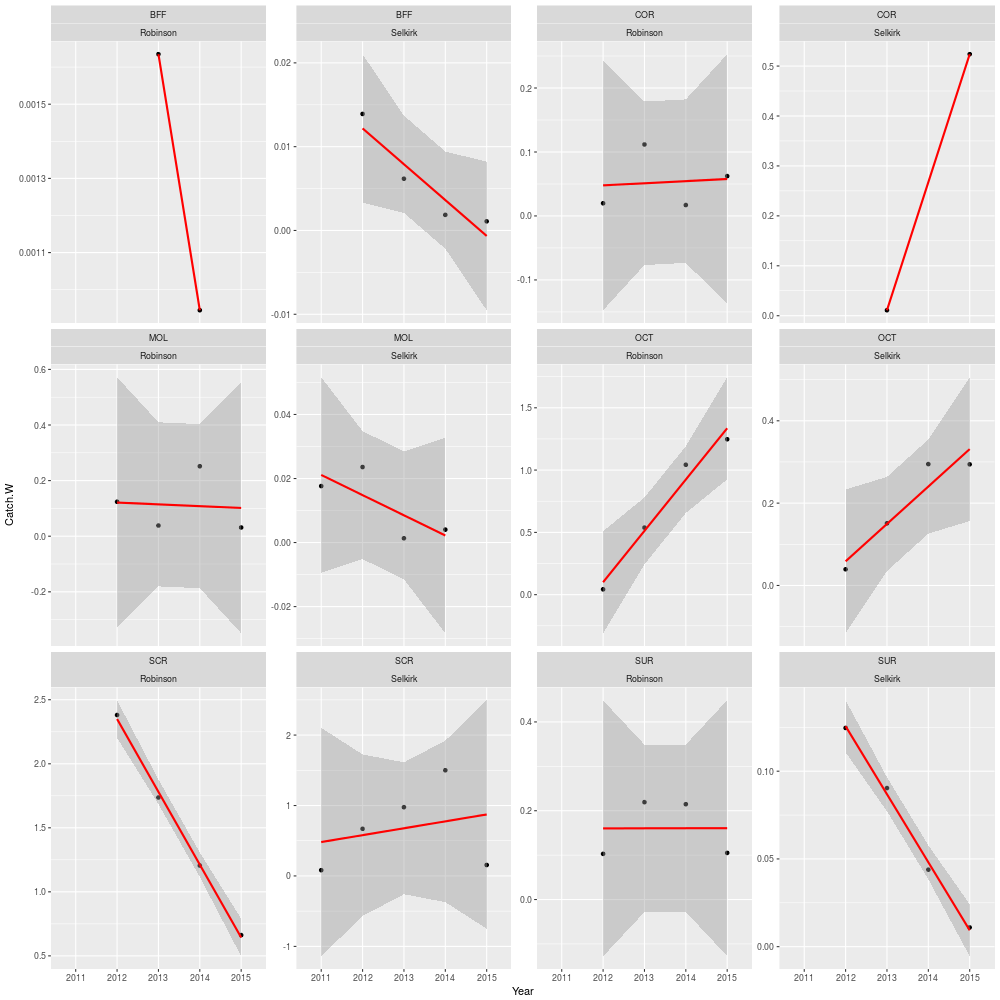
\includegraphics[width=.9\linewidth]{/home/demiurgo/Documents/PhD/Atlantis_Model/model_JFR/MandM/img/Bycatch_per_Year_Island.png}
 \caption{Bait catch per season}
 \end{figure}
 \begin{figure}[htb]
 \centering
 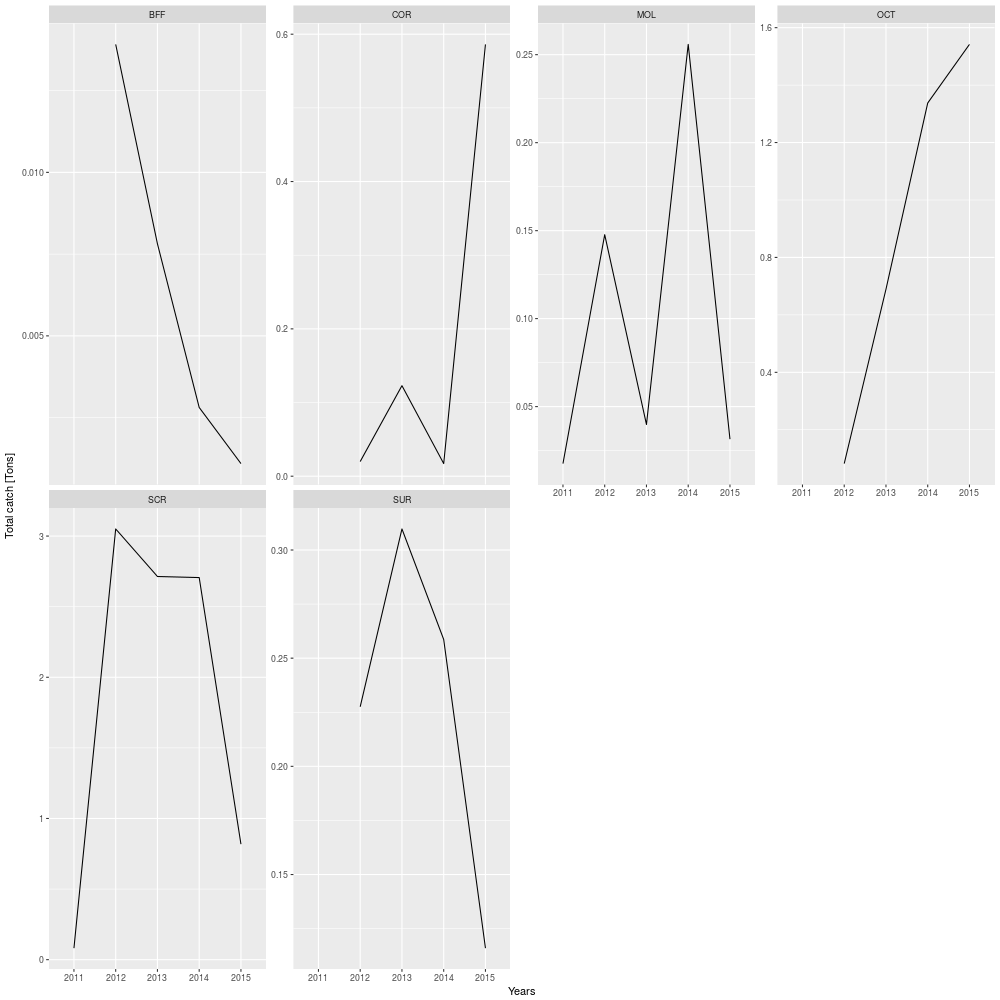
\includegraphics[width=.9\linewidth]{/home/demiurgo/Documents/PhD/Atlantis_Model/model_JFR/MandM/img/Total_Bycatch_per_Year.png}
 \caption{Bait catch per year and Island}
 \end{figure}
\end{itemize} % ends low level
\end{itemize} % ends low level
\subsubsection*{Solar radiation}
\label{sec-5-2-3}

\begin{itemize}
\item I se the information irradiance from \href{http://www.soda-pro.com/web-services/radiation/nasa-sse}{soda}
\item The model use rewind of the data
\end{itemize}
\subsection*{Forcing files}
\label{sec-5-3}
\subsubsection*{Rain}
\label{sec-5-3-1}
\paragraph*{Reconstruction of the TS}
\label{sec-5-3-1-1}

\begin{itemize}
\item I wil use the information form the `Anuarios climatologicos' from the \textbf{DIRECCIÓN GENERAL DE AERONÁUTICA CIVIL}
\item This data has some gaps to I will reconstruc the data usind diferent model
\begin{itemize}
\item Due to the similaity with the original time series I will use new time series from the ARIMA model and from the SPLINE

\begin{verbatim}
## Wavelet descomposition and time serie recontruction
library(imputeTS)
source('/home/demiurgo/Documents/PhD/Atlantis_Model/tools/Atlantis_tools.R')
dat   <- read.csv('/home/demiurgo/Documents/PhD/Forcing_Files/NO3/NO3.csv')
dates <- as.Date(as.Date(dat[,4]), format = '%Y/%m/%d')
## remove trend in the data
lmodel  <- predict(lm(Precipitation ~ day, data = dat, na.action = na.exclude), data.frame(day = dat$day))
ts.pres <- dat[, 5] - lmodel
## By interpolation
## ~~~~~~~~~~~~~~~~~~~~~
## Spline interpolation
spline <- na.interpolation(ts.pres, option = 'spline')
## Linear interpolation
linear <- na.interpolation(ts.pres, option = 'linear')
## Linear interpolation
stine  <- na.interpolation(ts.pres, option = 'stine')
## By Kalman Smoothing and State Space Models
## ~~~~~~~~~~~~~~~~~~~~~~~~~~~~~~~~~~~~~~~~~~
## Structural model fitted by maximum likelihood
like   <- na.kalman(ts.pres, model = "StructTS", smooth = TRUE, nit = -1)
## State space representation of arima mode
arima  <- na.kalman(ts.pres, model = "auto.arima", smooth = TRUE, nit = -1)
## State space representation of arima mode
like.t <- na.kalman(ts.pres, model = "StructTS", smooth = TRUE, type = 'trend')
## Back data to original magnitud Using the total by month.
lmodel[is.na(lmodel)] <- 0
spline  <- spline + lmodel
linear  <- linear + lmodel
stine   <- stine + lmodel
like    <- like + lmodel
arima   <- arima + lmodel
like.t  <- like.t + lmodel
ts.pres <- dat[, 5]
## Plotting outputs
## ~~~~~~~~~~~~~~~~~~
png('/home/demiurgo/Documents/PhD/Atlantis_Model/model_JFR/MandM/img/Rain.png', width = 900, height = 900)
par(mfrow = c(2, 1), oma = c(1, 1, 1, 1), mar = c(1, 5, 1, 1))
plot(dates, spline, col = 'royalblue', type = 'l', ylab = 'Precipitacion', xlab = 'Date', xaxt='n')
lines(dates, linear, col = 'firebrick')
lines(dates, stine, col = 'darkolivegreen')
lines(dates, ts.pres, type = 'l', col = 1)
legend('topleft', legend = c('Original', 'Spline', 'Linear', 'Stine'),
       col = c('black', 'royalblue', 'firebrick', 'darkolivegreen'), lty = 1, bty = 'n')
plot(dates, like, col = 'darkolivegreen', type = 'l', ylab = 'Precipitacion', xlab = 'Date')
lines(dates, arima, col = 'royalblue')
lines(dates, ts.pres, type = 'l')
legend('topleft', legend = c('Original', 'ARIMA', 'Likelihood'),
       col = c('black', 'royalblue', 'darkolivegreen'), lty = 1, bty = 'n')
dev.off()
## Savind data
## ~~~~~~~~~~~~~
dat$spline <- spline
dat$arime  <- arima
dat$date   <- dates
write.table(dat, file = '/home/demiurgo/Documents/PhD/Forcing_Files/NO3/Rain.csv', row.names = FALSE)
\end{verbatim}
\end{itemize}
\begin{figure}[htb]
  \centering
  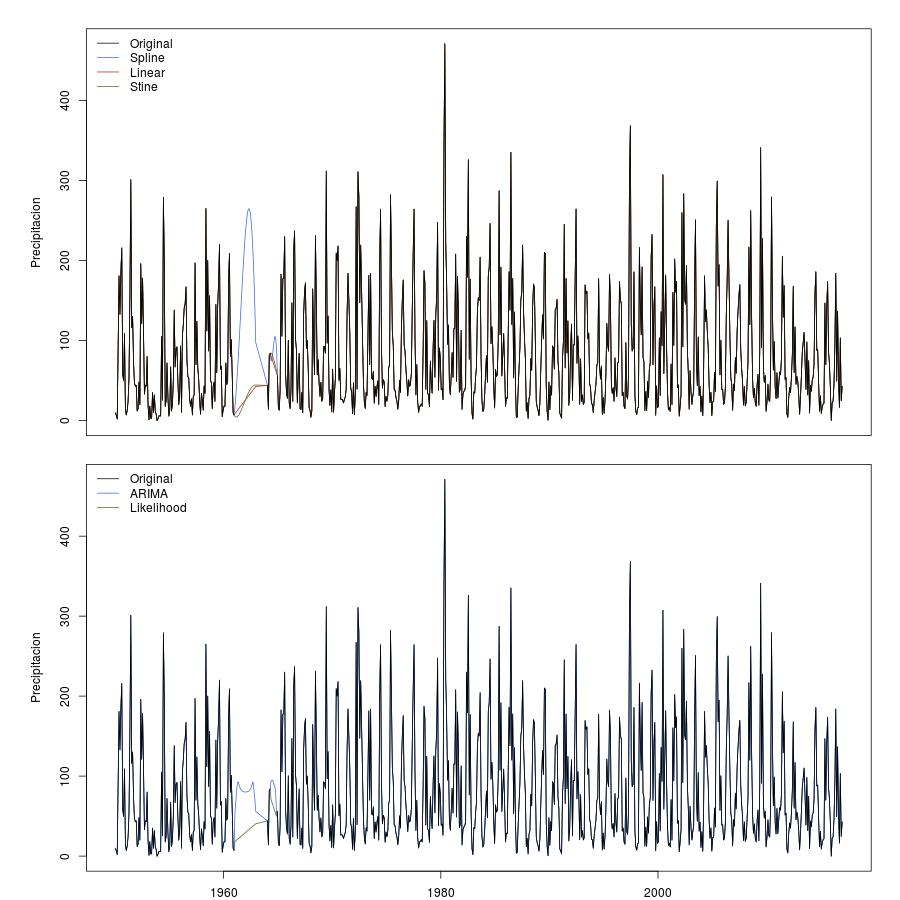
\includegraphics[width=.9\linewidth]{/home/demiurgo/Documents/PhD/Atlantis_Model/model_JFR/MandM/img/Rain.png}
  \caption{Total Bait catch per year in the JFRE}
  \end{figure}
\end{itemize}
\paragraph*{Localization of the river}
\label{sec-5-3-1-2}

\begin{itemize}
\item To locate the river and the ridge that support most of the water affluents,  I used the rivers of Selkirk (Masoli 2008) and Robinson (Astudillo,  2014)
\begin{itemize}
\item due to the effect of intense rain I decide to analize the effect of alluvium,  something that happend in intense rains (Masoli 2008). For that I use the percentile on 90\%,  so event higher that taht would be event of extreme rain
\end{itemize}
\end{itemize}

\begin{verbatim}
## extream rain events
 ## Read data
 dat <- read.csv(file = '/home/demiurgo/Documents/PhD/Forcing_Files/NO3/1-Rain.csv', sep = ' ')
 png('/home/demiurgo/Documents/PhD/Atlantis_Model/model_JFR/MandM/img/Rain_extreme.png', width = 900, height = 400)
 plot(dat$arima, type = 'l', yaxt = 'n', xaxt = 'n', ylab = 'Rainfall (mm)', xlab = 'Date', bty = 'n')
 tickx <- seq(from = 1, to = length(dat$date), length = 5)
 yticks <- seq(0, max(dat$arima), by = round(max(dat$arima) / 5))
 abline(h = quantile(dat$arima,c(.9)), col = 'firebrick', lty = 2, lwd = 1.5)
 abline(h = mean(dat$arima), col = 'goldenrod', lty = 2, lwd = 1.5)
 axis(2, at = yticks , labels = yticks, lwd = 2,  col = 1, las = 1)
 axis(1, at = dat$date[tickx], labels = format.Date(dat$date[tickx], '%Y.%m'), lwd = 2,  col = 1)
 legend('topleft', c('Average', '9th percentile'), col = c('goldenrod', 'firebrick'),
        lty = c(2, 2),  bty = 'n')
 dev.off()
 dat$a.extreme <- dat$arima
 dat$a.extreme[which(dat$a.extreme < quantile(dat$arima,c(.9)))] <- NA
 write.table(dat, file = '/home/demiurgo/Documents/PhD/Forcing_Files/NO3/2-Rain_extrem.csv', row.names = FALSE)
\end{verbatim}
     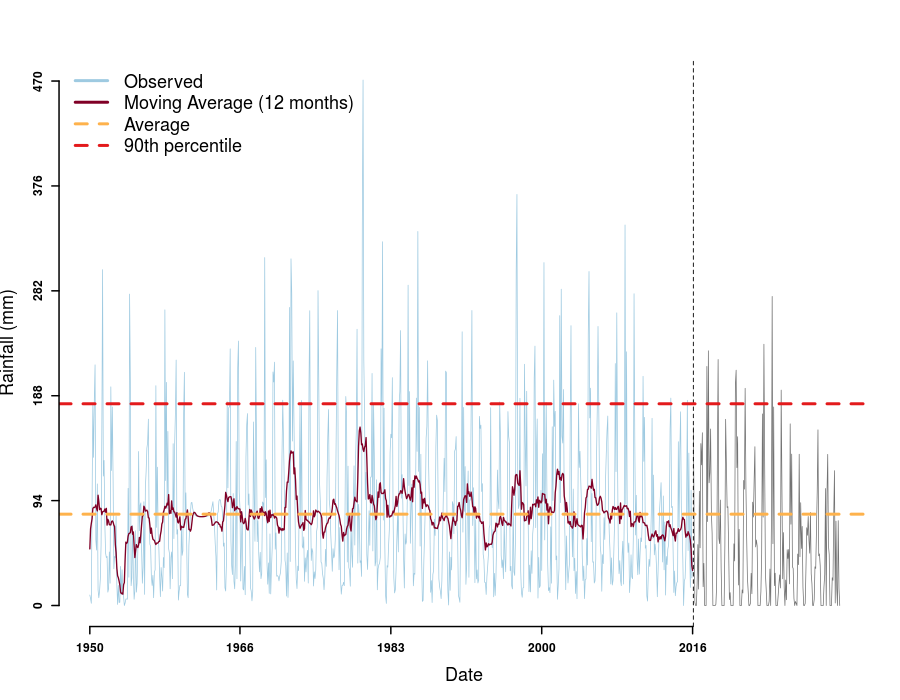
\includegraphics[width=.9\linewidth]{/home/demiurgo/Documents/PhD/Atlantis_Model/model_JFR/MandM/img/Rain_extreme.png}
\paragraph*{Constructing the ts per day}
\label{sec-5-3-1-3}

\begin{itemize}
\item I used the data of the peak day (days with more than 10mm per day) and the total day of rain to reconstruct the time seriw by days
\item I assume that the rain is distributed normal during the month
\end{itemize}

\begin{verbatim}
## Create the inputs files
## Average dischard form a small river is 516 MgNy-1
source('/home/demiurgo/Documents/PhD/Atlantis_Model/tools/Atlantis_tools.R')
Rivers <- read.csv('/home/demiurgo/Documents/PhD/Forcing_Files/NO3/Rivers.csv')
dat <- read.csv('/home/demiurgo/Documents/PhD/Forcing_Files/NO3/2-Rain_extrem.csv', sep = ' ')
month  <- c(31, 28, 31, 30, 31, 30, 31, 31, 30, 31, 30, 31)
peak   <- dat$peaks * 10
peak[is.na(peak)] <- 0
n.peak   <- dat$arima - peak
n.peak.d <- (dat$duration - dat$peaks)
ts       <- NULL
for(p in 1 : nrow(dat)){
    days <- month[dat$Month[p]]
    if(dat$Month[p] == 2 & dat$Year[p]%%4 == 0) days <- days + 1
    if(!is.na(dat$duration[p]) & n.peak[p] != 0){
        tmp.1 <- rep(n.peak[p] / n.peak.d[p], n.peak.d[p])
        tmp.2 <- rep(peak[p] / dat$peaks[p], dat$peaks[p])
        if(tmp.1[1] > 10){
            ## Keeping the same amoun of days below 10mm of rain
            tmp.1[] <- 9.9
            extra   <- n.peak[p] - sum(tmp.1)
            tmp.2 <- tmp.2[] + (extra / length(tmp.2))
        }
        tmp.3 <- c(tmp.1[1 : round(length(tmp.1) / 2)], tmp.2, tmp.1[(round(length(tmp.1) / 2) + 1) : length(tmp.1)] )
        left  <- days - length(tmp.3)
        tmp.4 <- c(rep(0, round(left / 2)), tmp.3, rep(0, (left - (round(left / 2)))))
    } else {
        tmp.4  <- rep(n.peak[p] / days, days)
    }
    final.1 <- data.frame(Year  = rep(dat$Year[p], days),
                          Month = rep(dat$Month[p], days),
                          Day   = 1 : days,
                          Rain  = tmp.4,
                          Peak  = rep(ifelse(is.na(dat$a.extreme[p]), FALSE, TRUE), days))
    ts <- rbind(ts, final.1)
}
ts$dates <- with(ts, as.Date(paste0(ts$Year,'/', ts$Month, '/', ts$Day), format = '%Y/%m/%d'))
ts$mean  <- movavg(ts$Rain, 15)
write.table(ts, file = '/home/demiurgo/Documents/PhD/Forcing_Files/NO3/3-daily_Rain.csv', row.names = FALSE)
by.year  <- tapply(dat$arima, dat$Year, sum)
years    <- 1950 : 2016
color    <- rgb(t(col2rgb("grey")), alpha = 250, maxColorValue = 255)
## plots
png('/home/demiurgo/Documents/PhD/Atlantis_Model/model_JFR/MandM/img/Rain.ts.png', width = 600, height = 900)
par(mfrow = c(3, 1), oma = c(3, 1, 1, 1), mar = c(2, 5, 1, 1))
## By Years
plot(years, unlist(by.year), yaxt = 'n', xaxt = 'n', bty = 'n',
     type = 'b', pch = 19,  xlab = 'Years', ylab = 'Rainfall per year (mm)')
tickx <- seq(from = 1950, to = 2016, length = 5)
yticks <- seq(0, max(by.year), by = round(max(by.year) / 5))
axis(2, at = yticks , labels = yticks, lwd = 2,  col = 1, las = 1)
axis(1, at = tickx, labels = tickx, lwd = 2,  col = 1)
## By month
plot(dat$arima, type = 'l', yaxt = 'n', xaxt = 'n', ylab = 'Rainfall per month (mm)', xlab = 'Date', bty = 'n')
tickx <- seq(from = 1, to = length(dat$date), length = 5)
yticks <- seq(0, max(dat$arima), by = round(max(dat$arima) / 5))
axis(2, at = yticks , labels = yticks, lwd = 2,  col = 1, las = 1)
axis(1, at = dat$date[tickx], labels = format.Date(dat$date[tickx], '%Y.%m'), lwd = 2,  col = 1)
## By day
plot(ts$Rain, type = 'l', yaxt = 'n', xaxt = 'n', ylab = 'Rainfall per day (mm)', xlab = 'Date', bty = 'n')
lines(ts$mean, col = 'firebrick')
tickx <- seq(from = 1, to = length(ts$dates), length = 5)
yticks <- seq(0, max(ts$Rain), by = round(max(ts$Rain) / 5))
axis(2, at = yticks , labels = yticks, lwd = 2,  col = 1, las = 1)
axis(1, at = tickx, labels = format.Date(ts$dates[tickx], '%Y.%m.%d'), lwd = 2,  col = 1)
dev.off()
\end{verbatim}
     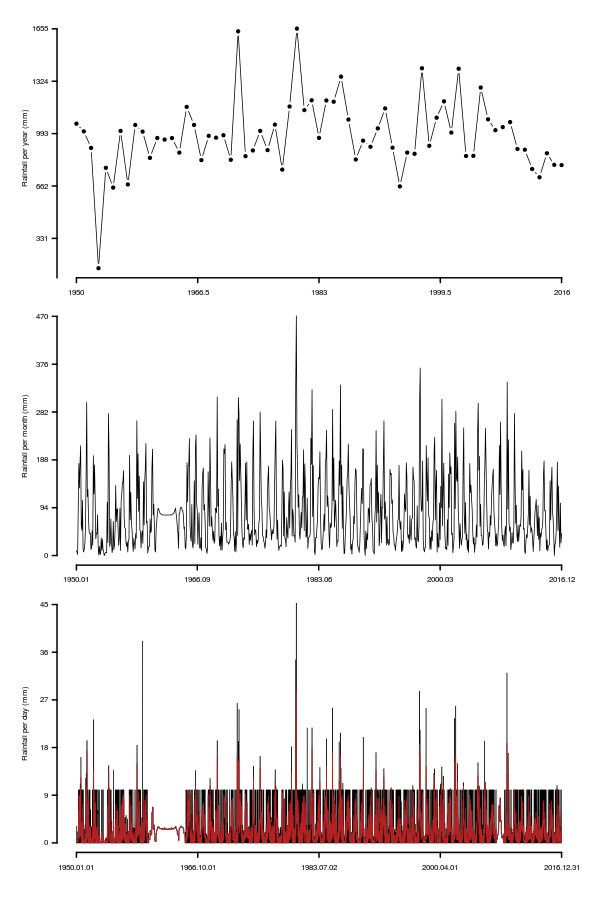
\includegraphics[width=.9\linewidth]{/home/demiurgo/Documents/PhD/Atlantis_Model/model_JFR/MandM/img/Rain.ts.png}
\paragraph*{Nitrogen}
\label{sec-5-3-1-4}

\begin{itemize}
\item to calculate the average amount of nitrogen in the river I used the relation of DIN=NO3+NO2+NH4. Assuming that in JF there is not to much waste I asummed that the total DIN is almost equal to NO3
\item from the database of Mayorga et al 2010 I use the average for the river of order 2 in the strahlet stream order of 157.4 KgNk2yr-1 (+-88.6)
\item The linear regresion equation was 0.0027316231 x River Area with an 0.72 of R2
\begin{itemize}
\item This gives a value of 0.08864117 DIN for Robisnon Asumming that 80\% of DIN is NO3 the todal NO3 is 0.0709129357 KgKm2y-1
\begin{itemize}
\item this would give a total of 2.302 Kgy-1
\item 2301124.7626862 NO3 Mgy-1
\end{itemize}
\end{itemize}
\end{itemize}

\begin{center}
\begin{tabular}{lr}
 River Area (Km2)  &  DIN (KgKm2y-1)  \\
\hline
 98,779            &           185.5  \\
 83,316            &           151.3  \\
 63,815            &           330.9  \\
 54,765            &           235.1  \\
 52,964            &            59.8  \\
 50,544            &            88.8  \\
 41,531            &           113.2  \\
 33,733            &           220.0  \\
 32,159            &            71.0  \\
 29,866            &            56.7  \\
 27,702            &           219.3  \\
\end{tabular}
\end{center}



\begin{itemize}
\item Las principales quebradas en Robisnon tienen un total de 32.45 km2
\end{itemize}
\subsection*{Initial conditions file}
\label{sec-5-4}

\begin{itemize}
\item To set the initial conditions I used the Shiny application and the code that create to fill the matrix of abundance and cover
\item The Shiny Application to create the csv files to fill

\begin{verbatim}
rm(list=ls())
source('/home/demiurgo/Documents/PhD/Atlantis_Model/tools/General_tools/Atlantis_tools.R')
## Using Shiny-R
library(stringr)
library(shiny)
library(dplyr)
library(shinyrAtlantis)
grp.file   <- "/home/demiurgo/Documents/PhD/Atlantis_Model/model_JFR/JFREGroups.csv"
bgm.file   <- "/home/demiurgo/Documents/PhD/Atlantis_Model/model_JFR/JFRE_xy.bgm"
cum.depths <- c(0, 20, 50, 150, 250, 400, 650, 1000, 4300)
csv.name   <- "JFRE_ini"
##~ Creation of the csv files
## i did some modification to the Shiny aplication, because of that I'm using my own code
source('/home/demiurgo/Documents/PhD/Atlantis_Model/tools/shiny-Shane/Fork_git/shinyrAtlantis/R/initGen.R')
make.init.csv(grp.file, bgm.file, cum.depths, csv.name)
\end{verbatim}
\item To complete the matrix created with shiny I used differente source of information:
\begin{itemize}
\item The initial total Abundance or biomass by group

\begin{center}
\begin{tabular}{lrrrl}
 FG   &  Mean Weight  &    Number  &           Biomass  &  reference                         \\
\hline
 SPL  &               &   1033572  &                    &  MPA Model                         \\
 GCR  &       697.06  &            &  327777.777777778  &  Canales y Arana 2009              \\
 BRC  &       754.93  &            &   2259.8263333333  &  Ernst 2016                        \\
 SPF  &       318.45  &            &   6927.6643333333  &  Ernst 2016                        \\
 SBF  &         1203  &            &    592.7413333333  &  Ernst 2016                        \\
 LBF  &      4125.24  &            &   1296.6216666667  &  Ernst 2016                        \\
 LPF  &         1000  &            &   1296.6216666667  &  Ernst 2016                        \\
 OCT  &          800  &            &           1110000  &  Arancibia                         \\
 BCA  &               &            &                    &  Friedlander2016                   \\
 VID  &         3755  &            &     37.0463333333  &  Ernst 2016                        \\
 SCR  &          618  &            &                    &  Friedlander2016 + Ernst Database  \\
 MOL  &               &            &                    &  Friedlander2016 + Ernst Database  \\
 ANG  &      1013.75  &            &                    &  Ernst Database                    \\
 ORO  &               &  36800000  &                    &  Niklitschek2005                   \\
 ALF  &               &  23222000  &                    &  Wiff et al. 2013                  \\
 CHO  &         4620  &            &                    &  Arana 2000 + Yañez                \\
 OTA  &        94000  &     31633  &                    &  Conaf and Osman 2007              \\
 CET  &     29215000  &     20128  &                    &  Estimation whale Watching         \\
 DOL  &       467500  &     40256  &                    &  Estimation whale Watching         \\
 BIR  &          740  &     19440  &                    &  Azocar 2013                       \\
 BFF  &               &            &                    &  Calculated from Friedlander2016   \\
 COR  &               &            &                    &  Calculated from Friedlander2016   \\
 MA   &               &            &                    &  Calculated from Friedlander2016   \\
 SQD  &               &            &           1110000  &  Same Value than Octopus           \\
\end{tabular}
\end{center}


\item The lenght or age distribution by cohort. I used the information calculated on \hyperref[sec-5-2-1-11]{Table}

\begin{verbatim}
## ~~~~~~~~~~~~~~~~~~~~~~~~~~~~~~~~~~~~~~~~~~~~~~ ##
## ~            Fill biomass and number         ~ ##
## ~~~~~~~~~~~~~~~~~~~~~~~~~~~~~~~~~~~~~~~~~~~~~~ ##
rm(list=ls())
library(ascii)
options(asciiType = "org")
source('/home/demiurgo/Documents/PhD/Atlantis_Model/tools/General_tools/Atlantis_tools.R')
##~ read proportion by box
filename <-'/home/demiurgo/Documents/PhD/Ini_conditions/PropByBox.csv'
grp.file <- "/home/demiurgo/Documents/PhD/Atlantis_Model/model_JFR/JFREGroups.csv"
data     <- read.csv(filename)
in.bios  <- read.csv('/home/demiurgo/Documents/PhD/Ini_conditions/In_abundance.csv')
boxes    <- read.poly('/home/demiurgo/Documents/PhD/Polygonos/Map/Polygons_27042016.csv')$attrib
groups   <- read.csv(grp.file)
lfd      <- read.csv('/home/demiurgo/Documents/PhD/Ini_conditions/Age_structure.csv')
cov.data <- read.csv('/home/demiurgo/Documents/PhD/Ini_conditions/Type.sed.csv')

BioNum <- init.number(data    = data, in.bios = in.bios,
                      boxes   = boxes, groups = groups, lfd = lfd, cover.d=cov.data)
#colnames(BioNum) <- paste('box', 0 : 50)
#cap <- 'number,biomass and percentage or cover by box'
#b   <- ascii(BioNum, header = T,  include.rownames = TRUE, include.colnames = TRUE, caption=cap, digits=3)
\end{verbatim}
\end{itemize}
\item Calculatin the Structural and reserve weight for each Functional Group

\begin{verbatim}
## ~~~~~~~~~~~~~~~~~~~~~~~~~~~~~~~~~~~~~~~~~~~~~~~~~~~ ##
## ~         Estimation of Nitrogen by Ageclass      ~ ##
## ~~~~~~~~~~~~~~~~~~~~~~~~~~~~~~~~~~~~~~~~~~~~~~~~~~~ ##
library(ascii)
library(ggplot2)
data  <- read.csv('/home/demiurgo/Documents/PhD/Functional_groups/Nitrogen_by_Agegroup/age_length.csv')
options(asciiType="org")
source('/home/demiurgo/Documents/PhD/Atlantis_Model/tools/General_tools/Atlantis_tools.R')
## estimation of the weight at each age class or cohort
data$Weight     <- ifelse(is.na(data$Weight), alometric(data$Length, data$alfa, data$beta), data$Weight)
w.data     <- with(data, weights(FG, Weight, 'g', wet = TRUE))
w.data$AgeClass <- data$AgeClass
## Plotting
sp            <- ggplot(data = w.data, aes(AgeClass, label = 'Weight')) +
    geom_line(aes(y = reserve, colour = 'Reserve')) +
    geom_line(aes(y = structural, colour = 'Structural')) +
    xlab("Cohort") +
    ylab("Weight (MgN)")
png('img/rev_stru.png', height = 1200, width = 1200)
sp + facet_wrap(~Functional_Groups, ncol=4, scales = 'free')
invisible(dev.off())
## Table
tab.out <- xtabs(cbind(reserve, structural) ~ Functional_Groups + AgeClass, w.data)
cap1    <- 'Reserve by cohort for each functional group [mgN]'
cap2    <- 'Structural by cohort for each functional group [mgN]'
b       <- ascii(tab.out[, , 1], header=T,  include.rownames = TRUE, include.colnames = T, caption = cap1)
c       <- ascii(tab.out[, , 2], header=T,  include.rownames = TRUE, include.colnames = T, caption = cap2)
cat("#+ATTR_HTML: :style float:left;width:30%;margin:3ex\n")
print(b)
print(c)
\end{verbatim}
\end{itemize}
\begin{table}[htb]
\caption{Reserve by cohort for each functional group [mgN]}
\begin{center}
\begin{tabular}{llrrrrrrrrrr}
                             &       &  \textbf{AgeClass}  &                &                &                &                &                &                &                &                &                \\
                             &       &                  1  &             2  &             3  &             4  &             5  &             6  &             7  &             8  &             9  &            10  \\
\hline
 \textbf{Functional_Groups}  &  ALF  &            1114.87  &       2948.43  &       5396.66  &       8185.49  &      11084.29  &      13926.20  &      16607.07  &      19061.17  &      21273.52  &      23214.61  \\
                             &  ANG  &               5.14  &        476.77  &       2073.97  &       4803.25  &       8410.48  &      12585.66  &      17045.88  &      21564.06  &      25973.03  &      30159.05  \\
                             &  BIR  &              69.13  &        415.90  &       1066.08  &       1938.17  &       2931.67  &       3960.82  &       4963.61  &       5900.56  &       6750.08  &       7503.41  \\
                             &  BRC  &             681.99  &       1187.86  &       1903.52  &       2835.69  &       4071.67  &       5794.55  &       7999.09  &      10088.06  &      12271.21  &      14756.34  \\
                             &  CET  &       395155425.63  &  491609711.65  &  544190946.98  &  571307526.53  &  584935787.29  &  591701186.84  &  595039702.45  &  596682367.21  &  597489464.60  &  597885742.56  \\
                             &  CHO  &             463.86  &       2929.85  &       7534.30  &      13527.87  &      20078.00  &      26550.51  &      32550.19  &      37876.85  &      42464.82  &      46330.94  \\
                             &  DOL  &            4307.42  &      25566.65  &      64722.96  &     116326.38  &     174114.22  &     232990.31  &     289446.06  &     341384.57  &     387777.19  &     428327.01  \\
                             &  GCR  &              34.97  &        192.81  &        549.34  &       1157.33  &       2026.08  &       3072.45  &       4122.86  &       5046.51  &       6094.64  &       7068.33  \\
                             &  LBF  &            6768.28  &      10195.69  &      15630.74  &      20771.14  &      27974.29  &      41908.11  &      55595.37  &      65347.40  &      81692.38  &     101344.52  \\
                             &  LPF  &             404.38  &       5842.40  &      12058.50  &      16171.97  &      18457.96  &      19640.82  &      20233.53  &      20526.09  &      20669.46  &      20739.47  \\
                             &  ORO  &              22.09  &       2272.61  &       6693.94  &      10880.49  &      14018.78  &      16142.69  &      17503.25  &      18351.23  &      18864.25  &      19174.35  \\
                             &  OTA  &          201231.61  &     305483.96  &     393956.61  &     463082.98  &     514521.02  &     551653.23  &     577941.71  &     596317.57  &     609054.39  &     617832.86  \\
                             &  SBF  &            2378.48  &       3132.71  &       3940.00  &       5003.55  &       6092.65  &       7518.46  &       8371.08  &      10308.91  &      11475.56  &      12675.33  \\
                             &  SPF  &              16.46  &        530.71  &       1768.56  &       3321.01  &       4832.29  &       6127.44  &       7159.38  &       7945.64  &       8527.77  &       8950.70  \\
                             &  SPL  &             120.03  &       1663.26  &       4319.65  &       7481.69  &      10641.26  &      13514.84  &      15983.59  &      18027.49  &      19677.74  &      27378.12  \\
                             &  VID  &           10104.27  &      15617.54  &      24989.94  &          0.00  &          0.00  &          0.00  &          0.00  &          0.00  &          0.00  &          0.00  \\
                             &       &  \textbf{AgeClass}  &                &                &                &                &                &                &                &                &                \\
                             &       &                  1  &             2  &             3  &             4  &             5  &             6  &             7  &             8  &             9  &            10  \\
\hline
 \textbf{Functional_Groups}  &  ALF  &             420.71  &       1112.62  &       2036.47  &       3088.86  &       4182.75  &       5255.17  &       6266.82  &       7192.89  &       8027.74  &       8760.23  \\
                             &  ANG  &               1.94  &        179.91  &        782.63  &       1812.55  &       3173.77  &       4749.31  &       6432.41  &       8137.38  &       9801.14  &      11380.77  \\
                             &  BIR  &              26.09  &        156.94  &        402.29  &        731.39  &       1106.29  &       1494.65  &       1873.06  &       2226.63  &       2547.20  &       2831.48  \\
                             &  BRC  &             257.35  &        448.25  &        718.31  &       1070.07  &       1536.48  &       2186.62  &       3018.53  &       3806.81  &       4630.64  &       5568.43  \\
                             &  CET  &       149115254.95  &  185513098.74  &  205355074.33  &  215587745.86  &  220730485.77  &  223283466.73  &  224543283.94  &  225163157.44  &  225467722.49  &  225617261.34  \\
                             &  CHO  &             175.04  &       1105.61  &       2843.13  &       5104.86  &       7576.61  &      10019.06  &      12283.09  &      14293.15  &      16024.46  &      17483.37  \\
                             &  DOL  &            1625.44  &       9647.79  &      24423.76  &      43896.75  &      65703.48  &      87920.87  &     109224.93  &     128824.36  &     146331.01  &     161632.83  \\
                             &  GCR  &              13.20  &         72.76  &        207.30  &        436.73  &        764.56  &       1159.42  &       1555.79  &       1904.34  &       2299.86  &       2667.29  \\
                             &  LBF  &            2554.07  &       3847.43  &       5898.39  &       7838.17  &      10556.34  &      15814.38  &      20979.38  &      24659.40  &      30827.31  &      38243.22  \\
                             &  LPF  &             152.60  &       2204.68  &       4550.38  &       6102.63  &       6965.27  &       7411.63  &       7635.29  &       7745.69  &       7799.80  &       7826.22  \\
                             &  ORO  &               8.33  &        857.59  &       2526.02  &       4105.85  &       5290.11  &       6091.58  &       6605.00  &       6924.99  &       7118.59  &       7235.60  \\
                             &  OTA  &           75936.46  &     115276.97  &     148662.87  &     174748.30  &     194158.88  &     208171.03  &     218091.21  &     225025.50  &     229831.84  &     233144.47  \\
                             &  SBF  &             897.54  &       1182.16  &       1486.79  &       1888.13  &       2299.11  &       2837.16  &       3158.90  &       3890.16  &       4330.40  &       4783.14  \\
                             &  SPF  &               6.21  &        200.27  &        667.38  &       1253.21  &       1823.51  &       2312.24  &       2701.65  &       2998.36  &       3218.03  &       3377.62  \\
                             &  SPL  &              45.29  &        627.64  &       1630.06  &       2823.28  &       4015.57  &       5099.94  &       6031.54  &       6802.83  &       7425.56  &      10331.37  \\
                             &  VID  &            3812.93  &       5893.41  &       9430.17  &          0.00  &          0.00  &          0.00  &          0.00  &          0.00  &          0.00  &          0.00  \\
\end{tabular}
\end{center}
\end{table}

   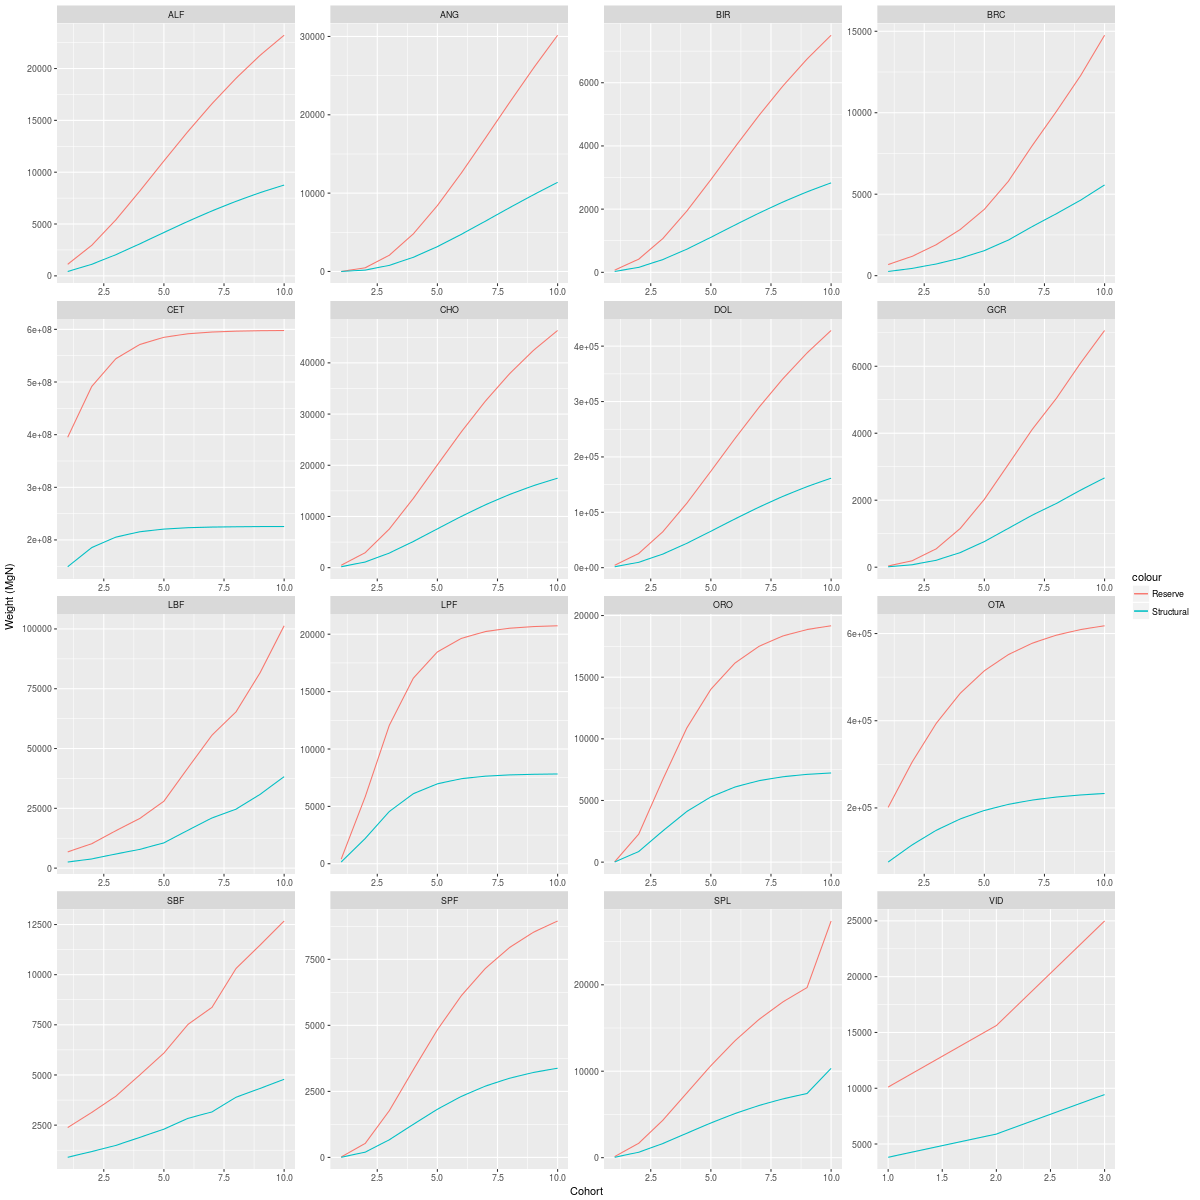
\includegraphics[width=.9\linewidth]{/home/demiurgo/Documents/PhD/Atlantis_Model/model_JFR/MandM/img/rev_stru.png}
\begin{itemize}
\item Write the csv and the nc file witht he information

\begin{verbatim}
## ~~~~~~~~~~~~~~~~~~~~~~~~~~~~~~~~~~~~~~~~~~~~~~~~~~~~~~~~~~~~~~~~ ##
## ~                 Write the information on the CSV             ~ ##
## ~~~~~~~~~~~~~~~~~~~~~~~~~~~~~~~~~~~~~~~~~~~~~~~~~~~~~~~~~~~~~~~~ ##
## Library and Sources
source('/home/demiurgo/Documents/PhD/Atlantis_Model/tools/General_tools/Atlantis_tools.R')
## read Shiny File
shy.file <- '/home/demiurgo/Documents/PhD/Ini_conditions/JFRE_ini_horiz.csv'
csv.file <- read.csv(shy.file)
## Read the data file
dat.file <- '/home/demiurgo/Documents/PhD/Ini_conditions/Initial.Abundance.csv'
csv.dat  <- read.table(dat.file, sep=' ', row.names = 1)
i = 1
for(i in 1 : nrow(csv.dat)){
    ## modified the currrent values
    pos.csv <- which(csv.file$Variable %in% rownames(csv.dat)[i])
    csv.file[pos.csv, 2 : ncol(csv.file)] <- as.numeric(csv.dat[i, ])
}
write.table(csv.file, file = '/home/demiurgo/Documents/PhD/Ini_conditions/JFRE_ini_horiz.csv', row.names = FALSE)

## ~~~~~~~~~~~~~~~~~~~~~~~~~~~~~~~~~~~~~~~~~~~~~~ ##
## ~            Creation of the nc file         ~ ##
## ~~~~~~~~~~~~~~~~~~~~~~~~~~~~~~~~~~~~~~~~~~~~~~ ##
library(shinyrAtlantis)
library(ncdf4)
grp.file    <- "/home/demiurgo/Documents/PhD/Atlantis_Model/model_JFR/JFREGroups.csv"
bgm.file    <- "/home/demiurgo/Documents/PhD/Atlantis_Model/model_JFR/JFRE_xy.bgm"
JFRE.init   <- "/home/demiurgo/Documents/PhD/Ini_conditions/JFRE_ini_init.csv"
JFRE.init.h <- "/home/demiurgo/Documents/PhD/Ini_conditions/JFRE_ini_horiz.csv"
cum.depths  <- c(0, 20, 50, 150, 250, 400, 650, 1000, 4300)
nc.file     <- "/home/demiurgo/Documents/PhD/Ini_conditions/JFRE.ini.nc"
make.init.nc(bgm.file, cum.depths, JFRE.init, JFRE.init.h, nc.file)
\end{verbatim}
\end{itemize}
\subsubsection*{Burning period}
\label{sec-6-1}

\begin{itemize}
\item The burning period that was setted for the model was 31 years. During this time most
  of the functional groups reached and stable age distribution.
\end{itemize}
\paragraph*{General Changes}
\label{sec-6-1-1}

\begin{itemize}
\item Days 11306 for the burning period (almos 31 years)
\item All the Forcing files were replicated 31 years for the bigining of the
  simulation.  I repeated the infomation for :
\begin{itemize}
\item Recruitment Conectivity
\begin{itemize}
\item Increased historical values

\begin{verbatim}
## Use nco to concatenate the files, is easy and fast
## file with repeating the 31 first years
ncks -d t,0,30 FG_connect.nc Burn.nc
## append the initial values to the file
ncrcat -h Burn.nc FG_connect.nc FG_connect_Burn.nc
\end{verbatim}
\end{itemize}
\item Hidrodaynamic : Fluxes of nutrients, temperature and salinity
\item Eddies by box
\item Solar radiation
\end{itemize}
\end{itemize}
\paragraph*{Fisheries}
\label{sec-6-1-2}

\begin{itemize}
\item In the JFRE all the artisanal fisheries start almost in 1900 except GCR. To
   represent this I start the model under an exploitation state. I start all the
   fisheries 6 years before the start of the model,  that provides and age
   distribution very similar to the one reported in the JFRE MPA model
\end{itemize}
\subsubsection*{Projections}
\label{sec-6-2}

\begin{itemize}
\item I use the CMPI5 scenarios
\end{itemize}
Future   projections   (2006-2100) forced by RCP 2.6 and 8.5. RCP
s (representative concentration pathways) approximately result in radiative forcings of 2.6, 4.5, 6.0 and 8.5 W m
-2 at  year 2100 respectively, relative to pre-industrial conditions.
\begin{itemize}
\item RCP-2.6
\item RCP-8.5
\item The model that I used was the output from the GDFL (\href{http://nomads.gfdl.noaa.gov:8080/DataPortal/cmip5.jsp}{http://nomads.gfdl.noaa.gov:8080/DataPortal/cmip5.jsp}).
\begin{itemize}
\item Using the model
       ESM2M, pressure-based vertical coordinates are used along the developmental path of
\item Getting the Data

\begin{verbatim}
ncks -d rlon,194,210  -d rlat,41,53 http://nomads.gfdl.noaa.gov/dods-data/CMIP5/output1/NOAA-GFDL/GFDL-ESM2M/rcp85/mon/ocean/Omon/r1i1p1/v20110601/thetao/thetao_Omon_GFDL-ESM2M_rcp85_r1i1p1_201101-201512.nc -o Proj_2011.nc
ncks -d rlon,194,210  -d rlat,41,53 http://nomads.gfdl.noaa.gov/dods-data/CMIP5/output1/NOAA-GFDL/GFDL-ESM2M/rcp85/mon/ocean/Omon/r1i1p1/v20110601/thetao/thetao_Omon_GFDL-ESM2M_rcp85_r1i1p1_201601-202012.nc -o Proj_2016.nc
ncks -d rlon,194,210  -d rlat,41,53 http://nomads.gfdl.noaa.gov/dods-data/CMIP5/output1/NOAA-GFDL/GFDL-ESM2M/rcp85/mon/ocean/Omon/r1i1p1/v20110601/thetao/thetao_Omon_GFDL-ESM2M_rcp85_r1i1p1_202101-202512.nc -o Proj_2021.nc
ncks -d rlon,194,210  -d rlat,41,53 http://nomads.gfdl.noaa.gov/dods-data/CMIP5/output1/NOAA-GFDL/GFDL-ESM2M/rcp85/mon/ocean/Omon/r1i1p1/v20110601/thetao/thetao_Omon_GFDL-ESM2M_rcp85_r1i1p1_202601-203012.nc -o Proj_2026.nc
ncks -d rlon,194,210  -d rlat,41,53 http://nomads.gfdl.noaa.gov/dods-data/CMIP5/output1/NOAA-GFDL/GFDL-ESM2M/rcp85/mon/ocean/Omon/r1i1p1/v20110601/thetao/thetao_Omon_GFDL-ESM2M_rcp85_r1i1p1_203101-203512.nc -o Proj_2031.nc
ncks -d rlon,194,210  -d rlat,41,53 http://nomads.gfdl.noaa.gov/dods-data/CMIP5/output1/NOAA-GFDL/GFDL-ESM2M/rcp85/mon/ocean/Omon/r1i1p1/v20110601/thetao/thetao_Omon_GFDL-ESM2M_rcp85_r1i1p1_203601-204012.nc -o Proj_2036.nc
ncks -d rlon,194,210  -d rlat,41,53 http://nomads.gfdl.noaa.gov/dods-data/CMIP5/output1/NOAA-GFDL/GFDL-ESM2M/rcp85/mon/ocean/Omon/r1i1p1/v20110601/thetao/thetao_Omon_GFDL-ESM2M_rcp85_r1i1p1_204101-204512.nc -o Proj_2041.nc
ncks -d rlon,194,210  -d rlat,41,53 http://nomads.gfdl.noaa.gov/dods-data/CMIP5/output1/NOAA-GFDL/GFDL-ESM2M/rcp85/mon/ocean/Omon/r1i1p1/v20110601/thetao/thetao_Omon_GFDL-ESM2M_rcp85_r1i1p1_204601-205012.nc -o Proj_2046.nc
ncks -d rlon,194,210  -d rlat,41,53 http://nomads.gfdl.noaa.gov/dods-data/CMIP5/output1/NOAA-GFDL/GFDL-ESM2M/rcp85/mon/ocean/Omon/r1i1p1/v20110601/thetao/thetao_Omon_GFDL-ESM2M_rcp85_r1i1p1_205101-205512.nc -o Proj_2051.nc
ncks -d rlon,194,210  -d rlat,41,53 http://nomads.gfdl.noaa.gov/dods-data/CMIP5/output1/NOAA-GFDL/GFDL-ESM2M/rcp85/mon/ocean/Omon/r1i1p1/v20110601/thetao/thetao_Omon_GFDL-ESM2M_rcp85_r1i1p1_205601-206012.nc -o Proj_2056.nc
ncks -d rlon,194,210  -d rlat,41,53 http://nomads.gfdl.noaa.gov/dods-data/CMIP5/output1/NOAA-GFDL/GFDL-ESM2M/rcp85/mon/ocean/Omon/r1i1p1/v20110601/thetao/thetao_Omon_GFDL-ESM2M_rcp85_r1i1p1_206101-206512.nc -o Proj_2061.nc
ncks -d rlon,194,210  -d rlat,41,53 http://nomads.gfdl.noaa.gov/dods-data/CMIP5/output1/NOAA-GFDL/GFDL-ESM2M/rcp85/mon/ocean/Omon/r1i1p1/v20110601/thetao/thetao_Omon_GFDL-ESM2M_rcp85_r1i1p1_206601-207012.nc -o Proj_2066.nc
ncks -d rlon,194,210  -d rlat,41,53 http://nomads.gfdl.noaa.gov/dods-data/CMIP5/output1/NOAA-GFDL/GFDL-ESM2M/rcp85/mon/ocean/Omon/r1i1p1/v20110601/thetao/thetao_Omon_GFDL-ESM2M_rcp85_r1i1p1_207101-207512.nc -o Proj_2071.nc
ncks -d rlon,194,210  -d rlat,41,53 http://nomads.gfdl.noaa.gov/dods-data/CMIP5/output1/NOAA-GFDL/GFDL-ESM2M/rcp85/mon/ocean/Omon/r1i1p1/v20110601/thetao/thetao_Omon_GFDL-ESM2M_rcp85_r1i1p1_207601-208012.nc -o Proj_2076.nc
ncks -d rlon,194,210  -d rlat,41,53 http://nomads.gfdl.noaa.gov/dods-data/CMIP5/output1/NOAA-GFDL/GFDL-ESM2M/rcp85/mon/ocean/Omon/r1i1p1/v20110601/thetao/thetao_Omon_GFDL-ESM2M_rcp85_r1i1p1_208101-208512.nc -o Proj_2081.nc
ncks -d rlon,194,210  -d rlat,41,53 http://nomads.gfdl.noaa.gov/dods-data/CMIP5/output1/NOAA-GFDL/GFDL-ESM2M/rcp85/mon/ocean/Omon/r1i1p1/v20110601/thetao/thetao_Omon_GFDL-ESM2M_rcp85_r1i1p1_208601-209012.nc -o Proj_2086.nc
ncks -d rlon,194,210  -d rlat,41,53 http://nomads.gfdl.noaa.gov/dods-data/CMIP5/output1/NOAA-GFDL/GFDL-ESM2M/rcp85/mon/ocean/Omon/r1i1p1/v20110601/thetao/thetao_Omon_GFDL-ESM2M_rcp85_r1i1p1_209101-209512.nc -o Proj_2091.nc
ncks -d rlon,194,210  -d rlat,41,53 http://nomads.gfdl.noaa.gov/dods-data/CMIP5/output1/NOAA-GFDL/GFDL-ESM2M/rcp85/mon/ocean/Omon/r1i1p1/v20110601/thetao/thetao_Omon_GFDL-ESM2M_rcp85_r1i1p1_209601-210012.nc -o Proj_2096.nc
\end{verbatim}
\end{itemize}
\end{itemize}
\paragraph*{Recruitment deviation}
\label{sec-6-2-1}

\begin{itemize}
\item For the projection of the recruitmen deviation of lobster used an arima model
\begin{itemize}
\item I add the noise to the arima,  the noise was calculate from the same observed deviation
\end{itemize}
\end{itemize}

\begin{verbatim}
## Creating the files and the time series
source('/home/demiurgo/Documents/PhD/Atlantis_Model/tools/General_tools/Atlantis_tools.R')
library('forecast')
## Average dischard form a small river is 516 MgNy-1
## reading data
dat    <- read.csv('/home/demiurgo/Documents/PhD/Forcing_Files/Recruitmen/SPL/rec.csv')
new    <- exp(dat[,2]) #movavg(exp(dat[,2]), 10) #/ mean(movavg(exp(dat[,2]), 10))
#new    <-  new-min(new)
new       <- rep(new, each = 365)
time      <- seq(from = 1, by = 1, length = length(new))
var.name  <- 'SPL'
long.name <- 'SPL'
units     <- 'scalar'
time.unit = 'days since 1900-01-01 00:00:0.0'
#debug(write.ts)

data <- cbind(time, new)
write.ts(var.name, ext.nam = '_rec_dev', dat = data, long.name, units, time.unit)
##Projection of recruitment
## I use an arima model to wet the seasonal variation
## I use the remove the noise from the signal and I added to the projected values
g.rec <- movavg(dat[1 : (nrow(dat) - 5), 2], 5)
lpass <- smooth.spline(x=c(1 : 111), y = g.rec) ## Control spar for amount of smoothing
noise <- g.rec-predict(lpass, x = c(1 : 111))$y
fit   <- auto.arima(g.rec, stepwise = FALSE, approximation = FALSE)
set.seed(100)
n.sim <- rnorm(40, mean = mean(noise), sd = sd(noise))
mean  <- as.vector(forecast(fit, 40)$mean) + n.sim
low   <- as.vector(forecast(fit, 40)$lower[, 2]) + n.sim # 95% confidence
upper <- as.vector(forecast(fit, 40)$upper[, 2]) + n.sim # 95% confidence
mean  <- rep(c(dat[1 : (nrow(dat) - 5), 2], mean), each = 365)
low   <- rep(c(dat[1 : (nrow(dat) - 5), 2], low), each = 365)
upper <- rep(c(dat[1 : (nrow(dat) - 5), 2], upper), each = 365)
time.proj <- seq(from = 1, by = 1, length = length(mean))
mean.proj <- cbind(time.proj, mean)
low.proj  <- cbind(time.proj, low)
upp.proj  <- cbind(time.proj, upper)

write.ts(var.name, ext.nam = '_Good_rec_dev', dat = mean.proj, long.name, units, time.unit)
write.ts(var.name, ext.nam = '_BAD_rec_dev', dat = low.proj, long.name, units, time.unit)
write.ts(var.name, ext.nam = '_MEAN_grec_dev', dat = upp.proj, long.name, units, time.unit)
\end{verbatim}
\paragraph*{Fishing scenarios}
\label{sec-6-2-2}

\begin{itemize}
\item I calculate the percentage on change respect to the initial value
\item The day of change including the burning period is 35048 days (1919-01-17 to 2015-01-01)
\end{itemize}


\begin{center}
\begin{tabular}{llrrrrrrrrr}
              &       &        Fvalues  &                         &                         &                         &                         &                         &                         &                         &                         \\
\hline
              &       &  Initial value  &     Last value Indcast  &                    BAU  &              ICRUS20\%  &              ICRUS50\%  &                  IBOTH  &             IFISH.20\%  &             IFISH.50\%  &            IFISH.100\%  \\
\hline
 Crustaceans  &  SPL  &   0.0002248651  &           0.0021982979  &           0.0021982979  &           0.0026379575  &           0.0032974469  &           0.0026379575  &           0.0021982979  &           0.0021982979  &           0.0021982979  \\
              &  GCR  &      0.0001370  &           0.0013390964  &           0.0013390964  &           0.0016069157  &           0.0020086447  &           0.0016069157  &           0.0013390964  &           0.0013390964  &           0.0013390964  \\
              &  ANG  &      0.0000052  &  5.09374233768119E-005  &  5.09374233768119E-005  &  6.11249080521743E-005  &  7.64061350652178E-005  &  6.11249080521743E-005  &  5.09374233768119E-005  &  5.09374233768119E-005  &  5.09374233768119E-005  \\
              &  BRC  &      0.0000059  &  5.80942727020646E-005  &  5.80942727020646E-005  &  6.97131272424776E-005  &   8.7141409053097E-005  &  6.97131272424776E-005  &  5.80942727020646E-005  &  5.80942727020646E-005  &  5.80942727020646E-005  \\
              &  LBF  &      0.0000002  &            0.000001981  &            0.000001981  &  2.37717789018062E-006  &  2.97147236272578E-006  &  4.75435578036124E-006  &  2.37717789018062E-006  &  2.97147236272578E-006  &            0.000003962  \\
              &  LPF  &      0.0000043  &  4.23891525526004E-005  &  4.23891525526004E-005  &            0.000050867  &  6.35837288289007E-005  &            0.000101734  &            0.000050867  &  6.35837288289007E-005  &  8.47783051052009E-005  \\
              &  SBF  &      0.0000001  &   1.3373042468961E-006  &   1.3373042468961E-006  &  1.60476509627532E-006  &            0.000002006  &  3.20953019255064E-006  &  1.60476509627532E-006  &            0.000002006  &   2.6746084937922E-006  \\
              &  SPF  &      0.0000004  &  3.96768970141835E-006  &  3.96768970141835E-006  &  4.76122764170201E-006  &  5.95153455212752E-006  &  9.52245528340403E-006  &  4.76122764170201E-006  &  5.95153455212752E-006  &  7.93537940283669E-006  \\
\hline
 Finfish      &  BRC  &      0.0000047  &  4.74153232332686E-006  &  4.74153232332686E-006  &  4.74153232332686E-006  &  4.74153232332686E-006  &  5.68983878799223E-006  &  5.68983878799223E-006  &  7.11229848499029E-006  &  9.48306464665372E-006  \\
              &  VID  &      0.0000010  &   9.8076897048216E-007  &   9.8076897048216E-007  &   9.8076897048216E-007  &   9.8076897048216E-007  &  1.17692276457859E-006  &  1.17692276457859E-006  &  1.47115345572324E-006  &  1.96153794096432E-006  \\
              &  OCT  &      0.0000693  &  6.93063561749696E-005  &  6.93063561749696E-005  &  6.93063561749696E-005  &  6.93063561749696E-005  &  8.31676274099635E-005  &  8.31676274099635E-005  &           0.0001039595  &           0.0001386127  \\
\end{tabular}
\end{center}




\begin{itemize}
\item Percentage of Change
\end{itemize}

\begin{center}
\begin{tabular}{llrrrrrrr}
              &  Fishery   &      BAU  &  ICRUS20\%  &  ICRUS50\%  &     IBOTH  &  IFISH.20\%  &  IFISH.50\%  &  IFISH.100\%  \\
\hline
 Crustaceans  &  TrapSPL   &  9.77607  &   11.73129  &   14.66411  &  11.73129  &     9.77607  &     9.77607  &      9.77607  \\
              &  TrapGCR   &  9.77607  &   11.73129  &   14.66411  &  11.73129  &     9.77607  &     9.77607  &      9.77607  \\
              &  TrapANG   &  9.77607  &   11.73129  &   14.66411  &  11.73129  &     9.77607  &     9.77607  &      9.77607  \\
              &  BaitBRC   &  9.77607  &   11.73129  &   14.66411  &  11.73129  &     9.77607  &     9.77607  &      9.77607  \\
              &  BaitLBF   &  9.77607  &   11.73129  &   14.66411  &  23.46258  &    11.73129  &    14.66411  &     19.55215  \\
              &  BaitLPF   &  9.77607  &   11.73129  &   14.66411  &  23.46258  &    11.73129  &    14.66411  &     19.55215  \\
              &  BaitSBF   &  9.77607  &   11.73129  &   14.66411  &  23.46258  &    11.73129  &    14.66411  &     19.55215  \\
              &  BaitSPF   &  9.77607  &   11.73129  &   14.66411  &  23.46258  &    11.73129  &    14.66411  &     19.55215  \\
\hline
 Finfish      &  HlineBRC  &  1.00000  &    1.00000  &    1.00000  &   1.20000  &     1.20000  &     1.50000  &      2.00000  \\
              &  HlineVID  &  1.00000  &    1.00000  &    1.00000  &   1.20000  &     1.20000  &     1.50000  &      2.00000  \\
              &  PotOCT    &  1.00000  &    1.00000  &    1.00000  &   1.20000  &     1.20000  &     1.50000  &      2.00000  \\
\end{tabular}
\end{center}
\subsubsection*{Sensitivity Analsisys}
\label{sec-6-3}

\begin{itemize}
\item I tested the initial biomass for several groups, for those that I did't have a clear estimation
\item Scenarios :
\end{itemize}

\begin{center}
\begin{tabular}{llrrrrrr}
 FG   &  Scenario  &  BRC  &  ANG  &  LPF  &  SPF  &  SBF  &  LBF  \\
\hline
 ANG  &  UP        &    1  &  1.5  &    1  &    1  &  0.8  &    1  \\
      &  DOWN      &    1  &  0.5  &    1  &    1  &  0.8  &    1  \\
\hline
 BRC  &  UP        &  1.5  &    1  &    1  &    1  &  0.8  &    1  \\
      &  DOWN      &  0.5  &    1  &    1  &    1  &  0.8  &    1  \\
\hline
 LBF  &  UP        &    1  &    1  &    1  &    1  &  0.8  &  1.5  \\
      &  DOWN      &    1  &    1  &    1  &    1  &  0.8  &  0.5  \\
\hline
 LPF  &  UP        &    1  &    1  &  1.5  &    1  &  0.8  &    1  \\
      &  DOWN      &    1  &    1  &  0.5  &    1  &  0.8  &    1  \\
\hline
 SBF  &  UP        &    1  &    1  &    1  &    1  &  1.2  &    1  \\
      &  DOWN      &    1  &    1  &    1  &    1  &  0.4  &    1  \\
\hline
 SPF  &  UP        &    1  &    1  &    1  &  1.5  &  0.8  &    1  \\
      &  DOWN      &    1  &    1  &    1  &  0.5  &  0.8  &    1  \\
\end{tabular}
\end{center}
\section*{Running Atlantis}
\label{sec-6}
\section*{Dietary analysis (DNA)}
\label{sec-7}
\subsection*{NGS}
\label{sec-7-1}

      I will use NGS for the analysis of the dietary relationship between the functional groups
\subsubsection*{Procedure}
\label{sec-7-1-1}

\begin{itemize}
\item DNA-extraccion
\begin{itemize}
\item Feacal extraction kit
\begin{itemize}
\item PowerFecal DNA Isolation Kit code : MB-12830-50
       Price : \$439.00 ex. GST. kit of 50
\end{itemize}
\end{itemize}
\item Concentration determination
\begin{itemize}
\item Fluorecense at UTAS
\end{itemize}
\item Amplicon PCR
\begin{itemize}
\item Tailed primers  + 10\% untailed primers
\begin{itemize}
\item Primers
\begin{itemize}
\item Furseal
\item Lobster
\item Fish
\end{itemize}
\end{itemize}
\item Taq polymerase
\item ddH2O
\end{itemize}
\item Clean Up
\item Gel
   To check if PCR works
\item Index PCR
\begin{itemize}
\item Nextera index kit
\item Kapa mix
\item ddH2O
\end{itemize}
\item Checking PCR
\item Quantify amount of DNA
\begin{itemize}
\item Quantiflour kit
\end{itemize}
\item Normalize the samples
\item Pool all the samples
\item Sequence in illumina MiSeq
\begin{itemize}
\item Sequencing reagents (1500 for ??)
\end{itemize}
\end{itemize}
\subsubsection*{Results}
\label{sec-7-1-2}

\begin{itemize}
\item DNA-extraction
\end{itemize}

\begin{center}
\begin{tabular}{rllll}
 ID  &  Specie           &  JF-ID   &     &     \\
\hline
  1  &  Pulpo            &  Pu_23   &     &     \\
  2  &  cangrejo dorado  &  CD_10   &     &     \\
  3  &  Lobo de mar      &  Lb_28   &     &     \\
  4  &  Breca            &  Bre_21  &     &     \\
  5  &  Vidriola         &  Vi_25   &     &     \\
  6  &  Vidriola         &  Vi_13   &     &     \\
  7  &  Chancharro       &  Ch_6    &     &     \\
  8  &  Jurelillo        &  Jur_9   &     &     \\
  9  &  Pez payaso?      &  P_7     &     &     \\
 10  &  Vidriola         &  Vi_18   &     &     \\
 11  &  Breca            &  Bre_14  &     &     \\
 12  &  Breca            &  Bre_5   &     &     \\
 13  &  Vidriola         &  Vi_26   &     &     \\
 14  &  Vidriola         &  Vi_22   &     &     \\
 15  &  Breca            &  Bre_16  &     &     \\
 16  &  jurel            &  Ju_15   &     &     \\
 17  &  Lobo de mar      &  Lb_27   &     &     \\
 18  &  Vidriola         &  Vi_17   &     &     \\
 19  &  Vidriola         &  Vi_20   &     &     \\
 20  &  Breca            &  Bre_24  &     &     \\
 21  &  Breca            &  Bre_19  &     &     \\
\end{tabular}
\end{center}
\subsection*{Cost DNA procedure}
\label{sec-7-2}

-All the cost are in AUD

\begin{center}
\begin{tabular}{lrlrr}
 Step-materials       &  Total Amount  &  Price unit           &  Total Price (182)  &  Total (96)  \\
\hline
 Consumables          &           Lot  &  300                  &                300  &         300  \\
 DNA-Extraccion       &            96  &  439(kit 50)          &               1756  &         878  \\
 Cons. Determination  &            96  &  2 per sample         &                364  &         192  \\
 Amplicon-PCR         &            96  &  40 (96-well plate)   &                 80  &          40  \\
 Gel                  &            96  &                       &                     &              \\
 Cleanup              &            96  &  8 (10 samples)       &                160  &          80  \\
 Index-PCR            &            96  &  800 (96-well plate)  &               1600  &         800  \\
 Gel                  &                &                       &                     &              \\
 Clean-up             &            96  &  8 (10 samples)       &                160  &          80  \\
 Gel                  &                &                       &                     &              \\
 Sequence Ilumina     &            96  &  1500 (regents)       &               1500  &        1500  \\
\hline
                      &                &  Total                &               5620  &        3570  \\
\end{tabular}
\end{center}
\subsection*{Functional groups}
\label{sec-7-3}


\begin{center}
\begin{tabular}{lrrrl}
 Functional Groups   &  Current Number  &  Needed  &  Total  &     \\
\hline
 Spiny_lobster       &                  &      18  &   -161  &     \\
 Golden_Crab         &               1  &      17  &         &     \\
 Breca               &               8  &      10  &         &     \\
 Vidriola            &               2  &      16  &         &     \\
 Anguila             &                  &      18  &         &     \\
 Otariid             &               2  &      16  &         &     \\
 Octupus             &               3  &      15  &         &     \\
 Large pelagic fish  &               2  &      16  &         &     \\
 Small pelagic fish  &                  &      18  &         &     \\
 Small benthic fish  &               1  &      17  &         &     \\
 Large benthic fish  &                  &      18  &         &     \\
\hline
 Per groups          &              18  &          &         &     \\
\end{tabular}
\end{center}
\subsection*{Clasification and samples}
\label{sec-7-4}


\begin{center}
\begin{tabular}{llrll}
 Functional Group    &  Species               &  N-Samples  &  adviced  &  Needed  \\
\hline
 Lobster             &  Lobster               &          0  &           &          \\
\hline
 Golden Crab         &  Golden Crab           &          1  &           &          \\
\hline
 Breca               &  Breca                 &          8  &           &          \\
\hline
 Octopus             &  Octopus               &          4  &           &          \\
\hline
 Small Crustacean    &  Jaiva                 &             &           &          \\
                     &  King crab             &             &           &          \\
\hline
 Anguila             &  Anguila               &             &           &          \\
\hline
 Large Benthic Fish  &  Bacalao               &             &           &          \\
                     &  Tollo                 &             &           &          \\
                     &  Lenguado              &             &           &          \\
                     &  Congrio               &             &           &          \\
\hline
 Small Benthic Fish  &  Colorado              &             &           &          \\
                     &  Graniento             &             &           &          \\
                     &  Cabrilla              &             &           &          \\
                     &  Chancharro            &          1  &           &          \\
\hline
 Large Pelagic Fish  &  Corvina               &          1  &           &          \\
                     &  Jurel                 &          1  &           &          \\
                     &  Jurelillo             &          1  &           &          \\
\hline
 Small pelagic Fish  &  Pampanito             &             &           &          \\
                     &  Pez Mariposa          &          1  &           &          \\
                     &  Jerguilla             &             &           &          \\
\hline
 Pinnipedo           &  Furseal               &          2  &           &          \\
\hline
 Vidriola            &  Yellowtail amberjack  &          8  &           &          \\
\hline
 Total               &                        &         28  &           &          \\
\end{tabular}
\end{center}

\end{document}
